\documentclass{book}
\usepackage[spanish]{babel}
\usepackage[T1]{fontenc}
\usepackage[utf8]{inputenc}
\usepackage{amsmath, amssymb}
\usepackage{dsfont}
\usepackage{graphics}
\usepackage{cases}
\usepackage{graphicx}
\usepackage{pgf}
\usepackage{epsfig}
\usepackage{amssymb}
\usepackage{multirow}
\usepackage{amstext}
\usepackage[ruled,vlined,lined]{algorithm2e}
\usepackage{listings}
\usepackage{amsmath}
\usepackage{epic}
\usepackage{epsfig}
\usepackage{fontenc}
\usepackage{framed,color}
\usepackage{palatino, url, multicol}
\usepackage{hyperref}


\usepackage{fancyhdr}

\pagestyle{fancy}
\fancyhf{}
\fancyfoot[C]{\thepage}
\renewcommand{\headrulewidth}{0pt}

\begin{document}


\thispagestyle{empty}

\begin{titlepage}
    \begin{center}
        \vspace*{1cm}
        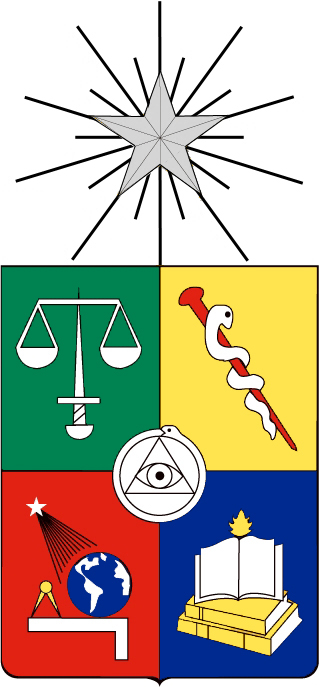
\includegraphics[width=2cm]{pics/escudocolor.png} % Replace "pics/escudocolor.png" with the filename and path of your logo image
        \vspace{1cm}
        
        {\Huge\textbf{Universidad de Chile}} \\
        \vspace{0.5cm}
        {\Large Departamento de Ciencias de la Computación} \\
        \vspace{2cm}
        
        {\Huge\textbf{Procesamiento de Lenguaje Natural}} \\
        \vspace{0.5cm}
        {\Large Apuntes de Clases} \\
        \vspace{2cm}
        
        {\Large Felipe Bravo-Márquez} \\
        \vspace{2cm}
        
        {\large \today}
    \end{center}
\end{titlepage}

\newpage

\thispagestyle{empty}

\newpage
\pagenumbering{roman}

\tableofcontents 
\newpage

\listoftables
\newpage
\listoffigures
\newpage


\thispagestyle{empty}


\pagenumbering{arabic}

%..................................................

\chapter*{Prefacio}
\addcontentsline{toc}{chapter}{Preface}
Este apunte es el resultado de cinco años de experiencia en la enseñanza del curso de Procesamiento de Lenguaje Natural en la Universidad de Chile\footnote{El repositorio del curso se encuentra en: \url{https://github.com/dccuchile/CC6205}}. El objetivo es proporcionar una introducción a esta disciplina, centrándose en las técnicas y conceptos fundamentales. Se ha realizado un esfuerzo por lograr un equilibrio entre las técnicas tradicionales, como los modelos de lenguaje de N-gramas, Naive Bayes y los modelos ocultos de Markov (HMM), y los enfoques modernos basados en redes neuronales profundas, como los vectores de palabras, las redes neuronales recurrentes (RNN), los transformers y los grandes modelos de lenguaje. Sin embargo, es importante mencionar que existen temas relevantes que no se incluyen en este material, como el etiquetado de datos, las gramáticas, las técnicas de parsing, así como discusiones sobre tareas más específicas como el question answering.

El contenido se ha recopilado de diversas fuentes. Los temas relacionados con las redes neuronales se basan principalmente en el libro "Neural Network Methods for Natural Language Processing" de Goldberg \cite{goldberg2017neural}. Los temas no relacionados con las redes neuronales, como los modelos probabilísticos del lenguaje, Naive Bayes y HMM, se han tomado del curso de Michael Collins de Columbia \cite{collins2013language} y del borrador de la tercera edición del libro de Dan Jurafsky y James H. Martin \cite{JurafskyBook}. Además, algunos capítulos se han adaptado de tutoriales en línea y otros cursos, como el curso de Stanford de Christopher Manning\footnote{\url{http://web.stanford.edu/class/cs224n/}}. Las imágenes utilizadas se han extraído intencionalmente directamente de sus fuentes correspondientes. Algún día se diseñarán imágenes propias.

\chapter{Introducción}
\label{cap:intro}


El volumen de datos textuales digitalizados que se genera cada día es enorme (por ejemplo, la web, redes sociales, registros médicos, libros digitalizados). Por lo tanto, también crece la necesidad de traducir, analizar y gestionar esta avalancha de palabras y texto.

El procesamiento del lenguaje natural (PLN) es el campo que se encarga de diseñar métodos y algoritmos que toman como entrada o producen como salida datos de \textbf{lenguaje natural} no estructurado \cite{goldberg2017neural}. El PLN se centra en el diseño y análisis de algoritmos computacionales y representaciones para procesar el lenguaje humano \cite{jacobbook}.





Una tarea común de PLN es el Reconocimiento de Entidades Nombradas (NER, por sus siglas en inglés). Por ejemplo:

\begin{figure}[h]
	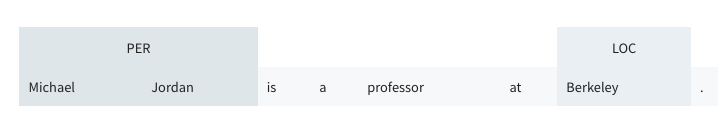
\includegraphics[scale=0.4]{pics/NER.png}
	\caption{Reconocimiento de Entidades Nombradas}
\end{figure}

El lenguaje humano es altamente ambiguo, como en las frases: "Comí pizza con amigos", "Comí pizza con aceitunas" o "Comí pizza con un tenedor". Además, el lenguaje está en constante cambio y evolución, como ocurre con los hashtags en Twitter.

\section{PLN y Lingüística Computacional}
PLN suele confundirse con otra disciplina hermana llamada Lingüística Computacional (LC). Si bien ambas están estrechamente relacionadas, tienen un foco distinto. La LC busca responder preguntas fundamentales sobre el lenguaje mediante el uso de la computación, es decir, cómo entendemos el lenguaje, cómo producimos lenguaje o cómo aprendemos lenguaje. Mientras que en PLN el foco está en resolver problemas específicos, tales como las transcripción automática del habla, la traducción automática, la extracción de información de documentos y el análisis de opiniones en redes sociales. Es importante señalar que en PLN, el éxito de una solución se mide en base métricas concretas (Ej: qué tan similar es la traducción automática a una hecha por un humano) independientemente si el modelo hace uso de alguna teoría lingüística.



El procesamiento del lenguaje natural (PLN) desarrolla métodos para resolver problemas prácticos relacionados con el lenguaje \cite{JohnsonMLSS}.

Algunos ejemplos son:

\begin{itemize}
  \item Reconocimiento automático del habla.
  \item Traducción automática.
  \item Extracción de información de documentos.
\end{itemize}

La lingüística computacional (LC) estudia los procesos computacionales subyacentes al lenguaje (humano).

\begin{itemize}
  \item ¿Cómo comprendemos el lenguaje?
  \item ¿Cómo producimos el lenguaje?
  \item ¿Cómo aprendemos el lenguaje?
\end{itemize}

El PLN y la LC utilizan métodos y modelos similares.


Aunque existe una superposición sustancial, hay una diferencia importante en el enfoque. La LC se centra en la lingüística respaldada por métodos computacionales (similar a la biología computacional o la astronomía computacional). En lingüística, el lenguaje es el objeto de estudio. El PLN se centra en resolver tareas bien definidas relacionadas con el lenguaje humano (como la traducción, la respuesta a consultas, las conversaciones). Si bien los conocimientos lingüísticos fundamentales pueden ser cruciales para realizar estas tareas, el éxito se mide en función de si y cómo se logra el objetivo (según una métrica de evaluación) \cite{jacobbook}.



El procesamiento del lenguaje natural y la lingüística computacional están estrechamente relacionados y se superponen en muchos aspectos. Ambos campos utilizan métodos y modelos similares para abordar problemas relacionados con el lenguaje humano. Sin embargo, la diferencia principal radica en el enfoque: la lingüística computacional se centra en la lingüística respaldada por métodos computacionales, mientras que el procesamiento del lenguaje natural se centra en resolver tareas prácticas relacionadas con el lenguaje. Ambos campos son fundamentales para comprender y aprovechar el poder del lenguaje humano en la era digital.


\section{Niveles de descripción lingüística}

El campo de la \textbf{descripción lingüística} abarca diferentes niveles:

\begin{itemize}
  \item \textbf{Fonética y fonología:} estudio de los sonidos del habla.
  \item \textbf{Morfología:} estudio de la estructura de las palabras.
  \item \textbf{Sintaxis:} estudio de la estructura de las oraciones.
  \item \textbf{Semántica:} estudio del significado de las palabras y oraciones.
  \item \textbf{Pragmática:} estudio del uso del lenguaje en el contexto.
\end{itemize}

El PLN puede abordar tareas en cada uno de estos niveles, pero a menudo se enfoca en niveles más altos de representación y comprensión.




\subsection{Fonética}

La fonética es la rama de la lingüística que se ocupa del estudio de los sonidos del lenguaje. Examina los órganos utilizados en la producción de sonidos, como la boca, la lengua, la garganta, la nariz, los labios y el paladar. Los sonidos del lenguaje se dividen en vocales y consonantes. Las vocales se producen con poca restricción del flujo de aire desde los pulmones, mientras que las consonantes implican alguna restricción o cierre en el tracto vocal \cite{JohnsonMLSS, fromkin2018introduction}. Además, el Alfabeto Fonético Internacional (AFI) proporciona una notación alfabética para representar los sonidos fonéticos.

\subsection{Fonología}

La fonología se centra en el estudio de cómo los sonidos del habla forman patrones y construyen significado. Los fonemas son las unidades básicas de sonido que diferencian el significado de las palabras. Por ejemplo, en inglés, la "p" y la "b" son fonemas distintos porque cambian el significado de las palabras en las que se encuentran. La fonología también examina las variaciones en la pronunciación de los sonidos en diferentes contextos y dialectos \cite{fromkin2018introduction}.

\subsection{Morfología}

La morfología se ocupa del estudio de la estructura interna de las palabras. Los morfemas son las unidades mínimas de significado que componen las palabras. Por ejemplo, en la palabra "deshacer", los morfemas son "des-", "hacer" y "-er". La morfología también se interesa por los procesos de formación de palabras, como la derivación, donde se agregan prefijos o sufijos a una palabra existente para formar una nueva palabra con un significado diferente \cite{JohnsonMLSS}.

\begin{itemize}
\item La morfología estudia la estructura de las palabras (por ejemplo, re+estructur+ando, in+olvid+able) \cite{JohnsonMLSS}
\item Morfema: el término lingüístico para la unidad más elemental de forma gramatical \cite{fromkin2018introduction}. Por ejemplo, morfología = morf + ología (la ciencia de).
\item Morfología derivativa: proceso de formar una nueva palabra a partir de una palabra existente, a menudo mediante la adición de un prefijo o sufijo.
\item La morfología derivativa exhibe una estructura jerárquica. Ejemplo: re+vital+iz+ación
\begin{figure}[h]
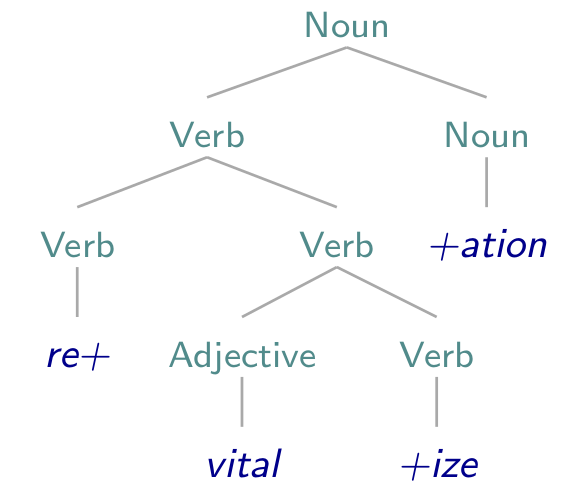
\includegraphics[scale = 0.2]{pics/morphology.png}
\end{figure}
\item El sufijo generalmente determina la categoría sintáctica (part-of-speech) de la palabra derivada.
\end{itemize}

\subsection{Sintaxis}

La sintaxis es el estudio de cómo las palabras se combinan para formar frases y oraciones gramaticales. Examina las reglas y estructuras que determinan la organización de las palabras en una oración y cómo influyen en el significado. La sintaxis también se ocupa de la relación entre las palabras y las funciones que desempeñan dentro de una oración. Por ejemplo, en la oración "El perro persigue al gato", "el perro" es el sujeto, "persigue" es el verbo y "al gato" es el complemento directo \cite{JohnsonMLSS}.

\begin{itemize}
\item La sintaxis estudia las formas en que las palabras se combinan para formar frases y oraciones \cite{JohnsonMLSS}
\begin{figure}[h]
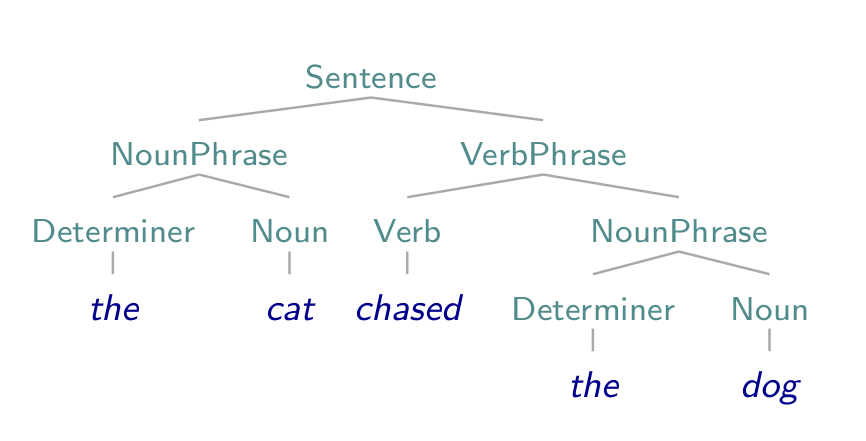
\includegraphics[scale = 0.3]{pics/parseTree1.png}
\end{figure}
\item El análisis sintáctico ayuda a identificar \textbf{quién hizo qué a quién}, un paso clave para comprender una oración.
\end{itemize}


\subsection{Semántica}

La semántica es el estudio del significado de las palabras, frases y oraciones, examinando cómo se construye e interpreta este significado en el contexto del lenguaje. Además, la semántica se interesa por los roles semánticos, que indican la función de cada entidad en una oración. Por ejemplo, en la oración "El niño cortó la cuerda con una navaja", "el niño" es el agente, "la cuerda" es el tema y "una navaja" es el instrumento \cite{JohnsonMLSS}.

La semántica se enfoca en el significado de las palabras, frases y oraciones. Estudia cómo se construye e interpreta este significado en el contexto del lenguaje. Además, dentro de la semántica, se analizan los roles semánticos, los cuales indican la función que desempeña cada entidad en una oración. Por ejemplo, en la oración "El niño cortó la cuerda con una navaja", se identifican distintos roles semánticos: "el niño" como el agente, "la cuerda" como el tema y "una navaja" como el instrumento utilizado \cite{JohnsonMLSS}.


En resumen:
\begin{itemize}
\item La semántica estudia el significado de las palabras, frases y oraciones \cite{JohnsonMLSS}.
\item Dentro de la semántica, se analizan los roles semánticos, que indican el papel desempeñado por cada entidad en una oración.
\item Algunos ejemplos de roles semánticos son: \textcolor[rgb]{0.00,0.00,1.00}{\textbf{agente}} (la entidad que realiza la acción), \textcolor[rgb]{1.00,0.00,0.00}{\textbf{tema}} (la entidad involucrada en la acción) y \textcolor[rgb]{0.00,1.00,0.00}{\textbf{instrumento}} (otra entidad utilizada por el agente para llevar a cabo la acción).
\item En la oración "El niño cortó la cuerda con una navaja", se puede identificar el agente como \textcolor[rgb]{0.00,0.00,1.00}{\textbf{el niño}}, el tema como \textcolor[rgb]{1.00,0.00,0.00}{\textbf{la cuerda}} y el instrumento como \textcolor[rgb]{0.00,1.00,0.00}{\textbf{una navaja}}.
\item Además de los roles semánticos, la semántica también abarca las relaciones léxicas, que son las relaciones entre diferentes palabras \cite{yule2016study}.
\item Algunos ejemplos de relaciones léxicas incluyen la sinonimia (conceal/hide), la antonimia (shallow/deep) y la hiponimia (perro/animal).
\end{itemize}


\subsection{Pragmática}

La pragmática se centra en cómo el contexto influye en la interpretación y el significado de las expresiones lingüísticas. Examina cómo se utilizan las expresiones lingüísticas en situaciones reales y cómo los hablantes interpretan el significado implícito. Por ejemplo, la oración "Hace frío aquí" puede interpretarse como una sugerencia implícita de cerrar las ventanas \cite{fromkin2018introduction}.


\section{Procesamiento del Lenguaje Natural y Aprendizaje Automático}

Comprender y producir el lenguaje computacionalmente es extremadamente complejo.  La tecnología más exitosa actualmente para abordar PLN es el aprendizaje automático supervisado que consiste en una familia de algoritmos que “aprenden” a construir la respuesta del problema en cuestión en base a encontrar patrones en datos de entrenamiento etiquetados. Por ejemplo, si queremos tener un modelo que nos diga si un tweet tiene un sentimiento positivo o negativo respecto a un producto, primero necesito  etiquetar manualmente un conjunto de tweets con su sentimiento asociado. Luego debo entrenar un algoritmo de aprendizaje sobre estos datos para poder predecir de manera automática el sentimiento asociado a tweets desconocidos. Como se podrán imaginar, el etiquetado de datos es una parte fundamental de la solución y puede ser un proceso muy costoso, especialmente cuando se requiere conocimiento especializado para definir la etiqueta.

Aunque los seres humanos somos grandes usuarios del lenguaje, también somos muy malos para comprender y describir formalmente las reglas que rigen el lenguaje.

Entender y producir lenguaje utilizando computadoras es altamente desafiante. Los métodos más conocidos para lidiar con datos de lenguaje se basan en el aprendizaje automático supervisado.

El aprendizaje automático supervisado consiste en intentar inferir patrones y regularidades a partir de un conjunto de pares de entrada y salida preanotados (también conocido como conjunto de datos de entrenamiento).

\paragraph{Conjunto de Datos de Entrenamiento: Datos de NER CoNLL-2003}

Cada línea contiene un token, una etiqueta de parte de la oración, una etiqueta de sintagma y una etiqueta de entidad nombrada.
\begin{center}
\begin{verbatim}
U.N.         NNP  I-NP  I-ORG
official     NN   I-NP  O
Ekeus        NNP  I-NP  I-PER
heads        VBZ  I-VP  O
for          IN   I-PP  O
Baghdad      NNP  I-NP  I-LOC
.            .    O     O
\end{verbatim}
\end{center}

\footnotemark{Fuente: \url{https://www.clips.uantwerpen.be/conll2003/ner/}}

\section{Desafíos del Lenguaje}

Existen tres propiedades desafiantes del lenguaje: la discreción, la composicionalidad y la dispersión.

\textbf{Discreción}: no podemos inferir la relación entre dos palabras a partir de las letras que las componen (por ejemplo, hamburguesa y pizza).

\textbf{Composicionalidad}: el significado de una oración va más allá del significado individual de sus palabras.

\textbf{Dispersión}: la forma en que las palabras (símbolos discretos) pueden combinarse para formar significados es prácticamente infinita.



\section{Ejemplo de tareas NLP}


\paragraph{Clasificación de temas}

La clasificación de temas es una tarea de Procesamiento del Lenguaje Natural (PLN) en la cual se asigna a un documento una de varias categorías, como deportes, política, cotilleos o economía. Las palabras presentes en los documentos brindan pistas importantes sobre su tema. Sin embargo, redactar reglas para esta tarea es un desafío debido a la complejidad del lenguaje. La anotación de datos, en la cual los lectores clasifican los documentos por temas, puede ayudar a generar conjuntos de datos de entrenamiento para algoritmos de aprendizaje automático supervisado. Estos algoritmos aprenden patrones de uso de palabras que facilitan la categorización de los documentos.

\begin{itemize}
\item Clasificar un documento en una de las cuatro categorías: Deportes, Política, Cotilleos y Economía.
\item Las palabras en los documentos proporcionan indicios muy sólidos.
\item ¿Qué palabras brindan qué indicios?
\item Elaborar reglas para esta tarea resulta bastante desafiante.
\item No obstante, los lectores pueden categorizar fácilmente varios documentos según su tema (anotación de datos).
\item Un algoritmo de aprendizaje automático supervisado puede identificar los patrones de uso de palabras que ayudan a categorizar los documentos.
\end{itemize}
\paragraph{Análisis de Sentimiento}

El análisis de sentimientos se refiere a la aplicación de técnicas de Procesamiento del Lenguaje Natural (PLN) para identificar y extraer información subjetiva de conjuntos de datos textuales. Un desafío común en el análisis de sentimientos es la clasificación de la polaridad a nivel de mensaje (MPC), donde las frases se clasifican automáticamente en categorías positivas, negativas o neutrales. Las soluciones más avanzadas utilizan modelos de aprendizaje automático supervisado entrenados con ejemplos anotados manualmente.

En este tipo de clasificación, es habitual emplear el aprendizaje supervisado, siendo las Máquinas de Vectores de Soporte (SVM) una opción popular. El objetivo de las SVM es encontrar un hiperplano que separe las clases con el margen máximo, logrando la mejor separación entre las clases positivas, negativas y neutrales \cite{jacobbook}.

\begin{itemize}
  \item Aplicación de técnicas de \textbf{PLN} para identificar y extraer información subjetiva de conjuntos de datos textuales.
  \item Clasificación automática de frases en las categorías \textcolor[rgb]{0.00,0.00,1.00}{\textbf{positiva}}, \textcolor[rgb]{1.00,0.00,0.00}{\textbf{negativa}} o \textcolor[rgb]{0.00,1.00,0.00}{\textbf{neutral}}.

     \begin{figure}[h]
        	
\includegraphics[scale = 0.15]{pics/sent.png}
        \end{figure}

  \item Las soluciones más avanzadas emplean modelos de aprendizaje automático \textbf{supervisado}, entrenados con ejemplos \textbf{anotados manualmente} \cite{Mohammad2013}.
\end{itemize}


\begin{figure}[h]
        	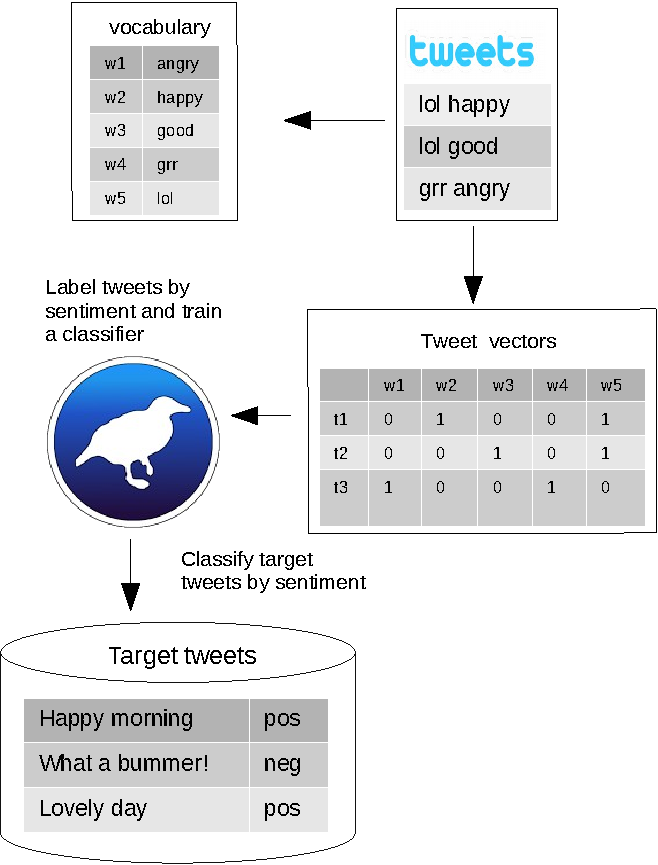
\includegraphics[scale = 0.5]{pics/bagOfwordsClassification.pdf}
        \end{figure}


\begin{itemize}


\item Idea: Encontrar un hiperplano que separe las clases con el margen máximo (mayor separación).

     \begin{figure}[h]
        	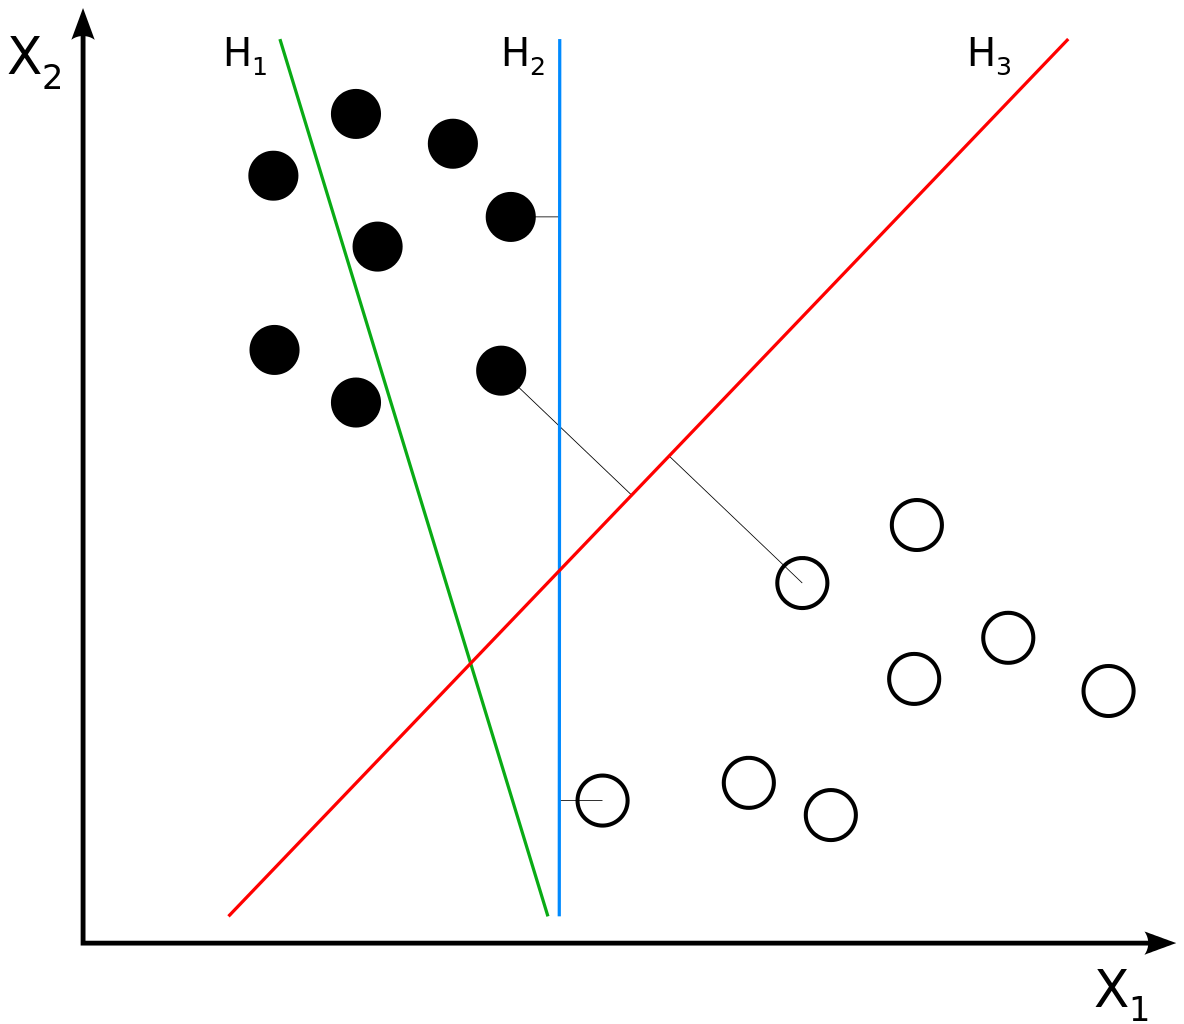
\includegraphics[scale = 0.15]{pics/SVM.png}
        \end{figure}

\item $H_3$ separa las clases con el margen máximo.

\end{itemize}


\subsection{Lingüística y Procesamiento del Lenguaje Natural (PNL)}

El conocimiento de las estructuras lingüísticas es fundamental para el diseño de características y el análisis de errores en el Procesamiento del Lenguaje Natural (PNL). Los enfoques de aprendizaje automático en PNL se basan en características que describen y generalizan las instancias de uso del lenguaje. El conocimiento lingüístico orienta la selección y el diseño de estas características, ayudando al algoritmo de aprendizaje automático a encontrar correlaciones entre el uso del lenguaje y las etiquetas objetivo \cite{bender2013linguistic}.

\begin{itemize}
  \item El conocimiento de las estructuras lingüísticas es importante para el diseño de características y el análisis de errores en PNL \cite{bender2013linguistic}.
  \item Los enfoques de aprendizaje automático en PNL requieren características que puedan describir y generalizar el uso del lenguaje.
  \item El objetivo es guiar al algoritmo de aprendizaje automático para encontrar correlaciones entre el uso del lenguaje y el conjunto de etiquetas objetivo.
  \item El conocimiento sobre las estructuras lingüísticas puede influir en el diseño de características para los enfoques de aprendizaje automático en PNL.
\end{itemize}

El PNL plantea diversos desafíos, como los costos de anotación, las variaciones de dominio y la necesidad de actualizaciones continuas. La anotación manual requiere mucho trabajo y tiempo. Las variaciones de dominio implican aprender patrones diferentes para diferentes corpus de texto. Los modelos entrenados en un dominio pueden no funcionar bien en otro. Además, los modelos de PNL pueden volverse obsoletos a medida que el uso del lenguaje evoluciona con el tiempo.




\section{Desafíos en el Procesamiento del Lenguaje Natural (PNL)}

\begin{itemize}
   \item \textbf{Costos de Anotación}: la anotación manual es \textbf{laboriosa} y \textbf{consume mucho tiempo}.
   \item \textbf{Variaciones de Dominio}: el patrón que queremos aprender puede variar de un corpus a otro (por ejemplo, deportes, política).

   \item ¡Un modelo entrenado con datos anotados de un dominio no necesariamente funcionará en otro!
   \item Los modelos entrenados pueden quedar desactualizados con el tiempo (por ejemplo, nuevos hashtags).
\end{itemize}

\paragraph{Variación de Dominio en el Análisis de Sentimiento}
\begin{enumerate}
   \item Para mí, la cola era bastante \textcolor[rgb]{0.00,0.00,1.00}{\textbf{pequeña}} y solo tuve que esperar unos 20 minutos, ¡pero valió la pena! :D @raynwise
   \item Extraña espacialidad en Stuttgart. La habitación del hotel es tan \textcolor[rgb]{1.00,0.00,0.00}{\textbf{pequeña}} que apenas puedo moverme, pero los alrededores son inhumanamente vastos y largos bajo construcción.
\end{enumerate}

\paragraph{Superando los costos de anotación de datos}
Supervisión Distant:
\begin{itemize}
   \item Etiquetar automáticamente datos no etiquetados (\textbf{API de Twitter}) utilizando un método heurístico.
   \item \textbf{Enfoque de Anotación de Emoticonos (EAA)}: los tweets con emoticonos positivos \textcolor[rgb]{0.00,0.00,1.00}{\textbf{:)}} o negativos \textcolor[rgb]{1.00,0.00,0.00}{\textbf{:(}} se etiquetan según la polaridad indicada por el emoticono~\cite{Read2005}.
   \item El emoticono se \textbf{elimina} del contenido.
   \item Este enfoque también se ha ampliado utilizando hashtags como \#anger y emojis.
   \item No es trivial encontrar técnicas de supervisión distante para todo tipo de problemas de PNL.
\end{itemize}

\paragraph{Crowdsourcing}
\begin{itemize}
   \item Confiar en servicios como \textbf{Amazon Mechanical Turk} o \textbf{Crowdflower} para solicitar a la \textbf{multitud} que anote datos.
   \item Esto puede resultar costoso.
   \item Es difícil garantizar la calidad de las anotaciones.
\end{itemize}

\section{Estudio de caso: Clasificación de sentimientos en tweets}

\begin{itemize}
   \item En 2013, el taller de Evaluación Semántica (SemEval) organizó la tarea de "Análisis de sentimientos en Twitter" \cite{Semeval2013}.
   \item La tarea se dividió en dos sub-tareas: el nivel de expresión y el nivel del mensaje.
   \item Nivel de expresión: se centró en determinar la polaridad del sentimiento de un mensaje según una entidad marcada dentro de su contenido.
   \item Nivel del mensaje: se debía determinar la polaridad según el mensaje en general.
   \item Los organizadores lanzaron conjuntos de datos de entrenamiento y prueba para ambas tareas \cite{Semeval2013}.
\end{itemize}

\paragraph{El sistema NRC}
\begin{itemize}
   \item El equipo que logró el mejor rendimiento en ambas tareas, entre 44 equipos, fue el equipo \emph{NRC-Canada} \cite{Mohammad2013}.
   \item El equipo propuso un enfoque supervisado utilizando un clasificador SVM lineal con las siguientes características hechas a mano para representar los tweets:
   \begin{enumerate}
      \item N-gramas de palabras.
      \item N-gramas de caracteres.
      \item Etiquetas de partes del discurso.
      \item Agrupaciones de palabras entrenadas con el método de agrupamiento de Brown \cite{brown1992class}.
      \item El número de palabras alargadas (palabras con un carácter repetido más de dos veces).
      \item El número de palabras con todas las letras en mayúscula.
      \item La presencia de emoticonos positivos o negativos.
      \item El número de negaciones individuales.
      \item El número de secuencias contiguas de puntos, signos de interrogación y signos de exclamación.
      \item Características derivadas de lexicones de polaridad \cite{Mohammad2013}. Dos de estos lexicones se generaron utilizando el método PMI a partir de tweets anotados con hashtags y emoticonos.
   \end{enumerate}
\end{itemize}

\section{Ingeniería de características y Aprendizaje Profundo}

\begin{itemize}
   \item Hasta 2014, la mayoría de los sistemas de PNL de última generación se basaban en ingeniería de características + modelos de aprendizaje automático superficiales (por ejemplo, SVM, HMM).
   \item Diseñar las características de un sistema de PNL ganador requiere mucho conocimiento específico del dominio.
   \item El sistema NRC se construyó antes de que el aprendizaje profundo se hiciera popular en PNL.
   \item Por otro lado, los sistemas de Aprendizaje Profundo se basan en redes neuronales para aprender automáticamente buenas representaciones.
\end{itemize}

\paragraph{Ingeniería de características y Aprendizaje Profundo}

\begin{figure}[h]
   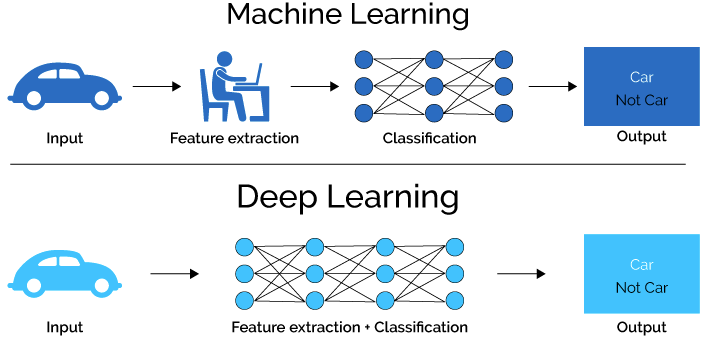
\includegraphics[scale = 0.25]{pics/MLvsDL.png}
\end{figure}

\begin{itemize}
   \item El Aprendizaje Profundo proporciona resultados de última generación en la mayoría de las tareas de PNL.
   \item Grandes cantidades de datos de entrenamiento y máquinas GPU

 multicore más rápidas son clave en el éxito del aprendizaje profundo.
   \item Las \textbf{redes neuronales} y las \textbf{incrustaciones de palabras} desempeñan un papel fundamental en los modelos modernos de PNL.

\end{itemize}

\paragraph{Aprendizaje Profundo y Conceptos Lingüísticos}
\begin{itemize}
   \item Si los modelos de aprendizaje profundo pueden aprender representaciones automáticamente, ¿siguen siendo útiles los conceptos lingüísticos (por ejemplo, sintaxis, morfología)?
   \item Algunos defensores del aprendizaje profundo argumentan que estas propiedades lingüísticas inferidas y diseñadas manualmente no son necesarias, y que la red neuronal aprenderá estas representaciones intermedias (o equivalentes o mejores) por sí misma \cite{goldberg2016primer}.
   \item Aún no hay un consenso definitivo al respecto.
   \item Goldberg cree que muchos de estos conceptos lingüísticos pueden ser inferidos por la red por sí misma si se le proporciona suficiente cantidad de datos.
   \item Sin embargo, en muchos otros casos no disponemos de suficientes datos de entrenamiento para la tarea que nos interesa, y en estos casos proporcionar a la red los conceptos generales más explícitos puede ser muy valioso.
\end{itemize}

\section{Historia}

Los orígenes de PLN se remontan a los años 50 con el famoso test de Alan Turing: una máquina será considerada inteligente cuando sea capaz de conversar con una persona sin que esta pueda determinar si está hablando con una máquina o un ser humano. A lo largo de su historia la disciplina ha tenido tres grandes períodos: 1) el racionalismo, 2) el empirismo, y 3) el aprendizaje profundo [Deng y Liu, 2018] que describimos a continuación.

El racionalismo abarca desde 1950 a 1990, donde las soluciones consistían en diseñar reglas manuales para incorporar mecanismos de conocimiento y razonamiento. Un ejemplo emblemático es el agente de conversación (o chatbot) ELIZA desarrollado por Joseph Weizenbaum que simulaba  un psicoterapeuta rogeriano. Luego, a partir de la década de los 90s, el diseño de métodos estadísticos y de aprendizaje automático construidos sobre corpus llevan a PLN hacia un enfoque empirista. Las reglas ya no se construyen sino que se “aprenden” a partir de datos etiquetados.  Algunos modelos representativos de esta época son los filtros de spam basados en modelos lineales, las cadenas de Markov ocultas para la extracción de categorías sintácticas y los modelos probabilísticos de IBM para la traducción automática. Estos modelos se caracterizaban por ser poco profundos en su estructura de parámetros y por depender de características manualmente diseñadas para representar la entrada.

A partir del año 2010, las redes neuronales artificiales, que son una familia de modelos de aprendizaje automático, comienzan a mostrar resultados muy superiores en varias tareas emblemáticas de PLN [Collobert et al., 2011]. La idea de estos modelos es representar la entrada (el texto) con una jerarquía de parámetros (o capas) que permiten encontrar representaciones idóneas para la tarea en cuestión, proceso al cual se refiere como “aprendizaje profundo”. Estos modelos se caracterizan por tener muchos más parámetros que los modelos anteriores (superando la barrera del millón en algunos casos) y requerir grandes volúmenes de datos para su entrenamiento. Una gracia de estos modelos es que pueden ser pre-entrenados con texto no etiquetado como libros, Wikipedia, texto de redes sociales y de la Web para encontrar representaciones iniciales de palabras y oraciones (a lo que conocemos como word embeddings),  las cuales pueden ser posteriormente adaptadas para la tarea objetivo donde sí se tienen datos etiquetados (Proceso conocido como transfer learning). Aquí destacamos modelos como Word2Vec [Mikolov 2013], BERT  [Devlin 2018] y GPT-3  [Brown 2020].

Este tipo de modelos ha ido perfeccionándose en los últimos años, llegando a obtener resultados cada vez mejores para casi todos los problemas del área [NLPProgress]. Sin embargo, este progreso no ha sido libre de controversias. El  aumento exponencial en la cantidad de parámetros de cada nuevo modelo respecto a su predecesor, hace que los recursos computacionales y energéticos necesarios para construirlos sólo estén al alcance de unos pocos. Además, varios estudios han mostrado que estos modelos aprenden y reproducen los sesgos y prejuicios (ej: género, religión, racial) presentes en los textos a partir de los cuales se entrenan. Sin ir más lejos, la investigadora  Timmnit Gebru fue despedida de Google  cuando se le negó el permiso para publicar un artículo que ponía de manifiesto estos problemas [Bender 2021].


El progreso de la PNL se puede dividir en tres oleadas principales: 1) racionalismo, 2) empirismo y 3) aprendizaje profundo \cite{deng2018deep}.
\begin{itemize}
   \item [1950 - 1990] Racionalismo: se enfocaba en diseñar reglas hechas a mano para incorporar conocimiento y mecanismos de razonamiento en sistemas de PNL inteligentes (por ejemplo, ELIZA para simular a un psicoterapeuta Rogeriano, MARGIE para estructurar información del mundo real en ontologías de conceptos).
   \item [1991 - 2009] Empirismo: se caracteriza por la explotación de corpora de datos y modelos de aprendizaje automático y estadísticos (superficiales) (por ejemplo, Naive Bayes, HMMs, modelos de traducción IBM).
   \item [2010 - ] Aprendizaje Profundo: la ingeniería de características (considerada como un cuello de botella) se reemplaza con el aprendizaje de representaciones y/o redes neuronales profundas (por ejemplo, \url{https://www.deepl.com/translator}). Un artículo muy influyente en esta revolución: \cite{collobert2011natural}.
\end{itemize}

\footnotetext{Las fechas son aproximadas.}

\section{Conclusiones}


En este capítulo, hemos explorado el desafío de entender y producir lenguaje utilizando computadoras. El aprendizaje automático supervisado es una de las principales técnicas utilizadas para abordar este desafío. Además, hemos discutido las propiedades desafiantes del lenguaje, como la discreción, la composicionalidad y la dispersión. Estos aspectos nos muestran la complejidad inherente al procesamiento del lenguaje natural y nos desafían a encontrar soluciones efectivas.




\chapter{Modelo de Espacio Vectorial y Recuperación de Información}
\label{cap_ir}

En este capítulo, exploraremos las primeras técnicas utilizadas para representar el lenguaje en forma vectorial. Para contextualizar esto, planteamos las siguientes preguntas:

\begin{itemize}
   \item ¿Cómo recuperan los motores de búsqueda, como Duckduckgo o Google, los documentos relevantes a partir de una consulta dada?
   \item ¿Cómo pueden las empresas procesar las reclamaciones dejadas por sus usuarios en sus portales web?
\end{itemize}

Estas preguntas suelen abordarse desde dos disciplinas relacionadas:

\begin{itemize}
   \item \emph{Recuperación de Información}: ciencia que se ocupa de buscar información en colecciones de documentos.
   \item \emph{Minería de Texto}: extracción automática de conocimiento a partir de texto.
\end{itemize}

Ambas disciplinas están estrechamente vinculadas al PLN, y las fronteras entre estos campos no siempre están claras.

\section{Tokens y Tipos}

El primer paso en el procesamiento de texto es, generalmente, la \textbf{tokenización}, que consiste en dividir una oración o documento en fragmentos llamados \emph{tokens}. A menudo, se acompañan otras transformaciones adicionales, como la eliminación de caracteres especiales (por ejemplo, puntuación), la conversión de todo el texto a minúsculas y otras operaciones descritas en este capítulo.

\paragraph{Ejemplo}

Entrada: ``Me gustan los lenguajes humanos y los lenguajes de programación.''

Tokens: [Me] [gustan] [los] [lenguajes] [humanos] [y] [los] [lenguajes] [de] [programación]

\subsection{Tipos}

Un \emph{tipo} es una clase de \emph{token} que contiene una secuencia única de caracteres. Los tipos se obtienen identificando los tokens únicos dentro del documento.

Por ejemplo, para la oración anterior, los tipos serían: [Me] [gustan] [los] [lenguajes] [humanos] [y] [de] [programación]. Observemos que el token \emph{lenguajes} se incluye solo una vez en la lista de tipos.

\paragraph{Extracción de Vocabulario}

Un \emph{término} es un \emph{tipo} normalizado. La normalización implica la creación de clases de equivalencia para diferentes \emph{tipos}, por ejemplo, cuando tratamos de manera indistinta dos tokens que difieren solo en el uso de mayúsculas (hombre y Hombre). El vocabulario $V$ es el conjunto de términos (tokens únicos normalizados) dentro de una colección de documentos o corpus $D$.

\section{Eliminación de Stopwords}

Con el fin de reducir el tamaño del vocabulario y eliminar términos que no aportan mucha información, se eliminan los términos que ocurren con alta frecuencia en el corpus (o colección de documentos). Estos términos se llaman \emph{stopwords} e incluyen artículos, pronombres, preposiciones y conjunciones.

Ejemplo de stopwords: [un, una, y, cualquier, no, el, en].

Es importante tener en cuenta que la eliminación de stopwords puede ser inconveniente en muchas tareas de procesamiento del lenguaje natural. Por ejemplo, en la oración ``No me gusta la pizza'', al eliminar la negación, se pierde información valiosa sobre el sentimiento de la oración.

\section{Stemming}

Es un proceso de normalización de términos en el cual los términos se transforman a su raíz con el objetivo de reducir el tamaño del vocabulario. Se lleva a cabo aplicando reglas de reducción de palabras. La Tabla~\ref{tab:porter} muestra  algunas reglas del algortimo de Porter para el inglés con ejemplos de aplicación:

\begin{table}[h]
\centering
\begin{tabular}{|l|l|}
\hline
Regla & Ejemplo \\
\hline
SSES $\rightarrow$ SS & caresses $\rightarrow$ caress \\
IES $\rightarrow$ I & ponies $\rightarrow$ poni \\
SS $\rightarrow$ SS & caress $\rightarrow$ caress \\
S $\rightarrow$ & cats $\rightarrow$ cat \\
\hline
\end{tabular}
\caption{Ejemplos del Algortimo de Porter}
\label{tab:porter}
\end{table}

A continuación se muestra ejemplo usando el método de stemming Snowball para español para el lenguaje \textbf{python} usando la biblioteca \textbf{nltk}.

\begin{verbatim}
from nltk import word_tokenize
from nltk.stem import SnowballStemmer
stemmer = SnowballStemmer('spanish')
texto = 'Me gustan los lenguajes humanos y los lenguajes de programación'
def stem_sentence(text):
    return ' '.join([stemmer.stem(i) for i in word_tokenize(text)])    
print(stem_sentence(texto))
>>
me gust los lenguaj human y los lenguaj de program
\end{verbatim}



\section{Lematización}
Otra estrategia de normalización de términos. También transforma las palabras en sus raíces.  Realiza un análisis morfológico utilizando diccionarios de referencia (tablas de búsqueda) para crear clases de equivalencia entre \emph{tipos}. Por ejemplo, para el token \emph{yendo}, una regla de stemming devolvería el término \emph{yend}, mientras que a través de la lematización obtendríamos el término \emph{ir}.

Veamos a continuación el resultado de aplicar lematización a la misma oración anterior con la biblioteca \textbf{spacy}:

\begin{verbatim}
# python -m spacy download es_core_news_sm
import spacy
nlp = spacy.load('es_core_news_sm')

def lemmatizer(text):  
  doc = nlp(text)
  return ' '.join([word.lemma_ for word in doc])

print(lemmatizer(texto))
>>
yo gustar el lenguaje humano y el lenguaje de programación
\end{verbatim}



\section{Ley de Zipf}
La Ley de Zipf, propuesta por George Kingsley Zipf en \cite{zipf1935}, es una ley empírica que describe la frecuencia de los términos en una colección de documentos (corpus). Según esta ley, la frecuencia $f$ de un término en un corpus es inversamente proporcional a su posición $r$ en una tabla de frecuencias ordenada:

\begin{equation}
f = \frac{cf}{r^{\beta}}
\end{equation}

Aquí, $cf$ es una constante dependiente de la colección y $\beta > 0$ es un factor de decaimiento. Cuando $\beta = 1$, la frecuencia sigue exactamente la Ley de Zipf, de lo contrario, sigue una distribución similar a la de Zipf. Esta ley nos indica que algunas palabras se utilizan con mucha más frecuencia que otras en un corpus. La Ley de Zipf se clasifica como una distribución de ley de potencia, que es un tipo de distribución de cola larga.

\begin{figure}[h!]
\centering
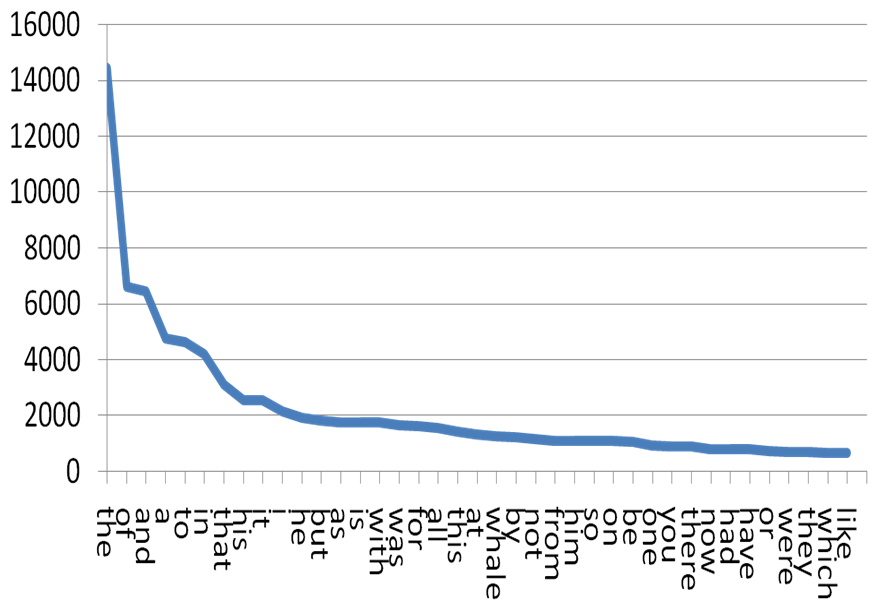
\includegraphics[scale=0.5]{pics/zipf1.png}
\caption{Ley de Zipf.}
\end{figure}

Cuando trazamos un gráfico en escala logarítmica ($log$-$log$), se obtiene una línea recta con una pendiente de $-\beta$. Esta relación logarítmica es útil para identificar las palabras más frecuentes en un corpus y construir una lista de stopwords.


\section{Listas de posteo y el índice invertido}
Sea $D$ una colección de documentos y $V$ el vocabulario de todos los términos extraídos de la colección:

\begin{itemize}
\item La lista de posteo de un término es la lista de todos los documentos donde el término aparece al menos una vez. Los documentos se identifican por sus identificadores.
\item Un índice invertido es una estructura de datos tipo diccionario que mapea los términos $t_{i} \in V$ con sus listas de posteo correspondientes.
\begin{displaymath}
<\text{término}> \rightarrow <\text{idDocumento}>^*
\end{displaymath}
\end{itemize}

\begin{figure}[h!]
\centering
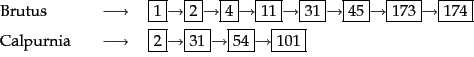
\includegraphics[scale=0.6]{pics/invFile.png}
\caption{Índice invertido}
\end{figure}

\section{Motores de búsqueda web}

Un motor de búsqueda es un sistema de recuperación de información diseñado para buscar información en la web (satisfacer necesidades de información) \cite{manning2008}. Sus componentes básicos son:

\begin{itemize}
\item Crawler: un robot que navega por la web según una estrategia definida. Por lo general, comienza navegando por un conjunto de sitios web iniciales (semillas) y continúa navegando a través de sus enlaces.
\item Indexador: se encarga de mantener un índice invertido con el contenido de las páginas recorridas por el rastreador.
\item Procesador de consultas: se encarga de procesar las consultas de los usuarios y buscar en el índice los documentos más relevantes para una consulta.
\item Función de ranking: la función utilizada por el procesador de consultas para ordenar los documentos indexados en la colección por relevancia según una consulta.
\item Interfaz de usuario: recibe la consulta como entrada y devuelve los documentos ordenados por relevancia.
\end{itemize}

\begin{figure}[h!]
\centering
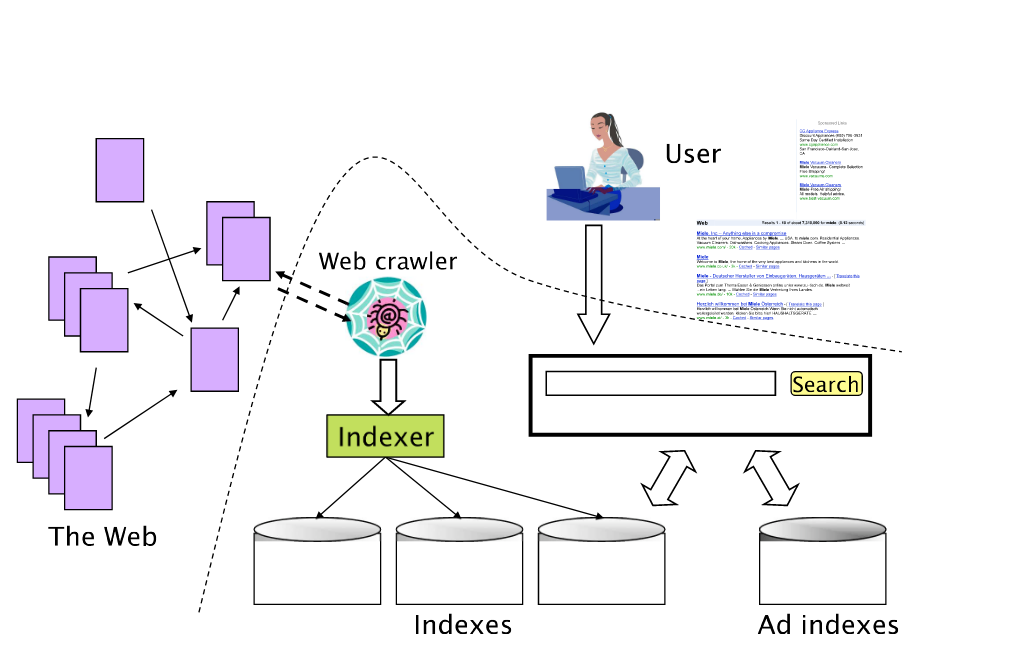
\includegraphics[scale=0.25]{pics/searchengine.png}
\caption{Los diversos componentes de un motor de búsqueda web \cite{manning2008}.}
\end{figure}


\section{El modelo de espacio vectorial}
Para clasificar consultas o medir la similitud entre dos documentos, necesitamos una métrica de similitud. Los documentos pueden ser \textit{representados} como vectores de términos, donde cada término es una dimensión del vector \cite{salton1975vector}. Documentos con diferentes palabras y longitudes residirán en el mismo espacio vectorial. Este tipo de representaciones se llaman \emph{Bolsa-de-palabras} (Bag of Words). En las representaciones de bolsa de palabras, se pierde el orden de las palabras y la estructura lingüística de una oración.

El valor de cada dimensión es un peso que representa la relevancia del término $t_{i}$ en el documento $d$.
\begin{equation}
d_{j} \rightarrow \overrightarrow{d_{j}}=(w(t_{1},d_{j}),...,w(t_{|V|},d_{j}))
\end{equation}

¿Cómo podemos modelar la información que aporta un término a un documento? Necesitamos formas de ponderar eso.

\subsection{Frecuencia de Término - Frecuencia Inversa de Documento}
Sea $tf_{i,j}$ la frecuencia del término $t_{i}$ en el documento $d_{j}$.  Un término que ocurre 10 veces debería proporcionar más información que uno que ocurre solo una vez. ¿Qué ocurre cuando tenemos documentos que son mucho más largos que otros? Podemos normalizar dividiendo por la frecuencia máxima del término en el documento.
\begin{displaymath}
ntf_{i,j}=\frac{tf_{i,j}}{\max_i (tf_{i,j})}
\end{displaymath}

Ahora podemos preguntarnos ¿un término que ocurre en muy pocos documentos proporciona más o menos información que uno que ocurre varias veces? Por ejemplo, el documento \emph{El respetado alcalde de Pelotillehue}. El término \emph{Pelotillehue} ocurre en menos documentos que el término \emph{alcalde}, por lo que debería ser más descriptivo.

Sea $N$ el número de documentos en la colección y $n_{i}$ el número de documentos que contienen el término $t_{i}$, definimos la frecuencia inversa de documento ($idf$) de $t_{i}$ de la siguiente manera:
\begin{displaymath}
idf_{t_{i}}= \log_{10}\left(\frac{N}{n_{i}}\right)
\end{displaymath}

Un término que aparece en todos los documentos tendría $idf=0$, y uno que aparece en el $10\%$ de los documentos tendría $idf=1$. El modelo $tf$-$idf$ combina los valores de $tf$ e $idf$, y resulta en los siguientes pesos $w$ para un término en un documento:
\begin{displaymath}
w(t_{i},d_{j})=tf_{i}\times \log_{10}\left(\frac{N}{n_{i}}\right)
\end{displaymath}

Las consultas de los motores de búsqueda también pueden ser modeladas como vectores. Sin embargo, en promedio, las consultas suelen tener entre 2 y 3 términos. Para evitar tener demasiadas dimensiones nulas, los vectores de consulta pueden suavizarse de la siguiente manera:
\begin{displaymath}
w(t_{i},d_{j})=(0.5+0.5\times tf_{i,j})\log_{10}\left(\frac{N}{n_{i}}\right)
\end{displaymath}

\subsection{Similitud entre vectores}
Representar consultas y documentos como vectores permite calcular su similitud. Un enfoque podría ser utilizar la distancia euclidiana. El enfoque común es calcular el coseno del ángulo entre los dos vectores. Si ambos documentos son iguales, el ángulo sería $0$ y su coseno sería $1$. Por otro lado, si son ortogonales, el coseno es $0$. La similitud del coseno se calcula de la siguiente manera:
\begin{displaymath}
\text{similitud del coseno}(\vec{d}{1},\vec{d}{2})= \frac{\vec{d}{1}\cdot \vec{d}{2}}{|\vec{d}{1}|\times|\vec{d}{2}|} = \frac{\sum_{i=1}^{|V|}(w(t_{i},d_{1})\times w(t_{i},d_{2}))}{\sqrt{\sum_{i=1}^{|V|} w(t_{i},d_{1})^2}\times \sqrt{\sum_{i=1}^{|V|} w(t_{i},d_{2})^2}}
\end{displaymath}

Esto se llama incorrectamente ``distancia del coseno''. En realidad, es una métrica de similitud pues entre más cerca dos vectores mayor es el valor asociado. Nótese que la similitud del coseno normaliza los vectores por su norma euclidiana $||\vec{d}||_{2}$.

\begin{figure}[h!]
\centering
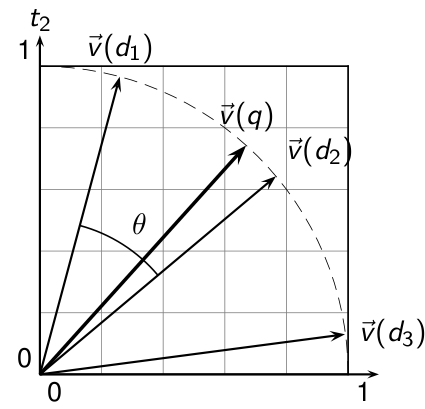
\includegraphics[scale=0.5]{pics/cos.png}
\caption{Similitud del coseno.}
\end{figure}

\paragraph{Ejercicio}
\begin{itemize}
\item Supongamos que tenemos $3$ documentos formados a partir de las siguientes secuencias de términos: \
$d_{1}\rightarrow t_{4}t_{3}t_{1}t_{4}$ \
$d_{2}\rightarrow t_{5}t_{4}t_{2}t_{3}t_{5}$ \
$d_{3}\rightarrow t_{2}t_{1}t_{4}t_{4}$ \
\item Construya una matriz término-documento de dimensiones $5\times3$ utilizando pesos simples de $tf$-$idf$ (sin normalización).
\item Recomendamos que primero construyas una lista con el número de documentos en los que aparece cada término (útil para calcular los valores de $idf$).
\item Luego, calcula los valores de $idf$ para cada término.
\item Rellena las celdas de la matriz con los valores de $tf$-$idf$.
\item ¿Cuál es el documento más cercano a $d_{1}$?
\end{itemize}

Resultado:
 \begin{table}[h]
 \centering
\begin{tabular}{|l|r|r|r|}
\hline
 & \multicolumn{1}{l|}{d1} & \multicolumn{1}{l|}{d2} & \multicolumn{1}{l|}{d3} \\ \hline
t1 & 0.176 & 0.000 & 0.176 \\ \hline
t2 & 0.000 & 0.176 & 0.176 \\ \hline
t3 & 0.176 & 0.176 & 0.000 \\ \hline
t4 & 0.000 & 0.000 & 0.000 \\ \hline
t5 & 0.000 & 0.954 & 0.000 \\ \hline
\end{tabular}
\caption{Matriz tf-idf}
\end{table}
\section{Clustering de Documentos}

¿Cómo podemos agrupar (o clusterizar) documentos que sean similares entre sí? El clustering es el proceso de agrupar documentos que comparten similitudes. Cada grupo de documentos se denomina \emph{cluster}. En el clustering, buscamos identificar grupos de documentos donde la similitud entre los documentos del mismo grupo se maximice, mientras que la similitud entre los documentos de diferentes grupos se minimice.

\begin{figure}[h!]
\centering
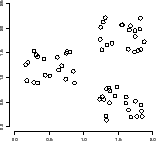
\includegraphics[scale=0.6]{pics/cluster.png}
\caption{Conjunto de documentos donde los grupos se pueden identificar claramente.}
\end{figure}

El clustering de documentos permite identificar tópicos en un corpus y reducir el espacio de búsqueda en un motor de búsqueda. Por ejemplo, el índice invertido se organiza según los grupos. El algoritmo K-means es una técnica de clustering simple que toma como parámetro el número de grupos, $k$.

El algoritmo se basa en la noción de \emph{centroides}, que son los vectores promedio de los documentos pertenecientes al mismo grupo. Por ejemplo, dado un conjunto de vectores bidimensionales $S = \{(3,6), (1,2), (5,1)\}$, el centroide de $S$ sería $(3,3)$, calculado como $(3+1+5)/3$ y $(6+2+1)/3$.

El algoritmo K-means comienza seleccionando $k$ centroides de manera aleatoria. Luego, calcula la similitud entre cada documento y cada centroide, asignando cada documento al centroide más cercano, formando así un grupo. Los centroides se recalculan de acuerdo con los documentos asignados a ellos. Este proceso se repite hasta que se cumple un criterio de convergencia, como se ilustra en el Algoritmo~\ref{algo:kmeans}.

\begin{algorithm}[H]
\SetKwInOut{Input}{Input}
\SetKwInOut{Output}{Output}
    \Input{Datos vectoriales $\vec{x}_1, \ldots, \vec{x}_N$ y el número de clusters $K$}
    \Output{centroides de clusters $\vec{\mu}_1, \ldots, \vec{\mu}_K$}
    $(\vec{s}_1, \vec{s}_2, \ldots, \vec{s}_K) \leftarrow$ SELECT\_RANDOM\_SEEDS($\vec{x}_1, \ldots, \vec{x}_N$, $K$)\;
    \For{$k \leftarrow 1$ \KwTo $K$}{
        $\vec{\mu}_k \leftarrow \vec{s}_k$\;
    }
    \While{no se cumpla el criterio de parada}{
        \For{$k \leftarrow 1$ \KwTo $K$}{
            $\omega_k \leftarrow \{\}$\;
        }
        \For{$n \leftarrow 1$ \KwTo $N$}{
            $j \leftarrow \arg\max_{j'} $coseno$(\vec{\mu}_{j'}, \vec{x}_n)$\;
            $\omega_j \leftarrow \omega_j \cup \{\vec{x}_n\}$\;
        }
        \For{$k \leftarrow 1$ \KwTo $K$}{
            $\vec{\mu}_k \leftarrow \frac{1}{{|\omega_k|}} \sum_{\vec{x} \in \omega_k} \vec{x}´$\;
        }
    }
    \Return{$\{\vec{\mu}_1, \ldots, \vec{\mu}_K\}$}\;
    \caption{K-Means}\label{algo:kmeans}
\end{algorithm}

\section{Conclusiones y Conceptos Adicionales}

En este capítulo, hemos explorado la representación de documentos como vectores para calcular similitudes entre ellos. Los vectores de ``bolsa-de-palabras'' son una forma común de representar documentos, pero tienen limitaciones ya que carecen de estructura lingüística y pueden ser de alta dimensionalidad y dispersos.

Una alternativa para capturar expresiones de múltiples palabras es utilizar n-gramas de palabras, que son secuencias contiguas de $n$ palabras. Por ejemplo, representar ``New York'' como ``new\_york'' nos permite capturar la relación entre esas dos palabras en lugar de tratarlas como entidades separadas.

Es importante señalar que los sistemas modernos de recuperación de información van más allá de la similitud de vectores. Utilizan algoritmos como PageRank \cite{page1998pagerank} para determinar la relevancia de un sitio web basándose en los enlaces que lo apuntan. También emplean técnicas de aprendizaje automático que utilizan registros de consultas anteriores para mejorar el ranking de resultados. Además, el uso de grafos de conocimiento enriquece aún más los resultados al proporcionar información estructurada y relaciones entre entidades.

Es importante destacar que disciplinas como la recuperación de información y la minería de textos se centran menos en la estructura lingüística que PLN y más en producir algoritmos rápidos y escalables para procesar grandes volúmenes de texto.



\chapter{Modelos de Lenguaje Probabilísticos}
\label{cap_plm}

En esta sección introducimos el concepto de ``modelo de lenguaje''. Un enfoque para asignar probabilidades a las oraciones que, como veremos a lo largo del apunte, desempeñará un papel fundamental en los enfoques modernos de PLN.

\section{El Problema del Modelado del Lenguaje}
Supongamos que tenemos un corpus de documentos $\mathcal{C}$, del cual extraemos su vocabulario (finito) a partir de la tokenización de sus documentos, $\mathcal{V} = \{$el, un, hombre, telescopio, Zamorano, dos, fan, vio, jugar, para, Real, Madrid, Zamorano, . . .$\}$.

Podemos formar a partir de este vocabulario un conjunto infinito de oraciones si dejamos que éstas sean de largo variable, $\mathcal{V}^*$. 

\begin{example}
Algunas oraciones que podríamos formar:
\begin{itemize}
\item el STOP
\item un STOP
\item el fan STOP
\item el fan vio a Zamorano STOP
\item el fan vio vio STOP
\item el fan vio a Zamorano jugar por el Real Madrid STOP
\end{itemize}

Donde STOP es un símbolo especial que indica el final de una oración.  
\end{example}

\begin{definition}
Un modelo de lenguaje es una distribución de probabilidad $p$ sobre todas las oraciones que se pueden formar a partir de un vocabulario finito. Entonces, la probabilidad de cada oración debe ser mayor o igual que cero, y la suma de las probabilidades de todas las oraciones posibles debe ser uno: 
\begin{align*}
\sum_{x\in V^*} p(x) &= 1 \\
p(x) &\geq 0 \quad \text{para todo } x \in V^*
\end{align*}
\end{definition}


\begin{example}
A continuación mostramos ejemplos de probabilidades asignadas por un modelo de lenguaje imaginario a algunas oraciones:
\begin{align*}
p(\text{el STOP}) &= 10^{-12} \\
p(\text{el fan STOP}) &= 10^{-8} \\
p(\text{el fan vio a Zamorano STOP}) &= 2 \times 10^{-8} \\
p(\text{el fan vio vio STOP}) &= 10^{-15} \\
\ldots \\
p(\text{el fan vio a Zamorano jugar por el Real Madrid STOP}) &= 2 \times 10^{-9}
\end{align*}
\end{example}



Lo que esperamos del modelo es que le asigne una probabilidad más alta a las oraciones fluidas (aquellas que tienen sentido y son gramaticalmente correctas) de las que no. También esperamos poder estimar esta función de probabilidad a partir del texto (corpus).

A nivel general, el modelo de lenguaje ayuda a los modelos de generación de texto a distinguir entre buenas y malas oraciones.


\subsection{¿Por qué querríamos hacer esto?}

La motivación original de estos modelos se origina en el problema de reconocimiento del habla o de transcripción automática para ayudar a estos sistemas a discernir entre disitntas oraciones compatibles con la señal acústica.  Consideremos las siguientes dos oraciones en inglés:
\begin{enumerate}
 \item ``recognize speech''  (reconocer el habla)
 \item ``wreck a nice beach'' (arruinar una playa bonita).
\end{enumerate}

Estas dos oraciones suenan muy similares al ser pronunciadas (tienen casi la misma señal acústica), lo que dificulta que los sistemas automáticos de reconocimiento del habla las transcriban con precisión. Cuando el sistema de reconocimiento del habla analiza la entrada de audio e intenta transcribirlo, tiene en cuenta las probabilidades del modelo de lenguaje para determinar la interpretación más probable.
El modelo de lenguaje favorecería $p$(``recognize speech'') sobre $p$(``wreck a nice beach'').
Esto se debe a que la primera oración es más común y debería ocurrir con más frecuencia en el corpus de entrenamiento.

Al incorporar modelos de lenguaje, los sistemas de reconocimiento del habla pueden mejorar  la precisión al seleccionar la oración que se alinea mejor con los patrones lingüísticos y el contexto, incluso cuando se enfrentan a alternativas que suenan similar.

De hecho, los modelos de lenguaje son útiles en cualquier tarea de procesamiento del lenguaje natural que involucre la generación de lenguaje (por ejemplo, traducción automática, resumen, generación de resúmenes, chatbots,  reconocimiento óptico de caracteres y el reconocimiento de escritura a mano).

Además la noción de modelamiento probabilístico del lenguaje se utiliza en muchos modelos y tareas de PLN, por lo que las técnicas de estimación desarrolladas en este capítulo serán muy útiles para entender muchos problemas en PLN.


\section{Regla de la Cadena en Modelos de Lenguaje}

En el contexto de los modelos de lenguaje, se parte de la premisa de que cualquier oración $s$ puede ser vista como una secuencia de variables aleatorias $X_1, X_2, \ldots, X_n$. Cada una de estas variables aleatorias puede tomar valores de un conjunto finito $V$. Para simplificar, asumimos una longitud fija $n$ para la secuencia. Nuestro objetivo consiste en modelar la probabilidad conjunta $p(X_1 = x_1, X_2 = x_2, \ldots, X_n = x_n)$. Es importante notar que utilizamos letras mayúsculas para denotar las variables aleatorias ($X_1, X_2, \ldots, X_n$) y minúsculas para referirnos a instancias específicas de estas variables ($x_1, x_2, \ldots, x_n$), que representan elementos del vocabulario (por ejemplo, ``perro'', ``gato'', ``comida'').

Una forma común de representar secuencias de variables aleatorias es mediante la aplicación de la regla de la cadena de probabilidades que definimos a continuación.

Para un conjunto de variables aleatorias $X_1,\ldots, X_n$, la regla de la cadena de probabilidades nos permite expresar la función de probabilidad conjunta $p(X_1,X_2,\ldots, X_n)$ como un producto de $n$ probabilidades condicionales:

\begin{equation}\label{eq:cadena}
p(X_1,X_2,\ldots,X_n)=p(X_1)p(X_2|X_1)p(X_3|X_2,X_1)\ldots p(X_n|X_{n-1},\ldots,X_2,X_1).
\end{equation}

Por ejemplo, en el caso de $n=3$, la expresión se simplifica a:

\begin{displaymath}
p(X_1,X_2,X_3)=p(X_1)p(X_2|X_1)p(X_3|X_2,X_1).
\end{displaymath}

Al utilizar la definición de probabilidades condicionales, podemos expresar $p(X_2|X_1)$ como $p(X_1,X_2)/p(X_1)$ y $p(X_3|X_2,X_1)$ como $p(X_1,X_2,X_3)/p(X_1,X_2)$. Al sustituir estas expresiones en la cadena de productos, vemos que todas las expresiones de cancelan y finalmente obtenemos $p(X_1,X_2,X_3)$.     

La aplicación de la regla de la cadena en los modelos de lenguaje no impone ningún supuesto específico sobre el modelo en sí. Más bien, nos proporciona una forma alternativa de modelar la probabilidad de una oración. Sin embargo, la ventaja de utilizar la regla de la cadena es que nos permite aplicar supuestos y hacer simplificaciones en el modelo para facilitar su implementación y cálculo.

\section{Mirada Predictiva}
La regla de la cadena nos permite darle una interpretación predictiva a los modelos de lenguaje. Uno puede asumir que un modelo de lenguaje una vez entrenado (o construido) a partir de un corpus es capaz de entregar una distribución de probabilidad para todas las palabras a partir de un contexto específico. Supongamos que tenemos un contexto formado por una secuencia de palabras $c=X_{n-1},\ldots,X_1$ y queremos predecir la palabra más probable a partir de ese contexto. Uno podría evaluar la probabilidad condicional $p(X_n|X_{n-1},\ldots,X_1)$ o $p(X_n|c)$ para todas las palabras del vocabulario que puede tomar $X_n$ y escoger la más probable:

\begin{displaymath}
x_n = \operatorname{argmax}_{X_n \in \mathcal{V}} p(X_n | c)
\end{displaymath}


\begin{example}
Supongamos que el contexto es $c=$``Cristóbal Colón descubrió''. El modelo de lenguaje sería capaz de determinar:

\begin{align*}
p(X|\text{``descubrió'', Colón'', ``Cristóbal''}) \\
\forall X \in V, \quad \text{donde} \sum_{X\in V}p(X|c)=1 
\end{align*}

Por ejemplo:

 
\begin{align*}
p(\text{``América''}|\text{``descrubrió'', ``Colón'', ``Cristóbal''}) = 0.02 \\
p(\text{``Europa''}|\text{``descrubrió'', ``Colón'', ``Cristóbal''}) = 0.01 \\
p(\text{``Chile''}|\text{``descrubrió'', ``Colón'', ``Cristóbal''}) = 0.001\\
p(\text{``camello''}|\text{``descrubrió'', ``Colón'', ``Cristóbal''}) = 0.00001 \\
\ldots
\end{align*}

Entonces, nuestro modelo de lenguaje predeciría $X=$``América'' como la palabra siguiente más probable.  
\end{example}

En el ejemplo anterior esperamos que un buen modelo de lenguaje asigne una probabilidad mayor a $X=$``América'' que al resto de las opciones. Para realizar estas predicciones, el modelo de lenguaje necesita capturar las reglas sintácticas y semánticas del lenguaje, así como tener un amplio conocimiento del mundo. 


Otra propiedad relevante, que se abordará en el Capítulo~\ref{cap_llm} sobre grandes modelos de lenguaje, es que se puede codificar prácticamente cualquier tarea de PLN como una instrucción dentro del contexto de un modelo de lenguaje. Por ejemplo, se podría utilizar la instrucción ``traduce el siguiente texto de inglés a español: I like dogs'', para luego esperar que el modelo de lenguaje sea capaz de realizar la traducción correcta.

\section{Mirada Generativa}

Los modelos de lenguaje aprendidos a partir de un corpus de texto no solo tienen una capacidad predictiva, sino que también tienen una capacidad generativa. Estos modelos pueden utilizarse para generar oraciones nuevas muestreando secuencialmente a partir de las probabilidades condicionales estimadas.

El proceso generativo implica tomar una palabra inicial y, a medida que avanzamos en la generación, seleccionar sucesivas palabras basadas en las probabilidades condicionales proporcionadas por el modelo de lenguaje. Es similar a extraer bolas (palabras) de una urna, donde los tamaños de las bolas están en proporción a sus frecuencias relativas, que son determinadas por el modelo de lenguaje. Cada vez que se selecciona una palabra, se utiliza como contexto para determinar la siguiente palabra, y así sucesivamente hasta que se haya generado una oración completa.

En este proceso generativo, hay diferentes enfoques que se pueden tomar. Uno de ellos es el muestreo estocástico, donde se elige una palabra de acuerdo con su probabilidad condicional dada por el modelo. Esto permite cierta variabilidad en la generación de oraciones, ya que las palabras menos probables también tienen la posibilidad de ser seleccionadas. Por otro lado, también se puede optar por seleccionar la palabra más probable en cada paso, lo que equivale a predecir la siguiente palabra basándose únicamente en la información disponible hasta ese momento. 


\section{Un Método Ingenuo}
Un método muy ingenuo para estimar la probabilidad de una oración es contar todas las apariciones de  oraciones idénticas a esta en los datos de entrenamiento y dividirlo por el número total de oraciones de entrenamiento ($N$).

Más formalmente, sea mi oración $s=x_1, x_2, \ldots, x_n$, y $c(x_1, x_2, \ldots, x_n)$  el número de veces que ocurre la oración en el corpus de entrenamiento, el modelo de lenguaje ingenuo computa la probabilidad de la siguiente manera: \begin{displaymath}
p(x_1,x_2,\cdots,x_n)=\frac{c(x_1,x_2 \dots,x_n)}{N}
\end{displaymath}

El problema de este enfoque, es que el número de posibles oraciones crece de manera exponencial con su cantidad de palabras y el tamaño del vocabulario. Entonces se vuelve cada vez más improbable que una oración específica haya ocurrido en los datos de entrenamiento. Esto es una consecuencia de la propiedad de \textbf{dispersión} del lenguaje planteada en el Capítulo~\ref{cap_intro}.

En consecuencia, muchas oraciones tendrán una probabilidad cero según el modelo ingenuo, lo que lleva a una mala generalización.

\section{Procesos de Markov}


Un proceso de Markov de primer orden asume que la probabilidad de que una variable aleatoria tome un valor depende únicamente del valor inmediatamente anterior en la secuencia. En el contexto del modelado del lenguaje, esto significa que la probabilidad de una palabra en una oración depende solo de la palabra anterior. Si aplicamos este supuesto a la regla de cadena de probabilidades, la probabilidad conjunta de una secuencia de palabras se simplifica en una multiplicación de probabilidades condicionales de las palabras sucesivas dado su palabra predecesora inmediata:

\begin{equation}
p(X_i = x_i|X_1 = x_1, \ldots, X_{i-1} = x_{i-1}) = p(X_i = x_i|X_{i-1} = x_{i-1})
\end{equation}




Un proceso de Markov de segundo orden amplía la suposición de Markov de primer orden y considera el valor de dos variables anteriores en la secuencia. En el modelado del lenguaje, esto significa que la probabilidad de una palabra en una oración depende de las dos palabras anteriores. La probabilidad conjunta de una secuencia de palabras se calcula multiplicando las probabilidades condicionales de las palabras sucesivas dado sus dos palabras predecesoras:

\begin{equation}
p(X_i = x_i|X_1 = x_1, \ldots, X_{i-2} = x_{i-2}, X_{i-1} = x_{i-1}) = p(X_i = x_i|X_{i-2} = x_{i-2}, X_{i-1} = x_{i-1})
\end{equation}


\subsection{Modelado de secuencias de longitud variable}

Si queremos modelar secuencias de longitud variable, podemos considerar que la longitud de la secuencia, $n$, también es una variable aleatoria. Una forma simple de abordar esto es siempre definir $X_n = \text{STOP}$, donde ``STOP'' es un símbolo especial que marca el final de la secuencia. Luego, podemos usar un proceso de Markov como antes para modelar la probabilidad conjunta de las palabras en la secuencia:

\[
p(X_1 = x_1, X_2 = x_2, \ldots, X_n = x_n) = \prod_{i=1}^{n} p(X_i = x_i|X_{i-2} = x_{i-2}, X_{i-1} = x_{i-1})
\]

Aquí, asumimos que $x_0 = x_{-1} = *$ por conveniencia, donde ``*'' es un símbolo especial de ``inicio'' de oración.

\section{Modelos de lenguaje de Trigramas}

Un n-grama es una secuencia contigua de $n$ palabras. Un modelo de lenguaje de trigrama (n-grama con $n=3$) acoge los supuestos de independencia del modelo de Markov de segundo orden que se discutió anteriormente. De esta forma permite expresar la probabilidad de una oración de la siguiente forma:
\begin{equation}
p(X_1,X_2,\ldots,X_n)=p(X_1)p(X_2|X_1)p(X_3|X_2,X_1)\ldots p(X_n|X_{n-1},X_{n-2}).
\end{equation}

Nótese que en vez de condicionar por todas las palabras anteriores como en la Ecuación~\ref{eq:cadena} aquí solo se condiciona por las dos palabras anteriores.


Los componentes que definen al modelo de lenguaje de trigrama se definen a continuación:

\begin{enumerate}
  \item Un vocabulario $V$, representado por un conjunto finito de palabras.
  \item Un parámetro escalar $q(w|u, v)$ para cada trigrama $u, v, w$, donde $w \in V \cup \{\text{STOP}\}$ y $u, v \in V \cup \{*\}$.
\end{enumerate}

Para cualquier oración $x_1 \ldots x_n$, donde $x_i \in V$ para $i = 1 \ldots (n-1)$ y $x_n = \text{STOP}$, la probabilidad de la oración según el modelo de lenguaje trigrama es:

\[
p(x_1 \ldots x_n) = \prod_{i=1}^{n} q(x_i|x_{i-2}, x_{i-1})
\]

Aquí, definimos $x_0 = x_{-1} = *$ como dos tokens especiales antes del inicio del oración para poder condicionar tanto la primera como la segunda palabra de una oración por sus dos palabras. A este tipo de transformaciones se les conoce en PLN como ``padding''.

Por ejemplo, para la oración ``el perro ladra STOP'', estimaríamos su probabilidad de la siguiente forma:
\[
p(\text{el perro ladra STOP}) = q(\text{el}|*, *) \times q(\text{perro}|*, \text{el}) \times q(\text{ladra}|\text{el}, \text{perro}) \times q(\text{STOP}|\text{perro}, \text{ladra})
\]

Ahora abordemos el problema de la estimación de los parámetros $q(w_i | w_{i-2}, w_{i-1})$ a partir de un corpus $\mathcal{C}$.

Una estimación natural es la ``estimación de máxima verosimilitud'' (MLE por sus siglas en inglés), donde se estiman los parámetros para maximizar la probabilidad de los datos de entrenamiento.

En el contexto de un modelo de trigrama, la estimación de cada parámetro proviene de distribuciones multinomiales, lo cual se traduce en el siguiente cálculo:

\[
q(w_i | w_{i-2}, w_{i-1}) = \frac{{\text{Count}(w_{i-2}, w_{i-1}, w_i)}}{{\text{Count}(w_{i-2}, w_{i-1})}}
\]

Esto requiere tokenizar el corpus de entrenamiento y guardar en una tabla los conteos de todos los trigramas (secuencias contiguas de 3 palabras) y bigramas (secuencias contiguas de dos palabras) encontrados.

Por ejemplo:
\[
q(\text{ladra} | \text{el, perro}) = \frac{{\text{Count}(\text{el, perro, ladra})}}{{\text{Count}(\text{el, perro})}}
\]




\section{Evaluación de un modelo de lenguaje: Perplejidad}

Un modelo de lenguaje efectivo se caracteriza por asignar probabilidades más altas a oraciones coherentes que a oraciones sin sentido. Para evaluar la calidad de un modelo de lenguaje, es esencial utilizar un corpus de prueba independiente diferente al corpus en el que fue entrenado. Esto nos permitirá verificar cómo generaliza el modelo a nuevas oraciones.  La evaluación cuantitativa de modelos de lenguaje nos permite comparar distintos tipos de modelos de lenguaje y seleccionar el modelo más apropiado.

Para evaluar un modelo de lenguaje utilizamos un corpus de prueba independiente, $\mathcal{C}_{\text{test}}$, que contiene $m$ oraciones: $s_1, s_2, s_3, ..., s_m$, y cuantificamos la probabilidad que el modelo asigna a estas oraciones. Para esto, calculamos la probabilidad total asignada por el modelo a las oraciones del corpus de prueba, lo cual se puede expresar más convenientemente mediante la probabilidad logarítmica\footnote{El logaritmo es una función monótona y permite llevar los productos a suma que evita problemas de underflow al trabajar con números pequeños.}:
\[
\log \left( \prod_{i=1}^{m} p(s_i) \right) = \sum_{i=1}^{m} \log p(s_i)
\]

La medida de evaluación estándar para modelos de lenguaje es la perplejidad (o perplexity), que se calcula de la siguiente manera:
\[
\text{Perplejidad} = 2^{-l} \quad \text{donde} \quad l = \frac{1}{M} \sum_{i=1}^{m} \log p(s_i)
\]

Donde $M$ es el número total de palabras en los datos de prueba.

La perplejidad es una métrica que favorece valores más bajos y tiene la propiedad de ser más fácil de interpretar que la probabilidad logarítmica, como se discutirá a continuación.


\subsection{Intuición sobre la perplejidad}

Supongamos que tenemos un vocabulario $V$, y $N = |V| + 1$, y un modelo de lenguaje ``uniforme'' que le asigna la misma probabilidad a todos los trigramas:
    \[
        q(w|u, v) = \frac{1}{N} \quad \text{para todo } w \in V \cup \{\text{STOP}\}, \text{ para todo } u, v \in V \cup \{*\}
    \]

La perplejidad de este modelo de lenguaje es $N$ tal como se demuestra a continuación.

Supongamos que tenemos $m$ oraciones de longitud $n$ en el corpus, y $M$ es la cantidad de tokens en el corpus, $M = m \cdot n$. Consideremos el logaritmo (base 2) de la probabilidad de una oración $s = w_1 w_2 \dots w_n$ bajo el modelo:
    \[
        \log p(s) = \log \prod_{i=1}^{n} q(w_i|w_{i-2}, w_{i-1}) = \sum_{i=1}^{n} \log q(w_i|w_{i-2}, w_{i-1})
    \]
Dado que cada parámetro $q(w_i|w_{i-2}, w_{i-1})$ es igual a $\frac{1}{N}$, tenemos:
    \[
        \log p(s) = \sum_{i=1}^{n} \log \frac{1}{N} = n \cdot \log \frac{1}{N} = -n \cdot \log N
    \]
    
    
    \[
        l =  \frac{1}{M} \sum_{i=1}^{m} \log p(s_i) = \frac{1}{M} \sum_{i=1}^{m} -n \cdot \log N  = \frac{1}{M} \cdot -m \cdot n \cdot \log N = - \log N 
    \]
    
            
Por lo tanto, la perplejidad está dada por:
    \[
        \text{Perplejidad} = 2^{-l} = 2^{-(- \log N)} = N
    \]

    
Esperamos entonces, que cualquier modelo de lenguaje que sea capaz de aprovechar la distribución de las palabaras (como un modelo de trigramas) tenga una perplejidad menor que el tamaño del vocabulario. En \cite{goodman2001bit}, donde $|V| = 50,000$, se presentan los siguientes resultados:

\begin{itemize}
        \item Modelo de trigramas: $p(x_1, \ldots, x_n) = \prod_{i=1}^n q(x_i | x_{i-2}, x_{i-1})$ \\
        Perplejidad = 74
        \item Modelo de bigramas: $p(x_1, \ldots, x_n) = \prod_{i=1}^n q(x_i | x_{i-1})$ \\
        Perplejidad = 137
        \item Modelo de unigramas: $p(x_1, \ldots, x_n) = \prod_{i=1}^n q(x_i)$ \\
        Perplejidad = 955
    \end{itemize}
    
Estos resultados muestran que la perplejidad disminuye a medida que aumentamos el nivel de contexto considerado en el modelo de lenguaje, lo que indica que los modelos con perplejidad más baja generalmente son más efectivos en la tarea de predicción del lenguaje. Sin embargo, como veremos a continuación, aumentar el tamaño del contexto no esta libre de problemas.   

\subsection{El trade-off entre sesgo y varianza}

Una limitación de los modelos de trigramas está relacionada con la dispersión del lenguaje, discutida en el Capítulo~\ref{cap_intro}. A grandes rasgos, si el tamaño del vocabulario es $N = |V|$, entonces el modelo tiene $N^3$ parámetros. Por ejemplo, si $N = 20,000$, habría $20,000^3 = 8 \times 10^{12}$ parámetros. Esta cantidad de parámetros es enorme y dificulta la estimación adecuada de todos ellos sin requerir un corpus de entrenamiento de tamaño enorme. Como resultado, puede surgir un problema de sobreajuste (overfitting) a los datos de entrenamiento. Por otro lado, modelos más simples, como un modelo de lenguaje de unigrama o de bigrama, no son capaces de modelar adecuadamente el contexto.

Este dilema es conocido en estadística y aprendizaje automático como el trade-off entre sesgo y varianza, que se refiere a la compensación entre la simplicidad del modelo y su capacidad para capturar la complejidad y variabilidad de los datos.

Los modelos más simples, como los modelos de n-gramas de orden inferior (unigramas, bigramas), tienen un sesgo más alto pero una varianza más baja. Estos modelos asumen independencia condicional entre las palabras y simplifican la estructura del lenguaje.

En contraste, los modelos más complejos, como modelos de n-gramas con $n>3$, tienen una varianza más alta pero un sesgo más bajo. Estos modelos pueden capturar relaciones más complejas entre las palabras, pero también son más propensos a sobreajustar los datos de entrenamiento y tener dificultades para generalizar a nuevas muestras.

Cuando se entrena un modelo de lenguaje con MLE, se maximiza la probabilidad de los datos de entrenamiento. Esto puede llevar a asignar probabilidades altas a secuencias específicas que aparecen en los datos de entrenamiento, incluso si esas secuencias son poco probables en la distribución real del lenguaje.

Como resultado, el modelo puede tener un rendimiento deficiente en datos de prueba que contienen secuencias diferentes a las del conjunto de entrenamiento. Esto se debe a que el modelo se ha sobreajustado a los datos de entrenamiento y ha capturado sus características específicas en lugar de aprender patrones más generales del lenguaje.

Para abordar el problema del sobreajuste en modelos de lenguaje, se utilizan diversas técnicas de regularización. Estas técnicas ayudan a controlar la varianza del modelo y mitigar el sobreajuste, permitiendo un mejor equilibrio entre el sesgo y la varianza y mejorando la generalización a nuevas muestras. A continuación, veremos dos técnicas de regularización para modelos de lenguaje: la interpolación lineal y los modelos de descuento.




\section{Interpolación Lineal}

La pricipal idea detrás de la técnica de interpolación lineal es combinar las distribuciones de probabilidad estimadas por modelos de n-gramas con las obtenidas a través de modelos de órdenes inferiores, como bigramas y unigramas. Esta estrategia ofrece la ventaja de incorporar información de n-gramas de órdenes más bajos, permitiendo abordar la indefinición de probabilidades en palabras no observadas durante el entrenamiento. Pues basta que una oración tenga un sólo trigrama no observado en entrenamiento para recibir una probabilidad de cero por el efecto multiplicativo de la regla de la cadena.

En el modelo interpolado, se ponderan linealmente tres modelos distintos:

\begin{enumerate}
    \item Modelo de trigramas: $q_{\text{ML}}(w_i | w_{i-2}, w_{i-1}) = \frac{{\text{Count}(w_{i-2}, w_{i-1}, w_i)}}{{\text{Count}(w_{i-2}, w_{i-1})}}$
    \item Modelo de bigramas: $q_{\text{ML}}(w_i | w_{i-1}) = \frac{{\text{Count}(w_{i-1}, w_i)}}{{\text{Count}(w_{i-1})}}$
    \item Modelo de unigramas: $q_{\text{ML}}(w_i) = \frac{{\text{Count}(w_i)}}{{\text{Count}(\# \text{tokens en el corpus})}}$.
\end{enumerate}

Cada parámetro $q(w_i | w_{i-2}, w_{i-1})$ se interpola de la siguiente manera:

\[
q(w_i | w_{i-2}, w_{i-1}) = \lambda_1 \cdot q_{\text{ML}}(w_i | w_{i-2}, w_{i-1}) + \lambda_2 \cdot q_{\text{ML}}(w_i | w_{i-1}) + \lambda_3 \cdot q_{\text{ML}}(w_i)
\]

Donde $\lambda_1$, $\lambda_2$, y $\lambda_3$ son hiper-parámetros que deben definirse manualmente y cumplir con las condiciones $\lambda_1 + \lambda_2 + \lambda_3 = 1$, y $\lambda_i \geq 0$ para todo $i$. Como podemos ver, con esta técnica abordamos el problema de indefinición de probabilidades en el modelo de trigramas, puesto que si se le quiere asignar probabilidad a un trigrama no observado durante entrenamiento, este no necesariamente indefine las probabilidades pues puede recurrir a las probabilidades de los bigramas y unigramas correspondientes.


Además, se puede demostrar que el modelo interpolado define adecuadamente una distribución de probabilidad (donde definimos $V' = V \cup \{\text{STOP}\}$):

\[
\begin{aligned}
    & \sum_{w \in V'} q(w | u, v) \\
    &= \sum_{w \in V'} [\lambda_1 \cdot q_{\text{ML}}(w | u, v) + \lambda_2 \cdot q_{\text{ML}}(w | v) + \lambda_3 \cdot q_{\text{ML}}(w)] \\
    &= \lambda_1 \sum_{w} q_{\text{ML}}(w | u, v) + \lambda_2 \sum_{w} q_{\text{ML}}(w | v) + \lambda_3 \sum_{w} q_{\text{ML}}(w) \\
    &= \lambda_1 + \lambda_2 + \lambda_3 = 1
\end{aligned}
\]

También es posible demostrar que $q(w | u, v) \geq 0$ para todas las palabras en $V'$, ya que es una suma ponderada de tres cantidades no negativas.



\subsection{Estimación de los Valores $\lambda$}
Para encontrar un valor adecuado de los hiper-parámetros $\lambda$ se suele reservar una parte del conjunto de entrenamiento como datos de \textit{validación}. Definimos $c'(w_1, w_2, w_3)$ como el número de veces que se observa el trigrama $(w_1, w_2, w_3)$ en el conjunto de validación. Elegimos $\lambda_1$, $\lambda_2$, $\lambda_3$ para maximizar:
    \[
    L(\lambda_1, \lambda_2, \lambda_3) = \sum_{w_1,w_2,w_3} c'(w_1, w_2, w_3) \log q(w_3 | w_1, w_2)
    \]
    sujetos a $\lambda_1 + \lambda_2 + \lambda_3 = 1$, y $\lambda_i \geq 0$ para todo $i$, donde
    \[
    q(w_i | w_{i-2}, w_{i-1}) = \lambda_1 \cdot q_{\text{ML}}(w_i | w_{i-2}, w_{i-1}) + \lambda_2 \cdot q_{\text{ML}}(w_i | w_{i-1}) + \lambda_3 \cdot q_{\text{ML}}(w_i)
    \]

Esto generalmente se hace buscando en una grilla de posibles valores de todos los hiper-parámetros. Nótese que maximizar $L(\lambda_1, \lambda_2, \lambda_3)$ es equivalente a minimizar la perplejidad en validación.


\section{Modelos de Descuento (Katz Back-Off)}

Los modelos de descuento representan una técnica alternativa a la interpolación con el propósito de mejorar la generalización del modelo de lenguaje a datos que difieren de los utilizados en el entrenamiento. Además, estos modelos ayudan a evitar la sobreestimación de conteos para n-gramas con baja frecuencia de aparición. La idea principal detrás de los modelos de descuento es redistribuir la probabilidad de los n-gramas observados hacia aquellos que no se han observado.

Para ilustrar estos modelos, consideremos un ejemplo utilizando los conteos de bigramas que comienzan con el unigrama ``la'' en un corpus, junto con sus estimaciones de máxima verosimilitud, que se presentan en la Tabla~\ref{tab:plm_ej}. Se puede notar que estas estimaciones tienden a sobrevalorar lo que se ha observado en el corpus y subestimar lo que no se ha observado.

\begin{table}[h]
    \centering
    \begin{tabular}{|l|l|l|}\hline
        \textbf{Frase} & \textbf{Conteo} & \textbf{$q_{\text{ML}}(w_i | w_{i-1})$} \\
        \hline
        la & 48 & \\
        la, gata & 15 & $15/48$ \\
        la, mujer & 11 & $11/48$ \\
        la, persona & 10 & $10/48$ \\
        la, plaza & 5 & $5/48$ \\
        la, actividad & 2 & $2/48$ \\
        la, tuerca & 1 & $1/48$ \\
        la, revista & 1 & $1/48$ \\
        la, tarde & 1 & $1/48$ \\
        la, ciudad & 1 & $1/48$ \\
        la, calle & 1 & $1/48$ \\ \hline
    \end{tabular}\caption{Ejemplo de conteos de bigramas}\label{tab:plm_ej}
\end{table}

Podemos definir los conteos ``descontados'' de la siguiente manera:

\[
\text{Conteo}^*(x) = \text{Conteo}(x) - \beta
\]

Donde $\beta$ es una constante que generalmente se encuentra entre 0 y 1, siendo un valor típico 0.5. Con $\beta=0.5$, los conteos se descuentan, es decir, se reduce la probabilidad de los datos observados, como se muestra en la Tabla~\ref{tab:plm_ej}.

\begin{table}[h]
    \centering
    \begin{tabular}{|l|l|l|l|}\hline
        \textbf{Frase} & \textbf{Conteo} & \textbf{Conteo}$\mathbf{^*(x)}$ & $\mathbf{q_{\text{BO}}(w_i | w_{i-1})}$ \\
        \hline
        la & 48 & & \\
        la, gata & 15 & 14.5 & $14.5/48$ \\
        la, mujer & 11 & 10.5 & $10.5/48$ \\
        la, persona & 10 & 9.5 & $9.5/48$ \\
        la, plaza & 5 & 4.5 & $4.5/48$ \\
        la, actividad & 2 & 1.5 & $1.5/48$ \\
        la, tuerca & 1 & 0.5 & $0.5/48$ \\
        la, revista & 1 & 0.5 & $0.5/48$ \\
        la, tarde & 1 & 0.5 & $0.5/48$ \\
        la, ciudad & 1 & 0.5 & $0.5/48$ \\
        la, calle & 1 & 0.5 & $0.5/48$ \\\hline
    \end{tabular}\caption{Ejemplo de conteos de bigramas con conteos descontados}\label{tab:plm_ej}
\end{table}

Las nuevas estimaciones se basan en los conteos descontados, y se introduce una ``masa de probabilidad faltante'' como se muestra a continuación:

\[
\alpha(w_{i-1}) = 1 - \sum_{w} \frac{\text{Conteo}^*(w_{i-1}, w)}{\text{Conteo}(w_{i-1})}
\]

Por ejemplo, en nuestro caso:

\[
\alpha(\text{la}) = 1 - \frac{14.5+10.5+9.5+4.5+1.5+0.5+0.5+0.5+0.5+0.5}{48} = 1-\frac{43}{48} = \frac{5}{48}
\]

La idea es redistribuir esta masa faltante entre todos los bigramas que comienzan con la palabra ``la'' y que no fueron observados en el corpus, como por ejemplo ``rana'', ``bailarina'' y ``puerta''.

En el modelo de Katz Back-Off de bigramas, se definen dos conjuntos: $A(w_{i-1})$ y $B(w_{i-1})$, como se detalla a continuación:

\[
A(w_{i-1}) = \{w : \text{Count}(w_{i-1}, w) > 0\}
\]

En nuestro ejemplo, $A(\text{la}) = \{$ gata, mujer, persona, plaza, actividad, tuerca, revista, tarde, ciudad, calle $\}$.

Por otro lado, $B(w_{i-1})$ se define como:

\[
B(w_{i-1}) = \{w : \text{Count}(w_{i-1}, w) = 0\}
\]

En nuestro ejemplo, $B(\text{la}) = \{$ rana, bailarina, puerta, $\dots$ $\}$.

Luego, la probabilidad condicional $q_{\text{BO}}(w_i | w_{i-1})$ se calcula de la siguiente manera: si la palabra $w_i$ está en el conjunto $A(w_{i-1})$, se utiliza una estimación basada en las frecuencias relativas de la secuencia $(w_{i-1}, w_i)$ dividida por la frecuencia de $w_{i-1}$. Si $w_i$ está en el conjunto $B(w_{i-1})$, se utiliza una estimación suavizada que combina la constante $\alpha(w_{i-1})$ y las probabilidades condicionales de máxima verosimilitud  de un modelo orden inferior (unigramas) $q_{\text{ML}}(w_i)$ de las palabras en el conjunto $B(w_{i-1})$. Esta última ponderación asegura que las probabilidades queden bien definidas.

\[
q_{\text{BO}}(w_i | w_{i-1}) =
\begin{cases}
    \frac{\text{Count}^*(w_{i-1}, w_i)}{\text{Count}(w_{i-1})} & \text{si } w_i \in A(w_{i-1}) \\
    \frac{\alpha(w_{i-1}) q_{\text{ML}}(w_i)}{\sum_{w \in B(w_{i-1})} q_{\text{ML}}(w)} & \text{si } w_i \in B(w_{i-1})
\end{cases}
\]

La constante $\alpha(w_{i-1})$ se calcula restando la suma de las frecuencias relativas de las palabras en $A(w_{i-1})$ de uno tal como se definió anteriormente.



Para extender este enfoque a trigramas, se definen conjuntos similares $A(w_{i-2}, w_{i-1})$ y $B(w_{i-2}, w_{i-1})$ para las secuencias de trigramas:

\[
A(w_{i-2}, w_{i-1}) = \{w : \text{Count}(w_{i-2}, w_{i-1}, w) > 0\}
\]
\[
B(w_{i-2}, w_{i-1}) = \{w : \text{Count}(w_{i-2}, w_{i-1}, w) = 0\}
\]

La probabilidad condicional $q_{\text{BO}}(w_i | w_{i-2}, w_{i-1})$ en un modelo de trigramas se calcula utilizando el modelo de bigrama correspondiente y aplicando la misma lógica anterior:

\[
q_{\text{BO}}(w_i | w_{i-2}, w_{i-1}) =
\begin{cases}
    \frac{\text{Count}^*(w_{i-2}, w_{i-1}, w_i)}{\text{Count}(w_{i-2}, w_{i-1})} & \text{si } w_i \in A(w_{i-2}, w_{i-1}) \\
    \frac{\alpha(w_{i-2}, w_{i-1}) q_{\text{BO}}(w_i|w_{i-1})}{\sum_{w \in B(w_{i-2}, w_{i-1})} q_{\text{BO}}(w|w_{i-1})} & \text{si } w_i \in B(w_{i-2}, w_{i-1})
\end{cases}
\]

Donde:

\[
\alpha(w_{i-2}, w_{i-1}) = 1 - \sum_{w \in A(w_{i-2}, w_{i-1})} \frac{\text{Count}^*(w_{i-2}, w_{i-1}, w)}{\text{Count}(w_{i-2}, w_{i-1})}
\]

Estos modelos de Katz Back-Off ofrecen una aproximación efectiva de las probabilidades condicionales en situaciones en las que la información disponible es limitada, al aprovechar la información de contextos más pequeños cuando no se dispone de suficientes datos para estimaciones directas.

\section{Historia}
En 1951, mientras trabajaba en los laboratorios Bell, Claude Shannon (en la Figura~\ref{fig:shannon}) realizó experimentos sobre la entropía del inglés, modelando el lenguaje escrito de manera estadística y predictiva \cite{shannon1951prediction}. Utilizando modelos de lenguaje de n-gramas, Shannon exploró la dificultad de predecir palabras basándose en las palabras anteriores.

\begin{figure}[h]
    \centering
    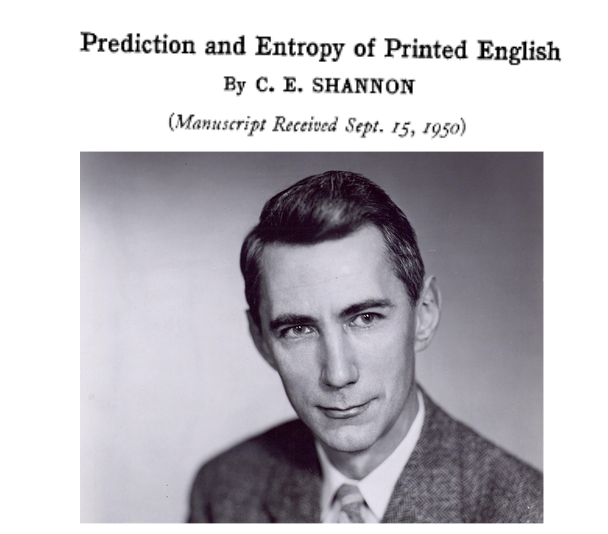
\includegraphics[scale = 0.4]{pics/shannon.png}
    \caption{Imagen de Shannon.}
    \label{fig:shannon}
\end{figure}

Por otro lado, en su libro \textit{Syntactic Structures} (1957), Noam Chomsky (en la Figura~\ref{fig:chomsky}), un lingüista y científico cognitivo, cuestionó la capacidad de los modelos de lenguaje probabilísticos para capturar y comprender la gramática del lenguaje humano \cite{chomsky2009syntactic}. Según Chomsky, la noción de ``gramaticalmente correcto'' no puede ser equiparada a ``significativo'' en un sentido probabilista. Para ilustrar esto, presentó dos oraciones ficticias, ambas carentes de sentido:

\begin{enumerate}
    \item Colorless green ideas sleep furiously.
    \item Furiously sleep ideas green colorless.
\end{enumerate}

Aunque ambas oraciones carecen de significado, Chomsky argumentó que solo la primera se considera gramaticalmente correcta por los hablantes de inglés. Además, enfatizó que la corecctitud gramatical en inglés no puede determinarse únicamente mediante aproximaciones estadísticas. Aunque es poco probable que ninguna de las dos oraciones (1) o (2) haya surgido en documentos escritos en inglés, un modelo estadístico como los modelos de lenguaje vistos en este capítulo las consideraría igualmente ``remotas'' en relación al inglés. Sin embargo, la oración (1) es gramaticalmente correcta, mientras que la oración (2) no lo es, lo que destaca las limitaciones de los enfoques estadísticos para capturar la gramática. Estos argumentos retrasaron el estudio de los modelos de lenguaje probabilísticos durante varios años \cite{JurafskyBook}.

\begin{figure}[h]
    \centering
    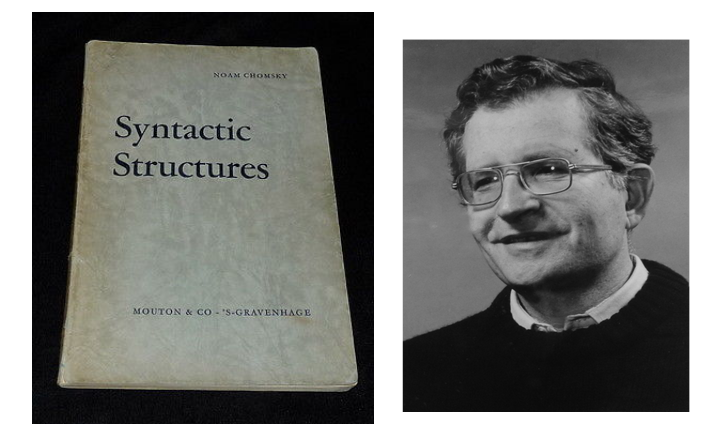
\includegraphics[scale = 0.4]{pics/chomsky.png}
    \caption{Imagen de Chomsky}
    \label{fig:chomsky}
\end{figure}


\section{Conclusiones}
El cálculo de probabilidades en modelos de lenguaje probabilísticos implica tres pasos:
    \begin{enumerate}
        \item Expandir $p(w_1, w_2, \ldots, w_n)$ usando la regla de la Cadena.
        \item Aplicar los supuestos Independencia de Markov \\
        $p(w_i | w_1, w_2, \ldots, w_{i-2}, w_{i-1}) = p(w_i | w_{i-2}, w_{i-1})$.
        \item Suavizar las estimaciones utilizando conteos de orden inferior.
    \end{enumerate}

No obstante, los modelos de lenguaje de bigramas o trigramas (que consideran dos palabras anteriores como contexto) tienen limitaciones en contextos largos y no pueden aprovechar contextos similares. Por ejemplo, consideremos los contextos:
\begin{itemize}
 \item $c_1$: Después de comer cereales
\item  $c_2$: Luego de desayunar avena
\end{itemize}

Aunque esperaríamos que las distribuciones de probabilidad $p(w|c_1)$ y $p(w|c_2)$ fueran similares, dado que $c_1$ y $c_2$ casi no comparten palabras, los modelos de n-gramas que se limitan a contar frecuencia de palabras no pueden capturar estas similitudes entre contextos.


Otros métodos para mejorar los modelos de lenguaje incluyen introducir variables latentes para representar tópicos, conocidos como modelos de tópicos \cite{blei2003latent} presentados en el Capítulo~\ref{cap_ir}. O alternativamente, reemplazar $p(w_i | w_1, w_2, \ldots, w_{i-2}, w_{i-1})$ con una red neuronal predictiva y una ``capa de embedding'' para representar mejor contextos más grandes y aprovechar similitudes entre palabras en el contexto. \cite{bengio2000neural}

Los modelos de lenguaje modernos utilizan redes neuronales profundas en su estructura principal y tienen un vasto espacio de parámetros como se verá en el Capítulo~\ref{cap_llm}.





\chapter{Text Classification and Naïve Bayes}
\label{cap_nb}
\begin{itemize}
    \item La clasificación es fundamental tanto para la inteligencia humana como para la artificial.
    \item Decidir qué letra, palabra o imagen se ha presentado a nuestros sentidos, reconocer caras o voces, clasificar el correo, asignar calificaciones a las tareas.
    \item Estos son ejemplos de asignar una categoría a una entrada.
    \item El objetivo de la clasificación es tomar una única observación, extraer algunas características útiles y así clasificar la observación en una de las clases discretas establecidas.
    \item La mayoría de los casos de clasificación en el procesamiento del lenguaje se realizan mediante aprendizaje automático supervisado.
    \item Estas diapositivas se basan en el material del curso de Daniel Jurafsky: \url{https://web.stanford.edu/~jurafsky/slp3/4.pdf}
\end{itemize}

Ejemplo 1: Clasificación de spam

\begin{figure}[h]
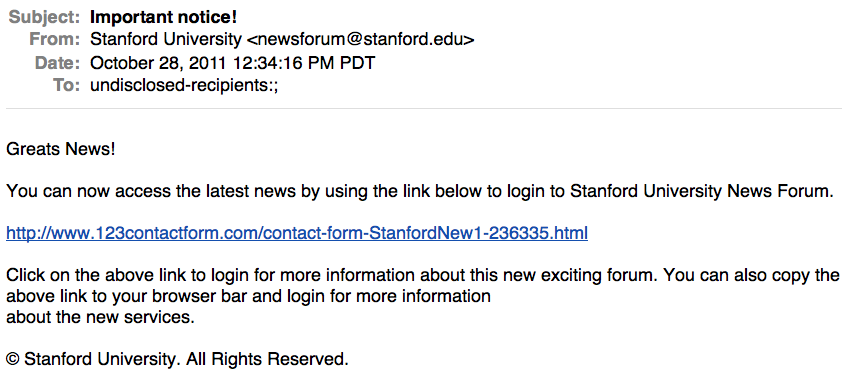
\includegraphics[scale = 0.35]{pics/spam.png}
\end{figure}


Ejemplo 2: ¿Quién escribió los documentos Federalist?

\begin{itemize}
    \item 1787-8: Ensayos anónimos intentaron convencer a Nueva York de ratificar la Constitución de EE. UU.: Jay, Madison, Hamilton.
    \item La autoría de 12 de las cartas está en disputa.
    \item 1963: Resuelto por Mosteller y Wallace mediante métodos bayesianos.
\end{itemize}

\begin{center}
    \begin{figure}[h]
        \begin{minipage}{0.3\textwidth}
            \centering
            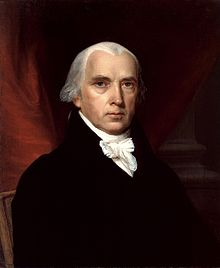
\includegraphics[width=\linewidth]{pics/madison.png}
            \caption{James Madison}
        \end{minipage}\hfill
        \begin{minipage}{0.3\textwidth}
            \centering
            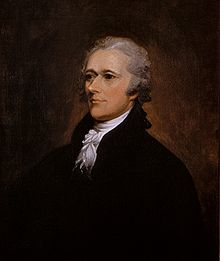
\includegraphics[width=\linewidth]{pics/hamilton.png}
            \caption{Alexander Hamilton}
        \end{minipage}
    \end{figure}
\end{center}


Ejemplo 3: ¿Cuál es el tema de este artículo médico?

\begin{figure}[h]
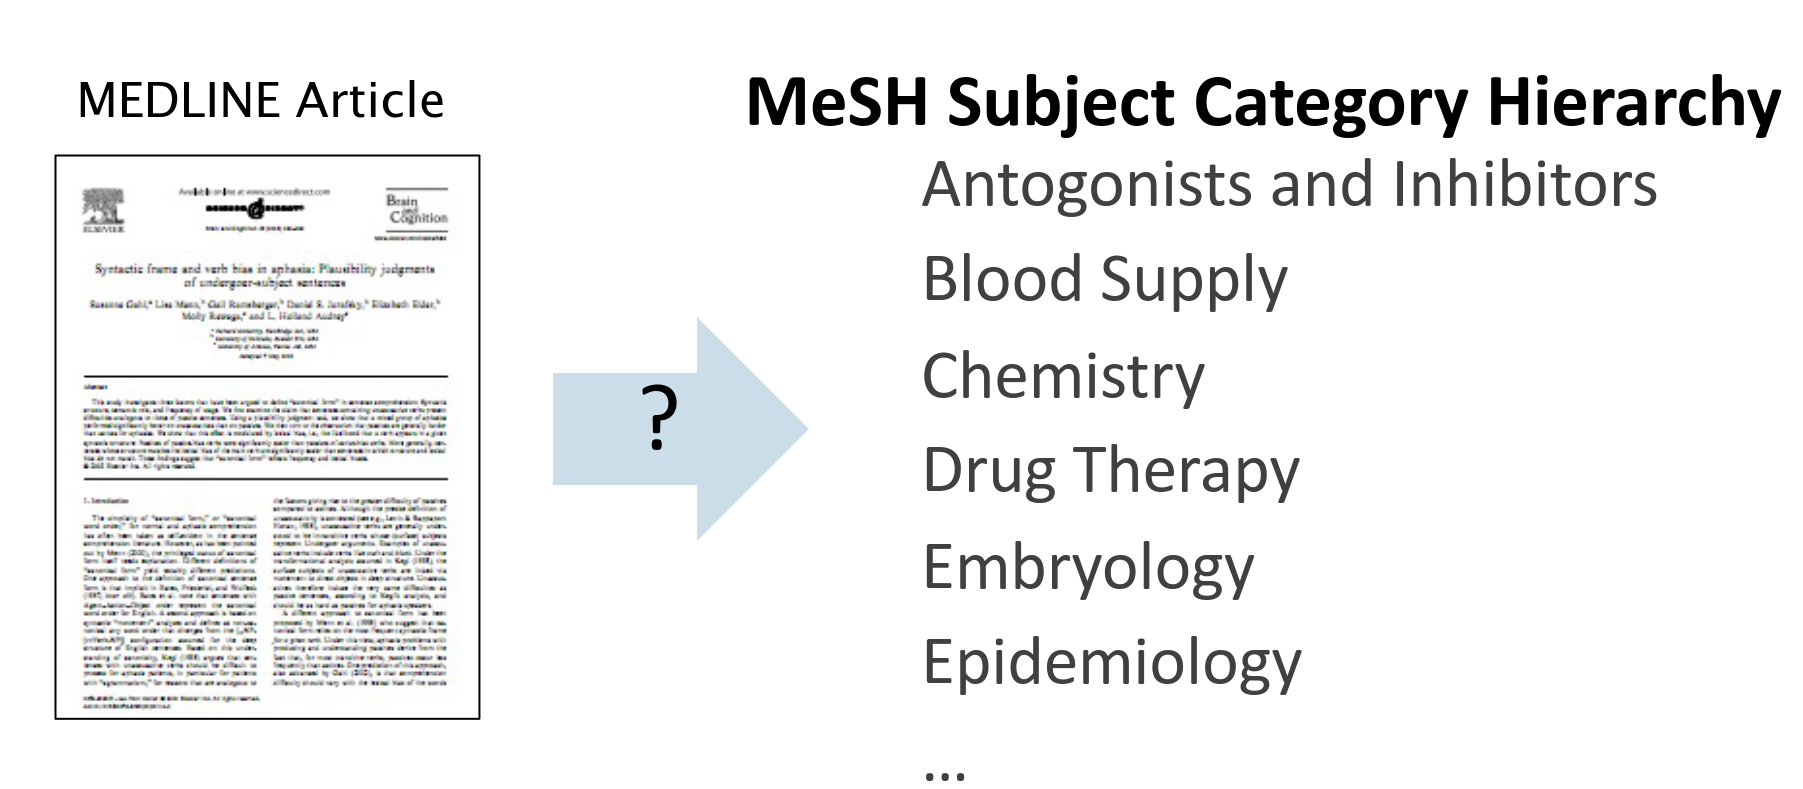
\includegraphics[scale = 0.2]{pics/medarticle.png}
\end{figure}



Ejemplo 4: ¿Reseña de película positiva o negativa?

\begin{itemize}
    \item \textcolor{blue}{\textbf{+}} ...personajes extravagantes y sátira \textcolor{blue}{rico} aplicada, y algunos \textcolor{blue}{grandes} giros de la trama.
    \item \textcolor{red}{\textbf{-}} Fue \textcolor{red}{patético}. La peor parte fue las escenas de boxeo...
    \item \textcolor{blue}{\textbf{+}} ...salsa de caramelo \textcolor{blue}{increíble} y almendras dulces y tostadas. ¡Me \textcolor{blue}{encanta} este lugar!
    \item \textcolor{red}{\textbf{-}} ...pizza \textcolor{red}{horrible} y \textcolor{red}{ridículamente} cara...
\end{itemize}



\paragraph{¿Por qué el análisis de sentimientos?}

\begin{itemize}
    \item Película: ¿Esta reseña es positiva o negativa?
    \item Productos: ¿Qué opinan las personas sobre el nuevo iPhone?
    \item Sentimiento público: ¿Cómo está la confianza del consumidor?
    \item Política: ¿Qué opinan las personas sobre este candidato o tema?
    \item Predicción: Predecir resultados electorales o tendencias del mercado a partir del sentimiento.
\end{itemize}


\paragraph{Clasificación básica de sentimientos}

El análisis de sentimientos es la detección de actitudes.

\begin{itemize}
    \item Tarea simple en la que nos enfocamos en esta clase.
    \begin{itemize}
        \item ¿Es la actitud de este texto positiva o negativa?
    \end{itemize}
\end{itemize}



\paragraph{Resumen: Clasificación de texto}

La clasificación de texto se puede aplicar a varias tareas, incluyendo:

\begin{itemize}
    \item Análisis de sentimientos
    \item Detección de spam
    \item Identificación de autoría
    \item Identificación de idioma
    \item Asignación de categorías, temas o géneros
    \item ...
\end{itemize}


\section{Clasificación de texto: Definición}

\textbf{Entrada}:
\begin{itemize}
    \item Un documento $d$
    \item Un conjunto fijo de clases $C = \{c_1, c_2, \ldots, c_J\}$
\end{itemize}

\textbf{Salida}: Una clase predicha $c \in C$


\subsection{Métodos de clasificación: Reglas codificadas a mano}

Reglas basadas en combinaciones de palabras u otras características.

\begin{itemize}
    \item Spam: \textit{dirección-en-lista-negra} O (\textit{“dólares” Y “has sido seleccionado”})
    \item La precisión puede ser alta si las reglas se refinan cuidadosamente por expertos
    \item Pero construir y mantener estas reglas es costoso
\end{itemize}

\subsection{Métodos de clasificación: Aprendizaje automático supervisado}

\textbf{Entrada}:
\begin{itemize}
    \item Un documento $d$
    \item Un conjunto fijo de clases $C = \{c_1, c_2, \ldots, c_J\}$
    \item Un conjunto de entrenamiento de $m$ documentos etiquetados manualmente: $(d_1, c_1), (d_2, c_2), \ldots, (d_m, c_m)$
\end{itemize}

\textbf{Salida}:
\begin{itemize}
    \item Un clasificador aprendido $\gamma: d \to c$
\end{itemize}

Cualquier tipo de clasificador se puede utilizar:
\begin{itemize}
    \item Naïve Bayes
    \item Regresión logística
    \item Redes neuronales
    \item k-vecinos más cercanos
    % Agrega más clasificadores según sea necesario
\end{itemize}

\subsection{Problemas de aprendizaje supervisado}
\begin{itemize}
    \item Tenemos ejemplos de entrenamiento $x^{(i)}$, $y^{(i)}$ para $i = 1, \ldots, m$. Cada $x^{(i)}$ es una entrada, cada $y^{(i)}$ es una etiqueta.
    \item La tarea es aprender una función $f$ que asigna las entradas $x$ a las etiquetas $f(x)$.
    \item Modelos condicionales:
    \begin{itemize}
        \item Aprender una distribución $p(y|x)$ a partir de ejemplos de entrenamiento.
        \item Para cualquier entrada de prueba $x$, definir $f(x) = \arg \max_y p(y|x)$.
    \end{itemize}
\end{itemize}

\subsection{Modelos generativos}
\begin{itemize}
    \item Dados ejemplos de entrenamiento $x^{(i)}$, $y^{(i)}$ para $i = 1, \ldots, m$, la tarea es aprender una función $f$ que asigna las entradas $x$ a las etiquetas $f(x)$.
    \item Modelos generativos:
    \begin{itemize}
        \item Aprender la distribución conjunta $p(x, y)$ a partir de los ejemplos de entrenamiento.
        \item A menudo, tenemos $p(x, y) = p(y)p(x|y)$.
        \item Nota: Luego tenemos
        \[
        p(y|x) = \frac{p(y)p(x|y)}{p(x)} \quad \text{donde} \quad p(x) = \sum_y p(y)p(x|y).
        \]
    \end{itemize}
\end{itemize}

\subsection{Clasificación con Modelos Generativos}
\begin{itemize}
    \item Dados ejemplos de entrenamiento $x^{(i)}$, $y^{(i)}$ para $i = 1, \ldots, m$. La tarea consiste en aprender una función $f$ que mapee las entradas $x$ a las etiquetas $f(x)$.
    \item Modelos generativos:
    \begin{itemize}
        \item Aprenden la distribución conjunta $p(x, y)$ a partir de los ejemplos de entrenamiento.
        \item A menudo, tenemos $p(x, y) = p(y)p(x|y)$.
    \end{itemize}
    \item La salida del modelo es:
    \[
    \begin{aligned}
    f(x) = \arg\max_y p(y|x) &= \arg\max_y \frac{p(y)p(x|y)}{p(x)} \\
    &= \arg\max_y p(y)p(x|y)
    \end{aligned}
    \]
\end{itemize}


\section{Intuición del Bayes Ingenuo}
El Bayes Ingenuo es un método de clasificación simple ("ingenuo") basado en la regla de Bayes.
\begin{itemize}
    \item Se basa en una representación muy simple de un documento: \textit{Bolsa de palabras}.
\end{itemize}

\paragraph{La Representación de Bolsa de Palabras}

\begin{figure}[h]
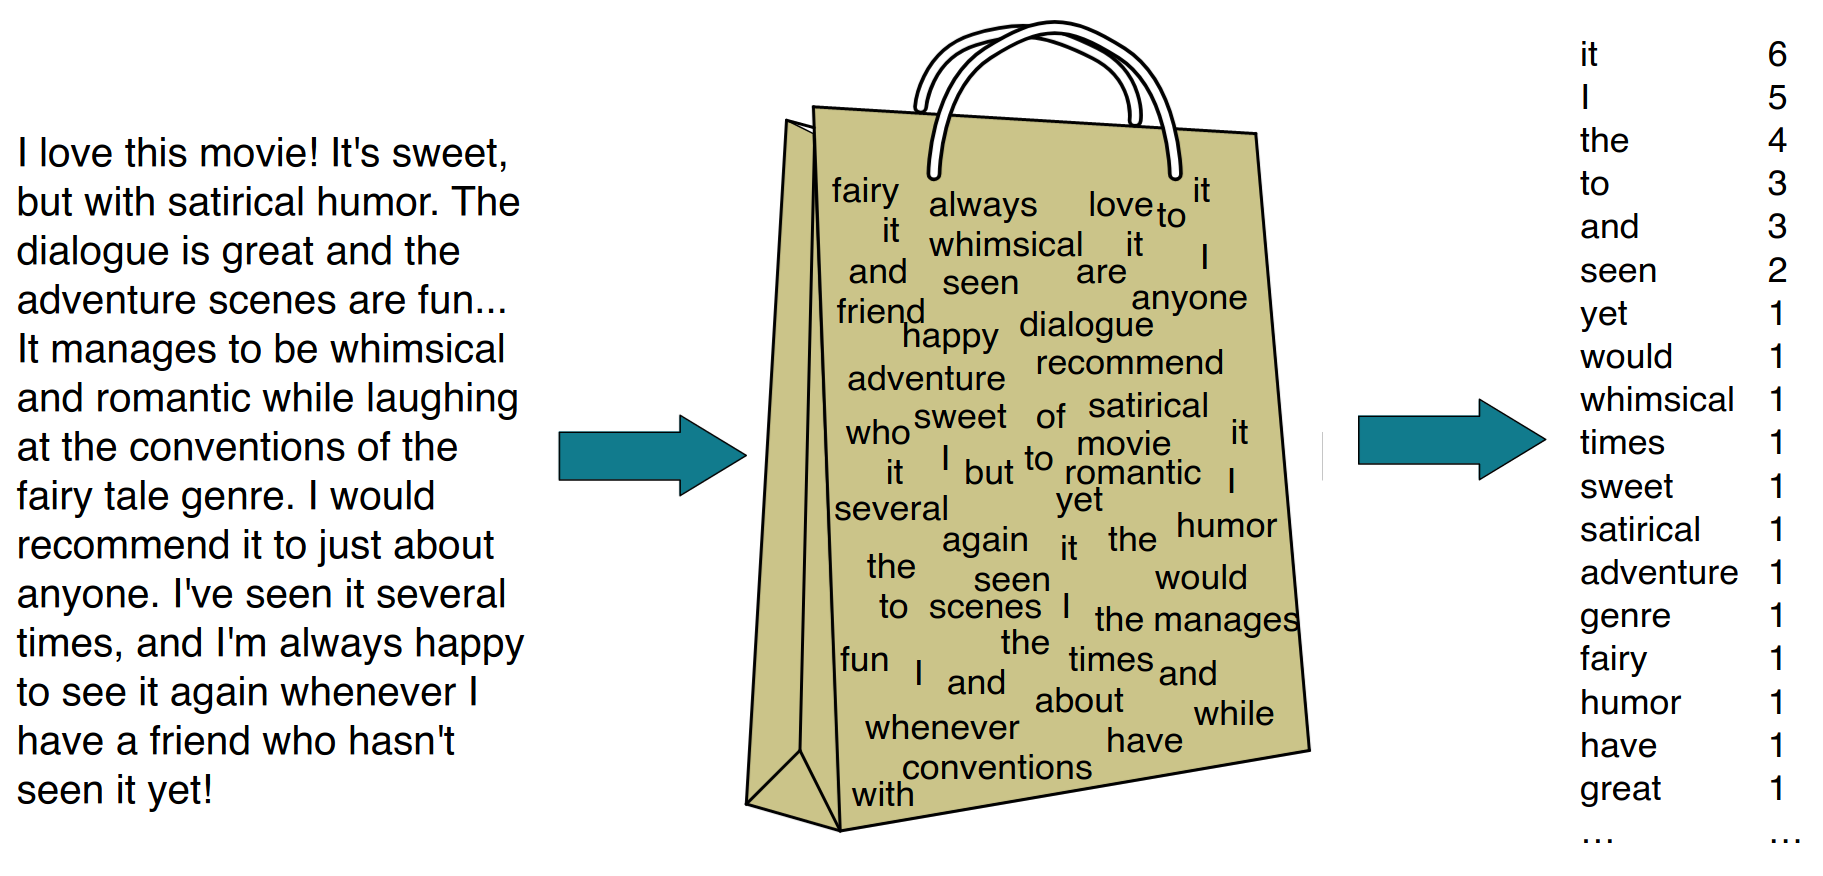
\includegraphics[scale = 0.22]{pics/bow.png}
\end{figure}


\subsection{Aplicación de la Regla de Bayes a Documentos y Clases}
Para un documento $d$ y una clase $c$:
\[
P(c | d) = \frac{P(d | c)P(c)}{P(d)}
\]


\section{Clasificador Bayes Ingenuo}
\begin{itemize}
    \item MAP significa ``máximo a posteriori'', que representa la clase más probable:
    \[
    c_{\text{MAP}} = \arg\max_{c \in C} P(c | d)
    \]
    \item Para calcular la clase más probable, aplicamos la regla de Bayes:
    \[
    = \arg\max_{c \in C} \frac{P(d | c)P(c)}{P(d)}
    \]
    \item Finalmente, podemos eliminar el denominador ya que permanece constante para todas las clases:
    \[
    = \arg\max_{c \in C} P(d | c)P(c)
    \]
    \item Para clasificar el documento $d$, usamos la estimación MAP:
    \[
    c_{\text{MAP}} = \arg\max_{c \in C} P(d | c)P(c)
    \]
    \item El documento $d$ se representa como un conjunto de características $x_1, x_2, \ldots, x_n$.
    \item El clasificador calcula la probabilidad condicional de las características dada una clase y la probabilidad a priori de la clase:
    \[
    = \arg\max_{c \in C} P(x_1, x_2, \ldots, x_n | c)P(c)
    \]
    \item El término $P(x_1, x_2, \ldots, x_n | c)$ representa la

 "verosimilitud" de las características dada la clase.
    \item El término $P(c)$ representa la probabilidad "a priori" de la clase.
    \item El clasificador Bayes Ingenuo \cite{mccallum1998comparison} calcula la estimación MAP considerando las probabilidades de verosimilitud y a priori:
    \[
    c_{\text{MAP}} = \arg\max_{c \in C} P(x_1, x_2, \ldots, x_n | c)P(c)
    \]
    \item La probabilidad de las características dada la clase, $P(x_1, x_2, \ldots, x_n | c)$, puede estimarse contando las frecuencias relativas en un corpus.
    \item La probabilidad a priori de la clase, $P(c)$, representa con qué frecuencia ocurre esta clase.
    \item Sin algunas suposiciones simplificadoras, estimar la probabilidad de cada posible combinación de características en $P(x_1, x_2, \ldots, x_n | c)$ requeriría un gran número de parámetros y conjuntos de entrenamiento imposiblemente grandes.
    \item Por lo tanto, los clasificadores Bayes Ingenuo realizan dos suposiciones simplificadoras.
\end{itemize}


\subsection{Suposiciones de Independencia del Bayes Ingenuo Multinomial}
\begin{itemize}
    \item Suposición de Bolsa de Palabras: asumimos que la posición de las palabras en el documento no importa.
    \item Suposición de Independencia Condicional: asumimos que las probabilidades de las características $P(x_i | c_j)$ son independientes dada la clase $c_j$.
    \item En el clasificador Bayes Ingenuo Multinomial, la probabilidad de un documento con características $x_1, x_2, \ldots, x_n$ dada la clase $c$ se puede calcular como:
    \[
    P(x_1, x_2, \ldots, x_n | c) = P(x_1 | c) \cdot P(x_2 | c) \cdot P(x_3 | c) \cdot \ldots \cdot P(x_n | c)
    \]
\end{itemize}

\subsection{Clasificador Bayes Ingenuo Multinomial}
\begin{itemize}
    \item La estimación del Máximo A Posteriori (MAP) para la clase $c$ en el clasificador Bayes Ingenuo Multinomial se calcula como:
    \[
    c_{\text{MAP}} = \arg\max_{c \in C} P(x_1, x_2, \ldots, x_n | c)P(c)
    \]
    \item Alternativamente, podemos escribirlo como:
    \[
    c_{\text{NB}} = \arg\max_{c \in C} P(c_j) \prod_{x \in X} P(x | c)
    \]
    \item $P(c_j)$ representa la probabilidad a priori de la clase $c_j$.
    \item $\prod_{x \in X} P(x | c)$ representa la verosimilitud de las características $x_1, x_2, \ldots, x_n$ dadas la clase $c$.
\end{itemize}


\subsection{Aplicación de los clasificadores Naive Bayes multinomiales a la clasificación de texto}

El clasificador Naive Bayes multinomial para la clasificación de texto se puede aplicar de la siguiente manera:
\[
c_{\text{NB}} = \arg\max_{c_j \in C} P(c_j) \prod_{i \in \text{positions}} P(x_i | c_j)
\]
Donde:
\begin{itemize}
    \item $c_{\text{NB}}$ representa la clase predicha para el documento de prueba.
    \item $C$ es el conjunto de todas las clases posibles.
    \item $P(c_j)$ es la probabilidad previa de la clase $c_j$.
    \item $\prod_{i \in \text{positions}} P(x_i | c_j)$ calcula la probabilidad de cada característica $x_i$ en la posición $i$ dada la clase $c_j$.
    \item El producto se toma sobre todas las posiciones de palabras en el documento de prueba.
\end{itemize}

\subsection{Problemas al multiplicar muchas probabilidades}

Multiplicar muchas probabilidades puede resultar en un desbordamiento de punto flotante, especialmente cuando se manejan probabilidades pequeñas. Por ejemplo, $0.0006 \times 0.0007 \times 0.0009 \times 0.01 \times 0.5 \times 0.000008 \ldots$.

Para solucionar este problema, podemos utilizar logaritmos, ya que $\log(ab) = \log(a) + \log(b)$. En lugar de multiplicar las probabilidades, podemos sumar los logaritmos de las probabilidades. Así, el clasificador Naive Bayes multinomial se puede expresar utilizando logaritmos de la siguiente manera:
\[
c_{\text{NB}} = \arg\max_{c_j \in C} \left(\log(P(c_j)) + \sum_{i \in \text{position}} \log(P(x_i | c_j))\right)
\]

Al tomar logaritmos, evitamos el problema del desbordamiento de punto flotante y realizamos cálculos en el espacio logarítmico. El clasificador se convierte en un modelo lineal, donde la predicción es el argmax de la suma de pesos (logaritmos de probabilidades) y las entradas (logaritmos de probabilidades condicionales). Por lo tanto, Naive Bayes es un clasificador lineal que opera en el espacio logarítmico.

\subsection{Aprendizaje del modelo Naive Bayes multinomial}

El primer intento: Estimaciones de máxima verosimilitud
\begin{itemize}
    \item Las probabilidades se estiman utilizando las frecuencias observadas en los datos de entrenamiento.
    \item La probabilidad previa de una clase $c_j$ se estima como:
    \[
    \hat{P}(c_j) = \frac{N_{c_j}}{N_{\text{total}}}
    \]
    donde $N_{c_j}$ es el número de documentos en la clase $c_j$ y $N_{\text{total}}$ es el número total de documentos.
    \item La estimación de la probabilidad de la palabra $w_i$ dada la clase $c_j$ se calcula como:
    \[
    \hat{P}(w_i | c_j) = \frac{{\text{count}(w_i, c_j)}}{\sum_{w\in V}{\text{count}(w, c_j)}}
    \]
    donde $w \in V$ representa una palabra en el vocabulario $V$.
    \item El denominador es la suma de las frecuencias de todas las palabras en el vocabulario dentro de la clase $c_j$.
\end{itemize}

\subsection{Estimación de parámetros}

Para estimar los parámetros del modelo Naive Bayes multinomial, seguimos estos pasos:

\begin{itemize}
  \item Creamos un mega-documento para cada tema $c_j$ concatenando todos los documentos de ese tema.
  \item Calculamos la frecuencia de la palabra $w_i$ en el mega-documento, que representa la fracción de veces que la palabra $w_i$ aparece entre todas las palabras en los documentos del tema $c_j$.
  \item La probabilidad estimada $\hat{P}(w_i | c_j)$ de la palabra $w_i$ dada la clase $c_j$ se obtiene dividiendo el recuento de ocurrencias de $w_i$ en el mega-documento del tema $c_j$ por el recuento total de palabras en el mega-documento:
  \[
  \hat{P}(w_i | c_j) = \frac{{\text{count}(w_i, c_j)}}{\sum_{w\in V}{\text{count}(w, c_j)}}
  \]
  Aquí, $\text{count}(w_i, c_j)$ representa el número de veces que la palabra $w_i$ aparece en el mega-documento del tema $c_j$, y $\text{count}(w, c_j)$ es el recuento total de palabras en el mega-documento.
\end{itemize}

\subsection{Probabilidades cero y el problema de las palabras no vistas}

Consideremos el escenario en el que no hemos encontrado la palabra "fantástico" en ningún documento de entrenamiento clasificado como positivo (pulgar hacia arriba). Utilizando la estimación de máxima verosimilitud, la probabilidad $\hat{P}(\text{``fantástico''} \mid \text{positivo})$ se calcularía como:
\[
\hat{P}(\text{``fantástico''} \mid \text{positivo}) = \frac{\text{count}(\text{``fantástico''}, \text{positivo})}{\sum_{w \in V} \text{count}(w, \text{positivo})}
\]

En este caso, el recuento de la palabra ``fantástico'' en los documentos positivos es cero, lo que conduce a una probabilidad cero:
\[
\hat{P}(\text{``fantástico''} \mid \text{positivo}) = \frac{0}{\sum_{w \in V} \text{count}(w, \text{positivo})} = 0
\]

Sin embargo, las probabilidades cero no pueden eliminarse, independientemente de la evidencia adicional presente. Esto plantea un problema al calcular la estimación del máximo a posteriori (MAP), que se utiliza para la clasificación:
\[
c_{\text{MAP}} = \arg\max_c \left(\hat{P}(c) \prod_{i} \hat{P}(x_i \mid c)\right)
\]

Con una probabilidad cero para una palabra, toda la expresión se vuelve cero, independientemente de la otra evidencia.

\subsection{Suavizado Laplaciano (Add-1) para Naïve Bayes}

Manejo de probabilidades cero con el suavizado Laplaciano (Add-1):
\begin{itemize}
    \item Para abordar el problema de las probabilidades cero, podemos utilizar la técnica de suavizado Laplaciano (Add-1).
    \item La estimación suavizada $\hat{P}(w_i \mid c)$ se calcula como:
    \[
    \hat{P}(w_i \mid c) = \frac{\text{count}(w_i, c) + 1}{\sum_{w \in V} (\text{count}(w, c) + 1)}
    \]
    \item Aquí, se agrega un recuento adicional de 1 tanto al numerador como al denominador.
    \item El denominador se ajusta agregando el tamaño del vocabulario $V$ para garantizar una normalización adecuada.
    \item Al hacerlo, evitamos las probabilidades cero y permitimos que cierta masa de probabilidad se distribuya a palabras no vistas.
    \item Esta técnica de suavizado ayuda a mitigar el problema de las palabras no vistas y evita la eliminación completa de ciertas clases durante la clasificación.
\end{itemize}

\subsection{Naïve Bayes multinomial: aprendizaje}

Aprendiendo el modelo Naïve Bayes multinomial:
\begin{itemize}
    \item Para aprender los parámetros del modelo, necesitamos calcular los términos $P(c_j)$ y $P(w_k \mid c_j)$.
    \item Para cada clase $c_j$ en el conjunto de clases $C$, realizamos los siguientes pasos:
    \begin{itemize}
        \item Recuperamos todos los documentos $docs_j$ que pertenecen a la clase $c_j$.
        \item Calculamos el término $P(w_k \mid c_j)$ para cada palabra $w_k$ en el vocabulario $V$:
        \[
        P(w_k \mid c_j) = \frac{{n_k + \alpha}}{{n + \alpha \cdot \lvert \text{Vocabulary} \rvert}}
        \]
        donde $n_k$ representa el número de ocurrencias de la palabra $w_k$ en el documento concatenado $Text_j$.
        \item Calculamos la probabilidad a priori $P(c_j)$:
        \[
        P(c_j) = \frac{{\lvert docs_j \rvert}}{{\lvert \text{total number of documents} \rvert}}
        \]
    \end{itemize}
    \item Para calcular $P(w_k \mid c_j)$, necesitamos extraer el vocabulario $V$ del corpus de entrenamiento.
\end{itemize}

\subsection{Palabras desconocidas}

Tratamiento de palabras desconocidas en los datos de prueba:
\begin{itemize}
    \item Cuando encontramos palabras desconocidas en los datos de prueba que no aparecen en los datos de entrenamiento o en el vocabulario, las ignoramos.
    \item Eliminamos estas palabras desconocidas del documento de prueba como si no estuvieran presentes en absoluto.
    \item No asignamos ninguna probabilidad a estas palabras desconocidas en el proceso de clasificación.
\end{itemize}

Esto es una visión general del modelo Naive Bayes multinomial y su aplicación a la clasificación de texto. Cabe destacar que existen variantes y extensiones más sofisticadas de Naive Bayes que se adaptan a diferentes requisitos y características de los datos.


\section{Ejemplo}

\textbf{Datos de Entrenamiento:} 

\begin{table}[h]
\centering
\begin{tabular}{|c|p{0.7\textwidth}|}
\hline
\textbf{Categoría} & \textbf{Texto} \\
\hline
Negative & Just plain boring, entirely predictable and lacks energy. \\
\hline
Negative & No surprises and very few laughs. \\
\hline
Positive & Very powerful. \\
\hline
Positive & The most fun film of the summer. \\
\hline
\end{tabular}
\end{table}


\textbf{Test:} 
\begin{table}[h]
\centering
\begin{tabular}{|c|p{0.7\textwidth}|}
\hline
\textbf{Categoría} & \textbf{Texto} \\
\hline
? & Predictable with no fun. \\
\hline
\end{tabular}
\end{table}

\begin{figure}[h]
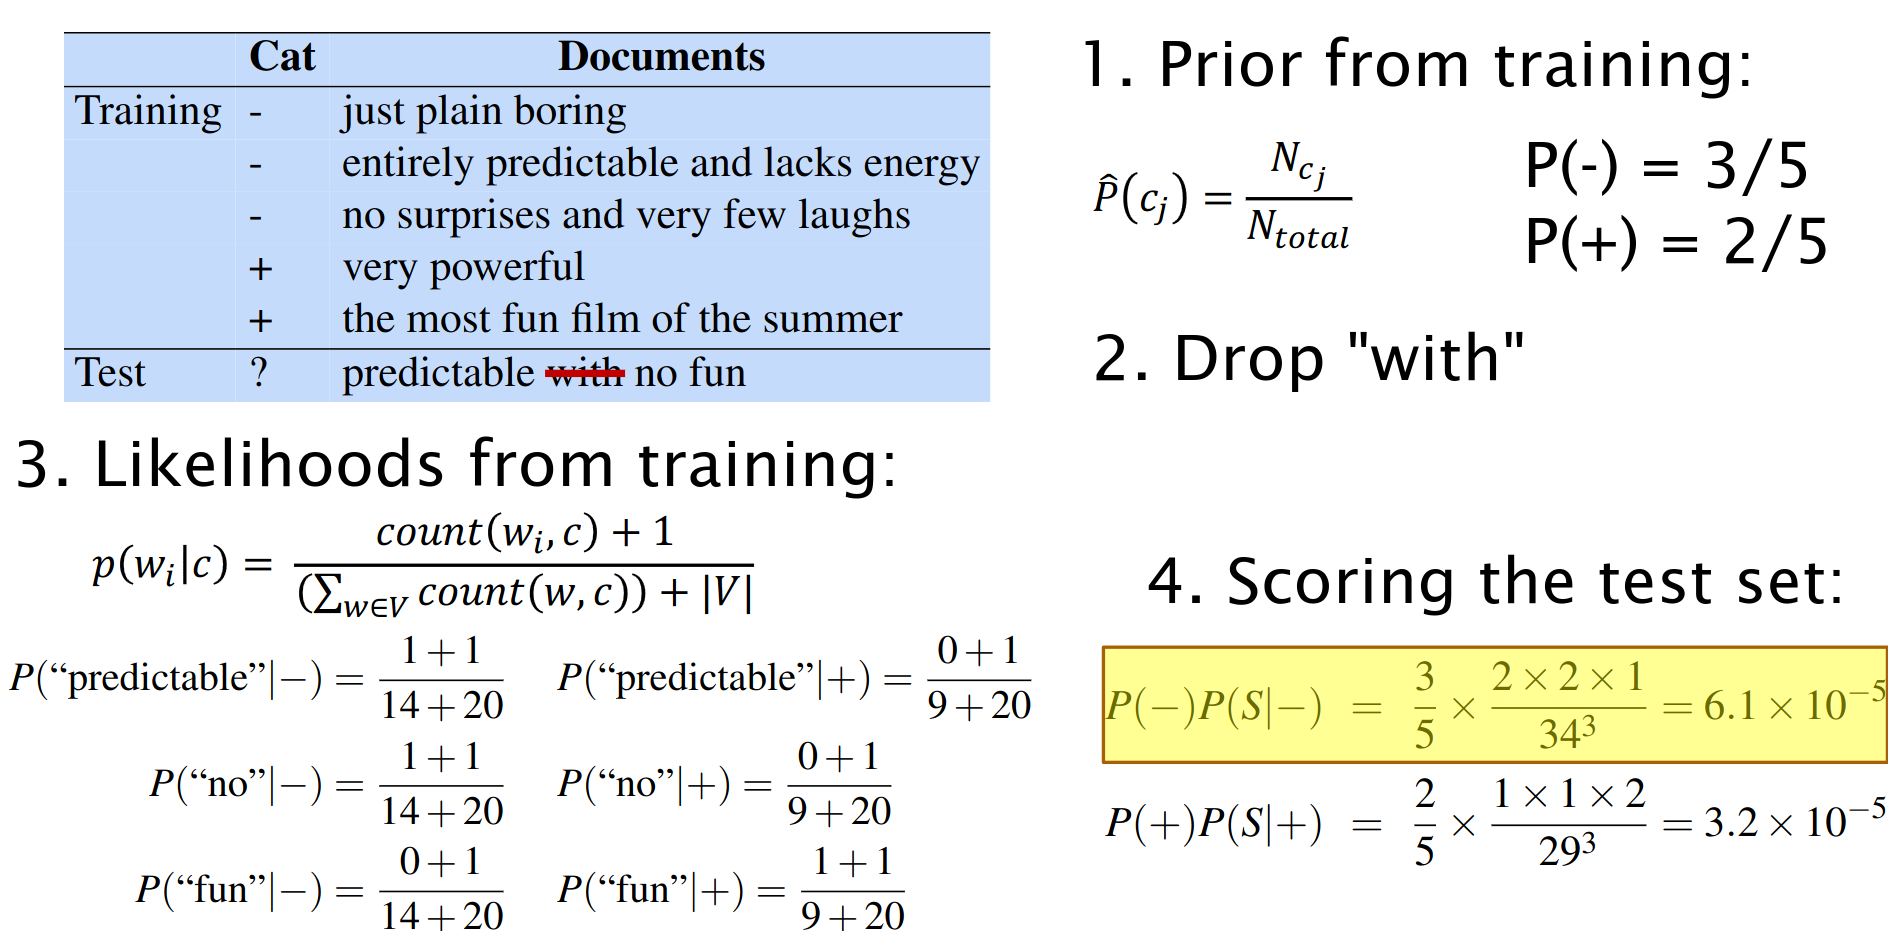
\includegraphics[scale = 0.23]{pics/naive_example.png}
\end{figure}

\section{Naive Bayes como modelo de lenguaje}

Cuando utilizamos características de palabras individuales y consideramos todas las palabras en el texto, el naive Bayes tiene una similitud importante con la modelización del lenguaje.

Específicamente, un modelo naive Bayes se puede ver como un conjunto de modelos de lenguaje de unigramas específicos de cada clase, en el que el modelo para cada clase instancia un modelo de lenguaje de unigrama.

Las características de verosimilitud del modelo naive Bayes asignan una probabilidad a cada palabra $P(\text{word}|c)$, y el modelo también asigna una probabilidad a cada oración:

\[P(s|c) = \prod_{i\in \text{positions}} P(w_i|c)\]

Consideremos un modelo naive Bayes con las clases positiva (+) y negativa (-) y los siguientes parámetros del modelo:

\begin{center}
\begin{tabular}{ccc}
\textbf{w} & $P(w|+)$ & $P(w|-)$ \\
I & 0.1 & 0.2 \\
love & 0.1 & 0.001 \\
this & 0.01 & 0.01 \\
fun & 0.05 & 0.005 \\
film & 0.1 & 0.1 \\
... & ... & ...
\end{tabular}
\end{center}

Cada una de las dos columnas anteriores instancian un modelo de lenguaje que puede asignar una probabilidad a la oración "I love this fun film":

\[P("\text{I love this fun film}"|+) = 0.1 \times 0.1 \times 0.01 \times 0.05 \times 0.1 = 0.0000005\]
\[P("\text{I love this fun film}"|-) = 0.2 \times 0.001 \times 0.01 \times 0.005 \times 0.1 = 0.0000000010\]

Como sucede, el modelo positivo asigna una probabilidad más alta a la oración:
\[P(s|\text{pos}) > P(s|\text{neg})\]

Cabe destacar que esto es solo la parte de verosimilitud del modelo naive Bayes; una vez que multiplicamos por la probabilidad a priori, un modelo naive Bayes completo podría tomar una decisión de clasificación diferente.



\section{Evaluación}

\begin{itemize}
 \item Consideremos solo tareas de clasificación de texto binario.
 \item Imagina que eres el CEO de Delicious Pie Company.
 \item Quieres saber lo que la gente está diciendo sobre tus pasteles.
 \item Por lo tanto, construyes un detector de tweets de "Delicious Pie" con las siguientes clases:
\begin{itemize}
\item Clase positiva: tweets sobre Delicious Pie Co.
\item Clase negativa: todos los demás tweets.
\end{itemize}
\end{itemize}



\subsection{La Matriz de Confusión 2x2}
\begin{table}[h]
\centering
\begin{tabular}{|c|c|c|}
\hline
\textbf{} & \textbf{Sistema Positivo} & \textbf{Sistema Negativo} \\
\hline
\textbf{Oro Positivo} & Verdadero Positivo (VP) & Falso Negativo (FN) \\
\hline
\textbf{Oro Negativo} & Falso Positivo (FP) & Verdadero Negativo (VN) \\
\hline
\end{tabular}
\end{table}

\textbf{Recall} (también conocido como \textbf{Sensibilidad} o \textbf{Tasa de Verdaderos Positivos}):
\[ \text{Recall} = \frac{VP}{VP + FN} \]

\textbf{Precisión}:
\[ \text{Precisión} = \frac{VP}{VP + FP} \]

\textbf{Exactitud}:
\[ \text{Exactitud} = \frac{VP + VN}{VP + FP + VN + FN} \]


\subsection{Evaluación: Exactitud}
¿Por qué no usamos la exactitud como nuestra métrica?

Imagina que vimos 1 millón de tweets:
\begin{itemize}
\item 100 de ellos hablaban sobre Delicious Pie Co.
\item 999,900 hablaban de otra cosa.
\end{itemize}

Podríamos construir un clasificador tonto que simplemente etiquete todos los tweets como "no sobre pasteles":
\begin{itemize}
\item ¡¡¡Obtendría una exactitud del 99.99\%!!! ¡¡¡Wow!!!
\item ¡Pero sería inútil! ¡No devuelve los comentarios que estamos buscando!
\end{itemize}

Por eso usamos precisión y recall en su lugar.

\subsection{Evaluación: Precisión y Recall}
\textbf{Precisión} mide el porcentaje de elementos que el sistema detectó (es decir, los elementos que el sistema etiquetó como positivos) que son realmente positivos (según las etiquetas de oro humanas).

\[
\text{Precisión} = \frac{\text{Verdaderos Positivos}}{\text{Verdaderos Positivos + Falsos Positivos}}
\]

\textbf{Recall} mide el porcentaje de elementos que el sistema identificó correctamente de todos los elementos que deberían haber sido identificados.

\[
\text{Recall} = \frac{\text{Verdaderos Positivos}}{\text{Verdaderos Positivos + Falsos Negativos}}
\]

\subsection{¿Por qué Precisión y Recall?}
Considera nuestro clasificador tonto de pasteles que simplemente etiqu

eta nada como "sobre pasteles".

\begin{itemize}
  \item Exactitud = 99.99\% (etiqueta correctamente la mayoría de los tweets como no relacionados con pasteles)
  \item Recall = 0 (no detecta ninguno de los 100 tweets relacionados con pasteles)
\end{itemize}

La precisión y el recall, a diferencia de la exactitud, enfatizan los verdaderos positivos:
\begin{itemize}
  \item Se centran en encontrar las cosas que se supone que debemos buscar.
\end{itemize}

\subsection{Una Medida Combinada: Medida F}
La medida F es un número único que combina la precisión (P) y el recall (R), definida como:
\[
F_\beta = \frac{(\beta^2+1)PR}{\beta^2P + R}
\]

La medida F, definida con el parámetro $\beta$, pondera diferencialmente la importancia del recall y la precisión.
\begin{itemize}
  \item $\beta > 1$ favorece al recall
  \item $\beta < 1$ favorece a la precisión
\end{itemize}

Cuando $\beta = 1$, la precisión y el recall son iguales, y tenemos la medida $F_1$ equilibrada:
\[
F_1 = \frac{2PR}{P + R}
\]

\subsection{Conjuntos de Prueba de Desarrollo ("Devsets")}

\begin{itemize}
 \item Para evitar el sobreajuste y proporcionar una estimación más conservadora del rendimiento, comúnmente utilizamos un enfoque de tres conjuntos: conjunto de entrenamiento, conjunto de desarrollo y conjunto de prueba.
\begin{figure}[h]
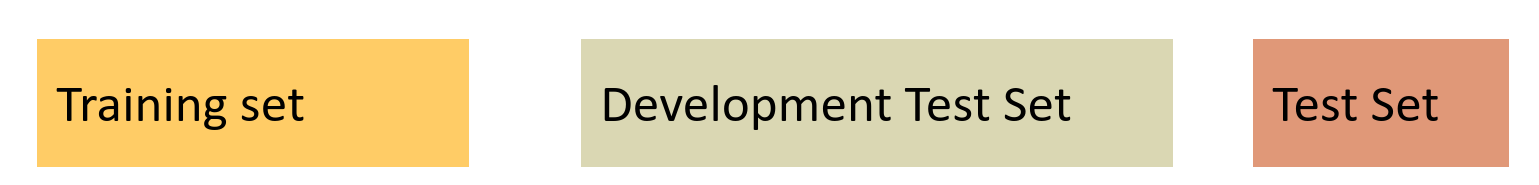
\includegraphics[scale = 0.23]{pics/devsets.png}
\end{figure}

\begin{itemize}
\item \textbf{Conjunto de entrenamiento}: Se utiliza para entrenar el modelo.
\item \textbf{Conjunto de desarrollo}: Se utiliza para ajustar el modelo y seleccionar los mejores hiperparámetros.
\item \textbf{Conjunto de prueba}: Se utiliza para informar el rendimiento final del modelo.
\end{itemize}

\item Este enfoque garantiza que el modelo no esté ajustado específicamente al conjunto de prueba, evitando el sobreajuste.
\item Sin embargo, crea una paradoja: queremos la mayor cantidad de datos posible para el entrenamiento, pero también para el conjunto de desarrollo.
\item ¿Cómo dividimos los datos?

\end{itemize}





\subsection{Validación Cruzada: Múltiples Divisiones}

\begin{itemize}
\item La validación cruzada nos permite utilizar todos nuestros datos para el entrenamiento y la prueba sin tener un conjunto de entrenamiento, conjunto de desarrollo y conjunto de prueba fijos.
\item Elegimos un número $k$ y dividimos nuestros datos en $k$ subconjuntos disjuntos llamados pliegues.
\item En cada iteración, uno de los pliegues se selecciona como conjunto de prueba mientras que los $k-1$ pliegues restantes se utilizan para entrenar el clasificador.
\item Calculamos la tasa de error en el conjunto de prueba y repetimos este proceso $k$ veces.
\item Finalmente, promediamos las tasas de error de estas $k$ ejecuciones para obtener una tasa de error promedio.
\item Por ejemplo, la validación cruzada de 10 pliegues implica entrenar 10 modelos con el 90\% de los datos y probar cada modelo por separado.
\item Las tasas de error resultantes se promedian para obtener la estimación final del rendimiento.
\item Sin embargo, la validación cruzada requiere que todo el corpus sea ciego, lo que impide examinar los datos para sugerir características o comprender el comportamiento del sistema.
\item Para abordar esto, se crea un conjunto de entrenamiento y un conjunto de prueba fijos, y se realiza la validación cruzada de 10 pliegues dentro del conjunto de entrenamiento.
\item La tasa de error se calcula convencionalmente en el conjunto de prueba.
\end{itemize}


\begin{center}
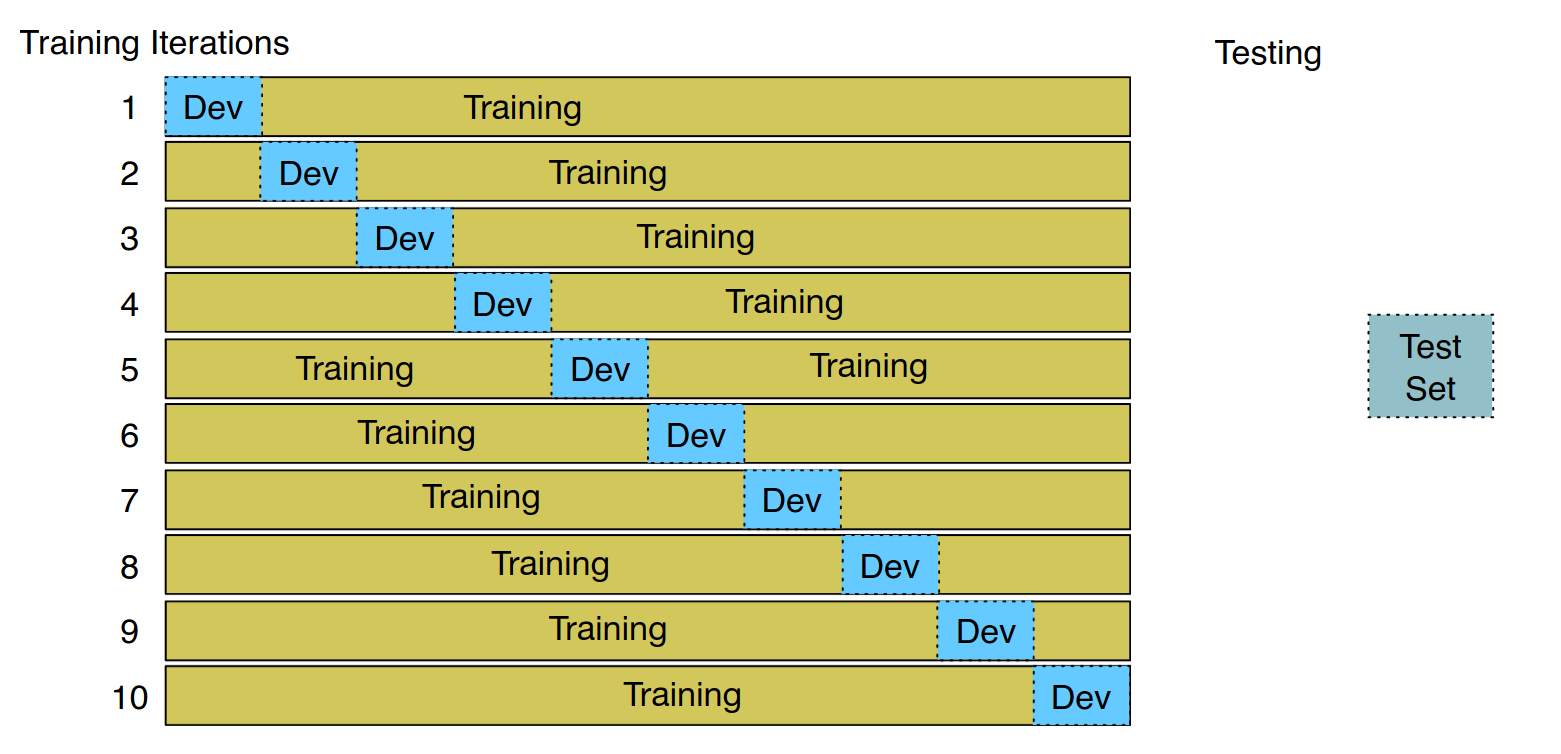
\includegraphics[scale=0.28]{pics/cv.png}
\end{center}


\subsection{Matriz de Confusión para clasificación de 3 clases}


\begin{center}
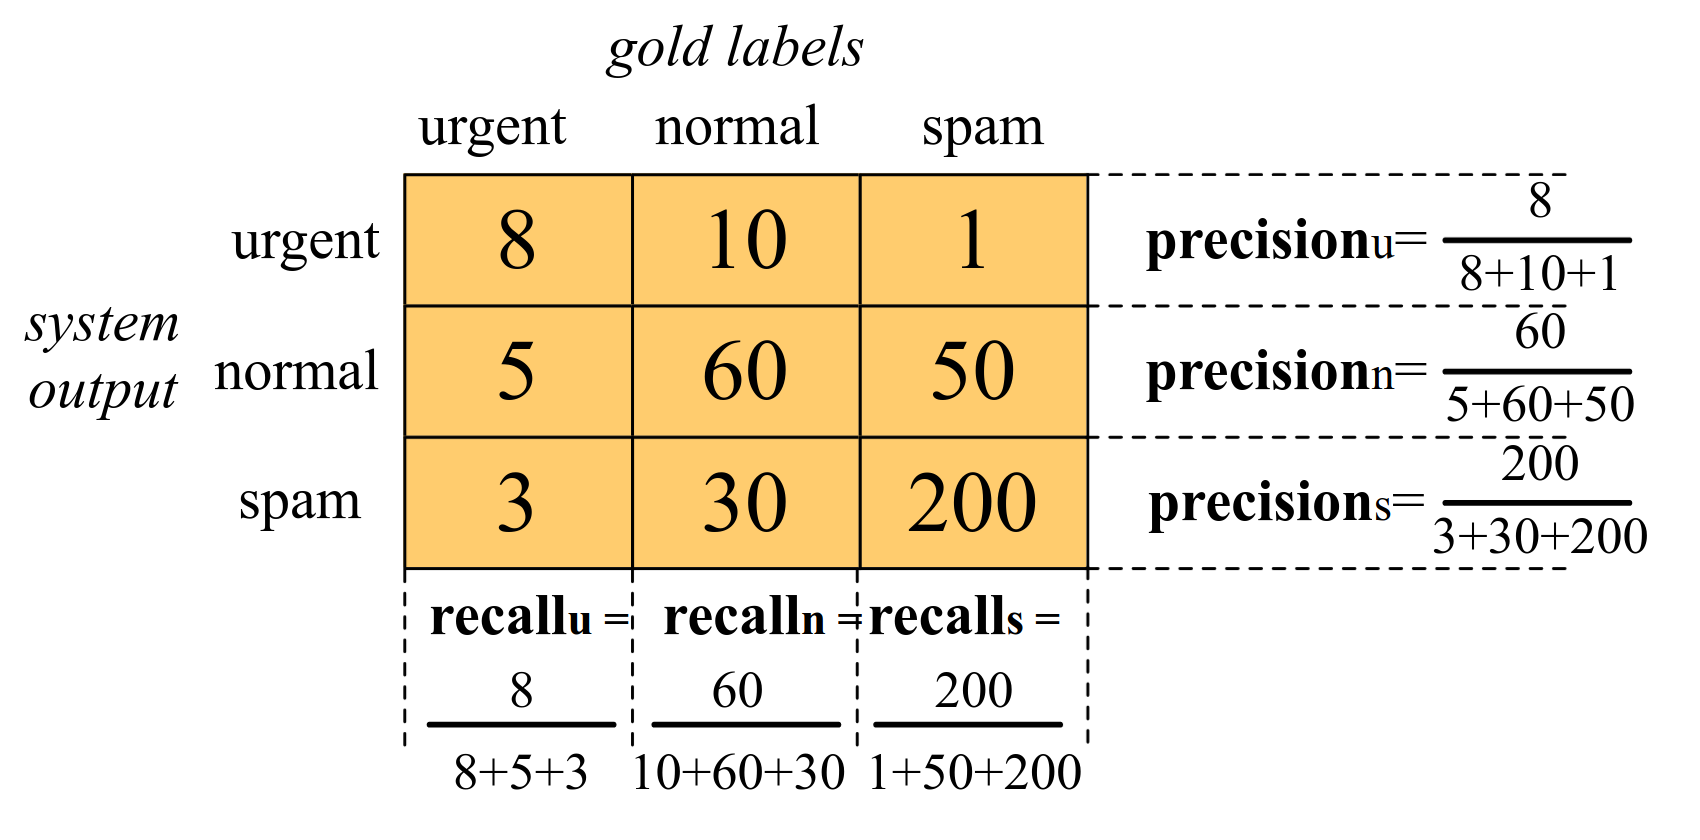
\includegraphics[scale=0.23]{pics/confmatrix.png}
\end{center}

Cómo combinar métricas binarias (Precisión, Recall, $F_1$) de más de 2 clases para obtener una métrica única:
\begin{itemize}
 \item Macro-promedio:
 \begin{itemize}
    \item Calcular las métricas de rendimiento (Precisión, Recall, $F_1$) para cada clase individualmente.
    \item Promediar las métricas en todas las clases.
 \end{itemize}
 \item Micro-promedio:
 \begin{itemize}
    \item Recopilar las decisiones para todas las clases en una matriz de confusión.
    \item Calcular la Precisión y el Recall a partir de la matriz de confusión.
 \end{itemize}
\end{itemize}

\begin{center}
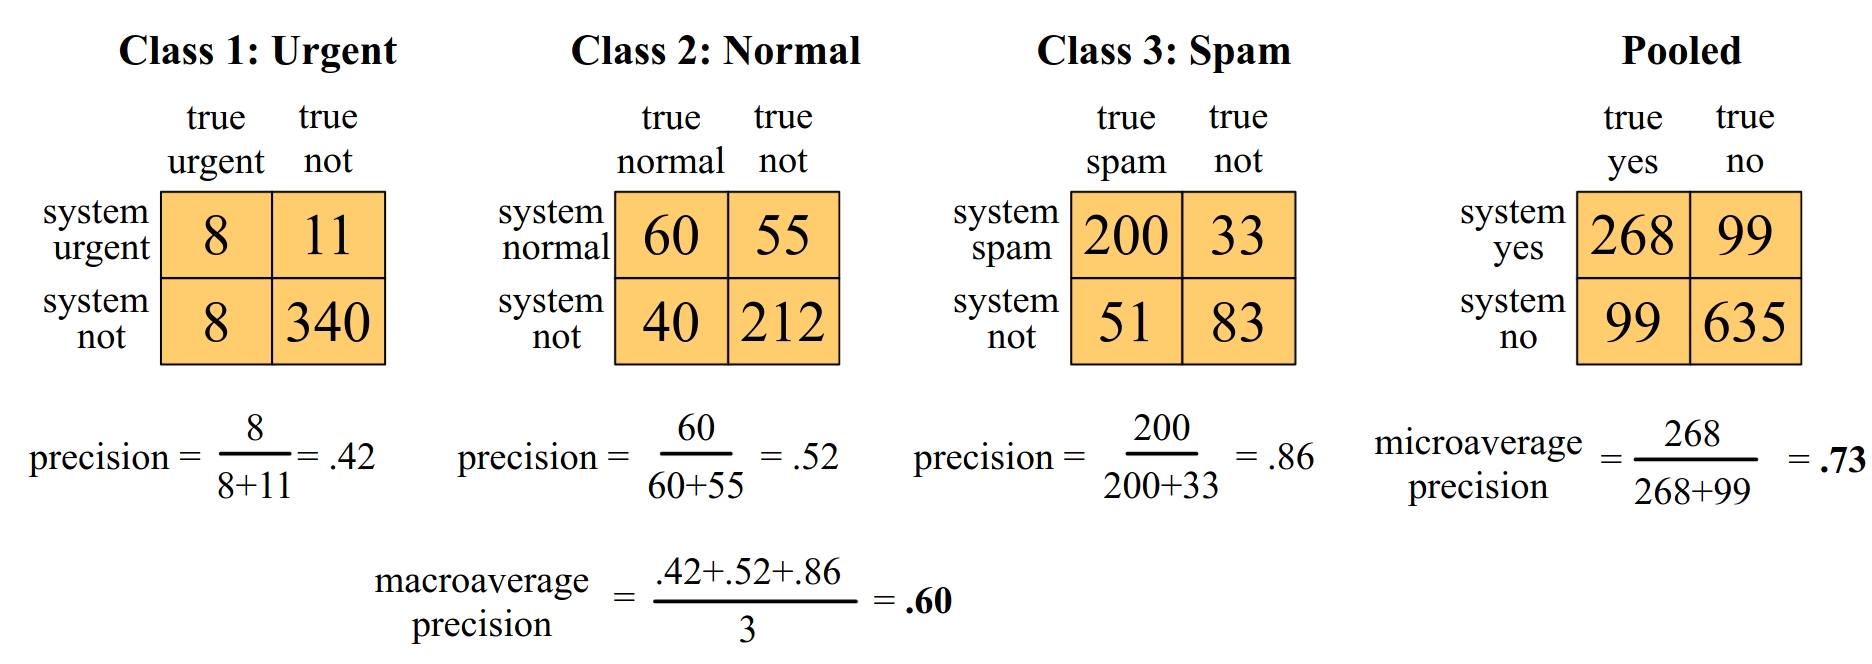
\includegraphics[scale=0.23]{pics/confmatrixmulti.png}
\end{center}



\chapter{Modelos Lineales}
\label{cap_lineales}

 Cuando hacemos aprendizaje supervisado, en escencia tenemos que buscar sobre el conjunto de todas las posibles funciones que pueden mapear desde las entradas hacia las salidas. Si no acotamos el espacio de busqueda de alguna forma nos encontramos con  un problema muy difícil (y bastante mal definido) \cite{goldberg2017neural}. A menudo nos limitamos a buscar dentro de familias específicas de funciones. Por ejemplo, el espacio de todas las funciones lineales con $d_{in}$ entradas y $d_{out}$ salidas. Estas familias de funciones se llaman clases de hipótesis. Al restringirnos a una clase de hipótesis específica, estamos inyectando al aprendiz con sesgo inductivo, es decir, un conjunto de suposiciones sobre la forma de la solución deseada. Algunas clases de hipótesis facilitan procedimientos eficientes para buscar la solución.

Una clase de hipótesis común es la de una función lineal de alta dimensión:

\begin{equation}
\begin{split}
f(\vec{x}) = \vec{x} \cdot W + \vec{b}\\
\vec{x} \in  \mathcal{R}^{d_{in}} & \quad W \in  \mathcal{R}^{d_{in}\times d_{out}} \quad \vec{b} \in  \mathcal{R}^{d_{out}}
\end{split}
\end{equation}

El vector $\vec{x}$ es la entrada de la función. La matriz $W$ y el vector $\vec{b}$ son los parámetros. El objetivo del aprendiz es establecer los valores de los parámetros $W$ y $\vec{b}$ de manera que la función se comporte como se pretende en una colección de valores de entrada $\vec{x}_{1:k} = \vec{x}_1,\dots,\vec{x}_k$ y las correspondientes salidas deseadas $\vec{y}_{1:k} = \vec{y}_1,\dots,\vec{y}_k$. La tarea de buscar en el espacio de funciones se reduce así a buscar en el espacio de parámetros.

\section{Ejemplo: Detección de Idiomas}

Consideremos la tarea de distinguir entre documentos escritos en inglés y documentos escritos en alemán. Este es un problema de clasificación binaria:

\begin{equation}
\begin{split}
f(\vec{x}) = \vec{x} \cdot \vec{w} + b
\end{split}
\end{equation}

donde $d_{out} = 1$, donde $\vec{w}$ es un vector y $b$ es un escalar. El rango de la función lineal es $[-\infty, \infty]$. Para usarla en la clasificación binaria, es común pasar la salida de $f(x)$ a través de la función $signo$, mapeando los valores negativos a -1 (clase negativa) y los valores no negativos a +1 (clase positiva).

Las frecuencias de letras son buenos predictores (características) para esta tarea, pero aún más informativos son los recuentos de bigramas de letras, es decir, pares de letras consecutivas. Es probable que nos encontremos con un documento nuevo sin ninguna de las palabras que observamos en el conjunto de entrenamiento, mientras que un documento sin ninguno de los distintivos bigramas de letras es significativamente menos probable \cite{goldberg2017neural}. Supongamos que tenemos un alfabeto de 28 letras (a-z, espacio y un símbolo especial para todos los demás caracteres, incluidos dígitos, puntuación, etc.). Los documentos se representan como vectores de dimensión $28 \times 28$, es decir, $\vec{x} \in \mathcal{R}^{784}$. Cada entrada $\vec{x}_{[i]}$ representa un recuento de una combinación particular de letras en el documento, normalizado por la longitud del documento. Por ejemplo, si denotamos por $\vec{x}_{ab}$ la entrada de $\vec{x}$ correspondiente al bigrama de letras $ab$:

\begin{equation}
\vec{x}_{ab} = \frac{\#ab}{|D|}
\end{equation}

donde $\#ab$ es el número de veces que aparece el bigrama $ab$ en el documento y $|D|$ es el número total de bigramas en el documento (la longitud del documento).

La figura muestra histogramas de bigramas de caracteres para documentos en inglés y alemán. Los guiones bajos representan espacios. Solo se muestran los bigramas de caracteres más frecuentes.

\begin{figure}[htb]
	\centering
	 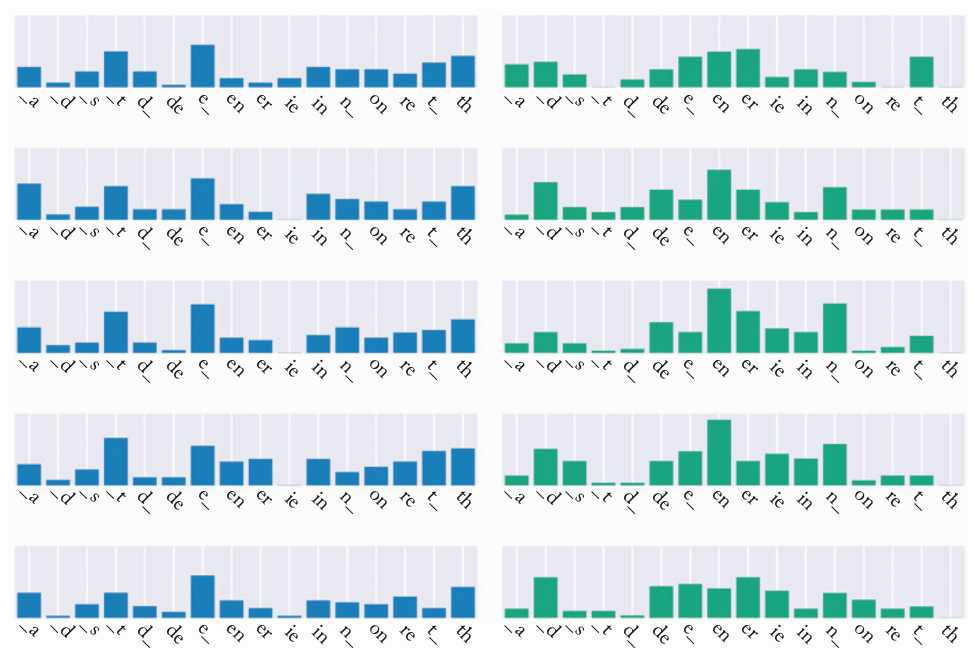
\includegraphics[scale=0.26]{pics/langbigrams.png}
\end{figure}

Fuente: \cite{goldberg2017neural}

La figura anterior muestra patrones claros en los datos. Dado un nuevo elemento, por ejemplo:

\begin{figure}[htb]
	\centering
	 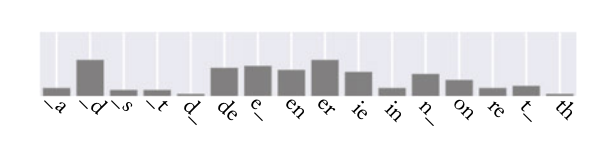
\includegraphics[scale=0.4]{pics/langbigramstest.png}
\end{figure}

Probablemente podríamos decir que es más similar al grupo alemán que al grupo inglés (observar la frecuencia de "th" y "ie"). No podemos usar una regla única definitiva como "si tiene th es inglés" o "si tiene ie es alemán". Aunque los textos en alemán tienen considerablemente menos "th" que el inglés, la combinación "th" puede ocurrir en textos en alemán, al igual que la combinación "ie" puede ocurrir en inglés. La decisión requiere ponderar diferentes factores relativos entre sí.

Podemos formalizar el problema en un entorno de aprendizaje automático utilizando un modelo lineal:

\begin{equation}
\begin{split}
\hat{y} = \text{sign}(\vec{x}\cdot \vec{w} + b) = \text{sign}(\vec{x}_{aa}\times \vec{w}_{aa}+ \vec{x}_{ab}\times \vec{w}_{ab}+ \vec{x}_{ac}\times \vec{w}_{ac} \dots +b)
\end{split}
\end{equation}

Un documento se considerará inglés si $f(\vec{x}) \geq 0$ y alemán en caso contrario. La intuición detrás del aprendizaje es la siguiente:

\begin{enumerate}
\item El aprendizaje debe asignar valores positivos grandes a las entradas de $\vec{w}$ asociadas con pares de letras que son mucho más comunes en inglés que en alemán (por ejemplo, "th").
\item También debe asignar valores negativos a los pares de letras que son mucho más comunes en alemán que en inglés (por ejemplo, "ie", "en").
\item Finalmente, debe asignar valores alrededor de cero a los pares de letras que son comunes o raros en ambos idiomas.
\end{enumerate}


%Translate this Latex book chapter to Spanish. Output in Latex format. Rearrange bullet points (\items) into full paragraphs. Make sure that sentences are connected in a more fluid way as they come.
\section{Clasificación binaria log-lineal}
La salida $f(\vec{x})$ se encuentra en el rango $[-\infty,\infty]$, y la mapeamos a una de las dos clases $\{-1,+1\}$ utilizando la función $signo$. Esto es adecuado si lo único que nos importa es la clase asignada. Sin embargo, puede que también estemos interesados en la confianza de la decisión o en la probabilidad que el clasificador asigna a la clase.

Una alternativa que facilita esto es mapear la salida al rango $[0,1]$ mediante una función de compresión como la función sigmoide $\sigma(x)$:

\begin{equation}
\sigma(x) = \frac{1}{1+e^{-x}}
\end{equation}

lo que resulta en:

\begin{equation}
\hat{y}=\sigma(f(\vec{x})) = \frac{1}{1+e^{-\vec{x}\cdot \vec{w}+b}}
\end{equation}

La función sigmoide es monótona creciente y mapea los valores al rango $[0, 1]$, con $0$ mapeado a $\frac{1}{2}$. Cuando se utiliza con una función de pérdida adecuada (que se discutirá más adelante), las predicciones binarias realizadas mediante el modelo log-lineal se pueden interpretar como estimaciones de la probabilidad de pertenencia a la clase:

\begin{equation}
 \sigma(f(\vec{x})) = P(\hat{y} = 1| \vec{x}) \quad \text{de que $\vec{x}$ pertenezca a la clase positiva.}
\end{equation}

También obtenemos $P(\hat{y} = 0| \vec{x}) = 1 - P(\hat{y} = 1| \vec{x}) = 1-\sigma(f(\vec{x}))$. Cuanto más cercano sea el valor a $0$ o $1$, más seguro está el modelo en su predicción de pertenencia a la clase, y el valor $0.5$ indica incertidumbre del modelo.

\section{Clasificación multiclase}
La mayoría de los problemas de clasificación son de naturaleza multiclase: se asignan ejemplos a una de las $k$ clases diferentes. Por ejemplo, se nos puede dar un documento y se nos pide clasificarlo en uno de los seis posibles idiomas: inglés, francés, alemán, italiano, español y otros.

Una solución posible es considerar seis vectores de pesos $\vec{w}_{EN}$, $\vec{w}_{FR}$, $\dots$ y sesgos (uno para cada idioma). Predecimos el idioma que resulta en el puntaje más alto:

\begin{equation}
 \hat{y} = f(\vec{x}) = \operatorname{argmax}_{L \in \{ EN,FR,GR,IT,SP,O \}} \quad \vec{x}\cdot \vec{w}_L+ b_{L}
\end{equation}

Los seis conjuntos de parámetros $\vec{w}_L \in  \mathcal{R}^{784}$ y $b_L$ se pueden organizar en una matriz $W \in \mathcal{R}^{784\times6}$ y un vector $\vec{b} \in \mathcal R^6$, y la ecuación se puede reescribir como:

\begin{equation}
 \begin{split}
  \vec{\hat{y}} = f(\vec{x}) = \quad & \vec{x} \cdot W + \vec{b}\\
   \text{predicción} = \hat{y} = \quad  & \operatorname{argmax}_i \vec{\hat{y}}_{[i]}
 \end{split}
\end{equation}

Aquí, $\vec{\hat{y}} \in \mathcal{R}^6$ es un vector de los puntajes asignados por el modelo a cada idioma, y determinamos el idioma predicho tomando el argmax sobre las entradas de $\vec{\hat{y}}$ (las columnas con el valor más alto).

\section{Representaciones}
Consideremos el vector $\vec{\hat{y}}$ resultante de aplicar un modelo entrenado a un documento. Podemos considerar que este vector es una representación del documento, ya que captura las propiedades del documento que son importantes para nosotros, es decir, los puntajes de los diferentes idiomas. La representación $\vec{\hat{y}}$ contiene estrictamente más información que la predicción $\operatorname{argmax}_i \vec{\hat{y}}_{[i]}$.

Por ejemplo, $\vec{\hat{y}}$ se puede utilizar para distinguir documentos en los que el idioma principal es el alemán, pero que también contienen una cantidad considerable de palabras en francés. El agrupamiento de documentos basado en $\vec{\hat{y}}$ podría ayudar a descubrir documentos escritos en dialectos regionales o por autores multilingües.

Los vectores $\vec{x}$ que contienen los recuentos normalizados de los bigramas de letras para los documentos también son representaciones de los documentos. Se podría argumentar que contienen un tipo de información similar a los vectores $\vec{\hat{y}}$. Sin embargo, las representaciones en $\vec{\hat{y}}$ son más compactas (6 entradas en lugar de 784) y más especializadas para el objetivo de predicción de idioma. El agrupamiento por los vectores $\vec{x}$ probablemente revelaría similitudes en los documentos que no se deben a una mezcla particular de idiomas, sino tal vez al tema o estilo de escritura del documento.

La matriz entrenada $W \in \mathcal{R}^{784 \times 6}$ también se puede considerar como una representación aprendida. Podemos considerar dos vistas de $W$, como filas o como columnas.

\begin{figure}[htb]
	\centering
	 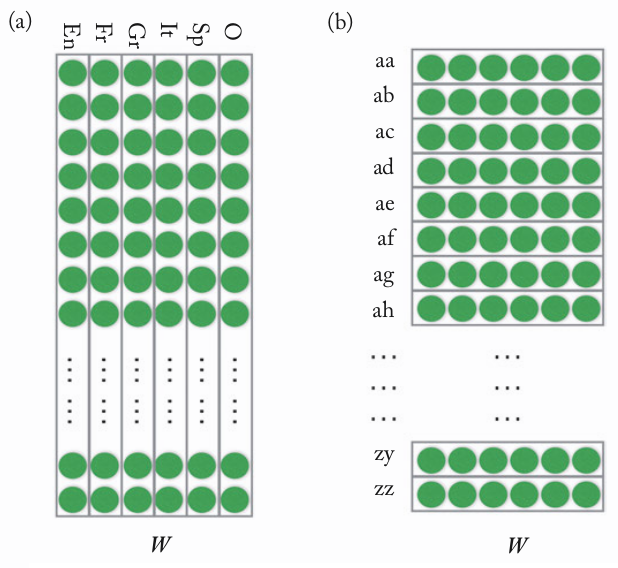
\includegraphics[scale=0.35]{pics/2rep.png}
\end{figure}

Dos vistas de la matriz $W$. (a) Cada columna corresponde a un idioma. (b) Cada fila corresponde a un bigrama de letras. Fuente: \cite{goldberg2017neural}.

Una columna de $W$ puede tomarse como una representación vectorial de $784$ dimensiones de un idioma en términos de sus patrones característicos de bigramas de letras. Luego, podemos agrupar los 6 vectores de idioma según su similitud. Cada una de las 784 filas de $W$ proporciona una representación vectorial de 6 dimensiones de ese bigrama en términos de los idiomas que promueve. Las representaciones son fundamentales para el aprendizaje profundo. Se podría argumentar que el principal poder del aprendizaje profundo es la capacidad de aprender buenas representaciones.

En el caso lineal, las representaciones son interpretables, ya que podemos asignar una interpretación significativa a cada dimensión en el vector de representación. Por ejemplo, cada dimensión puede corresponder a un idioma o a un determinado bigrama de letras.

Por otro lado, los modelos de aprendizaje profundo a menudo aprenden una cascada de representaciones de la entrada que se construyen una encima de la otra. Estas representaciones a menudo no son interpretables, es decir, no sabemos qué propiedades de la entrada capturan. Sin embargo, siguen siendo muy útiles para hacer predicciones.

\section{Representación de Vectores One-Hot}
El vector de entrada $\vec{x}$ en nuestro ejemplo de clasificación de idioma contiene los recuentos normalizados de los bigramas en el documento $D$. Este vector se puede descomponer en un promedio de $|D|$ vectores, cada uno correspondiente a una posición particular del documento $i$:

\begin{equation}
 \vec{x} = \frac{1}{|D|} \sum_{i=1}^{|D|} \vec{x}^{D_{[i]}}
\end{equation}

Aquí, $D_{[i]}$ es el bigrama en la posición $i$ del documento. Cada vector $\vec{x}^{D_{[i]}} \in \mathcal{R}^{784}$ es un vector one-hot, lo que significa que todos los elementos son cero excepto la única entrada que corresponde al bigrama de letras $D_{[i]}$, que es 1. El vector resultante $\vec{x}$ se conoce comúnmente como un promedio de bolsa de bigramas (más generalmente, una bolsa de palabras promediada, o simplemente una bolsa de palabras).

Las representaciones de bolsa de palabras contienen información sobre las identidades de todas las "palabras" (en este caso, bigramas) del documento, sin considerar su orden. Una representación one-hot se puede considerar como una bolsa de una sola "palabra".

\begin{figure}[htb]
	\centering
	 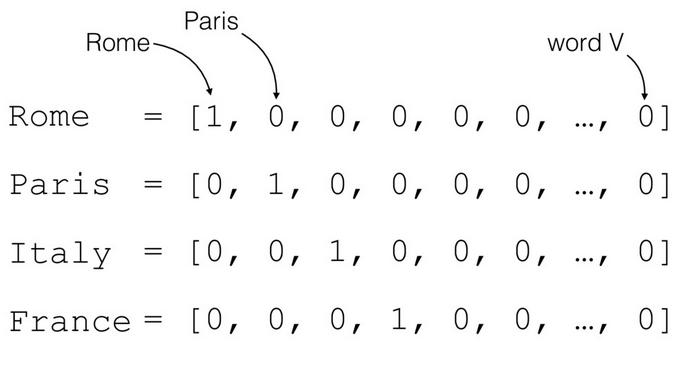
\includegraphics[scale=0.3]{pics/onehot.png}
\end{figure}

Vectores one-hot de palabras.

Fuente: \url{https://medium.com/@athif.shaffy/one-hot-encoding-of-text-b69124bef0a7}.

%Translate this Latex book chapter to Spanish. Output in Latex format. Rearrange bullet points (\items) into full paragraphs. Make sure that sentences are connected in a more fluid way as they come.\section{Clasificación Log-lineal de Múltiples Clases}
En el caso binario, transformamos la predicción lineal en una estimación de probabilidad al pasarla por la función sigmoide, lo que resulta en un modelo log-lineal. En el caso de múltiples clases, el análogo es pasar el vector de puntajes a través de la función \textbf{softmax}:

\begin{equation}
 \operatorname{softmax}(\vec{x})_{[i]} = \frac{e^{\vec{x}_{[i]}}}{\sum_j e^{\vec{x}_{[j]}}}
\end{equation}

Lo que resulta en:

\begin{equation}
\begin{split}
\vec{\hat{y}} \quad & =  \operatorname{softmax}(\vec{x} \cdot W + \vec{b})  \\
\vec{\hat{y}}_{[i]} \quad & = \frac{e^{(\vec{x} \cdot W + \vec{b})_{[i]}}}{\sum_j e^{(\vec{x} \cdot W + \vec{b})_{[j]}}}
\end{split}
\end{equation}

La transformación softmax fuerza a los valores en $\hat{\vec{y}}$ a ser positivos y sumar 1, lo que los hace interpretables como una distribución de probabilidad.

\section{Entrenamiento}
Cuando se entrena una función parametrizada (por ejemplo, un modelo lineal, una red neuronal), se define una función de pérdida $L(\hat{y}, y)$, que establece la pérdida al predecir $\hat{y}$ cuando la salida verdadera es $y$.

\begin{displaymath}
L(f(\vec{x};\Theta), y)
\end{displaymath}

Utilizamos el símbolo $\Theta$ para denotar todos los parámetros del modelo (por ejemplo, $W, \vec{b}$).

El objetivo del entrenamiento es minimizar la pérdida en los diferentes ejemplos de entrenamiento. Formalmente, una función de pérdida $L(\hat{y},y)$ asigna una puntuación numérica (un escalar) a una salida predicha $\hat{y}$ dada la salida esperada verdadera $y$. La función de pérdida debería alcanzar su valor mínimo para los casos en los que la predicción sea correcta.

También podemos definir una pérdida en todo el corpus con respecto a los parámetros $\Theta$ como la pérdida promedio en todos los ejemplos de entrenamiento:

\begin{displaymath}
 \mathcal{L}(\Theta) = \frac{1}{n} \sum_{i=1}^n L(f(\vec{x}_i;\Theta), y_i)
\end{displaymath}

El objetivo del algoritmo de entrenamiento es establecer los valores de los parámetros $\Theta$ de manera que el valor de $\mathcal{L}$ se minimice.

\begin{displaymath}
 \hat{\Theta} = \operatorname{argmin}_{\Theta} \mathcal{L}(\Theta) =  \operatorname{argmin}_{\Theta} \frac{1}{n} \sum_{i=1}^n L(f(\vec{x}_i;\Theta), y_i)
\end{displaymath}

\subsection{Optimización basada en Gradiente}
Las funciones se

entrenan utilizando métodos basados en gradientes. Estos métodos funcionan mediante el cálculo repetido de una estimación de la pérdida $L$ sobre el conjunto de entrenamiento. El método de entrenamiento calcula los gradientes de los parámetros ($\Theta$) con respecto a la estimación de pérdida y mueve los parámetros en la dirección opuesta al gradiente. Los diferentes métodos de optimización difieren en cómo se calcula la estimación de error y cómo se define el movimiento en la dirección opuesta al gradiente.

Si la función es convexa, el óptimo será global. De lo contrario, el proceso solo garantiza encontrar un óptimo local.

\begin{figure}[htb]
	\centering
	 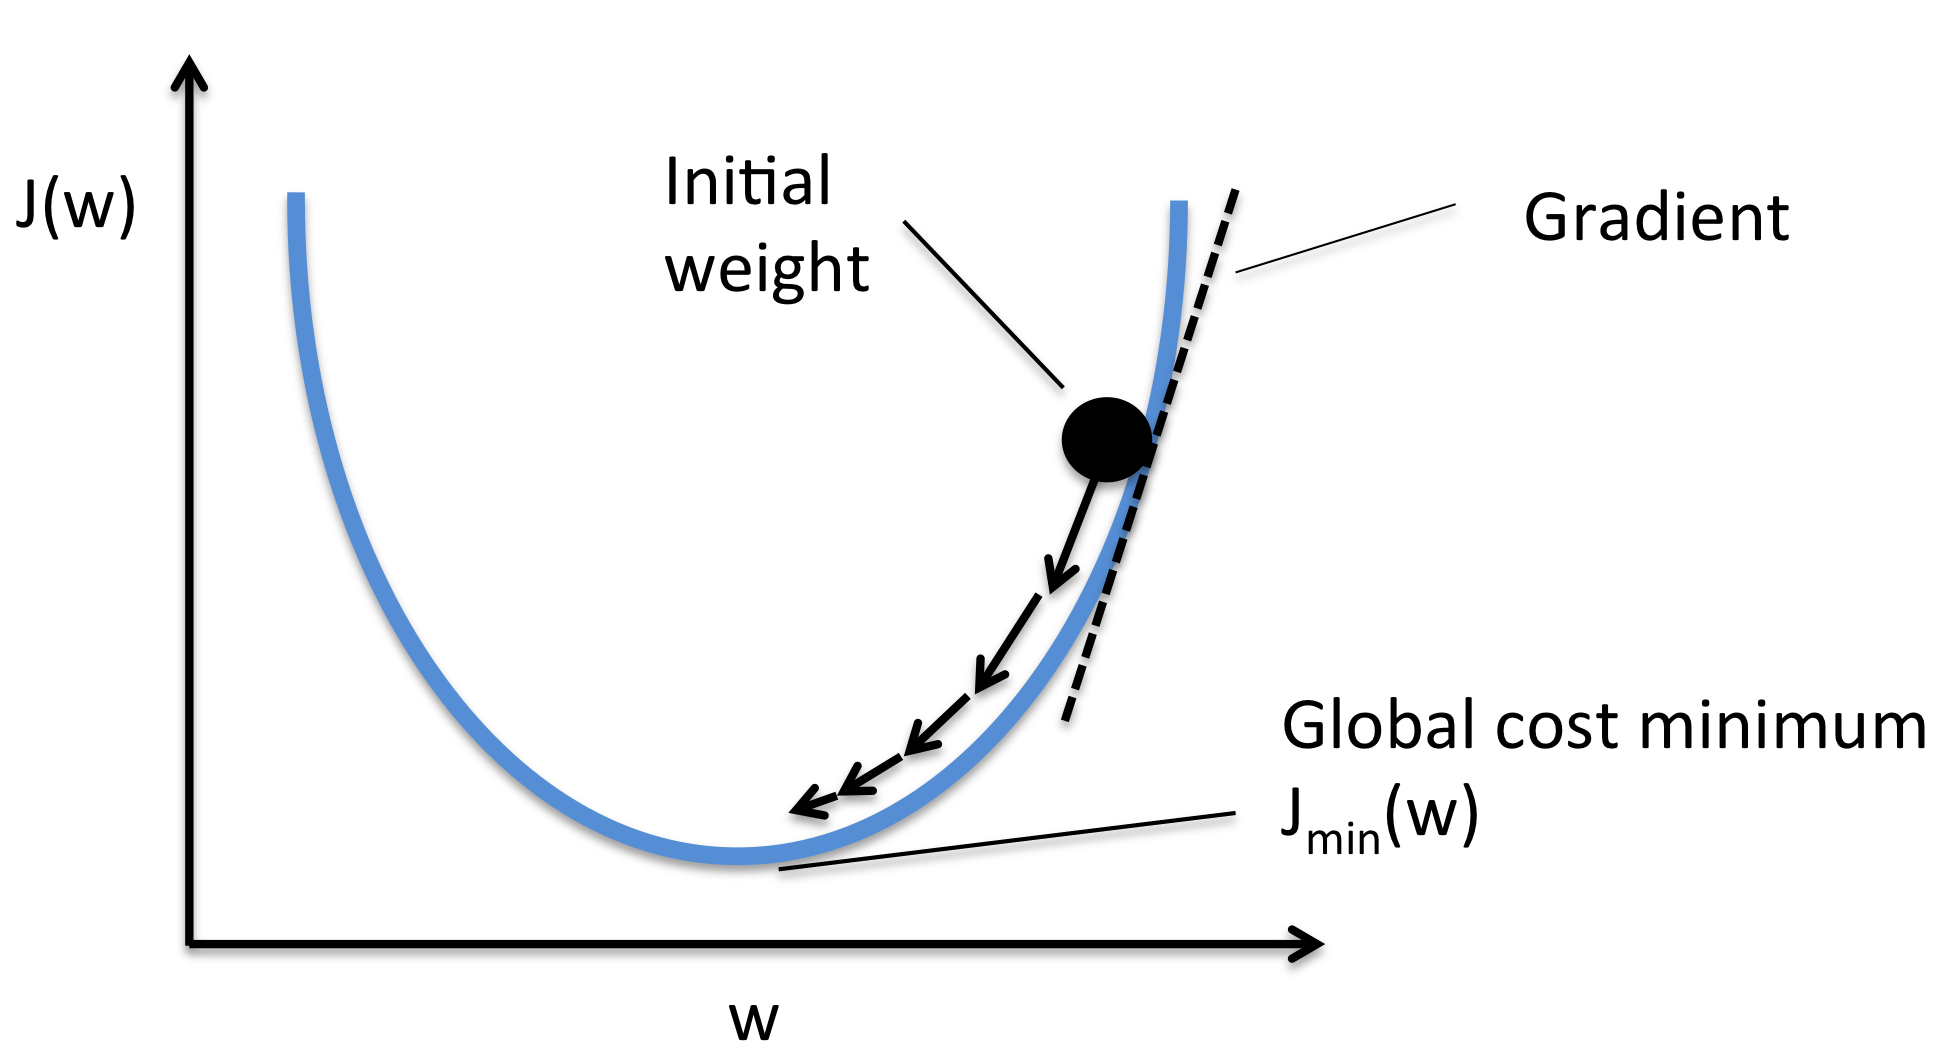
\includegraphics[scale=0.15]{pics/sgd.png}
\end{figure}
\footnotetext{Fuente: \url{https://sebastianraschka.com/images/faq/closed-form-vs-gd/ball.png}}

\begin{figure}[htb]
	\centering
	 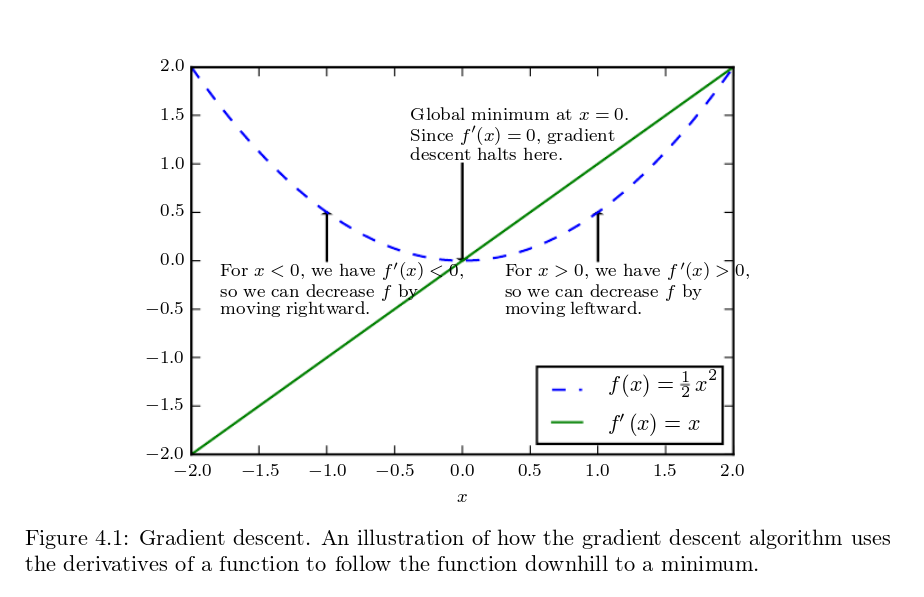
\includegraphics[scale=0.45]{pics/gradientdescent.png}
\end{figure}
\footnotetext{\cite{goodfellow2016deep}}

\subsection{Descenso de Gradiente Estocástico en Línea}
\begin{itemize}
\item Todos los parámetros se inicializan con valores aleatorios ($\Theta$).
\item Para cada ejemplo de entrenamiento $(x,y)$, calculamos la pérdida $L$ con los valores actuales de $\Theta$.
\item Luego actualizamos los parámetros con la siguiente regla hasta que se alcance la convergencia:
\item $\Theta_i \leftarrow \Theta_i - \eta \frac{\partial L}{\Theta_i}(\hat{y},y)$ (para todos los parámetros $\Theta_i$)
\end{itemize}

\begin{figure}[htb]
	\centering
	 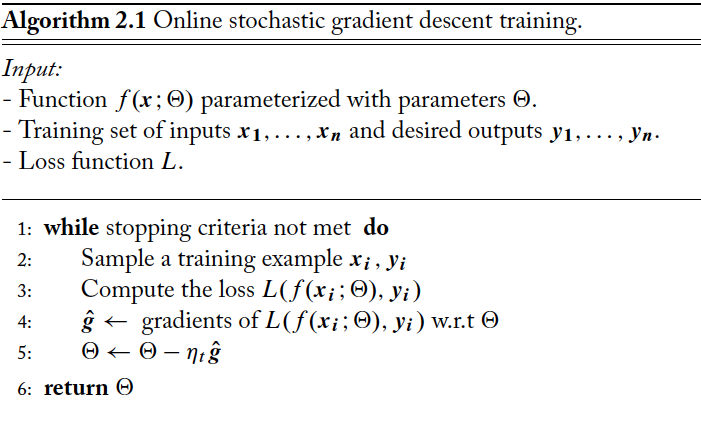
\includegraphics[scale=0.3]{pics/Online-SGD.png}
\end{figure}
\footnotetext{Fuente:\cite{goldberg2017neural}}

La tasa de aprendizaje puede ser fija durante todo el proceso de entrenamiento o puede decrecer como función del paso de tiempo $t$. El error calculado en la línea 3 se basa en un solo ejemplo de entrenamiento y, por lo tanto, es solo una estimación aproximada de la pérdida en todo el corpus $L$ que queremos minimizar. El ruido en el cálculo de la pérdida puede resultar en gradientes inexactos (los ejemplos individuales pueden proporcionar información ruidosa).

\subsection{Descenso de Gradiente Estocástico en Mini-batch}
\begin{itemize}
\item Una forma común de reducir este ruido es estimar el error y los gradientes en función de una muestra de $m$ ejemplos.
\item Esto da lugar al algoritmo de SGD en mini-batch.
\end{itemize}

\begin{figure}[htb]
	\centering
	 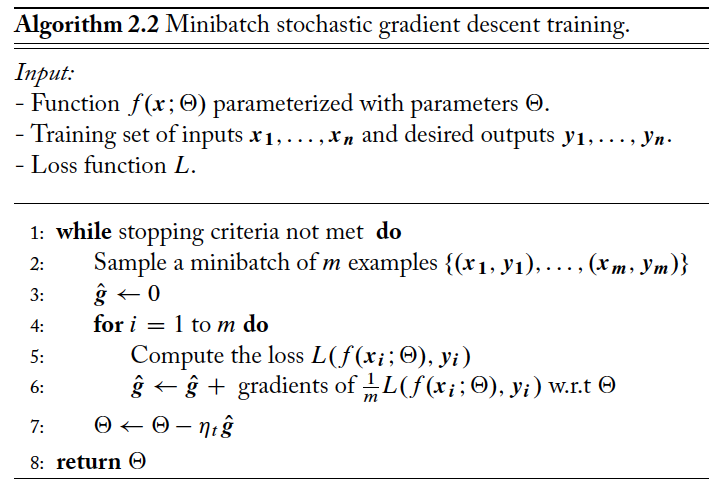
\includegraphics[scale=0.25]{pics/minibatch-SGD.png}
\end{figure}

Valores más altos de $m$ proporcionan mejores estimaciones de los gradientes en todo el corpus, mientras que valores más pequeños permiten más actualizaciones y, a su vez, una convergencia más rápida.

Para tamaños moderados de

$m$, algunas arquitecturas de cómputo (por ejemplo, GPUs) permiten una implementación paralela eficiente del cálculo en las líneas 3-6.

\footnotetext{Fuente:\cite{goldberg2017neural}}


%Translate this Latex book chapter to Spanish. Output in Latex format. Rearrange bullet points (\items) into full paragraphs. Make sure that sentences are connected in a more fluid way as they come.
\subsection{Funciones de Pérdida}
Las funciones de pérdida son utilizadas en algoritmos de aprendizaje automático para medir la discrepancia entre las predicciones del modelo y los valores reales de los datos de entrenamiento. Algunas funciones de pérdida comunes son:

\begin{itemize}
 \item Pérdida Hinge (o pérdida SVM): utilizada en problemas de clasificación binaria, donde la salida del clasificador es un escalar $\tilde{y}$ y la salida deseada $y$ está en el conjunto $\{+1,-1\}$. La regla de clasificación es $\hat{y} = \text{signo}(\tilde{y})$, y se considera una clasificación correcta si $y \cdot \tilde{y} > 0$. La función de pérdida se define como:
 \begin{displaymath}
  L_{\text{hinge(binaria)}}(\tilde{y},y) = \max(0,1-y \cdot \tilde{y})
 \end{displaymath}

 \item Entropía cruzada binaria (o pérdida logística): utilizada en clasificación binaria con salidas de probabilidad condicional. La salida del clasificador $\tilde{y}$ se transforma utilizando la función sigmoide para que esté en el rango $[0,1]$, y se interpreta como la probabilidad condicional $P(y=1|x)$. La función de pérdida se define como:
  \begin{displaymath}
  L_{\text{logística}}(\hat{y},y) = -y \log \hat{y} - (1-y) \log(1-\hat{y})
 \end{displaymath}

 \item La pérdida logística tiene una interpretación probabilística. Se asume que $P(y =1 | \vec{x} ; \Theta) = \sigma(f(\vec{x})) = \frac{1}{1+e^{-\vec{x}\cdot \vec{w}+b}}$ y $P(y = 0 | \vec{x} ; \Theta) = 1 - \sigma(f(\vec{x}))$. Esto se puede escribir de manera más compacta como:
 \begin{displaymath}
  P(y | \vec{x} ; \Theta) = \sigma(f(\vec{x}))^y\times(1-\sigma(f(\vec{x})))^{1-y}
 \end{displaymath}

 \item La expresión anterior es la función de masa de probabilidad de la distribución de Bernoulli.

 \item Si reemplazamos $\sigma(f(\vec{x}))$ por $\hat{y}$, obtenemos:
 \begin{displaymath}
  P(y | \vec{x} ; \Theta) = \hat{y}^y\times(1-\hat{y})^{1-y}
 \end{displaymath}
 \item Si aplicamos la estimación de máxima verosimilitud a esta expresión y tomamos el logaritmo, obtenemos:
 \begin{displaymath}
  y \log \hat{y} + (1-y) \log(1-\hat{y})
 \end{displaymath}

 \item ¡Maximizar esta expresión es equivalente a minimizar la pérdida logística!

 \item ¡Muchas funciones de pérdida corresponden al logaritmo negativo de la verosimilitud de modelos probabilísticos!



\item Pérdida de entropía cruzada categórica: se utiliza cuando se desea una interpretación probabilística de las puntuaciones de múltiples clases. Mide la discrepancia entre la distribución de etiquetas reales $\vec{y}$ y la distribución de etiquetas predichas $\vec{\hat{y}}$. La función de pérdida se define como:
\begin{displaymath}
L_{\text{entropía cruzada}}(\vec{\hat{y}},\vec{y}) = - \sum_{i} \vec{y}_{[i]} \log(\vec{\hat{y}}_{[i]})
\end{displaymath}

\item Cuando se utiliza la pérdida de entropía cruzada, se asume que la salida del clasificador se transforma utilizando la función softmax.

\item La función softmax comprime la salida de $k$ dimensiones a valores en el rango (0,1) de modo que todas las entradas sumen 1. Por lo tanto, $\vec{\hat{y}}_{[i]} = P(y = i |x)$ representa la distribución de pertenencia a la clase condicional.

\item Para problemas de clasificación dura en los que cada ejemplo de entrenamiento tiene una única asignación de clase correcta, $\vec{y}$ es un vector one-hot que representa la clase verdadera. En tales casos, la entropía cruzada se simplifica a:
\begin{displaymath}
L_{\text{entropía cruzada (clasificación dura)}}(\vec{\hat{y}},\vec{y}) = -\log(\vec{\hat{y}}_{[t]})
\end{displaymath}
donde $t$ es la asignación de clase correcta.

\end{itemize}

\section{Regularización}
Nuestro problema de optimización puede tener múltiples soluciones y, especialmente en dimensiones más altas, puede sufrir de sobreajuste. Consideremos el siguiente escenario en nuestro problema de identificación de idioma: uno de los documentos en el conjunto de entrenamiento ($\vec{x}_O$) es un valor atípico. En realidad, el documento está en alemán, pero está etiquetado como francés.

Para reducir la pérdida, el modelo puede identificar características (bigramas de letras) en $\vec{x}_O$ que ocurren en pocos otros documentos. El modelo asignará a estas características pesos muy altos hacia la clase francesa (incorrecta). Esto es una solución incorrecta para el problema de aprendizaje, ya que el modelo está aprendiendo algo incorrecto. Los documentos alemanes que comparten muchas palabras con $\vec{x}_O$ podrían clasificarse erróneamente como franceses. Nos gustaría controlar estos casos y alejar al modelo de soluciones equivocadas.

La idea de la regularización es agregar un término de regularización $R$ al objetivo de optimización. El objetivo de este término es controlar la complejidad (pesos grandes) del valor de los parámetros ($\Theta$) y evitar el sobreajuste:

\begin{equation}
\begin{split}
\hat{\Theta} \quad & = \operatorname{argmin}_{\Theta} \mathcal{L}(\Theta) + \lambda R(\Theta) \\
\quad & = \operatorname{argmin}_{\Theta} \frac{1}{n} \sum_{i=1}^n L(f(\vec{x}_i;\Theta), y_i) + \lambda R(\Theta) \\
\end{split}
\end{equation}

El término de regularización considera los valores de los parámetros y evalúa su complejidad. El valor del hiperparámetro $\lambda$ debe establecerse manualmente en función del rendimiento de clasificación en un conjunto de desarrollo.

En la práctica, los regularizadores $R$ consideran la complejidad como pesos grandes. Trabajan para mantener los valores de los parámetros ($\Theta$) bajos. Las opciones comunes para $R$ son la norma $L_2$, la norma $L_1$ y la elastic-net.

\subsection{Regularización L$_2$}
En la regularización $L_2$, $R$ toma la forma de la norma al cuadrado $L_2$ de los parámetros. El objetivo es mantener baja la suma de los cuadrados de los valores de los parámetros:

\begin{displaymath}
R_{L_{2}}(W) = ||W||^{2}_{2} = \sum_{i,j}(W_{[i,l]})^2
\end{displaymath}

El regularizador $L_2$ también se llama una priori gaussiana o decaimiento de peso. Los modelos regularizados con $L_2$ se ven severamente penalizados por pesos de parámetros altos. Una vez que el valor está lo suficientemente cerca de cero, su efecto se vuelve insignificante. El modelo preferirá disminuir el valor de un parámetro con peso alto en 1 en lugar de disminuir el valor de diez parámetros que ya tienen pesos relativamente bajos en 0.1 cada uno.

\subsection{Regularización L$_1$}
En la regularización $L_1$, $R$ toma la forma de la norma $L_1$ de los parámetros. El objetivo es mantener baja la suma de los valores absolutos de los parámetros:

\begin{displaymath}
R_{L_{1}}(W) = ||W||_{1} = \sum_{i,j} |W_{[i,l]}|
\end{displaymath}

A diferencia de $L_2$, el regularizador $L_1$ se penaliza de manera uniforme para valores bajos y altos. Tiene incentivos para disminuir todos los valores de parámetros no nulos hacia cero. Por lo tanto, fomenta soluciones dispersas, es decir, modelos con muchos parámetros con valor cero. El regularizador $L_1$ también se llama una priori dispersa o lasso \cite{tibshirani1996regression}.

\subsection{Elastic-Net}
El método de regularización elastic-net \cite{zou2005regularization} combina tanto la regularización $L_1$ como la regularización $L_2$ de la siguiente manera:

\begin{displaymath}
R_{\text{elastic-net}}(W) = \lambda_1 R_{L_1}(W) + \lambda_2 R_{L_2}(W)
\end{displaymath}


\section{Más allá del SGD}
Aunque el algoritmo SGD puede producir buenos resultados, también existen algoritmos más avanzados disponibles. Los algoritmos SGD+Momentum \cite{polyak1964some} y Nesterov Momentum \cite{nesterov2018lectures,sutskever2013importance} son variantes de SGD en las que los gradientes anteriores se acumulan y afectan la actualización actual. Los algoritmos de tasa de aprendizaje adaptativa, como AdaGrad \cite{duchi2011adaptive}, AdaDelta \cite{zeiler2012adadelta}, RMSProp \cite{tieleman2012lecture} y Adam \cite{kingma2014adam}, están diseñados para seleccionar la tasa de aprendizaje para cada minibatch. A veces, esto se hace de manera individual por coordenada, lo que puede aliviar la necesidad de ajustar la programación de la tasa de aprendizaje. Para obtener más detalles sobre estos algoritmos, consulte los documentos originales o \cite{goodfellow2016deep} (Secciones 8.3, 8.4).



\section{Una limitación de los modelos lineales: el problema XOR}
La clase de hipótesis de modelos lineales (y log-lineales) está severamente restringida. Por ejemplo, no puede representar la función XOR, definida como:

\begin{equation}
\begin{split}
\operatorname{xor}(0,0) \quad & = 0 \\
\operatorname{xor}(1,0) \quad & = 1 \\
\operatorname{xor}(0,1) \quad & = 1 \\
\operatorname{xor}(1,1) \quad & = 0 \\
\end{split}
\end{equation}

No existe una parametrización $\vec{w} \in \mathbb{R}^2, b \in \mathbb{R}$ tal que:

\begin{equation}
\begin{split}
(0,0) \cdot \vec{w} + b \quad & < 0 \\
(0,1) \cdot \vec{w} + b \quad & \geq 0 \\
(1,0) \cdot \vec{w} + b \quad & \geq 0 \\
(1,1) \cdot \vec{w} + b \quad & < 0 \\
\end{split}
\end{equation}

Para ver por qué, consideremos el siguiente gráfico de la función XOR, donde los Os azules denotan la clase positiva y las X verdes la clase negativa.

\begin{figure}[htb]
	\centering
	 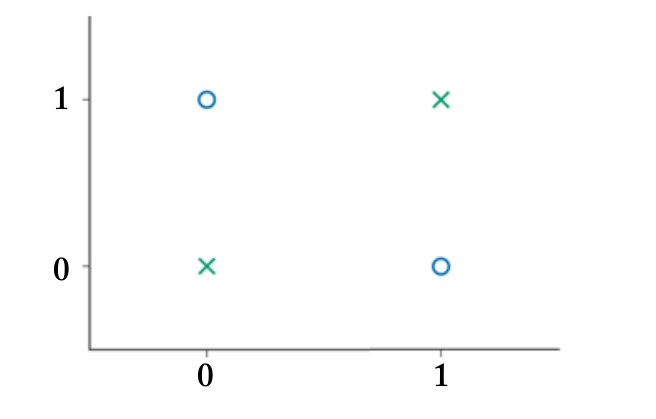
\includegraphics[scale=0.35]{pics/xor.png}
\end{figure}

Es evidente que ninguna línea recta puede separar las dos clases.


\subsection{Transformaciones no lineales de las entradas}
Si transformamos los puntos alimentándolos a través de la función no lineal $\phi(x_1,x_2) = [x_1 \times x_2, x_1 + x_2]$, el problema XOR se vuelve linealmente separable.

\begin{figure}[htb]
	\centering
	 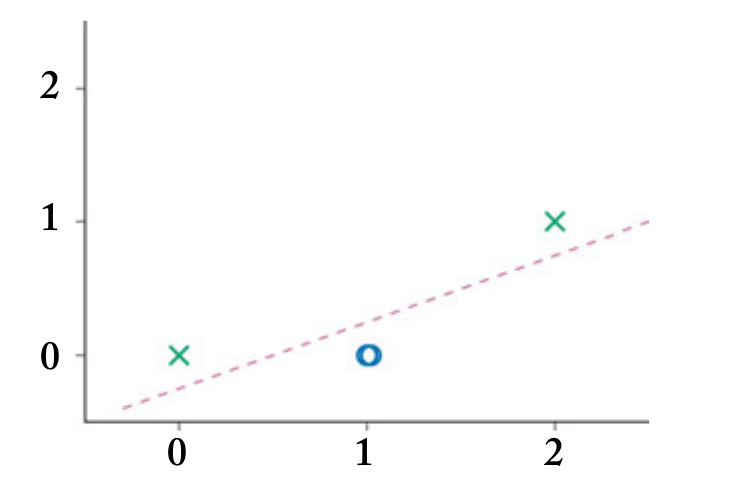
\includegraphics[scale=0.25]{pics/xor2.png}
\end{figure}

La función $\phi$ mapea los datos a una representación adecuada para la clasificación lineal. Ahora podemos entrenar fácilmente un clasificador lineal para resolver el problema XOR.

\begin{equation}
\hat{y} = f(\vec{x}) = \phi(\vec{x}) \cdot \vec{w} + b
\end{equation}

El problema es que necesitamos definir manualmente la función $\phi$. Este proceso depende del conjunto de datos particular y requiere mucha intuición humana. La sol

ción es definir una función de mapeo no lineal entrenable y entrenarla junto con el clasificador lineal. Encontrar la representación adecuada se convierte en responsabilidad del algoritmo de entrenamiento.

Las funciones de mapeo pueden tomar la forma de un modelo lineal parametrizado, seguido de una función de activación no lineal $g$ que se aplica a cada una de las dimensiones de salida:

\begin{equation}
\begin{split}
\hat{y} = f(\vec{x}) = \phi(\vec{x}) \cdot \vec{w} + b \\
\phi(\vec{x}) = g(\vec{x}W' + \vec{b}') \\
\end{split}
\end{equation}

Si tomamos $g(x) = \operatorname{max}(0, x)$ y $W' = \begin{pmatrix}
    1 & 1 \\ 1 & 1 \end{pmatrix}$, $\vec{b}' = \begin{pmatrix}
    -1 & 0 \end{pmatrix}$, obtenemos un mapeo equivalente a $[x_1 \times x_2, x_1 + x_2]$ para nuestros puntos de interés (0,0), (0,1), (1,0) y (1,1). ¡Esto resuelve con éxito el problema XOR!

Aprender tanto la función de representación como el clasificador lineal en la parte superior de ella al mismo tiempo es la idea principal detrás del aprendizaje profundo y las redes neuronales. De hecho, la ecuación anterior describe una arquitectura de red neuronal muy común llamada perceptrón multicapa (MLP, por sus siglas en inglés).



\chapter{Redes Neuronales}
\label{cap_redes}



%Translate this Latex book chapter to Spanish. Output in Latex format. Rearrange bullet points (\items) into full paragraphs. Make sure that sentences are connected in a more fluid way as they come.

\begin{itemize}
\item Las redes neuronales son una familia muy popular de modelos de aprendizaje automático formados por unidades llamadas \textbf{neuronas}.
\item Una neurona es una unidad computacional que tiene entradas y salidas escalares.
\item Cada entrada tiene asociado un peso $w$.
\item La neurona multiplica cada entrada por su peso y luego los suma (también son posibles otras funciones como \textbf{max}).
\item Aplica una función de activación $g$ (generalmente no lineal) al resultado y lo pasa a su salida.
\item Se pueden apilar múltiples capas.
\item La función de activación no lineal $g$ juega un papel crucial en la capacidad de la red para representar funciones complejas.
\item Sin la no linealidad en $g$, la red neuronal solo puede representar transformaciones lineales de la entrada.
\end{itemize}

Ejemplo: Red feedforward con dos capas

\begin{figure}[htb]
	\centering
	 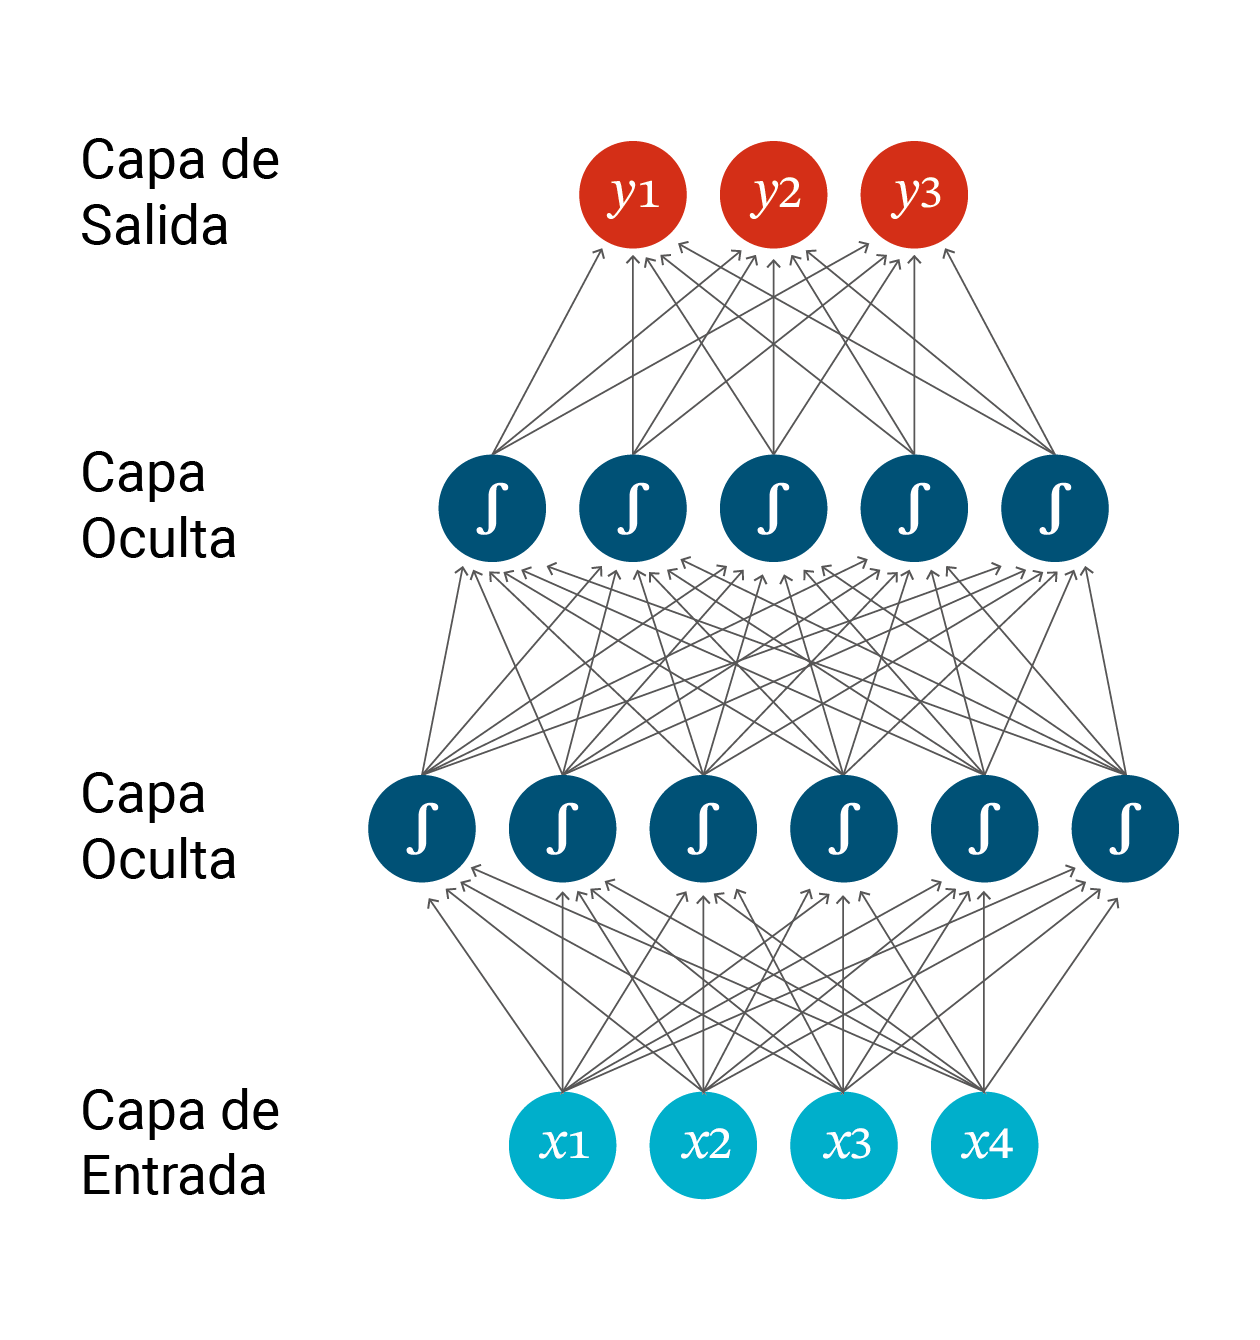
\includegraphics[scale=0.38]{pics/NN-example.png}
\end{figure}

\footnotetext{Fuente:\cite{goldberg2017neural}}

\section{Redes neuronales feedforward}

\begin{itemize}
\item La red feedforward de la imagen es una concatenación de modelos lineales separados por funciones no lineales.
\item Los valores de cada fila de neuronas en la red se pueden pensar como un vector.
\item La capa de entrada es un vector de 4 dimensiones $(\vec{x})$, y la capa superior es un vector de 6 dimensiones $(\vec{h}^1)$.
\item La capa completamente conectada se puede pensar como una transformación lineal de 4 dimensiones a 6 dimensiones.
\item Una capa completamente conectada implementa una multiplicación de vector-matriz, $\vec{h}=\vec{x}W$.
\item El peso de la conexión desde la neurona $i$-ésima en la fila de entrada hasta la neurona $j$-ésima en la fila de salida es $W_{[i,j]}$.
\item Los valores de $\vec{h}$ se transforman mediante una función no lineal $g$ que se aplica a cada valor antes de pasar al siguiente nivel.

\end{itemize}

\footnotetext{Se asume que los vectores son vectores fila y los índices en superíndices corresponden a las capas de la red.}

\paragraph{Capas completamente conectadas como multiplicaciones de vectores y matrices}
\begin{figure}[htb]
	\centering
	 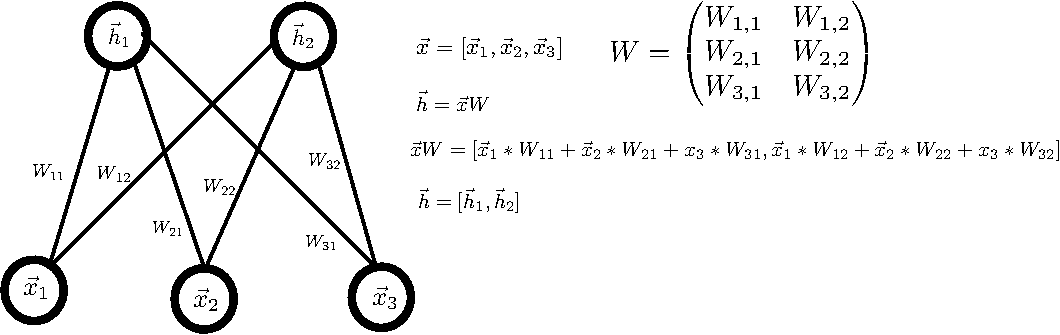
\includegraphics[scale=0.65]{pics/neural_net_mat_mul.pdf}
\end{figure}

\subsection{Redes neuronales como funciones matemáticas}

\begin{itemize}
\item El Perceptrón Multicapa (MLP, por sus siglas en inglés) de la figura se llama MLP2 porque tiene dos capas ocultas.
\item Un modelo más simple sería MLP1, un perceptrón multicapa de una capa oculta:
\begin{center}
\begin{equation}
\begin{split}
\vec{\hat{y}} = NN_{MLP1}(\vec{x}) = g(\vec{x}W^{1}+\vec{b}^{1})W^{2}+\vec{b}^{2} \\
\vec{x} \in \mathcal{R}^{in}, W^{1} \in \mathcal{R}^{d_{in}\times d_{1}}, \vec{b}^{1} \in \mathcal{R}^{d_{1}}, W^{2} \in \mathcal{R}^{d_{1}\times d_{out}}, \vec{b}^{2} \in \mathcal{R}^{d_{out}}, \vec{\hat{y}} \in \mathcal{R}^{d_{out}}
\end{split}
\end{equation}
\end{center}

\item Aquí, $W^{1}$ y $\vec{b}^{1}$ son una matriz y un término de sesgo para la primera transformación lineal de la entrada.
\item La función $g$ es una función no lineal que se aplica elemento a elemento (también se llama no linealidad o función de activación).
\item $W^{2}$ y $\vec{b}^{2}$ son la matriz y el término de sesgo para una segunda transformación lineal.

\item Al describir una red neuronal, se deben especificar las dimensiones de las capas ($d_{1}$), la entrada ($d_{in}$) y la salida ($d_{out}$).
\item MLP2 se puede escribir como la siguiente función matemática:
\begin{center}
\begin{equation}
\begin{split}
NN_{MLP2}(\vec{x}) & =  \vec{\hat{y}}  \\
\vec{h}^{1} &  = \vec{x}W^{1}+\vec{b}^{1} \\
\vec{h}^{2} &  = g^{1}(\vec{h}^{1})W^{2}+\vec{b}^{2} \\
\vec{y} &  = g^{2}(\vec{h}^{2})W^{3}\\
\vec{y} &  = (g^2(g^1(\vec{x}W^{1}+\vec{b}^{1})W^2+\vec{b}^2))W^3.\\
\end{split}
\end{equation}
\end{center}
\item Las matrices y los términos de sesgo que definen las transformaciones lineales son los parámetros de la red.
\item Al igual que en los modelos lineales, es común referirse a la colección de todos los parámetros como $\Theta$.
\end{itemize}

\section{Capacidad de representación}

\begin{itemize}
\item \cite{hornik1989multilayer} y \cite{cybenko1989approximation} mostraron que un perceptrón multicapa de una capa oculta (MLP1) es un aproximador universal.
\item MLP1 puede aproximar todas las funciones continuas en un subconjunto cerrado y acotado de $\mathcal{R}^n$.
\item Esto puede sugerir que no hay razón para ir más allá de MLP1 en arquitecturas más complejas.
\item El resultado no dice qué tan fácil o difícil es establecer los parámetros basándose en los datos de entrenamiento y un algoritmo de aprendizaje específico.
\item Tampoco garantiza que un algoritmo de entrenamiento encontrará la función correcta que genera nuestros

datos de entrenamiento.
\item Finalmente, no establece qué tan grande debería ser la capa oculta.
\item En la práctica, entrenamos redes neuronales con cantidades relativamente pequeñas de datos utilizando métodos de búsqueda local.
\item También utilizamos capas ocultas de tamaños relativamente modestos (hasta varios miles).
\item El teorema de aproximación universal no ofrece ninguna garantía bajo estas condiciones.
\item Sin embargo, definitivamente hay beneficios en probar arquitecturas más complejas que MLP1.
\item En muchos casos, sin embargo, MLP1 brinda resultados sólidos.
\end{itemize}

\section{Funciones de activación}
\begin{itemize}
\item La no linealidad $g$ puede tomar muchas formas.
\item Actualmente no existe una buena teoría sobre qué no linealidad aplicar en qué condiciones.
\item Elegir la no linealidad correcta para una tarea determinada es en su mayor parte una cuestión empírica.
\end{itemize}

\paragraph{Sigmoide}
\begin{itemize}
\item La función de activación sigmoide $\sigma(x) = \frac{1}{1+e^{-x}}$ es una función en forma de S, que transforma cada valor x en el rango $[0, 1]$.
\item El sigmoide fue la no linealidad canónica para las redes neuronales desde su inicio.
\item Actualmente se considera obsoleta para su uso en capas internas de redes neuronales, ya que las opciones que se enumeran a continuación funcionan mucho mejor empíricamente.
\end{itemize}

\begin{figure}[htb]
	\centering
	 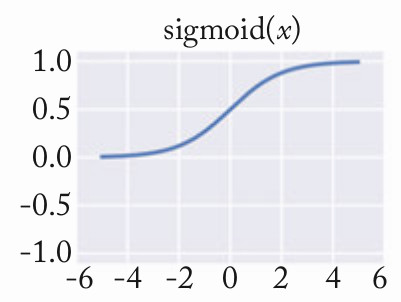
\includegraphics[scale=0.3]{pics/sigmoid2.png}
\end{figure}

\paragraph{Tangente hiperbólica (tanh)}
\begin{itemize}
\item La función de activación tangente hiperbólica $\operatorname{tanh}(x) = \frac{e^{2x}-1}{e^{2x}+1}$ es una función en forma de S que transforma los valores x en el rango $[-1, 1]$.
\end{itemize}

\begin{figure}[htb]
	\centering
	 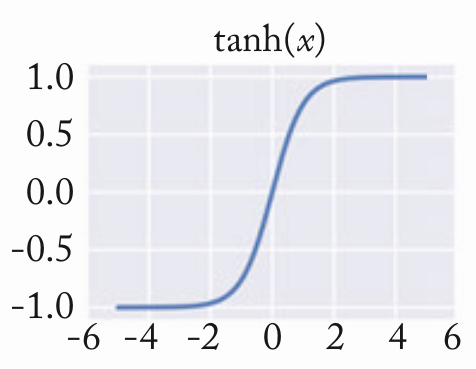
\includegraphics[scale=0.3]{pics/tanh.png}
\end{figure}

\paragraph{Hard tanh}
\begin{itemize}
\item La función de activación hard-tanh es una aproximación de la función tangente hiperbólica que es más rápida de calcular y encontrar sus derivadas:
\end{itemize}

  \[
    \operatorname{hardtanh}(x) = \left\{\begin{array}{lr}
        -1 & x < -1\\
        1 & x > 1\\
        x & \text{en otros casos.}
        \end{array} \right\}
  \]

\begin{figure}[htb]
	\centering
	 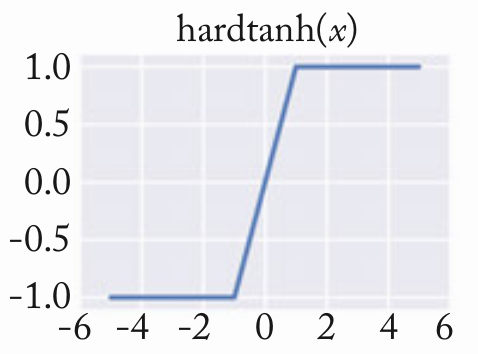
\includegraphics[scale=0.3]{pics/hardtanh.png}
\end{figure}

\paragraph{ReLU}
\begin{itemize}
\item La función de activación rectificador \cite{glorot2011deep}, también conocida como unidad lineal rectificada, es una función de activación muy simple.
\item Es fácil de trabajar y se ha demostrado muchas veces que produce excelentes resultados.
\item La

función ReLU se define como $ReLU(x) = \max(0, x)$.
\end{itemize}

\begin{figure}[htb]
	\centering
	 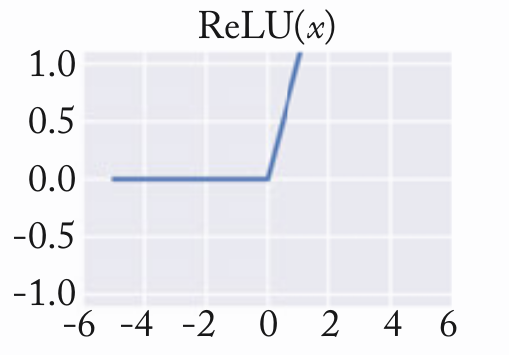
\includegraphics[scale=0.3]{pics/relu.png}
\end{figure}

\paragraph{Leaky ReLU}
\begin{itemize}
\item La función Leaky ReLU es similar a ReLU, pero permite una pequeña pendiente para valores negativos.
\item Se define como $LeakyReLU(x) = \max(\alpha x, x)$, donde $\alpha$ es un hiperparámetro pequeño (por lo general, en el rango de $0.01$ a $0.2$).
\end{itemize}

%\begin{figure}[htb]
%	\centering
%	 \includegraphics[scale=0.3]{pics/leakyrelu.png}
%\end{figure}

\paragraph{ELU}
\begin{itemize}
\item La función de activación ELU (Exponential Linear Unit) \cite{clevert2015fast} es una versión mejorada de ReLU que también tiene una pendiente para valores negativos.
\item Se define como $ELU(x) = \left\{\begin{array}{lr}
        \alpha (e^x - 1) & x < 0\\
        x & \text{en otros casos.}
        \end{array} \right\}$
\item Aquí, $\alpha$ es un hiperparámetro que controla la pendiente negativa.
\end{itemize}

%\begin{figure}[htb]
%	\centering
%	 \includegraphics[scale=0.3]{pics/elu.png}
%\end{figure}

Estas son solo algunas de las muchas opciones disponibles para las funciones de activación en redes neuronales. La elección de la función de activación puede depender del problema específico y puede requerir pruebas empíricas para determinar cuál funciona mejor.



\subsection{Problemas Prácticos}
En términos generales, tanto las unidades ReLU como las unidades tangente hiperbólica (tanh) funcionan bien y superan significativamente a la función sigmoide. Sin embargo, puede ser beneficioso experimentar con ambas activaciones, ya que cada una puede funcionar mejor en diferentes configuraciones. La Figura 1 muestra las formas de las diferentes funciones de activación, junto con las formas de sus derivadas.

\begin{figure}[htb]
	\centering
	 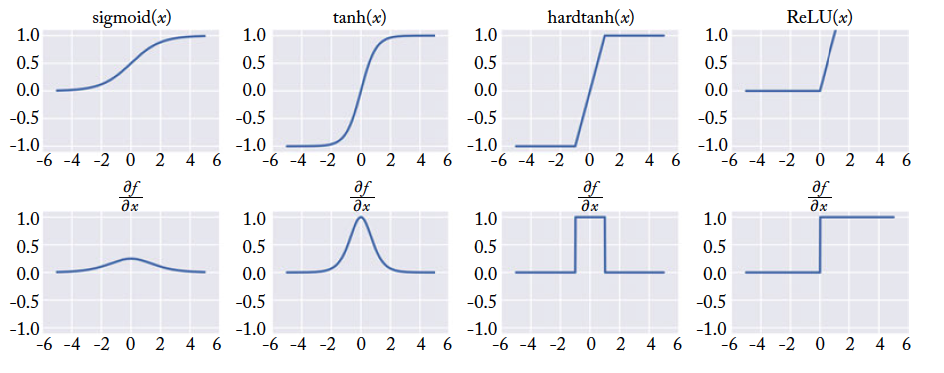
\includegraphics[scale=0.35]{pics/activations.png}
\end{figure}

\footnotetext{Fuente:\cite{goldberg2017neural}}

\section{Capas de Embedding}
En el procesamiento del lenguaje natural (PLN), la entrada a la red neuronal contiene características categóricas simbólicas (por ejemplo, palabras de un vocabulario cerrado, n-gramas de caracteres, etiquetas POS). En los modelos lineales, generalmente representamos la entrada con vectores dispersos, como la suma, el promedio o la concatenación de vectores codificados one-hot (la suma o el promedio pueden producir una representación de bolsa de palabras). En las redes neuronales, es común asociar cada valor de característica posible (es decir, cada palabra en el vocabulario, cada categoría de etiqueta POS) con un vector denso de $d$ dimensiones.

Estos vectores luego se consideran parámetros del modelo y se entrenan conjuntamente con los demás parámetros. El mapeo desde valores de características simbólicas, como "número de palabra 1249", a vectores de $d$ dimensiones se realiza mediante una capa de embedding (también llamada capa de búsqueda). Los parámetros en una capa de embedding de palabras son simplemente una matriz $E \in \mathbb{R}^{|vocab|\times d}$ donde cada fila corresponde a una palabra diferente en el vocabulario. La operación de búsqueda es simplemente una indexación: $v_{1249} = E_{[1249,:]}$. Si la característica simbólica se codifica como un vector one-hot $\vec{x}$, la operación de búsqueda se puede implementar como una multiplicación de matriz-vector $\vec{x}E$. Los vectores de embedding se combinan antes de pasar a la siguiente capa. Las operaciones comunes de combinación son concatenación, suma y promedio. Una matriz de embeddings de palabras $E$ se puede inicializar con vectores de palabras preentrenados a partir de documentos no etiquetados utilizando métodos específicos basados en la hipótesis distribucional, como los implementados en Word2Vec (que se discutirán más adelante en el curso).

\begin{figure}[htb]
	\centering
	 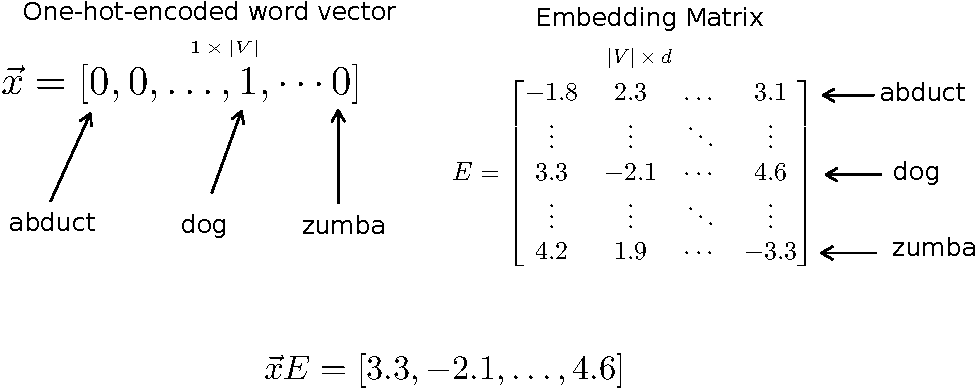
\includegraphics[scale=0.65]{pics/emb_matrix.pdf}
\end{figure}

\subsection{Vectores Densos vs Representaciones One-hot}
¿Cuáles son los beneficios de representar nuestras características como vectores en lugar de como identificadores únicos? ¿Deberíamos siempre representar las características como vectores densos? Consideremos los dos tipos de representaciones.

\begin{enumerate}
 \item \textbf{One Hot}: cada característica es su propia dimensión.
 \begin{itemize}
  \item La dimensionalidad del vector one-hot es igual al número de características distintas.
  \item  Las características son completamente independientes entre sí. La característica "la palabra es 'perro'" es tan diferente de "la palabra es 'pensando'" como lo es de "la palabra es 'gato'".
 \end{itemize}
\item \textbf{Dense}: cada característica es un vector de d dimensiones.
\begin{itemize}
 \item La dimensionalidad del vector es d.
 \item El entrenamiento del modelo hará que características similares tengan vectores similares: la información se comparte entre características similares.
\end{itemize}
\end{enumerate}




\paragraph{Ejemplo: Vectores Densos vs Representaciones One-hot}

\begin{figure}[htb]
	\centering
	 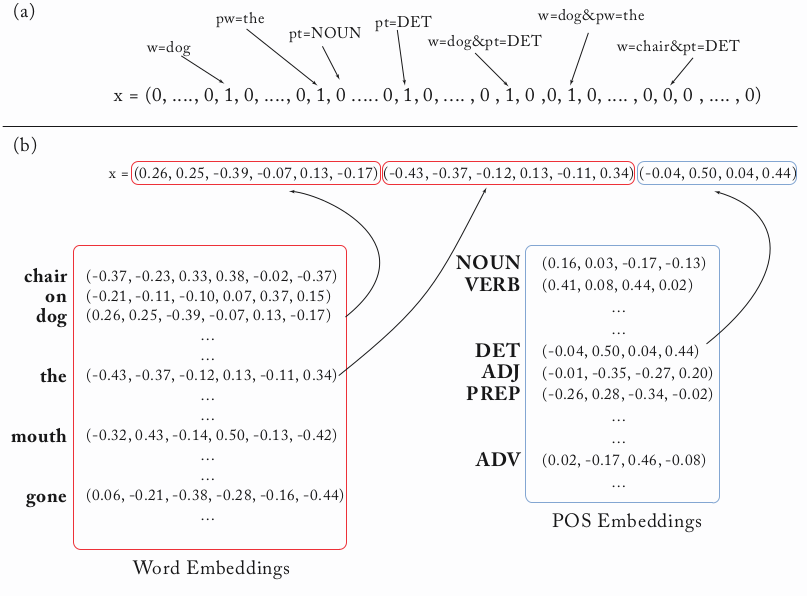
\includegraphics[scale=0.35]{pics/denseonehot.png}
\end{figure}

La figura anterior muestra dos codificaciones de la información: la palabra actual es "perro"; la palabra anterior es "el"; la etiqueta POS anterior es "DET".

(a) Vector de características dispersas:
\begin{itemize}
 \item Cada dimensión representa una característica.
\item Las combinaciones de características tienen sus propias dimensiones.
\item Los valores de las características son binarios.
\item La dimensionalidad es muy alta.
\end{itemize}


(b) Vector de características densas basado en embeddings.

\begin{itemize}
\item Cada característica principal se representa como un vector.
\item  Cada característica se corresponde con varias entradas del vector de entrada.
\item No hay una codificación explícita de combinaciones de características.
\item La dimensionalidad es baja.
\item Los mapeos de características a vectores provienen de una tabla de embeddings.
\end{itemize}


Un beneficio de usar vectores densos y de baja dimensionalidad es computacional: la mayoría de las bibliotecas de redes neuronales no funcionan bien con vectores dispersos de alta dimensionalidad. Sin embargo, este es solo un obstáculo técnico que se puede resolver con cierto esfuerzo de ingeniería.

El principal beneficio de las representaciones densas radica en el poder de generalización. Si creemos que algunas características pueden proporcionar pistas similares, vale la pena proporcionar una representación que pueda capturar estas similitudes. Supongamos que hemos observado la palabra "perro" muchas veces durante el entrenamiento, pero solo hemos observado la palabra "gato" unas pocas veces. Si cada una de las palabras se asocia con su propia dimensión (one-hot), las ocurrencias de "perro" no nos dirán nada sobre las ocurrencias de "gato". Sin embargo, en la representación de vectores densos, el vector aprendido para "perro" puede ser similar al vector aprendido para "gato". Esto permitirá que el modelo comparta fuerza estadística entre los dos eventos. Este argumento asume que hemos visto suficientes ocurrencias de la palabra "gato" como para que su vector sea similar al de "perro". Los vectores de palabras preentrenados (por ejemplo, Word2Vec, GloVe), que se discutirán más adelante en el curso, se pueden utilizar para obtener vectores densos a partir de texto no anotado.



\section{Entrenamiento de Redes Neuronales}

Las redes neuronales se entrenan de la misma manera que los modelos lineales. La salida de la red se utiliza para calcular una función de pérdida $L(\hat{y},y)$ que se minimiza en todos los ejemplos de entrenamiento utilizando descenso de gradiente. El algoritmo de retropropagación es una técnica eficiente para evaluar el gradiente de una función de pérdida $L$ en una red neuronal de alimentación directa con respecto a todos sus parámetros (Bishop, 2006). Los parámetros de la red incluyen $W^1, \vec{b}^1, \dots, W^m, \vec{b}^m$ para una red de $m$ capas. Cabe destacar que los superíndices se utilizan para denotar los índices de las capas (no exponenciación). Para simplificar, asumiremos que $L$ se calcula sobre un solo ejemplo. El desafío radica en que en las redes neuronales el número de parámetros puede ser enorme y necesitamos una forma eficiente de calcular los gradientes. La idea es aplicar la regla de la cadena de derivadas de manera inteligente.

\begin{figure}[htb]
	\centering
	 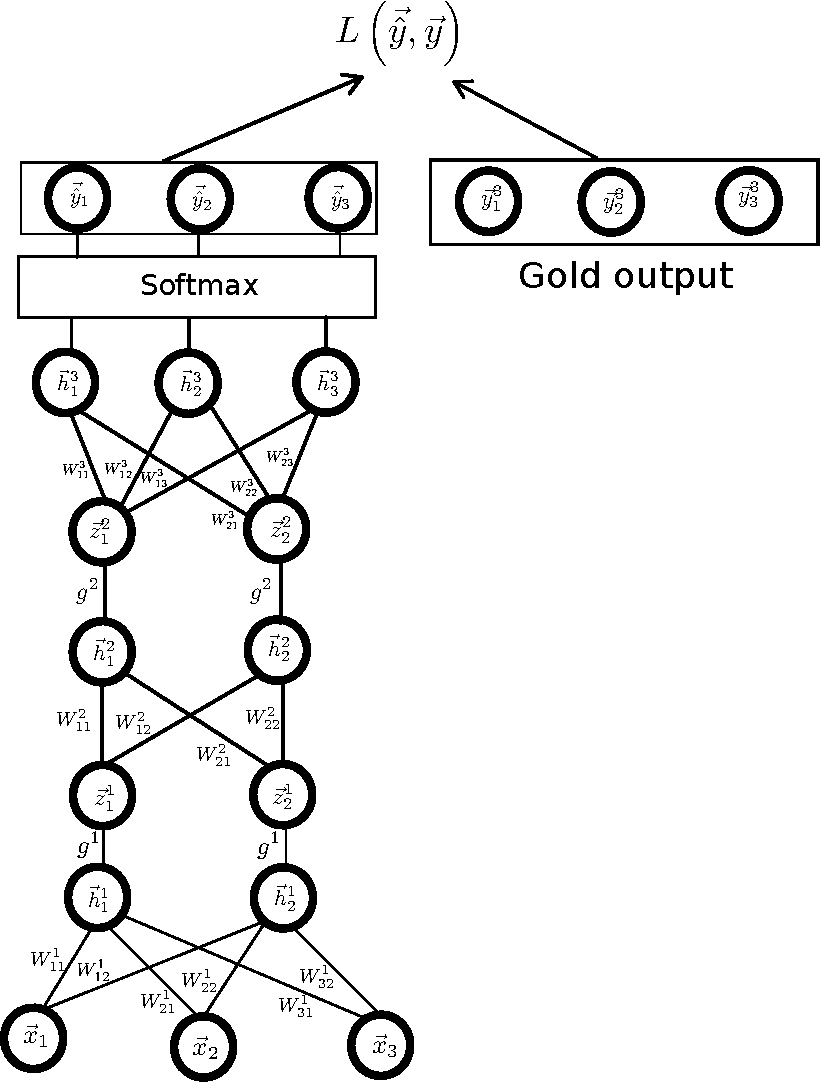
\includegraphics[scale=0.41]{pics/neural_net.pdf}
\end{figure}

\section{Recordatorio de la Regla de la Cadena en Derivadas}

La regla de la cadena simple establece que si $z = f(y)$ y $y = g(x)$, entonces

\begin{displaymath}
\frac{\partial z}{\partial x} = \frac{\partial z}{\partial y} \times \frac{\partial y}{\partial x}
\end{displaymath}

Por ejemplo, si $z= e^{y}$ y $y = 2x$, entonces

\begin{displaymath}
\frac{\partial z}{\partial x} = \frac{\partial z}{\partial y} \times \frac{\partial y}{\partial x} = e^{y} \times 2 = 2 e^{2x}
\end{displaymath}

\begin{figure}[htb]
	\centering
	 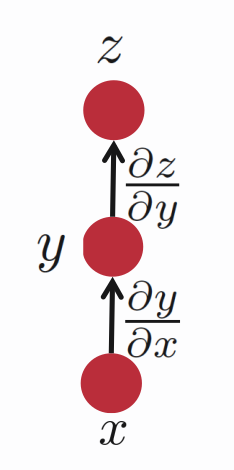
\includegraphics[scale=0.2]{pics/simple_chain_rule.png}
\end{figure}

La regla de la cadena múltiple establece que si $z = f(y_1,y_2)$, $y_1 = g_1(x)$ y $y_2 = g_2(x)$, entonces

\begin{displaymath}
\frac{\partial z}{\partial x} = \frac{\partial z}{\partial y_1} \times \frac{\partial y_1}{\partial x} + \frac{\partial z}{\partial y_2} \times \frac{\partial y_2}{\partial x}
\end{displaymath}

Por ejemplo, si $z= e^{y_1 \times y_2}$, $y_1 = 2x$ y $y_2 = x^2$, entonces

\begin{displaymath}
\frac{\partial z}{\partial x} = (e^{y_1 \times y_2}\times y_2) \times 2 + (e^{y_1 \times y_2}\times y_1) \times 2x = e^{2x^3} \times 6x^2
\end{displaymath}


\begin{figure}[htb]
	\centering
	 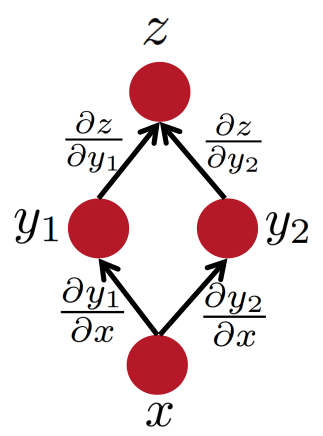
\includegraphics[scale=0.3]{pics/multiple_paths_chain_rule.png}
\end{figure}

La versión general de la regla de la cadena múltiple es:

\begin{displaymath}
 \frac{\partial z}{\partial x} = \sum_{i=1}^n \frac{\partial z}{\partial y_i} \times \frac{\partial y_i}{\partial x}
\end{displaymath}

\begin{figure}[htb]
	\centering
	 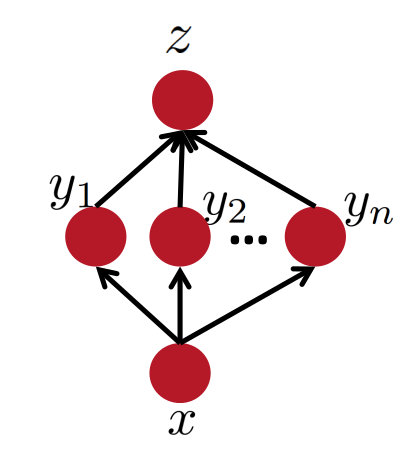
\includegraphics[scale=0.4]{pics/multiple_paths_chain_rule_general.png}
\end{figure}

\section{Retropropagación}

En una red de alimentación directa general, cada unidad calcula una suma ponderada de sus entradas de la siguiente forma:

\begin{equation}
\vec{h}_{[j]}^l = \left(\sum_{i}  W_{[i,j]}^l \times \vec{z}_{[i]}^{(l-1)}\right) + \vec{b}_{[j]}^l
\label{eq:sum}
\end{equation}

La variable $\vec{z}_{[i]}^{(l-1)}$ es una entrada que envía una conexión a la unidad $\vec{h}_{[j]}^l$, $W_{[i,j]}^l$ es el peso asociado con esa conexión, y $l$ es el índice de la capa.

Los vectores de sesgo $\vec{b}_{[j]}$ pueden excluirse de (eq. \ref{eq:sum}) e incluirse en la matriz de pesos $W_{[i,j]}^l$ al introducir una unidad adicional, o entrada, con una activación fija de +1.

Las entradas en la capa $l$, $\vec{z}_{[i]}^{(l-1)}$, son el resultado de aplicar la función de activación $g$ a las unidades de la capa anterior:

\begin{equation}
\vec{z}_{[j]}^{l} = g(\vec{h}_{[j]}^{l})
\label{eq:ac}
\end{equation}

Para la capa de entrada ($l=0$), $\vec{z}$ corresponde al vector de entrada $\vec{z} = \vec{x}$:

\begin{equation}
\vec{z}_{[j]}^0 = \vec{x}_{[j]}
\end{equation}

Para cada instancia en el conjunto de entrenamiento, proporcionamos el vector de entrada correspondiente $\vec{x}$ a la red. Luego calculamos las activaciones de todas las unidades ocultas y de salida en la red mediante la aplicación sucesiva de (eq. \ref{eq:sum}) y (eq. \ref{eq:ac}).

Este proceso a menudo se denomina propagación hacia adelante porque se puede considerar como un flujo de información hacia adelante a través de la red.

Ahora consideremos la evaluación de la derivada de $L$ con respecto a un peso $W_{[i,j]}^l$.

Suponiendo que la pérdida $L$ se calcula sobre un solo ejemplo, podemos observar que $L$ depende del peso $W_{[i,j]}^l$ únicamente a través de la suma de las entradas $\vec{h}_{[j]}^{l}$.

Por lo tanto, podemos aplicar la

regla de la cadena para derivadas parciales para obtener:

\begin{equation}
\frac{\partial L}{\partial W_{[i,j]}^l} = \frac{\partial L}{\partial \vec{h}_{[j]}^{l}} \times \frac{\partial \vec{h}_{[j]}^{l}}{\partial W_{[i,j]}^l}
\label{eq:chain}
\end{equation}

Ahora introducimos una notación útil:

\begin{equation}
\vec{\delta}_{[j]}^l \equiv \frac{\partial L}{\partial \vec{h}_{[j]}^l}
\label{eq:delta}
\end{equation}

Usando (\ref{eq:sum}), podemos escribir

\begin{equation}
\frac{\partial \vec{h}_{[j]}^l}{\partial W_{[i,j]}^l} = \vec{z}_{[i]}^{(l-1)}
\label{eq:part}
\end{equation}

Sustituyendo (\ref{eq:delta}) y (\ref{eq:part}) en (\ref{eq:chain}), obtenemos

\begin{equation}
\frac{\partial L}{\partial W_{[i,j]}^l} = \vec{\delta}_{[j]}^l \times \vec{z}_{[i]}^{(l-1)}
\label{eq:deltarule}
\end{equation}

La ecuación (\ref{eq:deltarule}) nos dice que la derivada requerida se obtiene simplemente multiplicando el valor de $\vec{\delta}_{[j]}^l$ por el valor de $\vec{z}_{[i]}^{(l-1)}$.

Por lo tanto, para evaluar las derivadas, solo necesitamos calcular el valor de $\vec{\delta}_{[j]}^l$ para cada unidad oculta y de salida en la red, y luego aplicar (\ref{eq:deltarule}) para actualizar los pesos de la red. Este proceso se conoce como retropropagación, ya que el cálculo del gradiente se propaga hacia atrás a través de la red.


Calcular $\vec{\delta}_{[j]}^m$ para las unidades de salida ($l=m$) suele ser directo, ya que las unidades de activación $\vec{h}_{[j]}^m$ se observan directamente en la expresión de pérdida.

Lo mismo se aplica a los modelos lineales poco profundos.

Para evaluar $\vec{\delta}_{[j]}^l$ para las unidades ocultas, nuevamente hacemos uso de la regla de la cadena para derivadas parciales:

\begin{equation}
\vec{\delta}_{[j]}^l \equiv \frac{\partial L}{\partial \vec{h}_{[j]}^l} = \sum_{k}\left( \frac{\partial L}{\partial \vec{h}_{[k]}^{l+1}} \times \frac{\partial \vec{h}_{[k]}^{l+1}}{\partial \vec{h}_{[j]}^l}\right)
\label{eq:deltachain}
\end{equation}

La suma se realiza sobre todas las unidades $\vec{h}_{[k]}^{l+1}$ a las que la unidad $\vec{h}_{[j]}^l$ envía conexiones.

Suponemos que las conexiones se realizan solo entre capas consecutivas en la red (desde la capa $l$ hasta la capa $(l+1)$).

Las unidades $\vec{h}_{[k]}^{l+1}$ podrían incluir otras unidades ocultas y/o unidades de salida.

Si ahora sustituimos la definición de $\vec{\delta}_{[j]}^l$ dada por la ecuación (\ref{eq:delta}) en la ecuación (\ref{eq:deltachain}), obtenemos:

\begin{equation}
\vec{\delta}_{[j]}^l \equiv \frac{\partial L}{\partial \vec{h}_{[j]}^l} = \sum_{k}\left( \vec{\delta}_{[k]}^{(l+1)}  \times \frac{\partial \vec{h}_{[k]}^{l+1}}{\partial \vec{h}_{[j]}^l} \right)
\label{eq:delta2}
\end{equation}

Ahora, para la expresión $\vec{h}_{[k]}^{l+1}$ podemos ir a su definición (ecuación \ref{eq:sum}):

\begin{displaymath}
\vec{h}_{[k]}^{(l+1)} = \left( \sum_{i} W_{[i,k]}^{l+1} \times \vec{z}_{[i]}^{l}\right) + \vec{b}_{[k]}^{(l+1)}
\end{displaymath}

Reemplazando ahora la ecuación (\ref{eq:ac}) $(\vec{z}_{[i]}^{l} = g(\vec{h}_{[i]}^{l}))$ en la ecuación anterior, obtenemos:

\begin{displaymath}
\vec{h}_{[k]}^{(l+1)} = \left( \sum_{i}   W_{[i,k]}^{l+1} \times g(\vec{h}_{[i]}^{l})\right)  + \vec{b}_{[k]}^{(l+1)}
\end{displaymath}

Al calcular $\frac{\partial \vec{h}_{[k]}^{l+1}}{\partial \vec{h}_{[j]}^l}$, todos los términos en la suma donde $i \neq j$ se cancelan.

Por lo tanto, tenemos:

\begin{equation}
\frac{\partial \vec{h}_{[k]}^{l+1}}{\partial \vec{h}_{[j]}^l} =  W_{[j,k]}^{l+1} \times g'(\vec{h}_{[j]}^{l})
\label{eq:partialhh}
\end{equation}

Sustituyendo la ecuación (\ref{eq:partialhh}) en la ecuación (\ref{eq:delta2}), obtenemos:

\begin{equation}
\vec{\delta}_{[j]}^l \equiv \frac{\partial L}{\partial \vec{h}_{[j]}^l} = \sum_{k} \left( \vec{\delta}_{[k]}^{(l+1)}  \times W_{[j,k]}^{l+1} \times g'(\vec{h}_{[j]}^{l}) \right)
\label{eq:delta3}
\end{equation}

Dado que $g'(\vec{h}_{[j]}^{l})$ no depende de $k$, podemos obtener la siguiente fórmula de retropropagación:

\begin{equation}
\vec{\delta}_{[j]}^l = g'(\vec{h}_{[j]}^{l}) \times \sum_{k} \left( \vec{\delta}_{[k]}^{(l+1)}  \times W_{[j,k]}^{l+1}\right)
\label{eq:delta4}
\end{equation}

Esto nos dice que el valor de $\vec{\delta}$ para una unidad oculta en particular se puede obtener propagando los $\vec{\delta}$ hacia atrás desde las unidades superiores en la red \cite{bishop2006pattern}.

El procedimiento de retropropagación se puede resumir de la siguiente manera:

\begin{enumerate}
  \item Aplicar un vector de entrada $\vec{x}$ a la red y propagarlo hacia adelante a través de la red utilizando las ecuaciones (\ref{eq:sum}) y (\ref{eq:ac}) para encontrar las activaciones de todas las unidades ocultas y de salida.
  \item Calcular $\vec{\delta}_{[j]}^m$ para todas las unidades de salida (recordar que las derivadas involucradas aquí son fáciles de calcular).
  \item Retropropagar los $\vec{\delta}_{[k]}^{(l+1)}$ utilizando la ecuación (\ref{eq:delta4}) para obtener $\vec{\delta}_{[j]}^l$ para cada unidad oculta en la red. Se realiza de capas superiores a capas inferiores en la red.
  \item Utilizar la ecuación (\ref{eq:deltarule}) $(\frac{\partial L}{\partial W_{[i,j]}^l} = \vec{\delta}_{[j]}^l \times \vec{z}_{[i]}^{(l-1)})$ para evaluar las derivadas requeridas.
\end{enumerate}
\section{La Abstracción del Grafo de Cómputo}
Uno puede calcular los gradientes de los varios parámetros de una red a mano e implementarlos en código. Sin embargo, este procedimiento es engorroso y propenso a errores. Por lo tanto, para la mayoría de los propósitos, es preferible utilizar herramientas automáticas para el cálculo de gradientes \cite{bengio2012practical}.

Una representación de una computación matemática arbitraria (por ejemplo, una red neuronal) como un grafo es llamada un grafo de cómputo. Esta abstracción nos permite calcular los gradientes para cualquier tipo de arquitectura de red neuronal utilizando el algoritmo de retropropagación. La formulación anterior estaba restringida a redes feedforward.

Un grafo de cómputo es un grafo dirigido acíclico (DAG, por sus siglas en inglés). Los nodos corresponden a operaciones matemáticas o variables (ligadas), y las aristas corresponden al flujo de valores intermedios entre los nodos. La estructura del grafo define el orden de la computación en términos de las dependencias entre los diferentes componentes. Dado que el resultado de una operación puede ser la entrada de varias continuaciones, el grafo es un DAG y no un árbol.

Consideremos, por ejemplo, un grafo para el cálculo de $(a*b+1)*(a*b+2)$:

\begin{figure}[htb]
	\centering
	 \includegraphics[scale=0.25]{pics/compGraph.png}
\end{figure}

La computación de $a*b$ es compartida. Dado que una red neuronal es esencialmente una expresión matemática, se puede representar como un grafo de cómputo.

La figura anterior muestra el grafo de cómputo para una MLP con una capa oculta y una transformación de salida softmax \cite{goldberg2017neural}. Los nodos ovalados representan operaciones matemáticas o funciones, y los nodos rectangulares sombreados representan parámetros (variables ligadas). Las entradas de la red se tratan como constantes y se dibujan sin un nodo circundante. Los nodos de entrada y parámetros no tienen aristas de entrada, y los nodos de salida no tienen aristas de salida. La salida de cada nodo es una matriz, cuya dimensionalidad se indica sobre el nodo.

Este grafo es incompleto: sin especificar las entradas, no podemos calcular una salida. La figura 5.1b muestra un grafo completo para una MLP que toma tres palabras como entradas y predice la distribución de etiquetas gramaticales para la tercera palabra. Este grafo se puede utilizar para la predicción, pero no para el entrenamiento, ya que la salida es un vector (no un escalar) y el grafo no tiene en cuenta la respuesta correcta ni el término de pérdida. Finalmente, el grafo en la figura 5.1c muestra el grafo de cómputo para un ejemplo de entrenamiento específico, en el cual las entradas son las (incrustaciones de) las palabras "the", "black", "dog", y la salida esperada es "NOUN" (cuyo índice es 5). El nodo de selección implementa una operación de indexación, recibiendo un vector y un índice (en este caso, 5) y devolviendo la entrada correspondiente en el vector.

\subsection{Cómputo hacia Adelante}
El paso hacia adelante (forward pass) calcula las salidas de los nodos en el grafo. Dado que la salida de cada nodo depende únicamente de sí mismo y de las aristas entrantes, es trivial calcular las salidas de todos los nodos.

Esto se hace recorriendo los nodos en un orden topológico y calculando la salida de cada nodo dado que las salidas de sus predecesores ya han sido calculadas.

Más formalmente, en un grafo de $N$ nodos, asociamos a cada nodo un índice $i$ de acuerdo con su orden topológico. Sea $f_i$ la función calculada por el nodo $i$ (por ejemplo, multiplicación, suma, etc.). Sea $\pi(i)$ los nodos padres del nodo $i$, y $\pi^{-1}(i) = \{j | i \in \pi(j)\}$ los nodos hijos del nodo $i$ (estos son los argumentos de $f_i$). Denotemos por $v(i)$ la salida del nodo $i$, es decir, la aplicación de $f_i$ a los valores de salida de sus argumentos $\pi^{-1}(i)$. Para los nodos de variables e entrada, $f_i$ es una función constante y $\pi^{-1}(i)$ está vacío. El paso hacia adelante en el grafo de cómputo calcula los valores $v(i)$ para todos los $i \in [1,N]$.

\begin{figure}[htb]
	\centering
	 \includegraphics[scale=0.35]{pics/forwardPass.png}
\end{figure}

\subsection{Cómputo hacia Atrás (Retropropagación)}
El paso hacia atrás (backward pass) comienza designando un nodo $N$ con una salida escalar $(1 \times 1)$ como nodo de pérdida y ejecutando el cómputo hacia adelante hasta ese nodo.

El cómputo hacia atrás calcula los gradientes de los parámetros con respecto al valor de ese nodo.

Denotemos por $d(i)$ la cantidad $\frac{\partial N}{\partial i}$. El algoritmo de retropropagación se utiliza para calcular los valores $d(i)$ para todos los nodos $i$.

El paso hacia atrás llena una tabla de valores $d(1), \dots, d(N)$ como se muestra en el siguiente algoritmo.

\begin{figure}[htb]
	\centering
	 \includegraphics[scale=0.35]{pics/backwardPass.png}
\end{figure}

El algoritmo de retropropagación sigue esencialmente la regla de la cadena de la diferenciación. La cantidad $\frac{\partial f_j}{\partial i}$ es la derivada parcial de $f_j(\pi^{-1}(j))$ con respecto al argumento $i \in \pi^{-1}(j)$. Este valor depende de la función $f_j$ y los valores $v(a_1), \dots, v(a_m)$ (donde $a_1, \dots, a_m = \pi^{-1}(j)$) de sus argumentos, los cuales fueron calculados en el paso hacia adelante.

Por lo tanto, para definir un nuevo tipo de nodo, es necesario definir dos métodos: uno para calcular el valor hacia adelante $v(i)$ basado en las entradas del nodo, y otro para calcular $\frac{\partial f_j}{\partial i}$ para cada $x \in \pi^{-1}(i)$.

\subsection{Resumen de la Abstracción del Grafo de Cómputo}
Observa que la formulación anterior de la retropropagación es equivalente a la dada anteriormente en clase.

La abstracción del grafo de cómputo nos permite:

\begin{enumerate}
  \item Construir fácilmente redes arbitrarias.
  \item Evaluar sus predicciones para entradas dadas (paso hacia adelante).
  \item Calcular gradientes para sus parámetros con respecto a pérdidas escalares arbitrarias (paso hacia atrás o retropropagación).
\end{enumerate}

Una propiedad interesante de la abstracción del grafo de cómputo es que nos permite calcular los gradientes para redes arbitrarias (por ejemplo, redes con conexiones saltadas, pesos compartidos, funciones de pérdida especiales, etc.).

\footnotetext{Un tutorial completo sobre el algoritmo de retropropagación sobre la abstracción del grafo de cómputo se puede encontrar aquí: \url{https://colah.github.io/posts/2015-08-Backprop/}.}

\subsection{Derivadas de funciones no matemáticas}
Definir $\frac{\partial f_j}{\partial i}$ para funciones matemáticas como $log$ o $+$ es sencillo.

Puede resultar desafiante pensar en la derivada de operaciones como pick($\vec{x},5$), que selecciona el quinto elemento de un vector.

La respuesta es pensar en términos de la contribución al cálculo. Después de seleccionar el elemento $i$-ésimo de un vector, solo ese elemento participa en el resto del cálculo.

Por lo tanto, el gradiente de pick($\vec{x},5$) es un vector $\vec{v}$ con la dimensionalidad de $\vec{x}$ donde $\vec{v}_{[5]} = 1$ y $\vec{v}_{[i \neq 5]} = 0$.

De manera similar, para la función $\max(0,x)$, el valor del gradiente es $1$ para $x > 0$ y $0$ en caso contrario.

\section{Regularización y Dropout}
Las redes de múltiples capas pueden ser grandes y tener muchos parámetros, lo que las hace especialmente propensas al sobreajuste.

La regularización del modelo es tan importante en las redes neuronales profundas como lo es en los modelos lineales, tal vez incluso más.

Las regularizaciones discutidas para modelos lineales, es decir, $L_2$, $L_1$ y la elastic-net, también son relevantes para las redes neuronales.

Otra técnica efectiva para evitar que las redes neuronales sobreajusten los datos de entrenamiento es el \textbf{dropout training} \cite{srivastava2014dropout}.

El método de dropout está diseñado para evitar que la red aprenda a depender de unidades o conexiones específicas en el proceso de entrenamiento, lo que ayuda a reducir el sobreajuste.

La idea básica detrás del dropout es apagar aleatoriamente unidades (neuronas) en cada paso de entrenamiento, lo que hace que la red aprenda a ser más robusta y generalice mejor.

El dropout  se puede aplicar a las unidades ocultas (neuronas) y/o a las conexiones entre ellas.

Durante el entrenamiento, en cada paso, se aplica una máscara binaria aleatoria a las unidades o conexiones seleccionadas para el dropout. Las unidades o conexiones que están "apagadas" tienen un valor de cero y no contribuyen al cálculo hacia adelante ni hacia atrás. Solo las unidades o conexiones "encendidas" se utilizan en el cálculo de la predicción y en la retropropagación del error.

Durante la inferencia o evaluación, no se aplica el dropout y todas las unidades o conexiones se utilizan para realizar la predicción.

Es importante destacar que el dropout no es una técnica exclusiva de las redes neuronales, pero ha demostrado ser especialmente efectiva en este contexto debido a la gran cantidad de parámetros y conexiones que suelen tener las redes neuronales profundas.

El valor típico para la tasa de dropout, es decir, la fracción de unidades o conexiones que se apagan en cada paso de entrenamiento, suele ser del orden del 0.2 al 0.5. Sin embargo, el valor óptimo puede variar según el problema y la arquitectura de la red. Por lo tanto, es recomendable experimentar con diferentes tasas de dropout para encontrar la mejor configuración para cada caso.

En resumen, la regularización y el dropout son técnicas efectivas para evitar el sobreajuste en las redes neuronales. Al utilizar regularización, como $L_2$ o $L_1$, se penalizan los grandes valores de los parámetros, lo que ayuda a controlar la complejidad del modelo. El dropout, por otro lado, apaga aleatoriamente unidades o conexiones durante el entrenamiento, lo que promueve la robustez y generalización del modelo. Ambas técnicas pueden utilizarse en conjunto para obtener mejores resultados en la generalización y evitar el sobreajuste.


%Translate this Latex book chapter to Spanish. Output in Latex format. Rearrange bullet points (\items) into full paragraphs. Make sure that sentences are connected in a more fluid way as they come.

\section{Frameworks de Aprendizaje Profundo}
Existen varios paquetes de software que implementan el modelo de grafo de cómputo. Todos estos paquetes admiten todos los componentes esenciales (tipos de nodos) para definir una amplia gama de arquitecturas de redes neuronales.

Uno de estos paquetes es \textbf{TensorFlow} (\url{https://www.tensorflow.org/}), una biblioteca de software de código abierto para cálculos numéricos utilizando gráficos de flujo de datos, desarrollada originalmente por el equipo de Google Brain.

Otro paquete popular es \textbf{Keras}, que es una API de alto nivel para redes neuronales que se ejecuta sobre TensorFlow y otros backends (\url{https://keras.io/}).

También tenemos \textbf{PyTorch}, una biblioteca de aprendizaje automático de código abierto para Python basada en Torch, desarrollada por el grupo de investigación de inteligencia artificial de Facebook. PyTorch admite la construcción de gráficos dinámicos, lo que significa que se crea un grafo de cómputo diferente desde cero para cada muestra de entrenamiento (\url{https://pytorch.org/}).


\chapter{Vectores de Palabra}
\label{cap_embeddings}
\begin{itemize}
\item A major component in neural networks for language is the use of an embedding
layer.
\item A mapping of discrete symbols to continuous vectors.
\item  When embedding words, they transform from being isolated distinct symbols into mathematical
objects that can be operated on. 
\item Distance between vectors can be equated to distance between words. 
\item This makes easier to generalize the behavior from one word to another.
\end{itemize}



\section{Distributional Vectors}
\begin{itemize}
\item \textbf{Distributional Hypothesis} \cite{harris1954}: words occurring in the same \textbf{contexts} tend to have similar meanings.
\item Or equivalently: ``a word is characterized by the \textbf{company} it keeps".
\item \textbf{Distributional representations}: words are represented by \textbf{high-dimensional vectors} based on the context's where they occur. 

\end{itemize}



\subsection{Word-context Matrices}
\begin{itemize}
\item Distributional vectors are built from word-context matrices $M$. 
\item Each cell $(i,j)$ is a co-occurrence based association value between a \textbf{target word} $w_i$ and a \textbf{context} $c_j$ calculated  from a corpus of documents.
\item Contexts are commonly defined as windows of words surrounding $w_i$.
\item The window length $k$ is a parameter ( between 1 and 8 words on both the left and the right sides of $w_i$).
\item If the Vocabulary of the target words and context words is the same, $M$ has dimensionality $|\mathcal{V}| \times |\mathcal{V}|$.
\item Whereas shorter windows are likely to capture \textbf{syntactic information} (e.g, POS), longer windows are more likely to capture topical similarity \cite{goldberg2016primer, JurafskyBook}.
\end{itemize}



Distributional Vectors with context windows of size 1


\begin{figure}[htb]
	\centering
	 \includegraphics[scale=0.3]{pics/distributionalSocher.png}
\end{figure}


\footnotetext{Example taken from:    \url{http://cs224d.stanford.edu/lectures/CS224d-Lecture2.pdf}}
%\footnote{Source: \url{http://cs224d.stanford.edu/lectures/CS224d-Lecture2.pdf}}



The associations between words and contexts can be calculated using different approaches:
\begin{enumerate}
 \item Co-occurrence counts.
\item Positive point-wise mutual information (PPMI).
\item The significance values of a paired t-test.  
\end{enumerate}

The most common of those according to \cite{JurafskyBook} is PPMI.

Distributional methods are also referred to as count-based methods.



\subsection{PPMI}
\begin{itemize}
\item  PMI calculates the log of the probability of word-context pairs occurring together over the probability of them being independent. 

\begin{equation}
 \operatorname{PMI}(w, c)= \log_2 \left( \frac{P(w,c)}{P(w)P(c)} \right) = \log_{2} \left ( \frac{\operatorname{count}(w,c)\times |D|}{\operatorname{count}(w)\times \operatorname{count}(c)} \right ) 
\end{equation}




\item Negative PMI values suggest that the pair co-occurs less often than chance. 
\item These estimates are unreliable unless the counts are calculated from very large corpora \cite{JurafskyBook}.
\item  PPMI corrects this problem by replacing negative values by zero:

\begin{equation}
 \operatorname{PPMI}(w, c)= \operatorname{max}(0,\operatorname{PMI}(w, c))
\end{equation}

\end{itemize}




\subsection{Distributed Vectors or Word embeddings}
\begin{itemize}

\item Count-based distributional vectors increase in size with vocabulary i.e., can have a very high dimensionality.

\item Explicitly storing the co-occurrence matrix can be memory-intensive. 

\item Some classification models don't scale well to high-dimensional data.

\item  The neural network community prefers using \textbf{distributed representations}\footnote{Idea: The meaning of the word is ``distributed'' over a combination of dimensions.} or \textbf{word embeddings}.

\item  Word \textbf{embeddings} are low-dimensional continuous dense word vectors trained from document corpora using \textbf{neural networks}.

\item The dimensions are not directly interpretable i.e., represent latent features of  the  word,  ``hopefully capturing useful syntactic and semantic properties''~\cite{turian2010word}.

\item They have become a crucial component of neural network architectures for NLP.

\item There are two main approaches for obtaining word embeddings:

\begin{enumerate}
\item Embedding layers: using an embedding layer in a task-specific neural network architecture trained from labeled examples (e.g., sentiment analysis).

\item Pre-trained word embeddings: creating an auxiliary predictive task from unlabeled copora (e.g., predict the following word) in which word embeddings will naturally arise from the neural-network architecture.
\end{enumerate}


\item These approaches can also be combined: one can initialize an embedding layer of a task-specific neural network with pre-trained word embeddings obtained with the second approach.


\item Most popular models based on the second approach are skip-gram \cite{Mikolov2013}, continuous bag-of-words \cite{Mikolov2013}, and Glove \cite{penningtonSM14}.

\item Word embeddings have shown to be more powerful than distributional approaches in many NLP tasks~\cite{baroni2014don}.

\item In \cite{amir2015SemEval}, they were used as \textbf{features} in a regression model for determining the association between Twitter words and \textbf{positive sentiment}. 

\end{itemize}




\section{Word2Vec}
\begin{itemize}
\item Word2Vec is a software package that implements two neural network architectures for training word embeddings:  Continuous Bag of Words (CBOW) and Skip-gram.
\item It implements two  optimization models: Negative Sampling and Hierarchical Softmax.
\item These models are shallow neural networks that are trained to predict the contexts of words.

\item A very comprehensive tutorial about the algorithms behind word2vec: \url{https://arxiv.org/pdf/1411.2738.pdf}.

\end{itemize}

 Good Word2Vec tutorial
http://mccormickml.com/2016/04/19/word2vec-tutorial-the-skip-gram-model/


\subsection{Skip-gram Model}

\begin{itemize}
\item A neural network with one ``projection'' or ``hidden'' layer is trained for predicting the words surrounding a center word, within a window  of size $k$ that is shifted along the input corpus. 
\item The center and surrounding $k$ words correspond to the input and output layers of the network.
\item Words are initially represented by 1-hot vectors: vectors of the size of the vocabulary ($|V|$) with zero values in all entries except for the corresponding word index that receives a value of 1. 
\item The output layer combines the $k$ 1-hot vectors of the surrounding words. 
\item The hidden layer has a dimensionality $d$, which determines the size of the embeddings (normally $d \ll |V|$).
\end{itemize}
  \begin{figure}[h]
        	\includegraphics[scale = 0.4]{pics/skip-gram.png}
        \end{figure}



  \begin{figure}[h]
        	\includegraphics[scale = 0.4]{pics/skip_gram_net_arch.png}
        \end{figure}
\footnotetext{Picture taken from:    \url{http://mccormickml.com/2016/04/19/word2vec-tutorial-the-skip-gram-model/}}




We use hierarchical softmax where the vocabulary is represented as a Huffman binary tree. This follows previous observations that the frequency of words works well for obtaining classes in neural net language models [16]. Huffman trees assign short binary codes to frequent words, and this further reduces the number of output units that need to be evaluated


If two different words have very similar “contexts” (that is, what words are likely to appear around them), then our model needs to output very similar results for these two words. And one way for the network to output similar context predictions for these two words is if the word vectors are similar. So, if two words have similar contexts, then our network is motivated to learn similar word vectors for these two words! Ta da!

And what does it mean for two words to have similar contexts? I think you could expect that synonyms like ``intelligent'' and ``smart'' would have very similar contexts. Or that words that are related, like ``engine'' and ``transmission'', would probably have similar contexts as well.

This can also handle stemming for you – the network will likely learn similar word vectors for the words ``ant'' and ``ants'' because these should have similar contexts.

Source: https://arxiv.org/pdf/1402.3722.pdf

\subsection{Parametrization of the Skip-gram model}

\begin{itemize}
\item  We are given an input corpus formed by a sequence of  words $w_1, w_2, w_3, . . . , w_T$ and a window size $k$.

\item We denote target or (center) words by letter $w$ and surrounding context words by letter $c$.

\item The context window $c_{1:k}$ of word $w_t$ corresponds to words $w_{t-k/2},\dots, w_{t-1}, w_{t+1}, \dots, w_{t+k/2}$ (assuming that $k$ is an even number). 

\item The objective of the Skip-gram model is to maximize the average log probability of the context words given the target words:

\begin{displaymath}
 \frac{1}{T} \sum_{t=1}^T \sum_{c \in c_{1:k}}  \log P(c|w_t)
\end{displaymath}


\item The conditional probability of a context word $c$ given a center word $w$ is modeled with a softmax ($C$ is the set of all context words, which is usually the same as the vocabulary):


\begin{displaymath}
P(c|w) = \frac{e^{\vec{c}\cdot \vec{w}}}{ \sum_{c'\in C} e^{\vec{c}'\cdot \vec{w}}}
\end{displaymath}

\item Model's parameters $\theta$: $\vec{c}$ and $\vec{w}$ (vector representations of contexts and target words).

\item Let $D$ be the set of correct word-context pairs (i.e., word pairs that are observed in the Corpus).

\item The optimization goal is to maximize the conditional log-likelihood of the contexts $c$ (this is equivalent to minimizing the cross-entropy loss):


\begin{equation}
\begin{split}
\operatorname{arg} \max_{\vec{c}, \vec{w}} & \quad \sum_{(w,c) \in D}{\log P(c|w)} = \sum_{(w,c) \in D} ( \log e^{\vec{c}\cdot \vec{w}} - \log \sum_{c'\in C} e^{\vec{c}'\cdot \vec{w}}  )
\end{split}
\end{equation}


\item Assumption: maximizing this function will result in good embeddings $\vec{w}$ i.e.,  similar words will have similar vectors.

\item The term $P(c|w)$ is computationally expensive because of the summation $\sum_{c'\in C} e^{\vec{c}'\cdot \vec{w}}$ over all the contexts $c'$.

\item Fix: replace the softmax with a hierarchical softmax (the vocabulary is represented with a Huffman binary tree). 

\item Huffman trees assign short binary codes to frequent words, reducing the number of output units to be evaluated.

\end{itemize}




The distributional hypothesis states that words in similar contexts have similar meanings. The objective above clearly tries to increase the quantity  for good word-context pairs, and decrease it for bad ones.  Intuitively, this means that words that share many contexts will be similar to each other (notealso that contexts sharing many words will also be similar to each other). This is, however, very hand-wavy.

Source: https://arxiv.org/pdf/1402.3722.pdf  

Skip-gram and Negative Sampling are not the same

\subsection{Skip-gram with Negative Sampling}
\begin{itemize}
\item Negative-sampling (NS) is presented as a more efficient model for calculating skip-gram embeddings. 
\item However, it optimizes a different objective function \cite{goldberg2014word2vec}.
\item NS maximizes the probability that a word-context pair $(w, c)$ came from the set of correct word-context pairs $D$ using a sigmoid function:

\begin{displaymath}
P(D = 1| w,c_i) = \frac{1}{1+e^{-\vec{w} \cdot \vec{c_{i}}}}
\end{displaymath}

\item Assumption: the contexts words $c_i$ are independent from each other:

\begin{displaymath}
P(D = 1| w,c_{1:k}) = \prod_{i=1}^{k}{P(D = 1| w,c_i)} = \prod_{i=1}^{k}{\frac{1}{1+e^{-\vec{w} \cdot \vec{c_{i}}}}} 
\end{displaymath}

\item This leads to the following target function (log-likelihood): 

\begin{equation}
\begin{split}
\operatorname{arg} \max_{\vec{c}, \vec{w}} & \quad \log P(D = 1| w,c_{1:k}) = \sum_{i=1}^{k}{\log \frac{1}{1+e^{-\vec{w} \cdot \vec{c_{i}}}}}
\end{split}
\end{equation}

\item This objective has a trivial solution if we set $\vec{w}$,$\vec{c}$ such that $P(D=1|w,c)=1$ for every pair $(w,c)$ from $D$.
\item This is achieved by setting $\vec{w}=\vec{c}$  and $\vec{w} \cdot \vec{c} = K$ for all $\vec{w},\vec{c}$, where $K$ is a large number.
\item We need a mechanism that prevents all the vectors from having the same value, by disallowing some $(w, c)$ combinations. 
\item One way to do so, is to present the model with some $(w, c)$ pairs for which $P(D= 1|w, c)$ must be low, i.e.
pairs which are not in the data.  
\item This is achieved sampling negative samples from $\tilde{D}$. 
\item Sample $m$ words for each word-context pair  $(w,c) \in D$.
\item Add each sampled word $w_i$ together with the original context $c$ as a negative example to $\tilde{D}$.
\item $\tilde{D}$ being $m$ times larger than $D$. 
\item The number of negative samples $m$ is a parameter of the algorithm.

\item Final objective function:
\begin{equation}
\begin{split}
\operatorname{arg} \max_{\vec{c}, \vec{w}} & \quad \sum_{(w,c) \in D}{\log P(D = 1| w,c_{1:k})} + \sum_{(w,c) \in \tilde{D}} \log P(D = 0| w,c_{1:k})
\end{split}
\end{equation}

\item The negative words are sampled from smoothed version of the corpus frequencies:
\begin{displaymath}
\frac{\#(w)^{0.75}}{\sum_{w'}\#(w')^{0.75}}
\end{displaymath}

\item This gives more relative weight to less frequent words.

\end{itemize}



\subsection{Continuous Bag of Words: CBOW}

Similar to the skip-gram model but now the center word is predicted from the surrounding context.
 \begin{figure}[h]
    	\includegraphics[scale = 0.55]{pics/CBOW.png}
    \end{figure}
       
        

\subsection{GloVe}
\begin{itemize}
\item  GloVe (from global vectors) is another popular method for training word embeddings \cite{penningtonSM14}.

\item It constructs an explicit word-context
matrix, and trains the word and context vectors $\vec{w}$ and $\vec{c}$ attempting to satisfy:

\begin{equation}
\vec{w} \cdot \vec{c} + b_{[w]}+b_{[c]} = \log \#(w,c) \quad \forall (w,c) \in D
\end{equation}

\item where $b_{[w]}$ and $b_{[c]}$ are word-specific and context-specific trained biases.

\item In terms of matrix factorization, if we fix $b_{[w]}=\log \#(w)$ and $b_{[c]}=\log \#(c)$ we'll get an objective that is very similar to factorizing the word-context PMI matrix, shifted by $\log (|D|)$.
\item In GloVe the bias parameters are learned and not fixed, giving it another degree of freedom.

\item The optimization objective is weighted least-squares loss, assigning more weight to the correct reconstruction of frequent items.
       
\item When using the same word and context vocabularies, the model suggests representing each word as the sum of its corresponding word and context embedding vectors.   
        
\end{itemize}


\section{Word Analogies}
\begin{itemize}
   
\item Word embeddings can capture certain semantic relationships, e.g. male-female, verb tense and country-capital relationships between words.

\item For example, the following relationship is found for word embeddings
trained using Word2Vec: $\vec{w}_{king} - \vec{w}_{man} + \vec{w}_{woman} \approx \vec{w}_{queen}$.

    
\end{itemize}

 \begin{figure}[h]
    	\includegraphics[scale = 0.2]{pics/linear-relationships.png}
    \end{figure}
\footnotemark{Source: \url{https://www.tensorflow.org/tutorials/word2vec}}



\section{Evaluation}
\begin{itemize}
   
\item There are many datasets with human annotated associations of word pairs or gold analogies that can be used to evaluate word embeddings algorithms.

\item Those approaches are called \textit{Intrinsic Evaluation Approaches}.

\item Most of them are implemented in: \url{https://github.com/kudkudak/word-embeddings-benchmarks}.

\item Word embeddings can also be evaluated extrinsically by using them in an external NLP task (e.g., POS tagging, sentiment analysis).

    
\end{itemize}



\section{Correspondence between Distributed and Distributional Models}
\begin{itemize}
       
\item Both the distributional ``count-based'' methods and the distributed ``neural'' ones are based on the distributional hypothesis.

\item The both attempt to capture the similarity between words based on the similarity between the contexts in which they occur.      
       
\item Levy and Goldebrg showed in \cite{levy2014neural} that Skip-gram negative sampling (SGNS) is implicitly factorizing a word-context matrix, whose cells are the pointwise mutual information (PMI) of the respective word and context pairs, shifted by a global constant. 

https://levyomer.files.wordpress.com/2014/09/neural-word-embeddings-as-implicit-matrix-factorization.pdf

\item This ties the neural methods and the traditional ``count-based'' suggesting that in a deep sense
the two algorithmic families are equivalent.
     
\end{itemize}



\section{FastText}
\begin{itemize}
  
\item FastText embeddings extend the skipgram model to take into account the internal structure of words while learning word representations \cite{bojanowski2016enriching}.

\item A vector representation is associated with each character $n$-gram.

\item  Words are represented as the sum of these representations. 

\item Taking the word \emph{where} and $n = 3$, it will be represented by the character $n$-grams: $<$wh, whe, her, ere, re$>$, and the special sequence $<$where$>$.

\item Note that the sequence \emph{$<$her$>$}, corresponding to the word ``her'' is different from the tri-gram ``her'' form the word ``here''. 

\item FastText is useful for morphologically rich languages. For example, the words ``amazing'' and ``amazingly'' share information in FastText through their shared $n$-grams, whereas in Word2Vec these two words are completely unrelated.    
  
\item Let $\mathcal{G}_{w}$ be the set of $n$-grams appearing in $w$.

\item FastText associates a vector $\vec{g}$ with each $n$-gram in $\mathcal{G}_{w}$.

\item In FastText the probability that  a word-context pair $(w, c)$ came from the input corpus $D$ is calculated as follows:

\begin{displaymath}
 P(D | w, c) = \frac{1}{1+e^{-s(w,c)}}
\end{displaymath}

where,

\begin{displaymath}
s(w,c) = \sum_{g \in {G}_{w}} \vec{g} \cdot \vec{c}.
\end{displaymath}

\item The negative sampling algorithm can be calculated in the same form as in the skip-gram model with this formulation.

\end{itemize}




\section{Sentiment-Specific Phrase Embeddings}
https://pdfs.semanticscholar.org/107f/b80ff801894b6191d0613af41aba91c134a4.pdf
\begin{itemize}
\item Problem of word embeddings: antonyms can be used in similar contexts e.g., my car is nice vs my car is ugly.

\item In \cite{TangCol14}  \textbf{sentiment-specific} word embeddings are proposed  by combining the skip-gram model with emoticon-annotated tweets :) :( .

\item These embeddings are used for \textbf{training} a word-level polarity classifier.

\item The model integrates sentiment information into the continuous representation of phrases by developing a tailored neural architecture.

\item Input: $\{w_i,s_j,pol_j\}$, where $w_i$ is a phrase (or word), $s_j$ the sentence, and $pol_j$ the sentence's polarity.

\item The training objective uses the embedding of $w_i$ to predict its context words (in the same way as the skip-gram model), and uses the sentence representation $se_j$ to predict $pol_j$.


\item Sentences ($se_j$) are represented by averaging the word vectors of their words.

\item The  objective of the sentiment part is to maximize the average of log sentiment probability: 
\begin{displaymath}
f_{sentiment}= \frac{1}{S}\sum_{j=1}^{S}\log p(pol_j|se_j)
\end{displaymath}

\item The final training objective is to maximize the linear combination of the skip-gram and sentiment objectives: 
\begin{displaymath}
f = \alpha f_{skipgram} + (1- \alpha)f_{sentiment}
\end{displaymath}

\end{itemize}


  \begin{figure}[h]
        	\includegraphics[scale = 0.4]{pics/SSPE.png}
        \end{figure}

  \begin{figure}[h]
        	\includegraphics[scale = 0.3]{pics/SSPERes.png}
        \end{figure}



\section{Gensim}
Gensim is an open source Python library for natural language processing that implements many algorithms for training word embeddings.

\begin{itemize}
 \item \url{https://radimrehurek.com/gensim/}

  \item \url{https://machinelearningmastery.com/develop-word-embeddings-python-gensim/}
 
\end{itemize}



  \begin{figure}[h]
        	\includegraphics[scale = 0.3]{pics/gensim.png}
        \end{figure}



\chapter{Etiquetado de Secuencias}
\label{cap_etisec}
%Translate this Latex book chapter to Spanish. Output in Latex format. Rearrange bullet points (\items) into full paragraphs. Make sure that sentences are connected in a more fluid way as they come. Elaborate on incomplete ideas where appropriate.

\section{Tareas de Etiquetado de Secuencias o Etiquetado}
\begin{itemize}
  \item El etiquetado de secuencias o etiquetado es una tarea en PNL que difiere de la clasificación de documentos.
  \item El objetivo es asignar etiquetas o etiquetas a una oración representada como una secuencia de tokens $x_1, x_2, \dots, x_n$.
  \item En particular, el objetivo del etiquetado de secuencias es asignar etiquetas a palabras, o más generalmente, asignar etiquetas discretas a elementos discretos en una secuencia \cite{jacobbook}.
  \item Ejemplos conocidos de esta tarea son el etiquetado de partes del discurso (POS) y el reconocimiento de entidades nombradas (NER).
\end{itemize}

\section{Etiquetado de Partes del Discurso}
\textcolor{green}{\textbf{ENTRADA:}}
Los beneficios aumentaron en Boeing Co., superando fácilmente las previsiones en Wall Street, cuando su CEO Alan Mulally anunció los resultados del primer trimestre.  \vspace{0.5cm}

\textcolor{green}{\textbf{SALIDA:}}
Los beneficios\textcolor{red}{/N} aumentaron\textcolor{red}{/V} en\textcolor{red}{/P} Boeing\textcolor{red}{/N} Co.\textcolor{red}{/N} ,\textcolor{red}{/,} superando\textcolor{red}{/V} fácilmente\textcolor{red}{/ADV} las\textcolor{red}{/DET} previsiones\textcolor{red}{/N} en\textcolor{red}{/P} Wall\textcolor{red}{/N} Street\textcolor{red}{/N} ,\textcolor{red}{/,} cuando\textcolor{red}{/P} su\textcolor{red}{/DET} CEO\textcolor{red}{/N} Alan\textcolor{red}{/N} Mulally\textcolor{red}{/N} anunció\textcolor{red}{/V} los\textcolor{red}{/DET} resultados\textcolor{red}{/N} del\textcolor{red}{/PREP} primer\textcolor{red}{/ADJ} trimestre\textcolor{red}{/N} .\textcolor{red}{/.}  \vspace{0.5cm}

\begin{itemize}
  \item \textcolor{red}{N} = \textcolor{blue}{Sustantivo}
  \item \textcolor{red}{V} = \textcolor{blue}{Verbo}
  \item \textcolor{red}{P} = \textcolor{blue}{Preposición}
  \item \textcolor{red}{Adv} = \textcolor{blue}{Adverbio}
  \item \textcolor{red}{Adj} = \textcolor{blue}{Adjetivo}
  \item ...
\end{itemize}

\begin{figure}[h]
  \includegraphics[scale=0.34]{pics/posTags.png}
\end{figure}
Fuente: \cite{JurafskyBook}

\section{Reconocimiento de Entidades Nombradas (NER)}
Una \textbf{entidad nombrada} es, hablando en términos generales, cualquier cosa a la que se puede hacer referencia con un nombre propio: una persona, un lugar, una organización. \vspace{0.5cm}

\textcolor{green}{\textbf{ENTRADA:}}
Los beneficios aumentaron en Boeing Co., superando fácilmente las previsiones en Wall Street, cuando su CEO Alan Mulally anunció los resultados del primer trimestre.  \vspace{0.5cm}

\textcolor{green}{\textbf{SALIDA:}}
Los beneficios aumentaron en \textcolor{red}{[Compañía} Boeing Co.\textcolor{red}{]}, superando fácilmente las previsiones en \textcolor{red}{[Lugar} Wall Street\textcolor{red}{]}, cuando su CEO \textcolor{red}{[Persona} Alan Mulally\textcolor{red}{]} anunció los resultados del primer trimestre. \vspace{0.5cm}

\begin{itemize}
  \item Dado que las entidades pueden abarcar varias palabras (es decir, un problema de reconocimiento de fragmentos), podemos utilizar el etiquetado BIO \cite{ramshaw1999text} para convertir el problema en un problema de etiquetado de secuencias.
  \item Etiquetado BIO: utilizar etiquetas que capturen tanto el límite como el tipo de entidad nombrada.
\end{itemize}

\paragraph{Etiquetado BIO: NER como Etiquetado de Secuencias}
\textcolor{green}{\textbf{ENTRADA:}}
Los beneficios aumentaron en Boeing Co., superando fácilmente las previsiones en Wall Street, cuando su CEO Alan Mulally anunció los resultados del primer trimestre.  \vspace{0.5cm}

\textcolor{green}{\textbf{SALIDA:}}
Los\textcolor{red}{/O} beneficios\textcolor{red}{/O} aumentaron\textcolor{red}{/O} en\textcolor{red}{/O} Boeing\textcolor{purple}{/B-C} Co.\textcolor{purple}{/I-C} ,\textcolor{red}{/O} superando\textcolor{red}{/O} fácilmente\textcolor{red}{/O} las\textcolor{red}{/O} previsiones\textcolor{red}{/O} en\textcolor{red}{/O} Wall\textcolor{purple}{/B-L} Street\textcolor{purple}{/I-L} ,\textcolor{red}{/O} cuando\textcolor{red}{/O} su\textcolor{red}{/O} CEO\textcolor{red}{/O} Alan\textcolor{purple}{/B-P} Mulally\textcolor{purple}{/I-P} anunció\textcolor{red}{/O} los\textcolor{red}{/O} resultados\textcolor{red}{/O} del\textcolor{red}{/O} primer\textcolor{red}{/O} trimestre\textcolor{red}{/O} .\textcolor{red}{/O}  \vspace{0.5cm}

\begin{itemize}
  \item \textcolor{red}{O} = \textcolor{blue}{Fuera (sin entidad)}
  \item \textcolor{purple}{B-C} = \textcolor{blue}{Comienzo de Compañía}
  \item \textcolor{purple}{I-C} = \textcolor{blue}{Dentro de Compañía}
  \item \textcolor{purple}{B-L} = \textcolor{blue}{Comienzo de Lugar}
  \item \textcolor{purple}{I-L} = \textcolor{blue}{Dentro de Lugar}
  \item \textcolor{purple}{B-P} = \textcolor{blue}{Comienzo de Persona}
  \item \textcolor{purple}{I-P} = \textcolor{blue}{Dentro de Persona}
\end{itemize}

Nuestro objetivo:
\textbf{Conjunto de entrenamiento:}
\begin{enumerate}
  \item Pierre\textcolor{red}{/NNP} Vinken\textcolor{red}{/NNP},\textcolor{red}{/,} 61\textcolor{red}{/CD} años\textcolor{red}{/NNS} de edad\textcolor{red}{/JJ},\textcolor{red}{/,} se unirá a la junta directiva como director no ejecutivo el 29 de noviembre.\textcolor{red}{/NNP}
  \item El Sr.\textcolor{red}{/NNP} Vinken\textcolor{red}{/NNP} es presidente\textcolor{red}{/NN} de Elsevier\textcolor{red}{/NNP} N.V.\textcolor{red}{/NNP}, el grupo editorial holandés.\textcolor{red}{/NNP}
  \item Rudolph\textcolor{red}{/NNP} Agnew\textcolor{red}{/NNP},\textcolor{red}{/,} de 55\textcolor{red}{/CD} años\textcolor{red}{/NNS} y presidente\textcolor{red}{/NN} de\ldots
\end{enumerate}

\subsection{Etiquetado de secuencias como aprendizaje supervisado}

\begin{itemize}
  \item Tenemos una secuencia de entradas $x = (x_1, x_2, \ldots, x_n)$ y las etiquetas correspondientes $y = (y_1, y_2, \ldots, y_n)$.
  \item La tarea consiste en aprender una función $f$ que mapea secuencias de entrada a secuencias de etiquetas: $f(x_1,x_2, \ldots, x_n) = y_1, y_2, \ldots, y_n$.
  \item Tenemos un conjunto de entrenamiento de secuencias etiquetadas: $\{(x^{(1)}, y^{(1)}), (x^{(2)}, y^{(2)}), \ldots, (x^{(m)}, y^{(m)})\}$.
\end{itemize}

\subsection{Enfoque generativo para el etiquetado de secuencias}

\begin{itemize}
  \item Los modelos generativos, como el clasificador de Naive Bayes utilizado para clasificación, también se pueden utilizar para tareas de etiquetado de secuencias en PLN.
  \item Enfoque:
  \begin{itemize}
    \item Entrenamiento: Aprender la distribución conjunta $p(x_1,x_2, \ldots, x_n,y_1, y_2, \ldots, y_n)$ de las secuencias de entrada.
    \item Decodificación: Utilizar la distribución aprendida para predecir secuencias de etiquetas para nuevas secuencias de entrada.
  \end{itemize}
  \item La decodificación en el etiquetado de secuencias implica encontrar la secuencia de etiquetas con la mayor probabilidad conjunta: $\arg\max_{y_1, y_2, \ldots, y_n}p(x_1,x_2, \ldots, x_n,y_1, y_2, \ldots, y_n)$.
\end{itemize}

\section{Modelos Ocultos de Markov}

\begin{itemize}
  \item Los Modelos Ocultos de Markov (HMM, por sus siglas en inglés) proporcionan una forma sistemática de manejar problemas de etiquetado de secuencias mediante modelos generativos y algoritmos de decodificación eficientes.
  \item Tenemos una oración de entrada $x = x_1, x_2, \ldots, x_n$ ($x_i$ es la $i$-ésima palabra en la oración).
  \item Tenemos una secuencia de etiquetas $y = y_1, y_2, \ldots, y_n$ ($y_i$ es la $i$-ésima etiqueta en la oración).
  \item Usaremos un HMM para definir $p(x_1, x_2, \ldots, x_n, y_1, y_2, \ldots, y_n)$ para cualquier oración $x_1, \ldots, x_n$ y secuencia de etiquetas $y_1, \ldots, y_n$ de la misma longitud \cite{kupiec1992robust}.
  \item Luego, la secuencia de etiquetas más probable para $x$ es:
  \[
    \arg\max_{y_1,\ldots, y_n} p(x_1, \ldots, x_n, y_1, \ldots, y_n)
  \]
\end{itemize}

\section{Modelos Ocultos de Markov Trigramas (Trigram HMM)}

Para cualquier oración $x_1, \ldots, x_n$ donde $x_i \in V$ para $i = 1, \ldots, n$, y cualquier secuencia de etiquetas $y_1, \ldots, y_{n+1}$ donde $y_i \in S$ para $i = 1, \ldots, n$, y $y_{n+1} = \text{STOP}$, la probabilidad conjunta de la oración y la secuencia de etiquetas es:
\[
  p(x_1, \ldots, x_n, y_1, \ldots, y_{n+1}) = \prod_{i=1}^{n+1} q(y_i | y_{i-2}, y_{i-1}) \prod_{i=1}^{n} e(x_i | y_i)
\]
donde hemos asumido que $x_0 = x_{-1} = *$.

\subsection{Parámetros del modelo}

\begin{itemize}
  \item $q(s|u, v)$ para cualquier $s \in S \cup \{\text{STOP}\}$, $u, v \in S \cup \{*\}$
  \begin{itemize}
    \item El valor de $q(s|u,v)$ se puede interpretar como la probabilidad de ver la etiqueta $s$ inmediatamente después del bigrama de etiquetas $(u, v)$.
  \end{itemize}
  \item $e(x|s)$ para cualquier $s \in S$, $x \in V$ 
  \begin{itemize}
    \item El valor de $e(x|s)$ se puede interpretar como la probabilidad de ver la observación $x$ emparejada con el estado $s$.
  \end{itemize}
\end{itemize}

\paragraph{Un ejemplo}

Si tenemos $n = 3$, $x_1, x_2, x_3$ igual a la oración ``the dog laughs'', y $y_1, y_2, y_3, y_4$ igual a la secuencia de etiquetas ``D N V STOP'', entonces:
\[
\begin{aligned}
p(x_1, \ldots, x_n, y_1, \ldots, y_{n+1}) = & q(D|*,*) \times q(N|*,D) \\
& \times q(V|D,N) \times q(\text{STOP}|N,V) \\
& \times e(\text{el}|D) \times e(\text{perro}|N) \times e(\text{se}|V) \times e(\text{ríe}|STOP)
\end{aligned}
\]
\begin{itemize}
  \item STOP es una etiqueta especial que termina la secuencia.
  \item Tomamos $y_0 = y_{-1} = *$, donde $*$ es un símbolo especial de "padding".
\end{itemize}

\section{Supuestos de independencia en los HMM trigramas}

\begin{itemize}
  \item Los Modelos Ocultos de Markov trigramas (HMM trigramas) se derivan

mediante la realización de supuestos específicos de independencia en el modelo.

  \item Consideremos dos secuencias de variables aleatorias: $X_1, \ldots, X_n$ y $Y_1, \ldots, Y_n$, donde $n$ es la longitud de las secuencias.

  \item Cada $X_i$ puede tomar cualquier valor en un conjunto finito $V$ de palabras, y cada $Y_i$ puede tomar cualquier valor en un conjunto finito $K$ de etiquetas posibles (por ejemplo, $K=\{D,N,V, \ldots \}$).

  \item Nuestro objetivo es modelar la probabilidad conjunta:

  \begin{align*}
    P(x_1,x_2,\dots,x_n,&y_1,\dots,y_n) \\
    &= p(y_1) \times p(y_2|y_1) \\
    &\quad \times \dots \\
    &\quad \times p(y_n|y_{n-1},y_{n-2},\dots y_1) \\
    &\quad \times p(x_1|y_{n},y_{n-1},\dots y_1) \\
    &\quad \times p(x_2|x_1,y_{n},y_{n-1},\dots y_1) \\
    &\quad \times p(x_n|x_{n-1},\dots,x_1,y_{n},y_{n-1},\dots y_1)
  \end{align*}

  \item Definimos una variable aleatoria adicional $Y_{n+1}$ que siempre toma el valor "STOP".

  \item La idea clave en los HMM es la factorización de la probabilidad conjunta:
  \[P(X_1 = x_1, \ldots, X_n = x_n, Y_1 = y_1, \ldots, Y_{n+1} = y_{n+1})\]
  \[= \prod_{i=1}^{n+1} P(Y_i = y_i | Y_{i-2} = y_{i-2}, Y_{i-1} = y_{i-1}) \times \prod_{i=1}^{n} P(X_i = x_i | Y_i = y_i)\]

  \item Primero asumimos que:
  \[P(Y_i = y_i | Y_{i-2} = y_{i-2}, Y_{i-1} = y_{i-1}) = q(y_i | y_{i-2}, y_{i-1})\]

  \item Esto asume que la secuencia $Y_1, \ldots, Y_{n+1}$ es una secuencia de Markov de segundo orden, donde cada estado depende solo de los dos estados anteriores.

  \item Y también asumimos que:
    \[P(X_i = x_i | Y_i = y_i) = e(x_i | y_i)\]

  \item Esto asume que las observaciones y los estados están condicionalmente independientes dadas las etiquetas.

\end{itemize}


\section{¿Por qué el nombre?}
\[
\begin{aligned}
  p(x_1, \ldots, x_n, y_1, \ldots, y_n) = & q(\text{STOP}|y_{n-1}, y_n) \\
  & \times \prod_{j=1}^{n} q(y_j | y_{j-2}, y_{j-1}) \\
  & \times \prod_{j=1}^{n} e(x_j | y_j)
\end{aligned}
\]
Los componentes de la cadena de Markov:
\[
q(\text{STOP}|y_{n-1}, y_n)\times \prod_{j=1}^{n} q(y_j | y_{j-2}, y_{j-1})
\]
Estas transiciones no se observan directamente para una secuencia dada de palabras $(x_1, \ldots, x_n)$, de ahí el nombre de "ocultas".

El componente observable:
\[
\prod_{j=1}^{n} e(x_j | y_j)
\]
El componente observable de los HMM modela las probabilidades de emisión de los símbolos observados ($x$) condicionados a los estados ocultos correspondientes ($y$).

\section{Estimación Suavizada}

\[
\begin{aligned}
q(Vt | DT, JJ) = & \lambda_1 \times \frac{{\text{Count}(Dt, JJ, Vt)}}{{\text{Count}(Dt, JJ)}} \\
& + \lambda_2 \times \frac{{\text{Count}(JJ, Vt)}}{{\text{Count}(JJ)}} \\
& + \lambda_3 \times \frac{{\text{Count}(Vt)}}{{\text{Count}()}}
\end{aligned}
\]

donde $\lambda_1 + \lambda_2 + \lambda_3 = 1$, y para todo $i$, $\lambda_i \geq 0$.

\vspace{0.5cm}

\[
e(\text{base} | Vt) = \frac{{\text{Count}(Vt, \text{base})}}{{\text{Count}(Vt)}}
\]

\section{Tratando con Palabras de Baja Frecuencia}

Un método común es el siguiente:
\begin{itemize}
  \item Paso 1: Dividir el vocabulario en dos conjuntos
    \begin{itemize}
      \item Palabras frecuentes = palabras que ocurren $\geq 5$ veces en el entrenamiento
      \item Palabras de baja frecuencia = todas las demás palabras
    \end{itemize}
  \item Paso 2: Mapear las palabras de baja frecuencia a un conjunto pequeño y finito, dependiendo de prefijos, sufijos, etc.
\end{itemize}

A continuación se muestra un ejemplo de clases de palabras para el reconocimiento de entidades nombradas \cite{bikelSW99}:

\[
\begin{array}{l|l|l}
  \text{Clase de palabra} & \text{Ejemplo}  & \text{Intuición} \\
  \hline
  \text{twoDigitNum} & 90 & \text{Año de dos dígitos} \\
  \text{fourDigitNum} & 1990 & \text{Año de cuatro dígitos} \\
  \text{containsdígito y letra} & A8956-67 & \text{Código de producto} \\
  \text{containsDigitAndDash} & 09-96 & \text{Fecha} \\
  \text{containsDigitAndSlash} & 11/9/89 & \text{Fecha} \\
  \text{containsDigitAndComma} & 23,000.00 & \text{Cantidad monetaria} \\
  \text{containsDigitAndPeriod} & 1.00 & \text{Cantidad monetaria, porcentaje} \\
  \text{othernum} & 456789 & \text{Otro número} \\
  \text{allCaps} & BBN & \text{Organización} \\
  \text{capPeriod} & M. & \text{Inicial de nombre de persona} \\
  \text{firstWord} & \text{Primera palabra de la oración} & \text{Sin información útil de capitalización} \\
  \text{initCap} & \text{Sally} & \text{Palabra capitalizada} \\
  \text{lowercase} & \text{can} & \text{Palabra sin capitalizar} \\
  \text{other} & , & \text{Signos de puntuación, todas las demás palabras} \\
\end{array}
\]



\section{Problema de Decodificación}
Problema de decodificación: Para una entrada $x_1 \ldots x_n$, encontrar
\[
\arg \max_{y_1 \ldots y_{n+1}} p(x_1 \ldots x_n, y_1 \ldots y_{n+1})
\]
donde $\arg \max$ se toma sobre todas las secuencias $y_1 \ldots y_{n+1}$ tales que $y_i \in S$ para $i = 1 \ldots n$, y $y_{n+1} = \text{STOP}$.

Suponemos que $p$ toma la forma:
\[
p(x_1 \ldots x_n, y_1 \ldots y_{n+1}) = \prod_{i=1}^{n+1} q(y_i|y_{i-2}, y_{i-1}) \prod_{i=1}^{n} e(x_i|y_i)
\]

Recordemos que hemos asumido en esta definición que $y_0 = y_{-1} = *$ y $y_{n+1} =$ STOP.

\subsection{Método Bruto Ingenuo}

El método bruto ingenuo para encontrar la secuencia de etiquetas con la puntuación más alta es enumerar todas las posibles secuencias de etiquetas $y_1, \ldots, y_{n+1}$, calcular su puntuación utilizando la función $p$ y seleccionar la secuencia con la puntuación más alta.

\begin{itemize}
    \item Ejemplo:
    \begin{itemize}
        \item Oración de entrada: \textit{the dog barks}
        \item Conjunto de etiquetas posibles: $K = \{D, N, V\}$
    \end{itemize}
    
    \item Enumerar todas las posibles secuencias de etiquetas:
    \begin{itemize}
        \item $D\ D\ D\ STOP$
        \item $D\ D\ N\ STOP$
        \item $D\ D\ V\ STOP$
        \item $D\ N\ D\ STOP$
        \item $D\ N\ N\ STOP$
        \item $D\ N\ V\ STOP$
        \item ...
    \end{itemize}
\end{itemize} 
  
 En este caso, hay $3^3 = 27$ secuencias posibles. Sin embargo, para oraciones más largas, este método se vuelve ineficiente.Para una oración de entrada de longitud $n$, hay $|K|^n$ secuencias posibles de etiquetas. El crecimiento exponencial hace que la búsqueda exhaustiva sea impracticable para oraciones de longitud razonable.

\section{Decodificación de Viterbi con Programación Dinámica}

El algoritmo utilizado por los HMM para realizar una decodificación eficiente se denomina decodificación de Viterbi. La decodificación de Viterbi utiliza programación dinámica, que es una técnica para resolver problemas de optimización dividiéndolos en subproblemas superpuestos. Al almacenar las soluciones a estos subproblemas en una tabla, no es necesario recalcularlos, lo que mejora considerablemente la eficiencia de los algoritmos. A continuación, mostramos cómo funciona la programación dinámica con dos ejemplos: el factorial y Fibonacci.

\paragraph{Factorial}

\begin{itemize}
    \item Implementación recursiva:
    
    \begin{lstlisting}[language=Python]
def recur_factorial(n):
    # Caso base
    if n == 1:
        return n
    else:
        return n * recur_factorial(n-1)
    \end{lstlisting}
    
    \item Implementación con programación dinámica:
    
    \begin{lstlisting}[language=Python]
def dynamic_factorial(n):
    tabla = [0 for i in range(0, n+1)]
    
    # Caso base
    tabla[0] = 1
    
    for i in range(1, len(tabla)):
        tabla[i] = i * tabla[i-1]
    
    return tabla[n]
    \end{lstlisting}
\end{itemize}

\paragraph{Fibonacci}

\begin{itemize}
    \item Implementación recursiva:
    
    \begin{lstlisting}[language=Python]
def recur_fibonacci(n):
    if n == 1 or n == 0:
        return 1
    else:
        return recur_fibonacci(n-1) + recur_fibonacci(n-2)
    \end{lstlisting}
    
    \item Implementación con programación dinámica:
    
    \begin{lstlisting}[language=Python]
def dynamic_fibonacci(n):
    tabla = [0 for i in range(0, n+1)]
    
    # Caso base
    tabla[0] = 1
    tabla[1] = 1
    
    for i in range(2, len(tabla)):
        tabla[i] = tabla[i-1] + tabla[i-2]
    
    return tabla[n]
    \end{lstlisting}
\end{itemize}

\paragraph{Complejidad}

En las implementaciones recursivas, la complejidad puede ser bastante alta debido a los cálculos repetidos de los mismos subproblemas. Sin embargo, la programación dinámica puede reducir significativamente la complejidad al almacenar las soluciones a los subproblemas en una tabla o matriz y reutilizarlas cuando sea necesario. Este enfoque elimina los cálculos redundantes y permite una computación más eficiente. En el caso de Fibonacci, la complejidad se reduce de exponencial a lineal.

\section{El Algoritmo de Viterbi}

El algoritmo de Viterbi calcula eficientemente la máxima probabilidad de una secuencia de etiquetas utilizando programación dinámica.

\textbf{Definiciones:}

\begin{itemize}
    \item Definimos $n$ como la longitud de la oración.
    \item Definimos $S_k$ para $k = -1 \ldots n$ como el conjunto de etiquetas pos

ibles en la posición $k$: $S_{-1} = S_0 = \{*\}$, $S_k = S$ para $k \in \{1 \ldots n\}$.
    \item Definimos una versión truncada de la probabilidad codificada por el HMM hasta la posición $k$, $r(y_{-1}, y_0, y_1, \ldots, y_k)$, como:
    
    \[
    r(y_{-1}, y_0, y_1, \ldots, y_k) = \prod_{i=1}^{k} q(y_i | y_{i-2}, y_{i-1})
    \]
    
    \item Definimos una tabla de programación dinámica $\pi(k, u, v)$ como la máxima probabilidad de una secuencia de etiquetas que termina en las etiquetas $u, v$ en la posición $k$:
    
    \[
    \pi(k, u, v) = \max_{y_{-1}, y_0, y_1, \ldots, y_k : y_{k-1} = u, y_k = v} r(y_{-1}, y_0, y_1, \ldots, y_k)
    \]
\end{itemize}

\paragraph{Un Ejemplo}

Recuerde que $\pi(k, u, v)$ es la máxima probabilidad de una secuencia de etiquetas que termina en las etiquetas $u, v$ en la posición $k$.

\begin{figure}[h]
    \centering
    \includegraphics[scale = 0.6]{pics/viterbi1.pdf}
\end{figure}

\begin{itemize}
    \item Hay muchas secuencias posibles de etiquetas.
    \item Cada una de ellas tiene una probabilidad calculada a partir de los parámetros $q$ y $e$.
    \item $\pi(7, P, D)$ es la máxima probabilidad de que una de estas secuencias de etiquetas termine en $P$ y $D$ en la posición $7$.
    \item La ruta representa la secuencia con la máxima probabilidad.
\end{itemize}

\subsection{Una Definición Recursiva}

\textbf{Caso base:}

\[
\pi(0, *, *) = 1
\]

\textbf{Definición recursiva:}

Para cualquier $k \in \{1 \ldots n\}$, para cualquier $u \in S_{k-1}$ y $v \in S_k$:

\[
\pi(k, u, v) = \max_{w \in S_{k-2}} (\pi(k - 1, w, u) \times q(v|w, u) \times e(x_k|v))
\]

\paragraph{Justificación de la Definición Recursiva}

Para cualquier $k \in \{1 \ldots n\}$, para cualquier $u \in S_{k-1}$ y $v \in S_k$:

\[
\pi(k, u, v) = \max_{w \in S_{k-2}} (\pi(k - 1, w, u) \times q(v|w, u) \times e(x_k|v))
\]

\begin{figure}[h]
    \centering
    \includegraphics[scale = 0.6]{pics/viterbi2.pdf}
\end{figure}



\begin{itemize}
    \item Consideremos una secuencia de etiquetas arbitraria que termina con las etiquetas $P$ y $D$ en la posición $7$.
    \item Debe contener alguna etiqueta en la posición $5$.
    \item Básicamente, estamos buscando la etiqueta que maximiza la probabilidad en la posición $5$.
\end{itemize}

\subsection{El Algoritmo de Viterbi}

\begin{algorithm}[H]
\SetKwInput{Input}{Entrada}
\SetKwInput{Initialization}{Inicialización}
\SetKwFunction{Max}{max}
\SetKwFunction{Return}{retornar}

\Input{una oración $x_1 \ldots x_n$, parámetros $q(s|u, v)$ y $e(x|s)$}

\Initialization{Establecer $\pi(0, *, *) = 1$;  $S_{-1} = S_0 = \{*\}$, $S_k = S$ para $k \in \{1 \ldots n\}$.
}

\BlankLine
\SetAlgoLined
\caption{Algoritmo de Viterbi}
\label{algo:prob_inference}
\BlankLine

\For{$k = 1$ \KwTo $n$}{
\For{$u \in S_{k-1}, v \in S_k$}{
$\pi(k, u, v) = \max_{w \in S_{k-2}} (\pi(k - 1, w, u) \times q(v|w, u) \times e(x_k|v))$
}
}

\BlankLine
\Return{$\max_{u \in S_{n-1}, v \in S_n} (\pi(n, u, v) \times q(\text{STOP}|u, v))$}
\end{algorithm}

\subsection{El Algoritmo de Viterbi con Punteros de Retroceso}

\begin{algorithm}[H]
\SetKwInput{Input}{Entrada}
\SetKwInput{Initialization}{Inicialización}
\SetKwFunction{Max}{max}
\SetKwFunction{ArgMax}{argmax}
\SetKwFunction{Return}{retornar}

\Input{una oración $x_1 \ldots x_n$, parámetros $q(s|u, v)$ y $e(x|s)$}

\Initialization{Establecer $\pi(0, *, *) = 1$;  $S_{-1} = S_0 = \{*\}$, $S_k = S$ para $k \in \{1 \ldots n\}$.
}

\BlankLine
\SetAlgoLined
\caption{Algoritmo de Viterbi con Punteros de Retroceso}
\label{algo:viterbi}
\BlankLine

\For{$k = 1$ \KwTo $n$}{
\For{$u \in S_{k-1}, v \in S_k$}{
\[
\pi(k, u, v) = \max_{w \in S_{k-2}} (\pi(k - 1, w, u) \times q(v|w, u) \times e(x_k|v))
\]    
\[
\text{bp}(k, u, v) = \arg \max_{w \in S_{k-2}} (\pi(k - 1, w, u) \times q(v|w, u) \times e(x_k|v))
    \]} 
}



\BlankLine
$(y_{n-1}, y_n) = \arg \max_{(u,v)} (\pi(n, u, v) \times q(\text{STOP}|u, v))$ \tcp*[r]{Find maximum probability and corresponding tags}
\For{$k = (n - 2)$ \KwTo $1$}{
$y_k = \text{bp}(k + 2, y_{k+1}, y_{k+2})$ \tcp*[r]{Retrieve tag sequence using backpointers}
}

\BlankLine
\Return{the tag sequence $y_1 \ldots y_n$} \tcp*[r]{Return the final tag sequence}
\end{algorithm}

En el Algoritmo \ref{algo:viterbi}, se utiliza el puntero de retroceso para reconstruir la secuencia de etiquetas con la máxima probabilidad. El algoritmo recorre las tablas $\pi$ en orden inverso, comenzando desde la posición $n$ hasta la posición $1$. En cada iteración, se elige la etiqueta $u$ y $v$ que maximizan la expresión $\pi(k, u, v) \times q(\text{STOP}|u, v)$. Estas etiquetas se agregan al comienzo de la secuencia de etiquetas $path$, y al final del algoritmo, se devuelve la secuencia $path[1:-1]$, eliminando las etiquetas de inicio y detención.

Con el algoritmo de Viterbi, podemos encontrar eficientemente la secuencia de etiquetas más probable para una oración dada, utilizando programación dinámica y aprovechando la estructura de dependencia entre las etiquetas en el HMM. Esto es especialmente útil en problemas de etiquetado de secuencias, como el etiquetado de partes del habla en NLP. 

\subsection{El Algoritmo de Viterbi: Tiempo de Ejecución}
El tiempo de ejecución del algoritmo de Viterbi se puede analizar de la siguiente manera:

\begin{itemize}
    \item Se requiere un tiempo de $O(n|S|^3)$ para calcular $q(s|u, v) \times e(x_k|s)$ para todos los valores de $k, s, u, v$.
    \item La tabla $\pi$ tiene $n|S|^2$ entradas que deben ser llenadas.
    \item Se necesita un tiempo de $O(|S|)$ para llenar una entrada.
\end{itemize}

Por lo tanto, el tiempo de ejecución total es $O(n|S|^3)$.

\paragraph{Ventajas y Desventajas}
El uso de etiquetadores basados en Modelos de Markov Ocultos (HMM) presenta ciertas ventajas y desventajas:

\begin{itemize}
    \item Los etiquetadores HMM son fáciles de entrenar (se recopilan conteos a partir de un corpus de entrenamiento).
    \item Tienen un rendimiento relativamente bueno (más del 90\% de precisión en el reconocimiento de entidades nombradas).
    \item La principal dificultad radica en modelar $e(\text{palabra} | \text{etiqueta})$, lo cual puede ser muy complejo si las "palabras" son complejas.
\end{itemize}

Aunque los etiquetadores HMM tienen ventajas en términos de simplicidad y rendimiento, la modelización de la probabilidad condicional $e(\text{palabra} | \text{etiqueta})$ puede resultar desafiante en situaciones donde las palabras son complejas o ambiguas. En tales casos, se pueden requerir técnicas más avanzadas para mejorar la precisión del etiquetado de secuencias.


\section{MEMMs}

\begin{itemize}

\item Los modelos de Markov de entropía máxima (MEMMs) utilizan modelos log-lineales multiclase para tareas de etiquetado de secuencias \cite{mccallum2000maximum}.

\item En la literatura temprana de PLN, la regresión logística a menudo se llamaba clasificación de entropía máxima \cite{jacobbook}.

\item Por lo tanto, los MEMMs se parecerán mucho a los modelos de softmax multiclase vistos en la conferencia sobre modelos lineales.

\item A diferencia de los HMM, aquí confiamos en funciones parametrizadas.

\item El objetivo de los MEMMs es modelar la siguiente distribución condicional:

\begin{displaymath}
P(s_1,s_2 \dots, s_m | x_1, \dots, x_m)
\end{displaymath}

\item Donde cada $x_j$ para $j = 1 \dots m$ es el símbolo de entrada $j$ (por ejemplo, la $j$-ésima palabra en una oración), y cada $s_j$ para $j = 1 \dots m$ es la $j$-ésima etiqueta\footnote{Estas diapositivas se basan en notas de conferencia de Michael Collins \url{http://www.cs.columbia.edu/~mcollins/crf.pdf}. La notación y la terminología se han adaptado para ser coherentes con el resto del curso.}.

\item Esperaríamos que $P$(DET, NOUN, VERB$|$the, dog, barks$)$ sea mayor que $P$(VERB, VERB, VERB$|$the, dog, barks$)$ en un modelo entrenado a partir de un conjunto de datos de entrenamiento de etiquetado POS.

\item Usamos $S$ para denotar el conjunto de etiquetas posibles.

\item Suponemos que $S$ es un conjunto finito.

\item Por ejemplo, en el etiquetado de partes del habla en inglés, $S$ sería el conjunto de todas las posibles partes del habla en inglés (sustantivo, verbo, determinante, preposición, etc.).

\item Dada una secuencia de palabras $x_1, \dots, x_m$, hay $k^m$ secuencias posibles de partes del habla $s_1, \dots, s_m$, donde $k = |S|$ es el número de partes del habla posibles.

\item Queremos estimar una distribución sobre estas $k^m$ secuencias posibles.

\item En un primer paso, los MEMMs usan la siguiente descomposición ($s_0$ siempre tiene una etiqueta especial $*$):

\begin{equation}
\begin{split}
P(s_1,s_2 \dots, s_m | x_1, \dots, x_m) \quad & = \prod_{i=1}^{m}    P(s_i | s_1 \dots, s_{i-1}, x_1, \dots, x_m)\\
\quad & = \prod_{i=1}^{m}    P(s_i | s_{i-1}, x_1, \dots, x_m)
\end{split}
\end{equation}

\item La primera igualdad es exacta (se sigue de la regla de la cadena de probabilidades condicionales).

\item La segunda igualdad se deriva de un supuesto de independencia, a saber, que para todo $i$,

\begin{displaymath}
P(s_i | s_1 \dots, s_{i-1}, x_1, \dots, x_m) = P(s_i | s_{i-1}, x_1, \dots, x_m)
\end{displaymath}

\item Por lo tanto, estamos haciendo una suposición de Markov de primer orden similar a la suposición de Markov realizada en los HMM\footnote{De hecho, hicimos una suposición de Markov de segundo orden en los HMM. Los MEMMs también se pueden extender a suposiciones de segundo orden.}.

\item La etiqueta en la posición $i$ depende solo de la etiqueta en la posición $(i-1)$.

\item Habiendo hecho estas suposiciones de independencia, luego modelamos cada término usando un modelo log-lineal multiclase (softmax):

\begin{equation}
P(s_i | s_{i-1}, x_1, \dots, x_m) = \frac{\exp (\vec{w}\cdot \vec{\phi}(x_1, \cdots, x_m, i, s_{i-1},s_i))}{\sum_{s' \in S} \exp (\vec{w}\cdot \vec{\phi}(x_1, \cdots, x_m, i, s_{i-1},s'))}
\end{equation}

\end{itemize}

Aquí, $\vec{\phi}(x_1, \cdots, x_m, i, s_{i-1},s_i)$ es un vector de características donde:
\begin{itemize}
\item $x_1, \cdots, x_m$ es la oración completa que se está etiquetando.
\item $i$ es la posición a etiquetar (puede tomar cualquier valor de $1$ a $m$).
\item $s_{i-1}$ es el valor de la etiqueta anterior (puede tomar cualquier valor en $S$).
\item $s_i$ es el nuevo valor de la etiqueta (puede tomar cualquier valor en $S$).

\end{itemize}

El alcance del vector de características está \textbf{restringido} a toda la secuencia de entrada $x_1, x_m$, y solo las etiquetas anteriores y actuales. Esta restricción permite el entrenamiento eficiente tanto de los MEMMs como de los CRFs.


\section{Ejemplo de características utilizadas en el etiquetado de partes del habla}

\begin{enumerate}
\item $\vec{\phi}(x_1, \cdots, x_m, i, s_{i-1},s_i)_{[1]}=1$ si $s_i$ = ADVERB y la palabra $x_i$ termina en ``-ly''; 0 en caso contrario. \\
Si el peso $\vec{w}_{[1]}$ asociado con esta característica es grande y positivo, entonces esta característica está diciendo básicamente que preferimos etiquetas donde las palabras que terminan en -ly se etiquetan como ADVERB.

\item $\vec{\phi}(x_1, \cdots, x_m, i, s_{i-1},s_i)_{[2]}=1$ si $i=1$, $s_i$=VERB y $x_m$= $?; 0$ en caso contrario. \\
Si el peso $\vec{w}_{[2]}$ asociado con esta característica es grande y positivo, entonces se prefieren las etiquetas que asignan VERB a la primera palabra de una pregunta (por ejemplo, "¿Es esta una oración que comienza con un verbo?").

\item $\vec{\phi}(x_1, \cdots, x_m, i, s_{i-1},s_i)_{[3]}=1$ si $s_{i-1}$=ADJECTIVE y $s_i$=NOUN; 0 en caso contrario. \\
Nuevamente, un peso positivo para esta característica significa que los adjetivos tienden a ir seguidos de sustantivos.

\item $\vec{\phi}(x_1, \cdots, x_m, i, s_{i-1},s_i)_{[4]}=1$ si $s_{i-1}$=PREPOSITION y $s_{i}$=PREPOSITION. \\
Un peso negativo $\vec{w}_{[4]}$ para esta función significaría que las preposiciones no tienden a seguir a las preposiciones.

\end{enumerate}

\footnotemark{Fuente: \url{https://blog.echen.me/2012/01/03/introduction-to-conditional-random-fields/}}



\section{Plantillas de características}

Es posible definir plantillas de características más generales que cubran unigramas, bigramas, n-gramas de palabras, así como valores de etiqueta de $s_{i-1}$ y $s_i$.

\begin{enumerate}

\item Una plantilla de características de unigramas de palabras y unigramas de etiquetas: $\vec{\phi}(x_1, \cdots, x_m, i, s_{i-1},s_i)_{[index(j,z)]}=1$ si $s_i$ = TAG$_{[j]}$ y $x_i$ = WORD$_{[z]}$; 0 en caso contrario $\forall j,z$. \\
Nótese que $j$ es un índice que abarca todas las etiquetas posibles en $S$ y $z$ es otro índice que abarca las palabras en el vocabulario $V$.

\item Una plantilla de características de bigramas de palabras y bigramas de etiquetas: $\vec{\phi}(x_1, \cdots, x_m, i, s_{i-1},s_i)_{[index(j,z,u,v)]}=1$ si $s_{i-1}$ = TAG$_{[j]}$, $s_i$ = TAG$_{[z]}$, $x_{i-1}$ = WORD$_{[u]}$ y $x_{i}$ = WORD$_{[v]}$; 0 en caso contrario $\forall j,z,u,v$.

\end{enumerate}

La función $index(j,k,...)$ asignará a cada característica diferente un índice único en el vector de características. \\
Nótese que el vector resultante tendrá una dimensión muy alta y será disperso.

\paragraph{Ejemplo}
\begin{figure}[h]
\caption{Ejemplo de características en el etiquetado de partes del habla}
\centering
\includegraphics[scale = 0.73]{pics/CRF1.pdf}
\end{figure}

\begin{figure}[h]
\caption{Ejemplo de características en el etiquetado de partes del habla (continuación)}
\centering
\includegraphics[scale = 0.6]{pics/CRF2.pdf}
\end{figure}

\section{MEMMs y Softmax Multiclase}

\begin{itemize}
\item Observemos que el modelo log-lineal mencionado anteriormente es muy similar al modelo softmax multiclase presentado en la conferencia sobre modelos lineales.

\item Un modelo log-lineal general tiene la siguiente forma:

\begin{displaymath}
P(y | x; \vec{w}) = \frac{\exp (\vec{w}\cdot \vec{\phi}(x,y))}{\sum_{y' \in Y} \exp (\vec{w}\cdot \vec{\phi}(x,y'))}
\end{displaymath}


\item Un modelo softmax multiclase tiene la siguiente forma:
\begin{equation}
\begin{split}
\hat{\vec{y}} \quad & =  \operatorname{softmax}(\vec{x} \cdot W + \vec{b})  \\
\hat{\vec{y}}_{[i]} \quad & = \frac{e^{(\vec{x} \cdot W + \vec{b})_{[i]}}}{\sum_j e^{(\vec{x} \cdot W + \vec{b})_{[j]}}}
\end{split}
\end{equation}


\item Diferencia 1: en el modelo log-lineal tenemos un vector de parámetros fijo $\vec{w}$ en lugar de tener múltiples vectores (una columna de $W$ por cada valor de clase).

\item Diferencia 2: el vector de características del modelo log-lineal $\vec{\phi}(x,y)$ incluye información de la etiqueta $y$, mientras que el vector de entrada $\vec{x}$ del modelo softmax es independiente de $y$.

\item Los modelos log-lineales permiten usar características que consideran la interacción entre $x$ e $y$ (por ejemplo, $x$ termina en ``ly'' e $y$ es un ADVERBIO).


\end{itemize}



\section{Entrenamiento de los MEMMs}

\begin{itemize}

\item Una vez que hemos definido los vectores de características $\vec{\phi}$, podemos entrenar los parámetros $\vec{w}$ del modelo de la misma manera que se entrenan los modelos lineales.

\item Establecemos la log-verosimilitud negativa como función de pérdida y optimizamos los parámetros utilizando descenso de gradiente a partir de los ejemplos de entrenamiento.

\item Esto es equivalente a usar la pérdida de entropía cruzada.

\item "Cualquier pérdida que consista en una log-verosimilitud negativa es una entropía cruzada entre la distribución empírica definida por el conjunto de entrenamiento y la distribución de probabilidad definida por el modelo" \cite{goodfellow2016deep}.

\end{itemize}


\section{Decodificación con MEMMs}

\begin{itemize}

\item El problema de decodificación es el siguiente.

\item Se nos proporciona una nueva secuencia de prueba $x_1, \dots, x_m$.

\item Nuestro objetivo es calcular la secuencia de estados más probable para esta secuencia de prueba,

\begin{equation}
\operatorname{arg} \max_{s_1,\dots,s_m} P(s_1,\dots,s_m|x_1,\dots,x_m).
\end{equation}

\item Hay $k^m$ posibles secuencias de estados, por lo que para cualquier longitud de oración razonablemente grande $m$, la búsqueda exhaustiva de todas las posibilidades no será posible.

\item Podemos usar el algoritmo de Viterbi de manera similar a como se usa para los HMM.

\item La estructura de datos básica en el algoritmo será una tabla de programación dinámica $\pi$ con entradas $\pi[j,s]$ para $j=1, \dots, m$ y $s \in S$.

\item $\pi[j,s]$ almacenará la probabilidad máxima para cualquier secuencia de estados que termine en el estado $s$ en la posición $j$.

\item Formalmente, nuestro algoritmo calculará
\begin{displaymath}
\pi[j,s] = \max_{s_1,\dots, s_{j-1}}\left(P(s | s_{j-1}, x_1, \dots, x_m) \prod_{k=1}^{j-1} P(s_k | s_{k-1}, x_1, \dots, x_m)\right)
\end{displaymath}
para todo $j = 1, \dots,m$ y para todo $s \in S$.

\end{itemize}

El algoritmo es el siguiente:

\begin{itemize}

\item Inicialización: para $s \in S$

\begin{displaymath}
\pi[1,s] = P (s | s_0,x_1,\dots,x_m)
\end{displaymath}
donde $s_0$ es un estado especial "inicial".

\item Para $j \in \{2,\dots,m\}$, $s \in \{1,\dots,k\}$

\begin{displaymath}
\pi[j,s] = \max_{s' \in S} [\pi[j-1,s'] \times P (s | s',x_1,\dots,x_m)]
\end{displaymath}


\item Finalmente, después de haber completado los valores de $\pi[j,s]$ para todos los $j, s$, podemos calcular

\begin{displaymath}
\max_{s_1,\dots,s_m} = \max_{s} \pi[m,s].
\end{displaymath}


\item El algoritmo se ejecuta en tiempo $O(mk^2)$ (es decir, lineal en la longitud de la secuencia $m$, y cuadrático en el número de etiquetas $k$).

\item Al igual que en el algoritmo de Viterbi para HMM, podemos calcular la secuencia con el puntaje más alto utilizando punteros inversos en el algoritmo de programación dinámica.

\end{itemize}




\section{Comparación entre MEMMs y HMMs}

\begin{itemize}

\item  Entonces, ¿cuál es la motivación para usar MEMMs en lugar de HMMs?

\item Observa que los algoritmos de decodificación Viterbi para los dos modelos son muy similares.

\item En MEMMs, la probabilidad asociada con cada transición de estado $s_{i-1}$ a $s_i$ es

 \begin{displaymath}
 P(s_i | s_{i-1}, x_1, \dots, x_m)  =  \frac{\exp (\vec{w}\cdot \vec{\phi}(x_1, \cdots, x_m, i, s_{i-1},s_i))}{\sum_{s' \in S} \exp (\vec{w}\cdot \vec{\phi}(x_1, \cdots, x_m, i, s_{i-1},s'))}
\end{displaymath}

\item En los HMM, la probabilidad asociada a cada transición es:

\begin{displaymath}
 P(s_i | s_{i-1}, x_1, \dots, x_m) = P(s_1|s_{i-1})P(x_i|s_i)
\end{displaymath}

\item La ventaja clave de MEMMs es que el uso de vectores de características $\vec{\phi}$ permite obtener representaciones mucho más ricas que las utilizadas en los HMM.

\item Por ejemplo, la probabilidad de transición puede ser sensible a cualquier palabra en la secuencia de entrada $x_1, \dots, x_m$.

\item Además, es muy fácil introducir características que sean sensibles a las características ortográficas (por ejemplo, prefijos o sufijos) de la palabra actual $x_i$, o de las palabras circundantes.

\item Estas características son útiles en muchas aplicaciones de PNL, y son difíciles de incorporar dentro de HMMs de una manera limpia.

\end{itemize}


\section{Campos Aleatorios Condicionales (CRFs)}

\begin{itemize}

\item Ahora pasamos a hablar de Campos Aleatorios Condicionales (CRFs) \cite{LaffertyMP01}.

\item Notación: para mayor comodidad, usaremos $x_{1:m}$ para referirnos a una secuencia de entrada $x_1, \dots, x_m$, y $s_{1:m}$ para referirnos a una secuencia de etiquetas $s_1, \dots, s_m$.

\item El conjunto de todas las etiquetas posibles es nuevamente $S$.

\item El conjunto de todas las posibles secuencias de etiquetas es $S^m$.

\item En los campos aleatorios condicionales construiremos un modelo de

\begin{displaymath}
P(s_1, \dots, s_m | x_1, \dots, x_m) = P(s_{1:m}|x_{1:m})
\end{displaymath}

\item Una primera idea clave en los CRFs será definir un vector de características que mapea una secuencia de entrada completa $x_{1:m}$ emparejada con una secuencia de etiquetas completa $s_{1:m}$ a un vector de características de $d$ dimensiones:

\begin{displaymath}
\vec{\Phi}(x_{1:m},s_{1:m}) \in \mathbb{R}^d
\end{displaymath}

\item Pronto daremos una definición concreta para $\vec{\Phi}$.
\item Por ahora, asumamos que existe alguna definición.
\item A menudo nos referiremos a $\vec{\Phi}$ como un vector de características "global".
\item Es global en el sentido de que tiene en cuenta toda la secuencia de estados.

\item En los CRFs construimos un modelo log-lineal gigante:

\begin{displaymath}
P(s_{1:m}|x_{1:m}; \vec{w}) = \frac{\exp (\vec{w} \cdot \vec{\Phi}(x_{1:m},s_{1:m}))}{\sum_{s'_{1:m} \in S^m}\exp (\vec{w} \cdot \vec{\Phi}(x_{1:m},s'_{1:m}))}
\end{displaymath}

\item Este es "solo" otro modelo log-lineal, pero es "gigante".
\item El espacio de posibles valores para $s_{1:m}$ es enorme $S^m$.
\item La constante de normalización (denominador en la expresión anterior) implica una suma sobre todas las posibles secuencias de etiquetas $S^m$.
\item Estos problemas podrían parecer causar graves problemas computacionales.
\item Bajo suposiciones apropiadas, podemos entrenar y decodificar de manera eficiente con este tipo de modelo.
\item Definimos el vector de características global $\vec{\Phi}(x_{1:m},s_{1:m})$ de la siguiente manera:

\begin{displaymath}
\vec{\Phi}(x_{1:m},s_{1:m}) = \sum_{j=1}^{m} \vec{\phi}(x_{1:m},j,s_{j-1},s_j)
\end{displaymath}

donde $\vec{\phi}(x_{1:m},j,s_{j-1},s_j)$ es igual a los vectores de características utilizados en los MEMMs.

\item Ejemplo: $\vec{\Phi}([\text{the,dog,barks}],\text{DET,NOUN,VERB}]) = \vec{\phi}([\text{the,dog,barks}],1,*,\text{DET}) + \vec{\phi}([\text{the,dog,barks}],2,\text{DET},\text{NOUN}) + \vec{\phi}([\text{the,dog,barks}],3,\text{NOUN},\text{VERB})$

\item Esencialmente, estamos sumando muchos vectores dispersos.

\end{itemize}


\paragraph{Ejemplo}
\begin{figure}[h]
\centering
\includegraphics[scale=0.26]{pics/CRF3.png}
\caption{CRF Example}
\end{figure}
\footnotemark{Fuente: \url{http://people.ischool.berkeley.edu/~dbamman/nlpF18/slides/12_neural_sequence_labeling.pdf}}


\begin{itemize}

\item Suponemos que, para cualquier dimensión de $\vec{\Phi}_{[k]}, k= 1, \dots, d$, el $k$-ésimo atributo global es:

\begin{displaymath}
\vec{\Phi}(x_{1:m},s_{1:m})_{[k]} = \sum_{j=1}^{m} \vec{\phi}(x_{1:m},j,s_{j-1},s_j)_{[k]}
\end{displaymath}

\item Por lo tanto, $\vec{\Phi}(x_{1:m},s_{1:m})_{[k]}$ se calcula sumando el vector de características "local" $\vec{\phi}(x_{1:m},j,s_{j-1},s_j)_{[k]}$ sobre las $m$ transiciones de etiquetas diferentes en $s_1,\dots,s_m$.

\item Esperaríamos que cada vector local codifique información relevante sobre la transición de etiquetas activando algunas dimensiones del vector (estableciendo el valor en uno).

\item Ahora pasamos a dos problemas prácticos críticos en los CRFs: primero, la decodificación, y segundo, la estimación de parámetros (entrenamiento).

\end{itemize}



\section{Decodificación con CRFs}

\begin{itemize}

\item El problema de decodificación en los CRFs es el siguiente.
\item Dada una secuencia de entrada $x_{1:m} = x_1, x_2, \dots, x_m$, nos gustaría encontrar la secuencia de estados subyacente más probable bajo el modelo, es decir,

\begin{equation}
\begin{split}
\operatorname{arg} \max_{s_{1:m} \in S^m} P(s_{1:m}| x_{1:m}; \vec{w}) & = \operatorname{arg} \max_{s_{1:m} \in S^m} \frac{\exp (\vec{w} \cdot \vec{\Phi}(x_{1:m},s_{1:m}))}{\sum_{s'_{1:m} \in S^m}\exp (\vec{w} \cdot \vec{\Phi}(x_{1:m},s'_{1:m}))} \\
& = \operatorname{arg} \max_{s_{1:m} \in S^m} \exp (\vec{w} \cdot \vec{\Phi}(x_{1:m},s_{1:m})) \\
& = \operatorname{arg} \max_{s_{1:m} \in S^m} \vec{w} \cdot \vec{\Phi}(x_{1:m},s_{1:m}) \\
& = \operatorname{arg} \max_{s_{1:m} \in S^m} \vec{w} \cdot \sum_{j=1}^{m} \vec{\phi}(x_{1:m},j,s_{j-1},s_j) \\
& = \operatorname{arg} \max_{s_{1:m} \in S^m} \sum_{j=1}^{m} \vec{w} \cdot \vec{\phi}(x_{1:m},j,s_{j-1},s_j)
\end{split}
\end{equation}

\item Hemos demostrado que encontrar la secuencia más probable bajo el modelo es equivalente a encontrar la secuencia que maximiza:

\begin{displaymath}
\operatorname{arg} \max_{s_{1:m} \in S^m} \sum_{j=1}^{m} \vec{w} \cdot \vec{\phi}(x_{1:m},j,s_{j-1},s_j)
\end{displaymath}

\item Este problema tiene una intuición clara. Cada transición de la etiqueta $s_{j-1}$ a la etiqueta $s_j$ tiene un puntaje asociado: $\vec{w} \cdot \vec{\phi}(x_{1:m},j,s_{j-1},s_j)$.

\item Este puntaje podría ser positivo o negativo.

\item Intuitivamente, este puntaje será relativamente alto si la transición de estados es plausible, relativamente bajo si esta transición es implausible.

\item El problema de decodificación consiste en encontrar una secuencia completa de estados tal que la suma de los puntajes de transición sea maximizada.

\item Podemos resolver este problema utilizando una variante del algoritmo de Viterbi, de manera muy similar al algoritmo de decodificación para HMM o MEMM.

\end{itemize}


\section{Estimación de Parámetros en CRFs (Entrenamiento)}

\begin{itemize}

\item Para la estimación de parámetros, asumimos que tenemos un conjunto de $n$ ejemplos etiquetados, $\{(x_{1:m}^i, s_{1:m}^i )\}_{i=1}^n$. Cada $x_{1:m}^i$ es una secuencia de entrada $x_1^i, \dots , x_m^i$ y cada $s_{1:m}^i$ es una secuencia de etiquetas $s_1^i, \dots , s_m^i$.

\item Nuevamente, establecemos la log-verosimilitud negativa (o entropía cruzada) como la función de pérdida $L$ y optimizamos los parámetros utilizando el descenso de gradiente.

\item El principal desafío aquí es que los cálculos del gradiente $\frac{\partial L}{\partial \vec{w}_{[k]}}$ implican una suma sobre $S^m$ (un conjunto muy grande que contiene todas las posibles secuencias de etiquetas).

\item Esta suma se puede calcular de manera eficiente utilizando el algoritmo de avance-atrás (Forward-backward algorithm)\footnote{\url{http://www.cs.columbia.edu/~mcollins/fb.pdf}}.

\item Este es otro algoritmo de programación dinámica que está estrechamente relacionado con el algoritmo de Viterbi.

\end{itemize}


\section{CRFs y MEMMs}

\begin{itemize}

\item Los CRFs y los MEMMs son modelos de etiquetado de secuencias discriminatorios: modelan la probabilidad condicional directamente a través de una función lineal-logarítmica multiclase parametrizada (softmax).

\item Los HMM, por otro lado, son modelos generativos.

\item En los MEMM, la normalización (denominador del softmax) es local: ocurre en cada paso de la etiqueta (la suma se realiza sobre todos los valores de etiqueta posibles $S$).

\item En los CRFs, la normalización es global: la suma se realiza sobre todas las posibles secuencias de etiquetas $S^m$.

\item Entrenar un MEMM es bastante fácil: simplemente se entrena un modelo log-lineal multiclase para una palabra dada a la etiqueta. Este clasificador se utiliza en cada paso de la palabra para predecir toda la secuencia.

\item Entrenar un CRF es más complejo. El objetivo es maximizar la log-probabilidad de la secuencia más probable.

\end{itemize}



\subsection{CRFs y MEMMs: el problema del sesgo de etiqueta}

\begin{itemize}

\item Los MEMMs terminan tomando decisiones en cada paso de manera independiente.

\item Esto lleva a un problema llamado "sesgo de etiqueta": en algunas configuraciones del espacio de etiquetas, los MEMMs esencialmente ignoran aspectos importantes del contexto.

\item Ejemplo: La etiqueta correcta del POS para la oración "will to fight" (voluntad de luchar) es "NN TO VB" \footnote{Aquí estamos utilizando el conjunto de etiquetas PENN Treebank: \url{https://www.eecis.udel.edu/~vijay/cis889/ie/pos-set.pdf}}.

\item Aquí, NN significa "sustantivo", TO significa "infinitivo a" y VB significa "forma base verbal".

\item Los modales (MD) aparecen con mucha más frecuencia al comienzo de la oración que los sustantivos (por ejemplo, en preguntas).

\item Por lo tanto, la etiqueta "MD" recibirá un puntaje más alto que la etiqueta "NN" cuando $x_0$=``will'' : $P(s_1 = MD|s_{0} = *,x_1 = \text{``will''},...) > P( s_1 = NN| s_{i-1} = *, x_1 = \text{``will''})$.

\item Pero sabemos que MD + TO es muy raro: "puede comer", "quisiera comer".

\item La palabra "to" es relativamente determinística (casi siempre tiene la etiqueta TO), por lo que no importa qué etiqueta la preceda.

\item Debido a la normalización local de los MEMMs,  $P(s_i = TO | s_{i-1}, x_1, \dots, x_i = \text{``to''}, \dots, x_n)$ siempre será 1 cuando $x_i=$ "to", independientemente del valor de $s_{i-1}$ (MD o NN).

\item Eso significa que nuestra predicción para "to" no puede ayudarnos a desambiguar "will".

\item Perdemos la información de que las secuencias MD + TO rara vez ocurren.

\item Como consecuencia, es probable que un MEMM etiquete la primera palabra como "MD".

\item Los CRFs superan este problema al realizar una normalización global: consideran el puntaje de toda la secuencia antes de normalizarlo y convertirlo en una distribución de probabilidades.

\end{itemize}


\section{Enlaces}

\begin{itemize}

\item \url{http://people.ischool.berkeley.edu/~dbamman/nlpF18/slides/11_memm_crf.pdf}

\item \url{http://people.ischool.berkeley.edu/~dbamman/nlpF18/slides/12_neural_sequence_labeling.pdf}

\item \url{https://www.depends-on-the-definition.com/sequence-tagging-lstm-crf/}

\item \url{https://www.quora.com/What-are-the-pros-and-cons-of-these-three-sequence-models-MaxEnt-Markov-Model-Conditional-random-fields-and-recurrent-neural-networks}

\item \url{https://people.cs.umass.edu/~mccallum/papers/crf-tutorial.pdf}

\item \url{http://www.davidsbatista.net/blog/2017/11/13/Conditional_Random_Fields}

\end{itemize}






\chapter{Redes Neuronales Convolucionales}
\label{cap_cnn}

\section{Redes Neuronales Convolucionales (CNN) en Procesamiento del Lenguaje Natural (PLN)}

Las redes neuronales convolucionales (CNN) se volvieron muy populares en la comunidad de visión por computadora debido a su éxito en la detección de objetos ("gato", "bicicletas") independientemente de su posición en la imagen. Estas redes identifican predictores locales indicativos en una estructura (por ejemplo, imágenes, oraciones) y los combinan para producir una representación vectorial de tamaño fijo para la estructura. En el procesamiento del lenguaje natural, la CNN captura los n-gramos que son más informativos para la tarea predictiva objetivo. Por ejemplo, en la clasificación de sentimientos, estos aspectos locales corresponden a n-gramos que transmiten sentimiento, como "no está mal" o "muy bueno". La idea fundamental de las CNN \cite{lecun1998gradient} es considerar la extracción de características y la clasificación como una tarea conjuntamente entrenada.

\section{Convolución Básica + Agrupamiento}

En el procesamiento del lenguaje natural, las oraciones suelen ser modeladas como secuencias de vectores de palabras. Estos vectores se pueden obtener a partir de incrustaciones de palabras pre-entrenadas o de una capa de incrustación. La CNN aplica funciones no lineales (aprendidas) o "filtros" que mapean ventanas de tamaño $k$ de palabras a valores escalares. Se pueden aplicar varios filtros, lo que resulta en un vector de dimensión $l$ (una dimensión por filtro). Los filtros capturan propiedades relevantes de las palabras en la ventana y corresponden a la "capa de convolución" de la red. La capa de "agrupamiento" se utiliza para combinar los vectores resultantes de las diferentes ventanas en un solo vector de dimensión $l$. Esto se logra tomando el valor máximo o el valor promedio observado en cada dimensión en las diferentes ventanas. El objetivo es capturar las características más importantes de la oración, independientemente de la posición. El vector resultante de dimensión $l$ se alimenta luego a una red que se utiliza para la predicción (por ejemplo, softmax). Los gradientes se propagan desde la pérdida de la red ajustando los parámetros del filtro. Los filtros aprenden a resaltar los aspectos de los datos (n-gramos) que son importantes para la tarea objetivo.

\begin{figure}[h]
  \centering
  \includegraphics[scale=0.28]{pics/CNN.png}
  \caption{Arquitectura básica de una CNN para procesamiento del lenguaje natural.}
  \label{fig:cnn}
  \footnotemark{Fuente: \cite{goldberg2017neural}}
\end{figure}

\section{Convoluciones 1D sobre Texto}

En el contexto del procesamiento del lenguaje natural, nos centramos en la operación de convolución unidimensional\footnote{1D se refiere a una convolución que se aplica a entradas unidimensionales como secuencias, a diferencia de las convoluciones 2D que se aplican a imágenes.}. Consideremos una secuencia de palabras $w_{1:n} = w_1, \dots, w_n$, cada una con su vector de palabras de $d_{emb}$ dimensiones correspondiente $E_{[w_i]} = \vec{w}_{i}$. Una convolución 1D de ancho $k$ funciona deslizando una ventana de tamaño $k$ sobre la oración y aplicando el mismo filtro a cada ventana en la secuencia. Un filtro es un producto escalar con un vector de pesos $\vec{u}$, seguido a menudo de una función de activación no lineal. Definimos el operador $\oplus (w_{i:i+k-1})$ como la concatenación de los vectores $\vec{w}_{i}, \dots, \vec{w}_{i+k-1}$. El vector concatenado de la ventana $i$-ésima es $\vec{x}_{i} = \oplus (w_{i:i+k-1}) = [\vec{w}_{i};\vec{w}_{i+1};\dots;\vec{w}_{i+k-1}]$, donde $x_{i} \in \mathbb{R}^{k \cdot d_{emb}}$. Luego, aplicamos el filtro a cada vector de ventana, lo que resulta en valores escalares $p_{i} = g(\vec{x}_{i} \cdot \vec{u})$, donde $p_{i} \in \mathbb{R}$. Es común usar $l$ filtros diferentes $\vec{u}_1, \dots, \vec{u}_l$, que se pueden organizar en una matriz $U$, y a menudo se agrega un vector de sesgo $\vec{b}$: $\vec{p}_{i} = g(\vec{x}_{i} \cdot U + \vec{b})$. Cada vector $\vec{p}_i$ es una colección de $l$ valores que representan (o resumen) la $i$-ésima ventana ($\vec{p}_{i} \in \mathbb{R}^l$). Idealmente, cada dimensión captura un tipo diferente de información indicativa. La idea principal detrás de la capa de convolución es aplicar la misma función parametrizada a todos los n-gramos en la secuencia, lo que crea una secuencia de $m$ vectores, cada uno representando un n-gramo particular en la secuencia. La representación es sensible a la identidad y al orden de las palabras dentro del n-gramo, pero se extraerá la misma representación para un n-gramo independientemente de su posición en la secuencia.

\section{Convoluciones Angostas vs. Amplias}

¿Cuántos vectores $\vec{p}_i$ tenemos? Para una oración de longitud $n$ con una ventana de tamaño $k$, hay $n - k + 1$ posiciones en las que se puede comenzar la secuencia. Obtenemos $n - k + 1$ vectores $\vec{p}_{1:n-k+1}$. Este enfoque se conoce como \textbf{convolución angosta}. Una alternativa es rellenar la oración con $k - 1$ palabras de relleno a cada lado, lo que resulta en $n + k + 1$ vectores $\vec{p}_{1:n+k+1}$. Esto se llama \textbf{convolución amplia}.

\section{Agrupamiento Vectorial}

Aplicar la convolución sobre el texto da como resultado $m$ vectores $\vec{p}_{1:m}$,

cada uno de los cuales es un vector $\vec{p}_i \in \mathbb{R}^l$. Estos vectores se combinan (se agrupan) en un solo vector $\vec{c} \in \mathbb{R}^l$ que representa toda la secuencia. Existen dos operaciones de agrupamiento comunes:

\begin{itemize}
  \item Max pooling: este operador toma el valor máximo en cada dimensión (es la operación de agrupamiento más común). Para cada dimensión $j$, se calcula $\vec{c}_{[j]} = \max_{1 < i \leq m} \vec{p}_{i[j]}$, donde $\vec{p}_{i[j]}$ denota la $j$-ésima componente de $\vec{p}_i$.

  \item Average pooling: este operador toma el valor promedio en cada índice. Se calcula $\vec{c} = \frac{1}{m} \sum_{i=1}^{m} \vec{p}_i$.
\end{itemize}

Idealmente, el vector $\vec{c}$ capturará la esencia de la información importante en la secuencia. La naturaleza de la información importante que debe ser codificada en el vector $\vec{c}$ depende de la tarea. Por ejemplo, si estamos realizando clasificación de sentimientos, la esencia son los n-gramos informativos que indican sentimiento. Durante el entrenamiento, el vector $\vec{c}$ se alimenta a capas de red adicionales (por ejemplo, una capa de perceptrón multicapa), culminando en una capa de salida que se utiliza para la predicción. El procedimiento de entrenamiento de la red calcula la pérdida con respecto a la tarea de predicción, y los gradientes de error se propagan hacia atrás a través de las capas de agrupamiento y convolución, así como a través de las capas de incrustación. El proceso de entrenamiento ajusta la matriz de convolución $U$, el vector de sesgo $\vec{b}$, la red posterior y potencialmente también la matriz de incrustación $E$\footnote{Algunas personas dejan fija la capa de incrustación durante el entrenamiento, mientras que otros permiten que los parámetros cambien.} de manera que el vector $\vec{c}$ resultante del proceso de convolución y agrupamiento realmente codifique información relevante para la tarea en cuestión.

\section{Clasificación de Sentimientos en Twitter con CNN}

En \cite{Severyn2015} se desarrolla una arquitectura de red neuronal convolucional para la clasificación de sentimientos en Twitter. Cada tweet se representa como una matriz cuyas columnas corresponden a las palabras en el tweet, preservando el orden en el que aparecen. Las palabras se representan mediante vectores densos o incrustaciones entrenadas a partir de un gran corpus de tweets no etiquetados utilizando word2vec. La red está formada por las siguientes capas: una capa de entrada con la matriz de tweets dada, una única capa de convolución, una función de activación lineal rectificada (ReLU), una capa de agrupamiento máximo (max pooling) y una capa de clasificación softmax. Los pesos de la red neuronal se pre-entrenan utilizando datos con anotaciones de emoticonos y luego se entrenan con los tweets anotados a mano del concurso SemEval. Los resultados experimentales muestran que la fase de pre-entrenamiento permite una inicialización adecuada de los pesos de la red y, por lo tanto, tiene un impacto positivo en la precisión de la clasificación.

\begin{figure}[h]
  \centering
  \includegraphics[scale=0.45]{pics/cnn-twitter.png}
  \caption{Arquitectura CNN para la clasificación de sentimientos en Twitter.}
  \label{fig:cnn-twitter}
\end{figure}

\section{Redes Neuronales Convolucionales Muy Profundas para la Clasificación de Texto}

Las arquitecturas de CNN para PLN son bastante superficiales en comparación con las redes neuronales convolucionales profundas que han impulsado el estado del arte en visión por computadora. En \cite{conneau2017very} se propone una arquitectura de red neuronal para el procesamiento de texto (VDCNN) que opera directamente a nivel de caracteres y utiliza solo convoluciones pequeñas y operaciones de agrupamiento. En lugar de utilizar incrustaciones de palabras, se utilizan incrustaciones de nivel de caracteres. Los caracteres son la representación atómica más baja del texto. El rendimiento de este modelo aumenta con la profundidad: utilizando hasta 29 capas de convolución, los autores informan mejoras sobre el estado del arte en varias tareas públicas de clasificación de texto. Las mejoras más notables se logran en conjuntos de datos grandes. Este fue uno de los primeros trabajos que mostró los beneficios de las arquitecturas neuronales profundas para PLN.

\begin{figure}[h]
  \centering
  \includegraphics[scale=0.2]{pics/VDCNN.png}
  \caption{Arquitectura VDCNN para la clasificación de texto.}
  \label{fig:vdcnn}
\end{figure}




\chapter{Redes Neuronales Recurrentes}
\label{cap_rnn}
%\begin{itemize}

\item While representations derived from convolutional networks  offer some sensitivity to word order, their order sensitivity is restricted to mostly local patterns, and disregards the order of patterns that are far apart in the sequence.
\item Recurrent neural networks (RNNs) allow representing arbitrarily sized sequential inputs in fixed-size vectors, while paying attention to the structured properties of the inputs \cite{goldberg2016primer}.
\item RNNs, particularly ones with gated architectures such as the LSTM and the GRU, are very powerful at capturing statistical regularities in sequential inputs.

\end{itemize}



\section{The RNN Abstraction}
\begin{itemize}

\item We use $\vec{x}_{i:j}$ to denote the sequence of vectors $\vec{x}_i, \dots, \vec{x}_j$.

\item On a high-level, the RNN is a function that takes as input an arbitrary length ordered sequence of $n$ $d_{in}$-dimensional vectors $\vec{x}_{1 :n}=\vec{x}_1,\vec{x}_2, \dots, \vec{x}_n$ ( $\vec{x}_i \in  \mathcal{R}^{d_{in}}$) and returns as output a single $d_{out}$ dimensional vector $\vec{y}_n$ $\in \mathcal{R}^{d_{out}}$:

\begin{equation}
\begin{split}
\vec{y}_n & = RNN(\vec{x}_{1:n}) \\
\vec{x}_i \in  \mathcal{R}^{d_{in}} & \quad  \vec{y}_n  \in \mathcal{R}^{d_{out}}
\end{split}
\end{equation}

\item This implicitly defines an output vector $\vec{y}_i$ for each prefix $\vec{x}_{1:i}$ of the sequence $\vec{x}_{i:n}$.
\item We denote by $RNN^{*}$ the function returning this sequence:
\begin{equation}
\begin{split}
\vec{y}_{1:n} & = RNN^{*}(\vec{x}_{1:n}) \\
\vec{y}_i & = RNN(\vec{x}_{1:i}) \\
\vec{x}_i \in  \mathcal{R}^{d_{in}} & \quad  \vec{y}_n  \in \mathcal{R}^{d_{out}}
\end{split}
\end{equation}
\item The output vector $\vec{y}_n$ is then used for further prediction.
\item For example, a model for predicting the conditional probability of an event $e$ given the sequence $\vec{x}_{1:n}$ can be defined as the $j$-th element in the output vector resulting from the softmax operation over a linear transformation of the RNN encoding:
\begin{displaymath}
p(e = j|\vec{x}_{1:n}) = \text{softmax}(RNN(\vec{x}_{1:n})\cdot W +\vec{b})_{[j]} 
\end{displaymath}
\item The RNN function provides a framework for conditioning on the entire history without resorting to the Markov assumption which is traditionally used for modeling sequences.
\item The RNN is defined recursively, by means of a function $R$ taking as input a state vector $\vec{s}_{i-1}$  and an input vector $\vec{x}_{i}$ and returning a new state vector $\vec{s}_i$. 
\item The state vector $\vec{s}_i$ is then mapped to an output vector $\vec{y}_i$ using a simple deterministic function $O(\cdot)$.
\item The base of the recursion is an initial state vector, $\vec{s}_{0}$ , which is also an input to the RNN.
\item For brevity, we often omit the initial vector $s_{0}$ , or assume it is the zero vector.
\item When constructing an RNN, much like when constructing a feed-forward network, one has to specify the dimension of the inputs $\vec{x}_i$ as well as the dimensions of the outputs $\vec{y}_i$. 
\begin{equation}
\begin{split}
 RNN^{*}(\vec{x}_{1:n};\vec{s}_0) & = \vec{y}_{1:n} \\
\vec{y}_i & = O(\vec{s}_i) \\
\vec{s}_i & = R(\vec{s}_{i-1},\vec{x}_i) \\
\vec{x}_i \in \mathcal{R}^{d_{in}}, & \quad \vec{y}_i \in \mathcal{R}^{d_{out}}, \quad \vec{s}_i \in \mathcal{R}^{f(d_{out})}
\end{split}
\end{equation}
\item The functions $R$ and $O$ are the same across the sequence positions. 
\item The RNN keeps track of the states of computation through the state vector $\vec{s}_i$ that is kept and being passed across invocations of $R$.

  \begin{figure}[h]
        	\includegraphics[scale = 0.4]{pics/RNN.png}
        \end{figure}
\item This presentation follows the recursive definition, and is correct for arbitrarily long sequences.
\item For a finite sized input sequence (and all input sequences we deal with are finite) one can unroll the recursion.
  \begin{figure}[h]
        	\includegraphics[scale = 0.35]{pics/RNN-unrolled.png}
        \end{figure}

        
\item The parameters $\theta$ highlight the fact that the same parameters are shared across all time steps. 
\item Different instantiations of $R$ and $O$ will result in different network structures.
\item We note that the value of $\vec{s}_i$  (and hence $\vec{y}_i$) is based on the entire input $\vec{x}_1,\dots, \vec{x}_i$.
\item For example, by expanding the recursion for $i = 4$ we get:
  \begin{figure}[h]
        	\includegraphics[scale = 0.35]{pics/RNN-recursion.png}
        \end{figure}
\item Thus, $\vec{s}_n$ and $\vec{y}_n$ can be thought of as encoding the entire input sequence.
\item The job of the network training is to set the parameters of $R$ and $O$ such that the state conveys useful information for the task we are tying to solve.

\end{itemize}




\section{RNN usage-patterns: Acceptor}
\begin{itemize}
\item A common RNN usage-pattern is the acceptor.
\item This pattern is used for text classification.
\item The supervision signal is only based on the final output vector $\vec{y}_n$.

\item The RNN's output vector $\vec{y}_n$ is fed into a fully connected layer or an MLP, which produce a prediction.

\item The error gradients are then backpropagated through the
rest of the sequence.
\item The loss can take any familiar form: cross entropy, hinge, etc.
  \begin{figure}[h]
        	\includegraphics[scale = 0.3]{pics/acceptor.png}
        	\caption{Acceptor RNN training graph.}
        \end{figure}
\item Example 1: an RNN that reads the characters of a word one by one and then use the final state to predict the part-of-speech of that word.

\item Example 2: an RNN that reads in a sentence and, based on the final state decides if it conveys positive or negative sentiment.

\end{itemize}


\section{RNN usage-patterns: Transducer}
\begin{itemize}
\item Another option is to treat the RNN as a transducer, producing an output $\hat{t}_i$ for each input it reads in.
\item This pattern is very handy for sequence labeling tasks (e.g, POS tagging, NER).
\item We compute a local loss signal (e.g., cross-entropy)  $L_{\text{local}}(\hat{t}_{i},{t}_{i})$ for each of the outputs $\hat{t}_{i}$ based on a true label $t_i$.
\item The loss for unrolled sequence will then be: $L(\hat{t}_{i:n},{t}_{i:n}) =  \sum_{i} L_{\text{local}}(\hat{t}_{i},{t}_{i})$ , or using another combination rather than a sum such as an average or a
weighted average
  \begin{figure}[h]
        	\includegraphics[scale = 0.25]{pics/transducer.png}
        	\caption{Transducer RNN training graph.}
        \end{figure}
\item Example 1: a sequence tagger (e.g., NER, POS), in which we take $\vec{x}_{i:n}$ to be feature representations for the $n$ words of a sentence, and $t_i$ as an input for predicting the tag assignment of word $i$ based on words $1:i$.
\item Example 2: language modeling, in which the sequence of words $x_{1:n}$ is used to predict a distribution over the $(i+1)th$ word. 
\item RNN-based language models are shown to provide vastly better perplexities than traditional language models.

\item Using RNNs as transducers allows us to relax the Markov assumption that is traditionally taken in language models and HMM taggers, and condition on the entire prediction history.

\end{itemize}



\section{RNN usage-patterns: Acceptor}
\begin{itemize}
\item A common RNN usage-pattern is the acceptor.
\item This pattern is used for text classification.
\item The supervision signal is only based on the final output vector $\vec{y}_n$.

\item The RNN's output vector $\vec{y}_n$ is fed into a fully connected layer or an MLP, which produce a prediction.

\item The error gradients are then backpropagated through the
rest of the sequence.
\item The loss can take any familiar form: cross entropy, hinge, etc.
  \begin{figure}[h]
        	\includegraphics[scale = 0.3]{pics/acceptor.png}
        	\caption{Acceptor RNN training graph.}
        \end{figure}
\item Example 1: an RNN that reads the characters of a word one by one and then use the final state to predict the part-of-speech of that word.

\item Example 2: an RNN that reads in a sentence and, based on the final state decides if it conveys positive or negative sentiment.

\end{itemize}


\section{RNN usage-patterns: Transducer}
\begin{itemize}
\item Another option is to treat the RNN as a transducer, producing an output $\hat{t}_i$ for each input it reads in.
\item This pattern is very handy for sequence labeling tasks (e.g, POS tagging, NER).
\item We compute a local loss signal (e.g., cross-entropy)  $L_{\text{local}}(\hat{t}_{i},{t}_{i})$ for each of the outputs $\hat{t}_{i}$ based on a true label $t_i$.
\item The loss for unrolled sequence will then be: $L(\hat{t}_{i:n},{t}_{i:n}) =  \sum_{i} L_{\text{local}}(\hat{t}_{i},{t}_{i})$ , or using another combination rather than a sum such as an average or a
weighted average
  \begin{figure}[h]
        	\includegraphics[scale = 0.25]{pics/transducer.png}
        	\caption{Transducer RNN training graph.}
        \end{figure}
\item Example 1: a sequence tagger (e.g., NER, POS), in which we take $\vec{x}_{i:n}$ to be feature representations for the $n$ words of a sentence, and $t_i$ as an input for predicting the tag assignment of word $i$ based on words $1:i$.
\item Example 2: language modeling, in which the sequence of words $x_{1:n}$ is used to predict a distribution over the $(i+1)th$ word. 
\item RNN-based language models are shown to provide vastly better perplexities than traditional language models.

\item Using RNNs as transducers allows us to relax the Markov assumption that is traditionally taken in language models and HMM taggers, and condition on the entire prediction history.

\end{itemize}





\section{RNN usage-patterns: Acceptor}
\begin{itemize}
\item A common RNN usage-pattern is the acceptor.
\item This pattern is used for text classification.
\item The supervision signal is only based on the final output vector $\vec{y}_n$.

\item The RNN's output vector $\vec{y}_n$ is fed into a fully connected layer or an MLP, which produce a prediction.

\item The error gradients are then backpropagated through the
rest of the sequence.
\item The loss can take any familiar form: cross entropy, hinge, etc.
  \begin{figure}[h]
        	\includegraphics[scale = 0.3]{pics/acceptor.png}
        	\caption{Acceptor RNN training graph.}
        \end{figure}
\item Example 1: an RNN that reads the characters of a word one by one and then use the final state to predict the part-of-speech of that word.

\item Example 2: an RNN that reads in a sentence and, based on the final state decides if it conveys positive or negative sentiment.

\end{itemize}


\section{RNN usage-patterns: Transducer}
\begin{itemize}
\item Another option is to treat the RNN as a transducer, producing an output $\hat{t}_i$ for each input it reads in.
\item This pattern is very handy for sequence labeling tasks (e.g, POS tagging, NER).
\item We compute a local loss signal (e.g., cross-entropy)  $L_{\text{local}}(\hat{t}_{i},{t}_{i})$ for each of the outputs $\hat{t}_{i}$ based on a true label $t_i$.
\item The loss for unrolled sequence will then be: $L(\hat{t}_{i:n},{t}_{i:n}) =  \sum_{i} L_{\text{local}}(\hat{t}_{i},{t}_{i})$ , or using another combination rather than a sum such as an average or a
weighted average
  \begin{figure}[h]
        	\includegraphics[scale = 0.25]{pics/transducer.png}
        	\caption{Transducer RNN training graph.}
        \end{figure}
\item Example 1: a sequence tagger (e.g., NER, POS), in which we take $\vec{x}_{i:n}$ to be feature representations for the $n$ words of a sentence, and $t_i$ as an input for predicting the tag assignment of word $i$ based on words $1:i$.
\item Example 2: language modeling, in which the sequence of words $x_{1:n}$ is used to predict a distribution over the $(i+1)th$ word. 
\item RNN-based language models are shown to provide vastly better perplexities than traditional language models.

\item Using RNNs as transducers allows us to relax the Markov assumption that is traditionally taken in language models and HMM taggers, and condition on the entire prediction history.

\end{itemize}



\section{Bidirectional RNNS (BIRNN)}
\begin{itemize}
\item A useful elaboration of an RNN is a bidirectional-RNN (also commonly referred to as biRNN)
\item Consider the task of sequence tagging over a sentence.
\item An RNN allows us to compute a function of the $i$-th word $x_i$ based on the
past words $x_{1:i}$ up to and including it. 
\item However, the following words $x_{i+1:n}$ may also be useful for prediction,
\item The biRNN allows us to look arbitrarily far at both the past and the future within the sequence.
\item Consider an input sequence $\vec{x}_{1:n}$ . 
\item The biRNN works by maintaining two separate states, $s_{i}^{f}$ and $s_{i}^{b}$ for each input position $i$. 
\item The forward state $s_{i}^{f}$ is based on $\vec{x}_1, \vec{x}_2, \dots ,\vec{x}_i$, while the backward state $s_{i}^{b}$ is based on $\vec{x}_n, \vec{x}_{n-1}, \dots ,\vec{x}_i$.
\item The forward and backward states are generated
by two different RNNs.
\item The first RNN$(R^f, O^f)$  is fed the input sequence  $\vec{x}_{1:n}$ as is, while the second RNN$(R^b , O^b)$ is fed the input sequence in reverse.
\item The state representation $\vec{s}_i$ is then composed of both the forward and backward states.
\item The output at position $i$ is based on the concatenation of the two output vectors:
\begin{displaymath}
\vec{y}_i = [\vec{y}_{i}^{f};\vec{y}_{i}^{b}]=[O^{f}(s_{i}^{f});O^{b}(s_{i}^{b})
]
\end{displaymath}
\item The output takes into account both the past and the future.
\item The biRNN encoding of the $i$th word in a sequence is the concatenation of two RNNs, one reading the sequence from the beginning, and the other reading it from the end.
\item We define $biRNN(\vec{x}_{1:n}, i)$ to be the output vector corresponding to the $i$th sequence position:
\begin{displaymath}
biRNN(\vec{x}_{1:n}, i) = \vec{y}_i = [RNN^{f}(\vec{x}_{1:i});RNN^{b}(\vec{x}_{n:i})]
\end{displaymath}
\item The vector $\vec{y}_i$ can then be used directly for prediction, or fed as part of the input to a more complex network.
\item While the two RNNs are run independently of each other, the error gradients
at position i will flow both forward and backward through the two RNNs.
\item Feeding the vector $\vec{y}_i$ through an MLP prior to prediction will further mix the forward and backward signals.
  \begin{figure}[h]
        	\includegraphics[scale = 0.35]{pics/biRNN.png}
        \end{figure}

\item Note how the vector $\vec{y}_4$ , corresponding to the word \textbf{jumped}, encodes an infinite window around (and including) the focus vector $\vec{x}_{jumped}$.        
\item Similarly to the $RNN$ case, we also define $biRNN^{*}(\vec{x}_{1:n})$ as the sequence of vectors $\vec{y}_{1:n}$:    
\begin{displaymath}
biRNN^{*}(\vec{x}_{1:n})= \vec{y}_{1:n} = biRNN(\vec{x}_{1:n},1),\dots,biRNN(\vec{x}_{1:n},n)
\end{displaymath}
\item The $n$ output vectors $\vec{y}_{1:n}$ can be efficiently computed in linear time by first running the forward and backward RNNs, and then concatenating the relevant outputs.
  \begin{figure}[h]
        	\includegraphics[scale = 0.35]{pics/biRNNstar.png}
        \end{figure}
\item The biRNN is very effective for tagging tasks, in which each input vector corresponds to one output vector.

\item It is also useful as a general-purpose trainable feature-extracting component, that can be used whenever a window around a given word is required.
\end{itemize}


\section{Multi-layer (stacked) RNNS}
\begin{itemize}
\item RNNs can be stacked in layers, forming a grid.
\item Consider $k$ RNNs, $RNN_{1},\dots, RNN_{k}$, where the $j$th RNN has states $\vec{s}_{1:n}^{j}$  and outputs $\vec{y}_{1:n}^{j}$.
\item The input for the first RNN are $\vec{x}_{1:n}$.
\item The input of the $j$th RNN ($j\geq 2$) are the outputs of the RNN below it, $\vec{y}_{1:n}^{j-1}$.
\item The output of the entire formation is the output of the last RNN, $\vec{y}_{1:n}^k$.
\item Such layered architectures are often called deep RNNs.
  \begin{figure}[h]
        	\includegraphics[scale = 0.35]{pics/stackedRNN.png}
        \end{figure}
\item It is not theoretically clear what is the additional power gained by the deeper architecture.
\item It was observed empirically that deep RNNs work better than shallower ones on some tasks (e.g., machine translation).
\end{itemize}


\section{Gated Architectures}
\begin{itemize}
\item So far we have seen only one instantiation of the RNN: the simple RNN (S-RNN) or Elman network.
\item This model is hard to train effectively because of the \textbf{vanishing gradients} problem.
\item Error signals (gradients) in later steps in the sequence diminish quickly in the backpropagation process.
\item Thus, they do not reach earlier input signals, making it hard for the S-RNN to capture long-range dependencies.
\item Gating-based architectures, such as the LSTM \cite{hochreiter1997long} and the GRU \cite{cho2014learning} are designed to solve this deficiency.
\item Intuitively, recurrent neural networks can be thought of as very deep feed-forward networks, with shared parameters across different layers.
\item For the Simple-RNN, the gradients then include repeated multiplication of the matrix $W$, making it very likely for the values to vanish or explode.
\item  The gating mechanism mitigate this problem to a large extent by getting rid of this repeated multiplication of a single matrix.
\item Consider the RNN as a general purpose computing device, where the state $\vec{s}_i$ represents a finite memory.
\item Each application of the function $R$ reads in an input $\vec{x}_{i+1}$ , reads in the current memory $\vec{s}_i$ , operates on them in some way, and writes the result into memory.
\item This results in a new memory state $\vec{s}_{i+1}$.
\item An apparent problem with the S-RNN architecture is that the memory access is not controlled. 
\item At each step of the computation, the entire memory state is read, and the entire memory state is written.
\item How does one provide more controlled memory access?
\item Consider a binary vector $\vec{g} \in [0,1]^n$. 
\item Such a vector can act as a \textbf{gate} for controlling access to $n$-dimensional vectors, using the hadamard-product operation $\vec{x} \odot \vec{g}$.
\item The hadamard operation is the same as the element-wise multiplication of two vectors:
\begin{displaymath}
\vec{x} = \vec{u} \odot \vec{v}  \Leftrightarrow  \vec{x}_{[i]} = \vec{u}_{[i]} \cdot \vec{v}_{[i]} \quad \forall i \in [1,n]
\end{displaymath}
\item Consider a memory $\vec{s} \in \mathcal{R}^{d}$, an input $\vec{x} \in \mathcal{R}^{d}$ and a gate $\vec{g} \in [0,1]^{d}$.
\item The following computation:
\begin{displaymath}
\vec{s}' \leftarrow \vec{g} \odot \vec{x} + (\vec{1}-\vec{g}) \odot (\vec{s}) 
\end{displaymath}
\item Reads the entries in $\vec{x}$ that correspond to the $\vec{1}$ values in $\vec{g}$ , and writes them to the new memory $\vec{s}'$.
\item Locations that weren't read to are copied from the memory $\vec{s}$ to the new memory $\vec{s}'$ through the use of the gate $(\vec{1}-\vec{g})$.
  \begin{figure}[h]
        	\includegraphics[scale = 0.35]{pics/gatedEx.png}
        \end{figure}
\item This gating mechanism can serve as a building block in our RNN.
\item Gate vectors can be used to control access to the memory state $\vec{s}_i$.
\item We are still missing two important (and related) components: 
\begin{enumerate}
\begin{scriptsize}
 \item The gates should not be static, but be controlled by the
current memory state and the input.
\item Their behavior should be learned.
\end{scriptsize} 
\end{enumerate}
\item This introduced an obstacle, as learning in our framework entails being differentiable (because of the backpropagation algorithm).
\item The binary 0-1 values used in the gates are not differentiable.
\item A solution to this problem is to approximate the hard gating mechanism with a soft—but differentiable—gating mechanism.
\item To achieve these differentiable gates , we replace the requirement that $\vec{g} \in [0,1]^n$ and allow arbitrary real numbers, $\vec{g}' \in \mathcal{R}^n$.
\item These real numbers are then pass through a sigmoid function $\sigma(\vec{g}')$.
\item This bounds the value in the range $(0,1)$, with most values
near the borders.
\item When using the gate $\sigma(\vec{g}')\odot \vec{x}$ , indices in $\vec{x}$ corresponding to near-one values in $\sigma(\vec{g}')$ are allowed to pass.
\item While those corresponding to near-zero values are blocked. 
\item The gate values can then be conditioned on the input and the current memory.
\item And can be trained using a gradient-based method to perform a desired behavior.
\item This controllable gating mechanism is the basis of the LSTM and the GRU architectures.
\item At each time step, differentiable gating mechanisms decide which parts of the inputs will be written to memory and which parts of memory will be overwritten (forgotten). 
\end{itemize}


\section{LSTM}
\begin{itemize}
\item The Long Short-Term Memory (LSTM) architecture \cite{hochreiter1997long} was designed to solve the vanishing gradients problem. 
\item It was the the first architecture to introduce the gating mechanism.
\item The LSTM architecture explicitly splits the state vector $\vec{s}_i$ into two halves: 1) memory cells and 2) working memory.
\item The memory cells are designed to preserve the memory, and also the error gradients, across time, and are controlled through differentiable gating components\footnote{Smooth mathematical functions that simulate logical gates.}.
\item At each input state, a gate is used to decide how much of the new input should be written to the memory cell, and how much of the current content of the memory cell should be forgotten.
\item Mathematically, the LSTM architecture is defined as:
  \begin{figure}[h]
        	\includegraphics[scale = 0.35]{pics/LSTMform.png}
        \end{figure}
\item The state at time $j$ is composed of two vectors, $\vec{c}_j$ and $\vec{h}_{j}$, where $\vec{c}_j$ is the memory component and $\vec{h}_j$ is the hidden state component.
\item There are three gates, $\vec{i}$ , $\vec{f}$ , and $\vec{o}$, controlling for \textbf{i}nput, \textbf{f}orget, and \textbf{o}utput.
\item The gate values are computed based on linear combinations of the current input $\vec{x}_j$ and the previous state $\vec{h}_{j-1}$, passed through a sigmoid activation function.
\item An update candidate $\vec{z}$ is computed as a linear combination of $\vec{x}_j$ and $\vec{h}_{j-1}$ , passed through a tanh activation function (to push the values to be between -1 and 1).
\item The memory $\vec{c}_j$ is then updated: the forget gate controls how much of the previous memory to keep ($\vec{f} \odot \vec{c}_{j-1}$), and the input gate controls how much of the proposed update to keep ($\vec{i} \odot  \vec{z}$). 
\item Finally, the value of $\vec{h}_j$ (which is also the output $\vec{y}_j$ ) is determined based on the content of the memory $\vec{c}_j$ , passed through a tanh nonlinearity and controlled by the output gate. 
\item The gating mechanisms allow for gradients related to the memory part $\vec{c}_j$ to stay high across very long time ranges.
  \begin{figure}[h]
        	\includegraphics[scale = 0.35]{pics/LSTMchain.png}
        \end{figure}
\footnotemark{source: \url{http://colah.github.io/posts/2015-08-Understanding-LSTMs/}}        
\item Intuitively, recurrent neural networks can be thought of as very deep feed-forward networks, with shared parameters across different layers.
\item For the Simple-RNN, the gradients then include repeated multiplication of the matrix $W$.
\item This makes the gradient values to vanish or explode.
\item The gating mechanism mitigate this problem to a large extent by getting rid of this repeated multiplication of a single matrix.
\item LSTMs are currently the most successful type of RNN architecture, and they are responsible for many state-of-the-art sequence modeling results.
\item The main competitor of the LSTM RNN is the GRU, to be discussed next.
\end{itemize}



\section{GRU}
\begin{itemize}
\item The LSTM architecture is very effective, but also quite complicated.
\item The complexity of the system makes it hard to analyze, and also computationally expensive to work with.
\item The gated recurrent unit (GRU) was introduced in \cite{cho2014learning} as an alternative to the LSTM.
\item It was subsequently shown in \cite{chung2014empirical} to perform comparably to the LSTM on several (non textual) datasets.
\item Like the LSTM, the GRU is also based on a gating mechanism, but with substantially fewer gates and without a separate memory component.
\end{itemize}


  \begin{figure}[h]
        	\includegraphics[scale = 0.35]{pics/GRU.png}
        \end{figure}        

\begin{itemize}
\item One gate $\vec{r}$ is used to control access to the previous state $\vec{s}_{j-1}$ and compute a proposed update $\vec{\widetilde{s}}_j$.
\item The updated state $\vec{s}_j$ (which also serves as the output $\vec{y}_j$) is then determined based on an interpolation of the previous state $\vec{s}_{j-1}$ and the proposal $\vec{\widetilde{s}}_j$.
\item The proportions of the interpolation are controlled using the gate $\vec{z}$.
\item The GRU was shown to be effective in language modeling and machine translation.
\item However, the jury is still out between the GRU, the LSTM and possible alternative RNN architectures, and the subject is actively researched. 
\item For an empirical exploration of the GRU and the LSTM architectures, see \cite{jozefowicz2015empirical}.
\end{itemize}


\section{Sentiment Classification with RNNs}
\begin{itemize}
\item The simplest use of RNNs is as acceptors: read in an input sequence, and produce a binary or multi-class answer at the end.
\item RNNs are very strong sequence learners, and can pick-up on very
intricate patterns in the data.
\item An example of naturally occurring positive and negative sentences in the movie-reviews domain would be the following:
\item Positive: It's not life-affirming—it’s vulgar and mean, but I liked it.
\item Negative: It's a disappointing that it only manages to be decent instead of dead brilliant.
\item Note that the positive example contains some negative phrases (not life affirming, vulgar, and mean).
\item While the negative example contains some positive ones (dead brilliant).
\item Correctly predicting the sentiment requires understanding not only the individual phrases but also the context in which they occur, linguistic constructs such as negation, and the overall structure of the sentence.
\item The sentence-level sentiment classification task is modelled using an RNN-acceptor.
\item After tokenization, the RNN reads in the words of the sentence one at a time. 
\item The final RNN state is then fed into an MLP followed by a softmax-layer with two outputs (positive and negative). 
\item The network is trained with cross-entropy loss based on the gold sentiment labels.

\begin{equation}
\begin{split}
p(label = k | \vec{w}_{1:n}) & = \hat{\vec{y}}_{[k]} \\
\hat{\vec{y}} & = softmax(MLP(RNN(\vec{x}_{1:n}))) \\
\vec{x}_{1:n} & = E_{[w_{1}]}, \dots, E_{[w_{n}]} 
\end{split}
\end{equation}
\item The word embeddings matrix $E$ is initialized using pre-trained embeddings learned over a large external corpus using an algorithm such as Word2vec or Glove with a relatively wide window.
\item It is often helpful to extend the model by considering bidirectional RNNs.
\item For longer sentences, \cite{li2015tree} found it useful to use a hierarchical architecture, in which the sentence is split into smaller spans based on punctuation.
\item Then, each span is fed into a bidirectional RNN. 
\item Sequence of resulting vectors (one for each span) are then fed into an RNN acceptor.
\item A similar hierarchical architecture was used for document-level sentiment classification in \cite{tang2015document}.
\end{itemize}


% https://arxiv.org/abs/1606.01781


\section{Twitter Sentiment Classification with LSTMS Emojis}
\begin{itemize}
\item An emoji-based distant supervision model for detecting sentiment and other affective states from short social media messages was proposed in \cite{FelboMSRL17}.
\item Emojis are used as a distant supervision approach for various affect detection tasks (e.g., emotion, sentiment, sarcasm) using a large corpus of 634M tweets with 64 emojis.
\item A neural network architecture is pretrained with this corpus. 
\item The network is an LSTM variant formed by an embedding layer, 2 bidrectional LSTM layers with normal skip connections and temporal average pooling-skip connections.
\end{itemize}

  \begin{figure}[h]
        	\includegraphics[scale = 0.45]{pics/deepEmoji1.png}
        \end{figure}    
        
  
    \begin{figure}[h]
        	\includegraphics[scale = 0.45]{pics/deepEmoji2.png}
        \end{figure}       

\begin{itemize}
\item Authors propose the chain-thaw transfer-learning approach in which the pretrained network is fine-tuned for the target task. 
\item Here, each layer is individually fine-tuned in each step with the target gold data, and then they are all fine-tuned together. 
\item The model achieves state-of-the-art results the detection of emotion, sentiment, and sarcasm. 
\item  The pretrained network is released to the public.

\item  A demo of the model: \url{https://deepmoji.mit.edu/}.
\end{itemize}




         \begin{figure}[h]
        	\includegraphics[scale = 0.45]{pics/deepEmoji3.png}
        \end{figure}        
        

\section{Bi-LSTM CRF}

\begin{itemize}

\item An alternative approach to the transducer for sequence labeling is to combine a BI-LSTM with a Conditional Random Field (CRF).
\item This produces a powerful tagger \cite{huang2015bidirectional} called BI-LSTM-CRF, in which the LSTM acts as feature extractor, and the CRF as a special layer that models the transitions from one tag to another.

\item The CRF layers performs a global normalization over all possible sequences which helps to find the optimum sequence.

\item In a CRF we model the conditional probability of the output tag sequence given the input sequence:

\begin{displaymath}
 P(s_1, \dots, s_m | x_1, \dots, x_m) = P(s_{1:m}|x_{1:m})
\end{displaymath}

\item We do this by defining a feature map 

\begin{displaymath}
 \vec{\Phi}(x_{1:m},s_{1:m}) \in \mathcal{R}^d
\end{displaymath}

that maps an entire input sequence $x_{1:m}$ paired with an entire tag sequence $s_{1:m}$ to some $d$-dimensional feature vector.

\item Then we can model the probability as a log-linear model with the parameter vector $\vec{w} \in \mathcal{R}^d$:

\begin{displaymath}
 P(s_{1:m}|x_{1:m}; \vec{w}) = \frac{\exp (\vec{w} \cdot \vec{\Phi}(x_{1:m},s_{1:m}))}{\sum_{s'_{1:m} \in S^m}\exp (\vec{w} \cdot \vec{\Phi}(x_{1:m},s'_{1:m}))}
\end{displaymath}

where $s'_{1:m}$ ranges over all possible output sequences.

\item We can view the expression $\vec{w} \cdot \vec{\Phi}(x_{1:m},s_{1:m})= \text{score}_{crf}(x_{1:m},s_{1:m}) $ as a score of how well the tag sequence fits the given input sequence.

\item Recall from the CRF lecture that $\vec{\Phi}(x_{1:m},s_{1:m})$ was created with manually designed features.

\item The idea of the LSTM CRF is to replace $\vec{\Phi}(x_{1:m},s_{1:m})$ with the output of an LSTM transducer (automatically learned features):

\begin{displaymath}
\text{score}_{lstm-crf}(x_{1:m},s_{1:m})= \sum_{i=0}^{m} W_{[s_{i-1},s_i]}\cdot\text{LSTM}^*(x_{1:m})_{[i]} +\vec{b}{[s_{i-1},s_i]}
\end{displaymath}

where $W_{[s_{i-1},s_i]}$ corresponds to a transition score from tag $s_{i-1}$ to $s_i$, $\vec{b}{[s_{i-1},s_i]}$ is a bias term for the transition and $\text{LSTM}^*(x_{1:m})_{[i]}$ comes from the hidden state of the Bi-LSTM at timestep i.

\item All these parameters are learned jointly.

\item Note that the transition matrix $W$ is position independent.

\item The forward-backward algorithm is used during training and the Viterbi algorithm during decoding.

\item More info in\footnote{\url{https://pytorch.org/tutorials/beginner/nlp/advanced_tutorial.html}} and\footnote{\url{https://www.depends-on-the-definition.com/sequence-tagging-lstm-crf/}}.



\end{itemize}


%Translate this Latex book chapter of an NLP book on Recurrent Neural Networks to Spanish. Output in Latex format. Rearrange bullet points (\items) into full paragraphs. Make sure that sentences are connected in a more fluid way as they come. Elaborate on incomplete ideas where appropriate. Add caption and center images.


\section{La Abstracción de las RNN}

Si bien las representaciones derivadas de las redes convolucionales ofrecen cierta sensibilidad al orden de las palabras, su sensibilidad al orden se limita principalmente a patrones locales y no tiene en cuenta el orden de patrones que están lejos en la secuencia. Las redes neuronales recurrentes (RNN) permiten representar entradas secuenciales de longitud arbitraria en vectores de tamaño fijo, prestando atención a las propiedades estructuradas de las entradas \cite{goldberg2016primer}. Las RNN, especialmente aquellas con arquitecturas con compuertas como LSTM y GRU, son muy eficaces para capturar regularidades estadísticas en entradas secuenciales.

Utilizamos $\vec{x}_{i:j}$ para denotar la secuencia de vectores $\vec{x}_i, \dots, \vec{x}_j$. A alto nivel, la RNN es una función que toma como entrada una secuencia ordenada de longitud arbitraria de $n$ vectores de dimensión $d_{in}$, $\vec{x}_{1 :n}=\vec{x}_1,\vec{x}_2, \dots, \vec{x}_n$ ($\vec{x}_i \in \mathbb{R}^{d_{in}}$), y devuelve como salida un solo vector de dimensión $d_{out}$, $\vec{y}_n \in \mathbb{R}^{d_{out}}$:

\begin{equation}
\begin{split}
\vec{y}_n & = \text{RNN}(\vec{x}_{1:n}) \\
\vec{x}_i \in \mathbb{R}^{d_{in}}, & \quad \vec{y}_n \in \mathbb{R}^{d_{out}}
\end{split}
\end{equation}

Esto define implícitamente un vector de salida $\vec{y}_i$ para cada prefijo $\vec{x}_{1:i}$ de la secuencia $\vec{x}_{i:n}$. Denotamos por $RNN^{*}$ a la función que devuelve esta secuencia:

\begin{equation}
\begin{split}
\vec{y}_{1:n} & = RNN^{*}(\vec{x}_{1:n}) \\
\vec{y}_i & = \text{RNN}(\vec{x}_{1:i}) \\
\vec{x}_i \in \mathbb{R}^{d_{in}}, & \quad \vec{y}_n \in \mathbb{R}^{d_{out}}
\end{split}
\end{equation}

Luego, se utiliza el vector de salida $\vec{y}_n$ para realizar predicciones adicionales. Por ejemplo, un modelo para predecir la probabilidad condicional de un evento $e$ dado la secuencia $\vec{x}_{1:n}$ se puede definir como el $j$-ésimo elemento del vector de salida resultante de la operación softmax sobre una transformación lineal de la codificación RNN:

\begin{displaymath}
p(e = j|\vec{x}_{1:n}) = \text{softmax}(\text{RNN}(\vec{x}_{1:n})\cdot W +\vec{b})_{[j]}
\end{displaymath}

La función RNN proporciona un marco para condicionar toda la historia sin recurrir a la suposición de Markov que se utiliza tradicionalmente para modelar secuencias. La RNN se define de forma recursiva mediante una función $R$ que toma como entrada un vector de estado $\vec{s}_{i-1}$ y un vector de entrada $\vec{x}_{i}$, y devuelve un nuevo vector de estado $\vec{s}_i$. Luego, el vector de estado $\vec{s}_i$ se asigna a un vector de salida $\vec{y}_i$ mediante una función determinista simple $O(\cdot)$. La base de la recursión es un vector de estado inicial $\vec{s}_{0}$, que también es una entrada de la RNN. Por brevedad, a menudo omitimos el vector inicial $\vec{s}_{0}$ o asumimos que es el vector cero. Al construir una RNN, al igual que al construir una red de alimentación directa, es necesario especificar la dimensión de las entradas $\vec{x}_i$, así como las dimensiones de las salidas $\vec{y}_i$:

\begin{equation}
\begin{split}
RNN^{*}(\vec{x}_{1:n};\vec{s}_0) & = \vec{y}_{1:n} \\
\vec{y}_i & = O(\vec{s}_i) \\
\vec{s}_i & = R(\vec{s}_{i-1},\vec{x}_i) \\
\vec{x}_i \in \mathbb{R}^{d_{in}}, & \quad \vec{y}_i \in \mathbb{R}^{d_{out}}, \quad \vec{s}_i \in \mathbb{R}^{f(d_{out})}
\end{split}
\end{equation}

Las funciones $R$ y $O$ son las mismas en todas las posiciones de la secuencia. La RNN realiza un seguimiento de los estados de la computación a través del vector de estado $\vec{s}_i$ que se guarda y se pasa en las invocaciones de $R$.

\begin{figure}[h]
  \centering
  \includegraphics[scale=0.4]{pics/RNN.png}
  \caption{Representación gráfica de una RNN.}
\end{figure}

Esta presentación sigue la definición recursiva y es válida para secuencias de longitud arbitraria. Sin embargo, para una secuencia de entrada de tamaño finito (y todas las secuencias de entrada con las que trabajamos son finitas), se puede desenrollar la recursión.

\begin{figure}[h]
  \centering
  \includegraphics[scale=0.35]{pics/RNN-unrolled.png}
  \caption{Representación gráfica de una RNN desenrollada para una secuencia de longitud finita.}
\end{figure}

Los parámetros $\theta$ resaltan el hecho de que los mismos parámetros se comparten en todos los pasos de tiempo. Diferentes instancias de $R$ y $O$ darán como resultado estructuras de red diferentes. Observamos que el valor de $\vec{s}_i$ (y, por lo tanto, $\vec{y}_i$) se basa en toda la entrada $\vec{x}_1,\dots, \vec{x}_i$. Por ejemplo, al expandir la recursión para $i = 4$ obtenemos:

\begin{figure}[h]
  \centering
  \includegraphics[scale=0.35]{pics/RNN-recursion.png}
  \caption{Representación gráfica de la RNN después de expandir la recurs

ión para $i = 4$. Así, $\vec{s}_n$ y $\vec{y}_n$ pueden considerarse como la codificación de toda la secuencia de entrada. El objetivo del entrenamiento de la red es establecer los parámetros de $R$ y $O$ de manera que el estado transmita información útil para la tarea que estamos tratando de resolver.

\section{Red Elman o Simple-RNN}

Después de describir la abstracción de las RNN, ahora podemos discutir las instancias más simples de estas. Recordemos que estamos interesados en una función recursiva $\vec{s}_i = R(\vec{x}_i, \vec{s}_{i-1})$ tal que $\vec{s}_i$ codifique la secuencia $\vec{x}_{1:n}$. La formulación más sencilla de una RNN se conoce como Red Elman o Simple-RNN (S-RNN).

\begin{equation}
\begin{split}
\vec{s}_i & = R_{SRNN}(\vec{x}_{i},\vec{s}_{i-1}) = g(\vec{s}_{i-1}W^{s}+\vec{x}_{i}W^{x}+\vec{b}) \\
\vec{y}_i & = O_{SRNN}(\vec{s}_i) = \vec{s}_i \\
\vec{s}_i, \vec{y}_i \in \mathbb{R}^{d_{s}}, & \quad \vec{x}_i \in \mathbb{R}^{d_{x}}, \quad W^{x} \in \mathbb{R}^{d_{x}\times d_{s}}, \quad W^{s} \in \mathbb{R}^{d_{s}\times d_{s}}, \vec{b} \in \mathbb{R}^{d_{s}}
\end{split}
\end{equation}

El estado $\vec{s}_i$ y la entrada $\vec{x}_i$ se transforman linealmente. Los resultados se suman (junto con un término de sesgo) y luego se pasan a través de una función de activación no lineal $g$ (comúnmente tangente hiperbólica o ReLU). El Simple-RNN ofrece buenos resultados para etiquetado de secuencias y modelado del lenguaje.

\begin{figure}[h]
  \centering
  \includegraphics[scale=0.55]{pics/elman.pdf}
  \caption{Red Elman o Simple-RNN.}
\end{figure}

\section{Entrenamiento de las RNN}

Una RNN desenrollada es simplemente una red neuronal muy profunda. Los mismos parámetros se comparten en muchas partes de la computación y se agrega una entrada adicional en varias capas. Para entrenar una red RNN, se necesita crear el grafo computacional desenrollado para una secuencia de entrada dada, agregar un nodo de pérdida al grafo desenrollado y luego utilizar el algoritmo de retropropagación para calcular los gradientes con respecto a esa pérdida. Este procedimiento se conoce en la literatura de las RNN como retropropagación a través del tiempo (BPTT). La RNN por sí sola no hace mucho, sino que sirve como un componente entrenable en una red más grande. La predicción final y el cálculo de pérdida se realizan en esa red más grande y el error se retropropaga a través de la RNN. De esta manera, la RNN aprende a codificar propiedades de las secuencias de entrada que son útiles para la tarea de predicción. La señal de supervisión no se aplica directamente a la RNN, sino a través de la red más grande.

\section{Patrones de uso de las RNN: Aceptador}

Un patrón común de uso de las RNN es el patrón del aceptador. Este patrón se utiliza para la clasificación de texto, donde la señal de supervisión se basa únicamente en el vector de salida final $\vec{y}_n$. El vector de salida de la RNN $\vec{y}_n$ se alimenta a una capa completamente conectada o un MLP, que produce una predicción. Los gradientes de error luego se retropropagan a través del resto de la secuencia. La pérdida puede tener cualquier forma conocida, como entropía cruzada o hinge, etc.

\begin{figure}[h]
  \centering
  \includegraphics[scale=0.3]{pics/acceptor.png}
  \caption{Gráfico de entrenamiento de una RNN del tipo aceptador.}
\end{figure}

Por ejemplo, se puede tener una RNN que lee los caracteres de una palabra uno por uno y luego utiliza el estado final para predecir la categoría gramatical de esa palabra. Otro ejemplo es una RNN que lee una oración y, en función del estado final, decide si transmite un sentimiento positivo o negativo.

\section{Patrones de uso de las RNN: Transductor}

Otra opción es tratar la RNN como un transductor, produciendo una salida $\hat{t}_i$ para cada entrada que lee. Este patrón es muy útil para tareas de etiquetado de secuencias (por ejemplo, etiquetado de partes del discurso, reconocimiento de entidades nombradas, etc.). Se calcula una señal de pérdida local (por ejemplo, entropía cruzada) $L_{\text

{local}}(\hat{t}_{i},{t}_{i})$ para cada una de las salidas $\hat{t}_{i}$ basada en una etiqueta verdadera ${t}_{i}$. La pérdida para la secuencia desenrollada será entonces: $L(\hat{t}_{i:n},{t}_{i:n}) = \sum_{i} L_{\text{{local}}}(\hat{t}_{i},{t}_{i})$, o utilizando otra combinación en lugar de la suma, como el promedio o un promedio ponderado.

\begin{figure}[h]
  \centering
  \includegraphics[scale=0.25]{pics/transducer.png}
  \caption{Gráfico de entrenamiento de una RNN del tipo transductor.}
\end{figure}

Por ejemplo, un etiquetador de secuencias (por ejemplo, NER, POS), en el que $\vec{x}_{i:n}$ representa las representaciones de características de las $n$ palabras de una oración, y $t_i$ se utiliza para predecir la asignación de etiquetas de la palabra $i$ en función de las palabras $1:i$. Otro ejemplo es el modelado de lenguaje, en el que la secuencia de palabras $x_{1:n}$ se utiliza para predecir una distribución sobre la palabra $(i+1)$-ésima. Los modelos de lenguaje basados en RNN han demostrado tener una perplejidad mucho mejor que los modelos de lenguaje tradicionales.

El uso de las RNN como transductores nos permite relajar la suposición de Markov que se hace tradicionalmente en los modelos de lenguaje y los etiquetadores HMM, y condicionar en todo el historial de predicciones.

\section{Redes neuronales recurrentes bidireccionales (BIRNN)}

Una elaboración útil de una RNN es una red neuronal recurrente bidireccional (también conocida como biRNN). Consideremos la tarea de etiquetado de secuencias en una oración. Una RNN nos permite calcular una función de la $i$-ésima palabra $x_i$ en función de las palabras anteriores $x_{1:i}$, incluyendo la palabra actual. Sin embargo, las palabras siguientes $x_{i+1:n}$ también pueden ser útiles para la predicción. La biRNN nos permite mirar arbitrariamente lejos tanto al pasado como al futuro dentro de la secuencia. Consideremos una secuencia de entrada $\vec{x}_{1:n}$. La biRNN funciona manteniendo dos estados separados, $s_{i}^{f}$ y $s_{i}^{b}$ para cada posición de entrada $i$. El estado hacia adelante $s_{i}^{f}$ se basa en $\vec{x}_1, \vec{x}_2, \dots ,\vec{x}_i$, mientras que el estado hacia atrás $s_{i}^{b}$ se basa en $\vec{x}_n, \vec{x}_{n-1}, \dots ,\vec{x}_i$. Los estados hacia adelante y hacia atrás se generan mediante dos RNN diferentes. La primera RNN $(R^f, O^f)$ recibe la secuencia de entrada $\vec{x}_{1:n}$ tal como está, mientras que la segunda RNN $(R^b , O^b)$ recibe la secuencia de entrada en orden inverso. La representación del estado $\vec{s}_i$ está compuesta tanto por los estados hacia adelante como por los estados hacia atrás. La salida en la posición $i$ se basa en la concatenación de los dos vectores de salida:

\begin{displaymath}
\vec{y}_i = [\vec{y}_{i}^{f};\vec{y}_{i}^{b}]=[O^{f}(s_{i}^{f});O^{b}(s_{i}^{b})]
\end{displaymath}

La salida tiene en cuenta tanto el pasado como el futuro. La codificación biRNN de la palabra $i$ en una secuencia es la concatenación de dos RNN, una que lee la secuencia desde el principio y otra que la lee desde el final. Definimos $biRNN(\vec{x}_{1:n}, i)$ como el vector de salida correspondiente a la $i$-ésima posición de la secuencia:

\begin{displaymath}
biRNN(\vec{x}_{1:n}, i) = \vec{y}_i = [RNN^{f}(\vec{x}_{1:i});RNN^{b}(\vec{x}_{n:i})]
\end{displaymath}

El vector $\vec{y}_i$ se puede utilizar directamente para la predicción o se puede alimentar como parte de la entrada a una red más compleja. Mientras que las dos RNN se ejecutan de forma independiente, los gradientes de error en la posición $i$ fluirán tanto hacia adelante como hacia atrás a través de las dos RNN. Al alimentar el vector $\vec{y}_i$ a través de un MLP antes de la predicción, se mezclarán aún más las señales hacia adelante y hacia atrás.

\begin{figure}[h]
  \centering
  \includegraphics[scale=0.35]{pics/biRNN.png}
  \caption{Red neuronal recurrente bidireccional (biRNN).}
\end{figure}

Observa cómo el vector $\vec{y}_4$, correspondiente a la palabra \textbf{saltó}, codifica una ventana infinita alrededor (e incluyendo) el vector de enfoque $\vec{x}_{saltó}$. La biRNN es muy efectiva para tareas de etiquetado, en las que cada vector de entrada corresponde a un vector de salida. También es útil como componente de extracción de características entrenable de propósito general, que se puede utilizar siempre que se requiera una ventana alrededor de una palabra determinada.

\section{Redes neuronales recurrentes multi-capa (apiladas)}

Las RNN se pueden apilar en capas, formando una estructura en forma de cuadrícula. Consideremos $k$ RNN, $RNN_{1},\dots, RNN_{k}$, donde la $j$-ésima RNN tiene estados $\vec{s}_{1:n}^{j}$ y salidas $\vec{y}_{1:n}^{j}$. La entrada para la primera RNN son $\vec{x}_{1:n}$. La entrada de la $j$-ésima RNN ($j\geq 2$) son las salidas de la RNN debajo de ella, $\vec{y}_{1:n}^{j-1}$. La salida de toda la formación es la salida de la última RNN, $\vec{y}_{1:n}^k$. Estas arquitecturas en capas se conocen comúnmente como RNN profundas. No

existe una restricción en la cantidad de capas que se pueden apilar, pero es importante tener en cuenta que agregar más capas puede aumentar la complejidad del modelo y requerir más datos y tiempo de entrenamiento.

\begin{figure}[h]
  \centering
  \includegraphics[scale=0.4]{pics/stackedRNN.png}
  \caption{Redes neuronales recurrentes multi-capa (apiladas).}
\end{figure}

La ventaja de las RNN apiladas es que cada capa puede aprender representaciones de características de nivel superior en la secuencia de entrada. Las capas superiores pueden capturar patrones de más largo alcance y dependencias más complejas. Cada capa procesa la secuencia de entrada de manera incremental, y las capas superiores reciben información de las capas inferiores para ayudar a hacer predicciones más precisas. Las RNN apiladas son particularmente efectivas para tareas de modelado del lenguaje y traducción automática.

\section{Long Short-Term Memory (LSTM)}

Una de las limitaciones de las RNN tradicionales es que pueden tener dificultades para capturar dependencias a largo plazo en una secuencia. Las LSTM (Long Short-Term Memory) son una variante de las RNN que se introdujeron para abordar este problema. Las LSTM son capaces de mantener y actualizar información a lo largo de secuencias más largas, lo que las hace especialmente efectivas para tareas en las que las dependencias a largo plazo son importantes.

\begin{figure}[h]
  \centering
  \includegraphics[scale=0.35]{pics/LSTM.png}
  \caption{Estructura de una celda LSTM.}
\end{figure}

La estructura central de una celda LSTM es la celda de memoria, que permite a la red almacenar y acceder a información a largo plazo. La celda de memoria está compuesta por una puerta de olvido, una puerta de entrada y una puerta de salida. La puerta de olvido decide qué información de la celda de memoria anterior debe olvidarse. La puerta de entrada determina qué nueva información debe agregarse a la celda de memoria. La puerta de salida controla qué información se extrae de la celda de memoria y se pasa a la siguiente capa de la red. Las operaciones en una celda LSTM son no lineales y se calculan mediante una combinación de multiplicaciones matriciales y funciones de activación no lineales.

Las LSTM han demostrado ser muy efectivas en una amplia gama de tareas, incluido el modelado del lenguaje, la traducción automática y el reconocimiento de voz.

\section{Gated Recurrent Unit (GRU)}

Otra variante popular de las RNN es la Gated Recurrent Unit (GRU). La GRU también aborda el problema de capturar dependencias a largo plazo en una secuencia y se considera una alternativa más simple a las LSTM. La GRU reemplaza la celda de memoria en la LSTM con una sola puerta de actualización y una puerta de reinicio.

\begin{figure}[h]
  \centering
  \includegraphics[scale=0.35]{pics/GRU.png}
  \caption{Estructura de una celda GRU.}
\end{figure}

La puerta de actualización en una celda GRU decide cuánta información se debe actualizar en la celda de estado oculta actual. La puerta de reinicio determina cuánta información de la celda de estado oculta anterior debe olvidarse. Estas puertas permiten a la GRU controlar el flujo de información a través del tiempo y actualizar selectivamente la información relevante. Al igual que las LSTM, las GRU también utilizan operaciones no lineales y combinan multiplicaciones matriciales con funciones de activación para calcular los estados ocultos.

La GRU ha demostrado ser efectiva en muchas tareas de procesamiento del lenguaje natural, incluido el modelado del lenguaje, la traducción automática y el reconocimiento de voz.

\section{Conclusiones}

Las redes neuronales recurrentes (RNN) son un tipo de modelo de aprendizaje automático especialmente diseñado para trabajar con datos secuenciales. A diferencia de las redes neuronales convolucionales (CNN), las RNN pueden procesar entradas de longitud variable y capturar dependencias a largo plazo en una secuencia. Las RNN son particularmente útiles en tareas de procesamiento del lenguaje natural, como el etiquetado de secuencias, el modelado del lenguaje y la traducción automática.

Existen varias variantes de las RNN, incluidas las redes Elman o Simple-RNN, las redes neuronales recurrentes bidireccionales (biRNN), las redes neuronales recurrentes multi-capa y las LSTM y GRU. Cada variante tiene sus propias ventajas y se adapta mejor a diferentes tipos de tareas y conjuntos de datos.

La elección de la arquitectura de la RNN depende de la tarea específica que se esté abordando y de las características de los datos. En general, las RNN más complejas, como las LSTM y las GRU, tienden a funcionar mejor en tareas que involucran dependencias a largo plazo, mientras que las RNN más simples, como las redes Elman, pueden ser suficientes para tareas más simples.

El entrenamiento de las RNN implica el despliegue de la recursión a lo largo de la secuencia de entrada, la retropropagación a través del tiempo (BPTT) y la actualización de los parámetros mediante algoritmos de optimización como el descenso de gradiente estocástico (SGD).

En resumen, las RNN son una herramienta poderosa para el procesamiento de datos secuenciales y han demostrado su eficacia en una amplia gama de tareas de procesamiento del lenguaje natural. La elección de la arquitectura de la RNN adecuada y el entrenamiento adecuado de la red son aspectos clave para obtener un buen rendimiento en una tarea específica.

\chapter{Modelos Secuencia a Secuencia y Atención Neuronal}
\label{cap_sec}

\section{Modelos de lenguaje y generación de lenguaje}
\begin{itemize}
\item La modelización del lenguaje es la tarea de asignar una probabilidad a las oraciones en un lenguaje.
\item Por ejemplo, ¿cuál es la probabilidad de ver la oración "el perro perezoso ladró ruidosamente"?
\item La tarea se puede formular como la tarea de predecir la probabilidad de ver una palabra condicionada a las palabras anteriores:
\begin{displaymath}
P(w_i | w_1, w_2, \cdots, w_{i-1}) = \frac{P(w_1, w_2, \cdots, w_{i-1}, w_i)}{P(w_1, w_2, \cdots, w_{i-1})}
\end{displaymath}
\item Las RNN se pueden utilizar para entrenar modelos de lenguaje vinculando la salida en el tiempo $i$ con su entrada en el tiempo $i + 1$.
\item Esta red se puede utilizar para generar secuencias de palabras o frases aleatorias.
\item Proceso de generación: predecir una distribución de probabilidad sobre la primera palabra condicionada al símbolo de inicio y seleccionar una palabra aleatoria de acuerdo con la distribución predicha.
\item Luego, predecir una distribución de probabilidad sobre la segunda palabra condicionada a la primera, y así sucesivamente, hasta predecir el símbolo de fin de secuencia $</$s$>$.
\item Después de predecir una distribución sobre los siguientes símbolos de salida $P(t_i = k | t_{1:i-1})$, se elige un token $t_i$ y su vector de incrustación correspondiente se alimenta como entrada al siguiente paso.
         \begin{figure}[h]
        	\centering
        	\includegraphics[scale = 0.25]{pics/generator.png}
        	\caption{Arquitectura de generación de lenguaje con una RNN.}
        \end{figure}
\item Teacher-forcing: durante el \textbf{entrenamiento}, se alimenta al generador con la palabra anterior verdadera, incluso si su propia predicción le asignó una pequeña probabilidad.
\item Es probable que el generador haya generado una palabra diferente en este estado durante la \textbf{prueba}.
\end{itemize}





\section{Problemas de secuencia a secuencia}
Casi cualquier tarea en NLP se puede formular como un problema de secuencia a secuencia (o generación condicionada), es decir, generar secuencias de salida a partir de secuencias de entrada. Las secuencias de entrada y salida pueden tener longitudes diferentes.
\begin{itemize}
\item Traducción automática: de un idioma fuente a un idioma objetivo.
\item Resumen: de texto largo a texto corto.
\item Diálogo (chatbots): de las intervenciones anteriores a la siguiente intervención.
\end{itemize}

\subsection{Generación condicionada}
\begin{itemize}
\item Si bien utilizar la RNN como generador es un ejercicio interesante para demostrar su fortaleza, el verdadero poder del generador de RNN se revela cuando se pasa a una generación condicionada o un marco de codificador-decodificador.
\item Idea central: usar dos RNN.
\item Codificador: se utiliza una RNN para codificar la entrada fuente en un vector $\overrightarrow{c}$.
\item Decodificador: se utiliza otra RNN para decodificar la salida del codificador y generar la salida objetivo.
\item En cada etapa del proceso de generación, el vector de contexto $\overrightarrow{c}$ se concatena a la entrada $\hat{t}_j$ y la concatenación se alimenta a la RNN.
\begin{frame}{Marco codificador-decodificador}
         \begin{figure}[h]
        	\includegraphics[scale = 0.32]{pics/seqseq.png}
        \end{figure}
\end{frame}
\item Esta configuración es útil para mapear secuencias de longitud $n$ a secuencias de longitud $m$.
\item El codificador resume la oración fuente en un vector $\vec{c}$.
\item Luego, la RNN del decodificador se utiliza para predecir (utilizando un objetivo de modelado del lenguaje) las palabras de la secuencia objetivo condicionadas tanto a las palabras predichas anteriormente como a la oración codificada $\vec{c}$.
\item Las RNN del codificador y del decodificador se entrenan conjuntamente.
\item La supervisión solo ocurre para la RNN del decodificador, pero los gradientes se propagan hasta la RNN del codificador.
\end{itemize}


\paragraph{Gráfico de entrenamiento de secuencia a secuencia}
         \begin{figure}[h]
        	\includegraphics[scale = 0.35]{pics/seq2se2train.png}
        \end{figure}





\paragraph{Traducción automática neuronal}
         \begin{figure}[h]
        	\includegraphics[scale = 0.25]{pics/mt.png}
        \end{figure}

\paragraph{Progreso de BLEU en traducción automática}
         \begin{figure}[h]
        	\includegraphics[scale = 0.35]{pics/nmt_progress.png}
        \end{figure}
[Edinburgh En-De WMT]
\footnotetext{fuente: \url{http://www.meta-net.eu/events/meta-forum-2016/slides/09_sennrich.pdf}}


\section{Enfoques de decodificación}
\begin{itemize}
\item El decodificador tiene como objetivo generar la secuencia de salida con la puntuación máxima (o probabilidad máxima), es decir, de modo que se maximice $\sum_{i=1}^{n}P(\hat{t}_i | \hat{t}_{1:i-1})$.
\item La naturaleza no markoviana de la RNN significa que la función de probabilidad no se puede descomponer en factores que permitan una búsqueda exacta utilizando la programación dinámica estándar.
\item Búsqueda exacta: encontrar la secuencia óptima requiere evaluar todas las secuencias posibles (computacionalmente prohibitivo).
\item Por lo tanto, solo tiene sentido resolver aproximadamente el problema de optimización anterior.
\item Búsqueda por greedy: elegir la predicción (palabra) de mayor puntuación en cada paso.
\item Esto puede dar como resultado una probabilidad global subóptima y llevar a prefijos seguidos de eventos de baja probabilidad.
\end{itemize}


\begin{figure}[h]
  \centering
  \includegraphics[scale=0.3]{pics/greedysearch.png}
  \caption{Búsqueda greedy en la decodificación de secuencia a secuencia.}
\end{figure}



\subsection{Búsqueda Beam}
\begin{itemize}
\item La búsqueda Beam interpolan entre la búsqueda exacta y la búsqueda greedy al cambiar el tamaño $K$ de las hipótesis mantenidas durante todo el procedimiento de búsqueda \cite{cho2015natural}.
\item El algoritmo de búsqueda Beam funciona en etapas.
\item Primero se eligen las $K$ palabras de inicio con la probabilidad más alta.
\item En cada paso, cada secuencia candidata se expande con todas las posibles siguientes etapas.
\item Cada paso candidato se puntúa.
\item Se conservan las $K$ secuencias con las probabilidades más probables y se eliminan todas las demás candidatas.
\item El proceso de búsqueda puede detenerse para cada candidato por separado ya sea alcanzando una longitud máxima, alcanzando un token de fin de secuencia o alcanzando una probabilidad umbral.
\item Se selecciona la oración con la probabilidad global más alta.
\end{itemize}

\footnotetext{Más información en: \url{https://machinelearningmastery.com/beam-search-decoder-natural-language-processing/}}

\section{Generación condicionada con atención}
\begin{itemize}
\item En las redes codificador-decodificador, la oración de entrada se codifica en un solo vector, que luego se utiliza como contexto de condicionamiento para un generador RNN.
\item Esta arquitectura obliga al vector codificado $\vec{c}$ a contener toda la información requerida para la generación.
\item ¡No funciona bien para oraciones largas!
\item También requiere que el generador pueda extraer esta información del vector de longitud fija.
\item "¡No puedes meter el significado de una maldita oración en un solo maldito vector!" -Raymond Mooney
\item Esta arquitectura se puede mejorar sustancialmente (en muchos casos) mediante la adición de un mecanismo de atención.
\item El mecanismo de atención intenta resolver este problema permitiendo que el decodificador "mire hacia atrás" los estados ocultos del codificador según su estado actual.
\item La oración de entrada (una secuencia de entrada de longitud $n$, $\vec{x}_{1:n}$) se codifica utilizando una biRNN como una secuencia de vectores $\vec{c}_{1:n}$.
\item El decodificador utiliza un mecanismo de atención suave para decidir en qué partes de la entrada codificada debe enfocarse.
\item En cada etapa $j$, el decodificador ve un promedio ponderado de los vectores $\vec{c}_{1:n}$, donde los pesos de atención ($\vec{\alpha}^j$) son elegidos por el mecanismo de atención.
\begin{displaymath}
\vec{c}^j = \sum_{i=1}^{n} \vec{\alpha}_{[i]}^{j}\cdot \vec{c}_i
\end{displaymath}
\item Los elementos de $\vec{\alpha}^j$ son todos positivos y suman uno.
\item Se producen pesos de atención no normalizados ($\bar{\alpha}_{[i]}^j$) teniendo en cuenta el estado del decodificador en el tiempo $j$ ($\vec{s}_j$) y cada uno de los vectores $\vec{c}_i$.
\item Se pueden obtener de varias maneras, básicamente cualquier función diferenciable que devuelva un escalar de dos vectores $\vec{s}_j$ y $\vec{c}_i$ se puede utilizar.
\item El enfoque más simple es un producto escalar: $\bar{\alpha}_{[i]}^j = \vec{s}_j \cdot \vec{c}_i$.
\item El que utilizaremos en estas diapositivas es la atención aditiva, que utiliza un perceptrón multicapa: $\bar{\alpha}_{[i]}^j = MLP^{att}([\vec{s}_j;\vec{c}_i]) = \vec{v} \cdot \operatorname{tanh}([\vec{s}_j;\vec{c}_i]U +\vec{b})$
\item Luego, estos pesos no normalizados se normalizan en una distribución de probabilidad utilizando la función softmax.

\begin{figure}[h]
  \centering
  \includegraphics[scale=0.35]{pics/atten_formula.png}
\end{figure}

\item El codificador, el decodificador y el mecanismo de atención se entrenan conjuntamente para interactuar bien entre sí.
\end{itemize}

\begin{figure}[h]
  \centering
  \includegraphics[scale=0.35]{pics/encdecattention.png}
  \caption{Arquitectura de un modelo codificador-decodificador con atención.}
\end{figure}

La generación de toda la secuencia a secuencia con atención se define como:

\begin{figure}[h]
  \centering
  \includegraphics[scale=0.3]{pics/attentionformula.png}
\end{figure}

\begin{itemize}
\item ¿Por qué usar el codificador biRNN para traducir la secuencia de condicionamiento $\vec{x}_{1:n}$ en los vectores de contexto $\vec{c}_{1:n}$?
\item ¿Por qué no simplemente centrarse directamente en las entradas (incrustaciones de palabras) $MLP^{att}([\vec{s}_j;\vec{x}_i])$?
\item Podríamos hacerlo, pero obtenemos beneficios importantes del proceso de codificación.
\item En primer lugar, los vectores biRNN $\vec{c}_i$ representan los elementos $\vec{x}_i$ en su contexto oracional.
\item Contexto oracional: una ventana enfocada alrededor del elemento de entrada $\vec{x}_i$ y no el elemento en sí.
\item En segundo lugar, al tener un componente de codificación entrenable que se entrena conjuntamente con el decodificador, el codificador y el decodificador evolucionan juntos.
\item Por lo tanto, la red puede aprender a codificar propiedades relevantes de la entrada que son útiles para la decodificación y que pueden no estar presentes en la secuencia fuente $\vec{x}_{1:n}$ directamente.
\end{itemize}



\section{Atención y alineaciones de palabras}
En el contexto de la traducción automática, se puede pensar que $MLP^{att}$ calcula una alineación suave entre el estado actual del decodificador $\vec{s}_j$ (capturando las palabras extranjeras recién producidas) y cada uno de los componentes de la oración fuente $\vec{c}_i$.

\begin{figure}[h]
  \centering
  \includegraphics[scale=0.28]{pics/attention-alignment.png}
  \caption{Fuente: \cite{cho2015describing}}
\end{figure}


\section{Otros tipos de atención}
\begin{figure}[h]
  \centering
  \includegraphics[scale=0.32]{pics/types_of_attention.png}
  \caption{Fuente: \url{https://lilianweng.github.io/lil-log/2018/06/24/attention-attention.html}}
\end{figure}



\chapter{Arquitectura de Transformer}
\label{cap_trans}
Dado lo que acabamos de aprender en la conferencia anterior, parecería que la atención resuelve todos los problemas con las RNN y las arquitecturas codificador-decodificador\footnote{El material siguiente se basa en: \url{http://mlexplained.com/2017/12/29/attention-is-all-you-need-explained/} y \url{http://jalammar.github.io/illustrated-transformer/}}. Sin embargo, hay algunas deficiencias de las RNN que otra arquitectura llamada \textbf{Transformer} intenta abordar. El Transformer descarta el componente recursivo de la arquitectura codificador-decodificador y se basa únicamente en los mecanismos de atención \cite{vaswani2017attention}. Cuando procesamos una secuencia con RNN, cada estado oculto depende del estado oculto anterior. Esto se convierte en un gran problema en las GPU: las GPU tienen una gran capacidad de cálculo y no les gusta tener que esperar a que los datos estén disponibles. Incluso con tecnologías como CuDNN, las RNN son dolorosamente ineficientes y lentas en la GPU.


\subsection{Dependencias en la traducción automática neuronal}
En esencia, hay tres tipos de dependencias en la traducción automática neuronal:
\begin{enumerate}
\item Dependencias entre los tokens de entrada y los tokens de salida.
\item Dependencias entre los tokens de entrada en sí.
\item Dependencias entre los tokens de salida en sí.
\end{enumerate}

El mecanismo de atención tradicional resolvió en gran medida la primera dependencia al darle al decodificador acceso a toda la secuencia de entrada. Las dependencias segunda y tercera fueron abordadas por las RNN.

\section{El Transformer}
\begin{itemize}
 \item La idea novedosa del Transformer es extender este mecanismo para procesar las oraciones de entrada y salida también.
 \item La RNN procesa secuencias de entrada de manera secuencial.
 \item El Transformer, por otro lado, permite que el codificador y el decodificador vean toda la secuencia de entrada de una vez.
 \item Esto se logra mediante la atención.
 \item Comencemos por ver el Transformer como una caja negra única.
 \item En una aplicación de traducción automática, tomaría una oración en un idioma y produciría su traducción en otro.
 \end{itemize}
\begin{figure}[h]
  \centering
  \includegraphics[scale=0.29]{pics/the_transformer_3.png}
  \caption{El Transformer como una caja negra única.}
\end{figure}

Esta caja negra se puede descomponer en un componente de codificación, un componente de decodificación y conexiones entre ellos.
\begin{figure}[h]
  \centering
  \includegraphics[scale=0.29]{pics/The_transformer_encoders_decoders.png}
  \caption{El Transformer descompuesto en componentes de codificación y decodificación.}
\end{figure}
\begin{itemize}
  \item El componente de codificación es una pila de codificadores.
  \item El Transformer original apila seis de ellos uno encima del otro.
  \item Pero no hay nada mágico en el número seis, definitivamente se pueden experimentar con otros arreglos.
  \item El componente de decodificación es una pila de decodificadores del mismo número.
\end{itemize}
\begin{figure}[h]
  \centering
  \includegraphics[scale=0.2]{pics/The_transformer_encoder_decoder_stack.png}
  \caption{Pila de codificadores y decodificadores del Transformer.}
\end{figure}
\begin{figure}[h]
  \centering
  \includegraphics[scale=0.29]{pics/transformer.png}
  \caption{Estructura general del Transformer.}
\end{figure}
\begin{itemize}
  \item El Transformer todavía utiliza el diseño codificador-decodificador básico de los sistemas de traducción automática neuronal RNN.
  \item El lado izquierdo es el codificador y el lado derecho es el decodificador.
  \item Las entradas iniciales al codificador son las incrustaciones de la secuencia de entrada.
  \item Las entradas iniciales al decodificador son las incrustaciones de las salidas hasta ese momento.
  \item El codificador y el decodificador están compuestos por $N$ bloques (donde $N = 6$ para ambas redes).
  \item Estos bloques también están compuestos por bloques más pequeños.
  \item Antes de examinar cada bloque con más detalle, intentemos comprender el mecanismo de atención implementado por el Transformer.
\end{itemize}

\section{Mecanismo de atención en el Transformer}
\begin{itemize}
  \item El mecanismo de atención en el Transformer se interpreta como una forma de calcular la relevancia de un conjunto de \textbf{valores} (información) en función de algunas \textbf{claves} y \textbf{consultas}.
  \item El mecanismo de atención se utiliza como una forma para que el modelo \textbf{se centre en la información relevante} según lo que está procesando actualmente.
  \item En la arquitectura codificador-decodificador RNN con atención:
  \begin{enumerate}
    \item Los pesos de atención eran la relevancia de los estados ocultos del codificador (valores) en el procesamiento del estado del decodificador (consulta).
    \item Estos valores se calcularon en función de los estados ocultos del codificador (claves) y el estado oculto del decodificador (consulta).
  \end{enumerate}
\end{itemize}
\begin{figure}[h]
  \centering
  \includegraphics[scale=0.2]{pics/attention_concept.png}
  \caption{Concepto de atención en el Transformer.}
\end{figure}
\begin{itemize}
  \item En este ejemplo, la consulta es la palabra que se está decodificando (lo cual significa "perro") y tanto las claves como los valores son la oración fuente.
  \item El puntaje de atención representa la relevancia y, en este caso, es alto para la palabra "perro" y bajo para las demás.
  \item Cuando pensamos en la atención de esta manera, podemos ver que las claves, valores y consultas podrían ser cualquier cosa.
  \item Incluso podrían ser iguales.
  \item Por ejemplo, tanto los valores como las consultas podrían ser las incrustaciones de entrada (autoatención).
  \end{itemize}

\subsection{Consultas}
\begin{itemize}
\item Las consultas son representaciones de la secuencia de destino o salida que el modelo Transformer utiliza para determinar cuánta atención se debe prestar a cada palabra en la secuencia de entrada.
\item Cada palabra o token en la secuencia de salida se asocia con una consulta.
\item Las consultas ayudan a recuperar la información relevante de la secuencia de entrada.
\item Ejemplo: Si estamos generando la traducción para la oración ``Je adore les chats'' (que significa "Me encantan los gatos" en francés), cada palabra en la secuencia de salida tendría su representación de consulta correspondiente.
\item Por ejemplo, ``Je'' tendría un vector de consulta, ``adore'' tendría un vector de consulta, y así sucesivamente.
\end{itemize}

\subsection{Claves}
\begin{itemize}
\item Las claves son representaciones de la secuencia de entrada que el modelo Transformer utiliza para calcular los puntajes de atención.
\item Cada palabra o token en la secuencia de entrada se asocia con una clave.
\item Estas claves capturan la información necesaria para comprender el contexto y las relaciones entre las palabras de la secuencia.
\item Ejemplo: Consideremos la secuencia de entrada: ``I love cats'' (Amo a los gatos).
\item Cada palabra en la secuencia tendría su representación de clave correspondiente, como ``I'' teniendo un vector de clave, ``love'' teniendo un vector de clave, y así sucesivamente.
\end{itemize}

\subsection{Valores}
\begin{itemize}
\item Los valores son la información o características reales asociadas con cada palabra de la secuencia de entrada.
\item Estos valores se utilizan para calcular la suma ponderada durante el cálculo de la atención, lo que ayuda a determinar la importancia o relevancia de cada palabra.
\item Ejemplo: Considerando la misma secuencia de entrada ``I love cats'', cada palabra tendría su representación de valor asociada.
\item Estos valores contienen la información contextual para cada palabra.
\item Por ejemplo, ``I'' tendría un vector de valor, ``love'' tendría un vector de valor, y así sucesivamente.
\item Las claves y los valores son muy difíciles de distinguir a primera vista porque en la codificación y decodificación RNN con atención clásica son iguales.
\item Veremos con el Transformer que aunque provienen de la misma secuencia, pueden corresponder a vectores diferentes.
\end{itemize}

\subsection{Atención de producto puntual escalado}
\begin{itemize}
\item El Transformer utiliza una forma particular de atención llamada "Atención de Producto Puntual Escalado":

\item Para un vector de consulta dado $\vec{q}$, una secuencia de vectores clave $\vec{k}_{1:m}$ y una secuencia de vectores valor $\vec{v}_{1:m}$, los pesos de atención $\alpha_1,\dots,\alpha_m$ se calculan de la siguiente manera:
\begin{displaymath}
\alpha_1,\dots,\alpha_m = \text{softmax}\left(\frac{\vec{q} \cdot \vec{k}_{1}}{\sqrt{d}}, \dots,\frac{\vec{q} \cdot \vec{k}_{1}}{\sqrt{d}}\right)
\end{displaymath}
\item $d$ representa la dimensionalidad de las consultas y las claves.

\item La normalización sobre $\sqrt{d}$ se utiliza para reescalar los productos punto entre consultas y claves (los productos punto tienden a crecer con la dimensionalidad).

\item Los pesos de atención se multiplican entonces por sus valores correspondientes para calcular una suma ponderada, que luego se pasa a las capas subsiguientes de la red:

\begin{displaymath}
\alpha_1*\vec{v}_1+\cdots+\alpha_m*\vec{v}_m
\end{displaymath}

\item Ahora estamos listos para analizar más de cerca cada parte del Transformer.

\end{itemize}

\section{El Codificador}
\begin{itemize}
\item El codificador contiene capas de autoatención.

\item En una capa de autoatención, todas las claves, valores y consultas provienen del mismo lugar, en este caso, la salida de la capa anterior en el codificador.

\item Cada posición en el codificador puede atender a todas las posiciones en la capa anterior del codificador.

\item El codificador está compuesto por dos bloques (que llamaremos subcapas para distinguirlos de los $N$ bloques que componen el codificador y el decodificador).

\item Uno es la subcapa de atención multihead sobre las entradas, mencionada anteriormente.

\item El otro es una red neuronal de alimentación directa simple.

\end{itemize}

\begin{figure}[h]
\centering
\includegraphics[scale=0.35]{pics/Transformer_encoder.png}
\caption{Estructura del codificador del Transformer.}
\end{figure}

\paragraph{Introduciendo los tensores en la imagen}
\begin{itemize}
\item Comenzamos convirtiendo cada palabra de entrada en un vector utilizando una capa de incrustación de tamaño 512 en el codificador más inferior.
\begin{figure}[h]
\centering
\includegraphics[scale=0.35]{pics/embeddings_enc.png}
\caption{Capa de incrustación en el codificador.}
\end{figure}

\item En el codificador inferior, esto serían las incrustaciones de palabras, pero en otros codificadores, sería la salida del codificador que está directamente debajo.

\item El tamaño de esta lista es un hiperparámetro que podemos establecer: básicamente sería la longitud de la oración más larga en nuestro conjunto de datos de entrenamiento.

\begin{figure}[h]
\centering
\includegraphics[scale=0.2]{pics/encoder_with_tensors.png}
\caption{Representación de las incrustaciones y los vectores de entrada en el codificador.}
\end{figure}

\item La palabra en cada posición fluye a través de su propio camino en el codificador.

\item Hay dependencias entre estos caminos en la capa de autoatención.

\item La capa de alimentación directa no tiene esas dependencias.

\item Por lo tanto, los diversos caminos pueden ejecutarse en paralelo mientras fluyen a través de la capa de alimentación directa.

\item ¡Ahora estamos codificando! Como hemos mencionado anteriormente, un codificador recibe una lista de vectores como entrada.

\item Procesa esta lista pasando estos vectores a una capa de "autoatención", luego a una red neuronal de alimentación directa, y luego envía la salida hacia arriba al siguiente codificador.

\end{itemize}

\begin{figure}[h]
\centering
\includegraphics[scale=0.2]{pics/encoder_with_tensors_2.png}
\caption{Flujo de datos en el codificador del Transformer.}
\end{figure}


\section{Autoatención a alto nivel}

Supongamos que la siguiente oración es una oración de entrada que queremos traducir:
\\ \textcolor{red}{``The animal didn't cross the street because it was too tired''}

¿A qué se refiere ``it'' en esta oración?

¿Se refiere a la calle o al animal? No es una pregunta tan simple para un algoritmo como lo es para un humano.

Cuando el modelo está procesando la palabra ``it'', la autoatención le permite asociarla con ``animal''.

A medida que el modelo procesa cada palabra (cada posición en la secuencia de entrada), la autoatención le permite examinar otras posiciones en la secuencia de entrada en busca de pistas que puedan ayudar a obtener una mejor codificación para esta palabra.

Piense en cómo mantener un estado oculto permite que una RNN incorpore su representación de palabras/vectores anteriores que ha procesado con la palabra actual que está procesando. La autoatención es el método que el Transformer utiliza para integrar la ``comprensión'' de otras palabras relevantes en la que estamos procesando actualmente.

\begin{figure}[h]
  \centering
  \includegraphics[scale=0.35]{pics/transformer_self-attention_visualization.png}
  \caption{Visualización de la autoatención en el Transformer.}
\end{figure}

\section{Autoatención en detalle}


\paragraph{Paso 1}

El \textbf{primer paso} para calcular la autoatención con producto puntual escalado consiste en crear tres vectores a partir de cada uno de los vectores de entrada del codificador (en este caso, la incrustación de cada palabra).

Para cada palabra, creamos un vector de consulta (\textcolor{purple}{Query}), un vector clave (\textcolor{orange}{Key}) y un vector de valor (\textcolor{blue}{Value}).

Estos vectores se crean multiplicando la incrustación por tres matrices que hemos entrenado durante el proceso de entrenamiento.

Observa que estos nuevos vectores son de menor dimensión que el vector de incrustación. Su dimensionalidad es de 64, mientras que los vectores de entrada/salida del codificador tienen una dimensionalidad de 512. No es necesario que sean más pequeños, esta es una elección arquitectónica para hacer que el cálculo de la atención multihead sea (en su mayoría) constante.

\begin{figure}[h]
  \centering
  \includegraphics[scale=0.3]{pics/transformer_self_attention_vectors.png}
\end{figure}

Por ejemplo, en la oración "Thinking Machines", al multiplicar \textcolor{green}{$x_1$} por la matriz de pesos \textcolor{purple}{WQ} se obtiene el vector \textcolor{purple}{$q_1$}, que es el vector de "consulta" asociado a esa palabra. De esta manera, creamos una proyección de "consulta", "clave" y "valor" para cada palabra de la oración de entrada.

\paragraph{Paso 2}

El \textbf{segundo paso} para calcular la autoatención es calcular una puntuación.

Supongamos que estamos calculando la autoatención para la primera palabra en este ejemplo, "Thinking". Necesitamos puntuar cada palabra de la oración de entrada en relación con esta palabra. La puntuación determina cuánto enfoque debemos poner en otras partes de la oración de entrada a medida que codificamos una palabra en una posición determinada.

La puntuación se calcula tomando el producto punto del vector de "consulta" (\textcolor{purple}{Query}) con el vector de "clave" (\textcolor{orange}{Key}) de la palabra correspondiente que estamos puntuando. Por lo tanto, si estamos procesando la autoatención para la palabra en la posición \textcolor{green}{\#1}, la primera puntuación sería el producto punto de \textcolor{purple}{q1} y \textcolor{orange}{k1}. La segunda puntuación sería el producto punto de \textcolor{purple}{q1} y \textcolor{orange}{k2}.

\begin{figure}[h]
  \centering
  \includegraphics[scale=0.4]{pics/transformer_self_attention_score.png}
\end{figure}

\paragraph{Pasos 3 y 4}

Los \textbf{tercer} y \textbf{cuarto} pasos consisten en dividir las puntuaciones por 8 (la raíz cuadrada de la dimensión de los vectores clave utilizados en el artículo, es decir, 64).

Esto ayuda a obtener gradientes más estables. Podría haber otros posibles valores aquí, pero este es el valor por defecto. Luego, se pasa el resultado por una operación de softmax. La función softmax normaliza las puntuaciones para que sean todas positivas y sumen 1.

Estas puntuaciones de softmax determinan cuánto se expresará cada palabra en la posición actual. Claramente, la palabra en la posición actual tendrá la puntuación softmax más alta, pero a veces es útil prestar atención a otra palabra relevante para la palabra actual.

\begin{figure}[h]
  \centering
  \includegraphics[scale=0.35]{pics/self-attention_softmax.png}
\end{figure}

\paragraph{Autoatención en detalle: pasos 5 y 6}

El \textbf{quinto paso} es multiplicar cada vector de valor por la puntuación softmax (en preparación para sumarlos).

La intuición aquí es mantener intactos los valores de las palabras en las que queremos enfocarnos y atenuar las palabras irrelevantes (multiplicándolas por números pequeños como 0.001, por ejemplo).

El \textbf{sexto paso} es sumar los vectores de valor ponderados. Esto produce la salida de la capa de autoatención en la posición actual (para la primera palabra en este ejemplo).

Con esto concluye el cálculo de la autoatención con producto puntual escalado. El vector resultante es el que podemos enviar a la red neuronal de avance (\textit{feed-forward neural network}).

\begin{figure}[h]
  \centering
  \includegraphics[scale=0.3]{pics/self-attention-output.png}
\end{figure}

\section{Cálculo matricial de la autoatención}
\begin{itemize}

\item En la implementación real, la autoatención con producto puntual escalado se calcula en forma matricial para un procesamiento más rápido. Veamos eso ahora que hemos comprendido la intuición del cálculo a nivel de palabras.

\item El primer paso es calcular las matrices de consulta (\textcolor{purple}{Q}), clave (\textcolor{orange}{K}) y valor (\textcolor{blue}{V}):

\begin{figure}[h]
  \centering
  \includegraphics[scale=0.25]{pics/self-attention-matrix-calculation.png}
\end{figure}

Lo hacemos empaquetando nuestras incrustaciones en una matriz $X$ y multiplicándola por las matrices de pesos que hemos entrenado (\textcolor{purple}{WQ}, \textcolor{orange}{WK}, \textcolor{blue}{WV}).

Finalmente, como estamos tratando con matrices, podemos condensar los pasos dos a seis en una fórmula para calcular las salidas de la capa de autoatención.

\begin{figure}[h]
  \centering
  \includegraphics[scale=0.35]{pics/self-attention-matrix-calculation-2.png}
\end{figure}

\end{itemize}
        
\section{Atención multi-head}

\begin{itemize}
\item Si solo calculáramos una única suma ponderada de atención de los valores, sería difícil capturar diferentes aspectos del input.

\item En el ejemplo anterior, $z1$ contiene un poco de cada codificación, pero podría estar dominado por la palabra en sí misma.

\item Si estamos traduciendo una oración como "The animal didn't cross the street because it was too tired" (El animal no cruzó la calle porque estaba demasiado cansado), sería útil saber a qué se refiere la palabra "it" (él o ella).

\item Para expandir el modelo y aprender representaciones diversas centradas en diferentes posiciones, el Transformer utiliza el bloque de atención multi-head.

\item La atención multi-head calcula múltiples sumas ponderadas de atención en lugar de una sola pasada de atención sobre los valores.

\item En esencia, aplica transformaciones lineales diferentes a los valores, claves y consultas para cada "head" de atención.

\item El bloque de atención multi-head aplica múltiples bloques de atención con producto puntual escalado en paralelo, concatena sus salidas y luego aplica una única transformación lineal.

\begin{figure}[h]
  \centering
  \includegraphics[scale=0.48]{pics/multi_head_attention.png}
\end{figure}

\item Con la atención multi-head, no tenemos uno, sino varios conjuntos de matrices de pesos de consulta/clave/valor.

\item El Transformer utiliza ocho cabezas de atención, por lo que obtenemos ocho conjuntos para cada codificador/decodificador.

\item Cada uno de estos conjuntos se inicializa de forma aleatoria.

\item Luego, después del entrenamiento, cada conjunto se utiliza para proyectar las incrustaciones de entrada (o vectores de codificadores/decodificadores inferiores) en un subespacio de representación diferente.

\item El componente de atención multi-head proporciona a la capa de atención múltiples "subespacios de representación".

\begin{figure}[h]
  \centering
  \includegraphics[scale=0.2]{pics/transformer_attention_heads_qkv.png}
\end{figure}

\item Con la atención multi-head, mantenemos matrices de pesos de consulta/clave/valor separadas para cada cabeza, lo que resulta en diferentes matrices de consulta/clave/valor.

\item Como hicimos antes, multiplicamos X por las matrices WQ/WK/WV para obtener las matrices de consulta/clave/valor.

\begin{figure}[h]
  \centering
  \includegraphics[scale=0.25]{pics/transformer_attention_heads_z.png}
\end{figure}

\item Si realizamos el mismo cálculo de autoatención que hemos descrito anteriormente, pero ocho veces diferentes con diferentes matrices de pesos, obtendremos ocho matrices Z diferentes.

\item Sin embargo, la red de alimentación espera una única matriz (un vector para cada palabra), no ocho matrices.

\item Entonces, necesitamos una forma de condensar estas ocho matrices en una sola matriz.

\item Esto se logra concatenando las matrices y luego multiplicándolas por una matriz de pesos adicional WO.

\begin{figure}[h]
  \centering
  \includegraphics[scale=0.22]{pics/transformer_attention_heads_weight_matrix_o.png}
\end{figure}

\item Veamos todas estas matrices juntas en una visualización para poder verlas en un solo lugar.

\begin{figure}[h]
  \centering
  \includegraphics[scale=0.226]{pics/transformer_multi-headed_self-attention-recap.png}
\end{figure}

\end{itemize}


\section{Conexiones residuales}
\begin{itemize}

\item Entre cada subcapa, hay una conexión residual seguida de una normalización de capa.

\item Una conexión residual consiste básicamente en tomar la entrada y sumarla a la salida de la subred, y es una forma de facilitar el entrenamiento de redes profundas.

\item La normalización de capa es un método de normalización en el aprendizaje profundo que es similar a la normalización de lote (\textit{batch normalization}).

\begin{figure}[h]
  \centering
  \includegraphics[scale=0.3]{pics/transformer_resideual_layer_norm.png}
\end{figure}

\item Si visualizamos los vectores y la operación de normalización de capa asociada con la autoatención, se vería así:

\begin{figure}[h]
  \centering
  \includegraphics[scale=0.3]{pics/transformer_resideual_layer_norm_2.png}
\end{figure}

\end{itemize}


\section{El codificador: resumen}

\begin{figure}[h]
  \centering
  \includegraphics[scale=0.39]{pics/transformerencoder.png}
\end{figure}

\begin{itemize}

\item Lo que hace cada bloque codificador es, en realidad, una serie de multiplicaciones de matrices seguidas de un par de transformaciones elemento a elemento.

\item Es por eso que el Transformer es tan rápido: todo se reduce a multiplicaciones de matrices paralelizables.

\item El punto es que, apilando estas transformaciones una encima de la otra, podemos crear una red muy potente.

\item El núcleo de esto es el mecanismo de atención, que modifica y atiende una amplia gama de información.

\end{itemize}

\section{El Decodificador}

\begin{itemize}
\item El decodificador del Transformer consta de dos tipos de capas de atención: atención propia y atención codificador-decodificador.

\item Las capas de atención propia en el decodificador permiten que cada posición en el decodificador preste atención a todas las posiciones dentro del propio decodificador, de manera similar a cómo funciona el estado oculto en las arquitecturas de traducción de máquinas RNN.

\item Por otro lado, la capa de "atención codificador-decodificador" permite que el decodificador se enfoque en partes relevantes de la secuencia de entrada.

\item La capa de atención codificador-decodificador funciona de manera similar a la atención propia de múltiples cabezas, pero genera su matriz de consultas a partir de la capa inferior y utiliza las matrices de claves y valores de la salida de la pila del codificador.

\item Esto permite que cada posición en el decodificador atienda a todas las posiciones en la secuencia de entrada, imitando los mecanismos de atención codificador-decodificador típicos vistos en los modelos de secuencia a secuencia RNN.

\begin{figure}[h]
  \centering
  \includegraphics[scale=0.28]{pics/transformer_decoder.png}
\end{figure}

\item Cada paso en la fase de decodificación produce un elemento de la secuencia de salida (la oración de traducción al inglés en este caso).
\item Este proceso se repite hasta que se alcanza un símbolo especial que indica que el decodificador del Transformer ha completado su salida.

\item Cuando entrenamos el Transformer, queremos procesar todas las oraciones al mismo tiempo.

\item Sin embargo, si le damos al decodificador acceso a toda la oración de destino, el modelo puede simplemente repetir la oración de destino (en otras palabras, no necesita aprender nada).

\item La capa de atención propia solo debe poder atender a las posiciones anteriores en la secuencia de salida.

\item Esto se logra enmascarando los tokens "futuros" al decodificar una palabra determinada.

\item El enmascaramiento se realiza estableciendo en $- \infty$ todos los valores en la entrada de la función softmax que corresponden a conexiones ilegales.
\item Es por eso que los "bloques de atención propia" en el decodificador se llaman "enmascarados": las entradas al decodificador de pasos de tiempo futuros están enmascaradas.

\end{itemize}

\begin{figure}[h]
  \centering
  \includegraphics[scale=0.29]{pics/transformerdecoder.png}
\end{figure}

\section{La Capa Lineal Final y el Entrenamiento}

\begin{itemize}
\item La pila del decodificador genera un vector de números reales como su salida.

\item Para convertir este vector en una palabra, se utiliza la capa lineal final, seguida de una capa softmax.

\item La capa lineal es una red neuronal completamente conectada que proyecta el vector de salida del decodificador en un vector más grande llamado vector de logits.

\item El vector de logits tiene una dimensión igual al tamaño del vocabulario de salida del modelo, que contiene 10,000 palabras en inglés únicas.

\item Cada celda del vector de logits representa la puntuación de una palabra específica.

\item La capa softmax luego transforma estas puntuaciones en probabilidades, asegurándose de que todas sean positivas y sumen 1.0.

\begin{figure}[h]
  \centering
  \includegraphics[scale=0.2]{pics/transformer_decoder_output_softmax.png}
\end{figure}

\item La palabra con la probabilidad más alta se elige como la salida para el paso de tiempo actual.

\item Durante el entrenamiento del Transformer, se utiliza una pérdida de entropía cruzada.

\item Esta pérdida mide la diferencia entre la distribución de palabras predicha y la palabra objetivo, que se representa como un vector one-hot.

\end{itemize}

\section{Codificaciones posicionales}

\begin{itemize}
\item A diferencia de las redes recurrentes, la red de atención múltiple no puede utilizar de manera natural la posición de las palabras en la secuencia de entrada.

\item Sin codificaciones posicionales, la salida de la red de atención múltiple sería la misma para las oraciones "I like cats more than dogs" y "I like dogs more than cats".

\item Las codificaciones posicionales codifican explícitamente las posiciones relativas/absolutas de las entradas como vectores y luego se suman a las incrustaciones de entrada.

\begin{figure}[h]
  \centering
  \includegraphics[scale=0.2]{pics/transformer_positional_encoding_vectors.png}
\end{figure}

\item Para darle al modelo una idea del orden de las palabras, agregamos vectores de codificación posicional, cuyos valores siguen un patrón específico.

\item El documento utiliza la siguiente ecuación para calcular las codificaciones posicionales:\\
$PE(pos,2i) = \sin(pos/10000^{2i/d_{model}})$
$PE(pos,2i+1) = \cos(pos/10000^{2i/d_{model}})$

\item Donde $pos$ representa la posición, e $i$ es la dimensión.

\item Básicamente, cada dimensión de la codificación posicional es una onda con una frecuencia diferente.

\begin{figure}[h]
  \centering
  \includegraphics[scale=0.25]{pics/transformer_positional_encoding_example.png}
\end{figure}

\item Un ejemplo real de codificación posicional con un tamaño de incrustación de juguete de 4.

\end{itemize}

\section{Conclusiones}

\begin{itemize}
\item El Transformer logra mejores puntuaciones BLEU que los modelos anteriores del estado del arte para la traducción del inglés al alemán y del inglés al francés a una fracción del costo de entrenamiento.

\begin{figure}[h]
  \centering
  \includegraphics[scale=0.29]{pics/transformerresults.png}
\end{figure}

\item El Transformer es una alternativa potente y eficiente a las redes neuronales recurrentes para modelar dependencias utilizando solo mecanismos de atención.

\item Se ha establecido como la arquitectura de facto en el procesamiento del lenguaje natural y sirve como base para los modelos de lenguaje grandes y modernos.

\end{itemize}




        
        
\chapter{Grandes Modelos de Lenguaje}
\label{cap_llm}
\section{Representations for a word}
\begin{itemize}
\item So far, we've basically had one representation of words, the word embeddings we've already learned:  Word2vec, GloVe, fastText.\footnote{These slides are partially based on the Stanford CS224N: Natural Language Processing with Deep Learning course: \url{http://web.stanford.edu/class/cs224n/}}.
\item These embeddings have a useful semi-supervised quality, as they can be learned from unlabeled corpora and used in our downstream task-oriented architectures (LSTM, CNN, Transformer).

\item However, they exhibit two problems.
\item  Problem 1: They always produce the same representation for a word type regardless of the context in which a word token occurs
\item  We might want very fine-grained word sense disambiguation
\item Problem 2: We just have one representation for a word, but words have different aspects, including semantics, syntactic behavior, and register/connotations

 

\end{itemize}

\section{Neural Language Models can produce Contextualized Embeddings}
\begin{itemize}
\item In a Neural Language Model (NLM), we immediately stuck word vectors (perhaps only trained on the corpus) through LSTM layers
\item  Those LSTM layers are trained to predict the next word.
\item  But these language models produce context-specific word representations in the hidden states of each position.

    \begin{figure}[h]
        	\includegraphics[scale = 0.4]{pics/lstm_nlm.png}
        \end{figure}  


\end{itemize}



\section{ELMo: Embeddings from Language Models}
\begin{itemize}
\item Idea: train a large language model (LM)  with a recurrent neural network and use its hidden states as ``contextualized word embeddings'' 
\cite{peters-etal-2018-deep}. 

\item ELMO is bidirectional LM with 2 biLSTM layers and around 100 million parameters.
\item  Uses character CNN to build initial word representation (only)
\item  2048 char n-gram filters and 2 highway layers, 512 dim projection
\item  User 4096 dim hidden/cell LSTM states with 512 dim projections to next input
\item  Uses a residual connection
\item  Parameters of token input and output (softmax) are tied.

\end{itemize}

    \begin{figure}[h]
        	\includegraphics[scale = 0.29]{pics/elmo.png}
        \end{figure}  



\subsection{ELMo: Use with a task}
\begin{itemize}
\item First run biLM to get representations for each word.
\item Then let (whatever) end-task model use them.
\item  Freeze weights of ELMo for purposes of supervised model.
\item  Concatenate ELMo weights into task-specific model.


    \begin{figure}[h]
        	\includegraphics[scale = 0.25]{pics/elmo2.png}
        \end{figure}  

 

\end{itemize}

\paragraph{ELMo: Results}

    \begin{figure}[h]
        	\includegraphics[scale = 0.25]{pics/elmo_results.png}
        \end{figure}  

 

\section{ULMfit}
\begin{itemize}
\item Howard and Ruder (2018) Universal Language Model Fine-tuning for Text Classification \cite{howard-ruder-2018-universal}. 
\item Same general idea of transferring NLM knowledge
\item  Here applied to text classification

\begin{figure}[h]
        	\includegraphics[scale = 0.29]{pics/ulmfit1.png}
        \end{figure}  

\item Train LM on big general domain corpus (use biLM)
\item Tune LM on target task data
\item Fine-tune as classifier on target task

\begin{figure}[h]
        	\includegraphics[scale = 0.2]{pics/ulmfit2.png}
        \end{figure}  

\end{itemize}



\subsection{ULMfit emphases}
\begin{itemize}
\item Use reasonable-size ``1 GPU'' language model not really huge one
\item A lot of care in LM fine-tuning
\item Different per-layer learning rates
\item Slanted triangular learning rate (STLR) schedule
\item Gradual layer unfreezing and STLR when learning classifier
\item Classify using concatenation $[h_T, $maxpool$(h),$meanpool$(h)]$

\begin{figure}[h]
        	\includegraphics[scale = 0.2]{pics/ulmfit3.png}
        	Text classifier error rates
        \end{figure}  

\end{itemize}


\subsection{ULMfit transfer learning}

\begin{figure}[h]
        	\includegraphics[scale = 0.3]{pics/ulmfit4.png}
        \end{figure}  



\section{Let’s scale it up!}


     \begin{figure}[h]
        	\includegraphics[scale = 0.28]{pics/llmscale.png}
        \end{figure}  



     \begin{figure}[h]
        	\includegraphics[scale = 0.28]{pics/llmscale_trans.png}
        \end{figure}  


\section{BERT (Bidirectional Encoder Representations from Transformers)}
\begin{itemize}
\item Idea: combine ideas from ELMO, ULMFit and the Transformer \cite{kenton2019bert}.
\item How: Train a large model (335 million parameters) from a large unlabeled corpus using a Transformer encoder and then fine-tune it for other downstream tasks.
\item The parallelizable properties of the Transformer (unlike RNNs, which must be processed sequentially) allow the model to scale to more parameters.
\item This model is related but a little bit different from a standard Language Model.

     \begin{figure}[h]
        	\includegraphics[scale = 0.4]{pics/bert.png}
        \end{figure}  
\item BERT  doesn't predict the next word in a sentence like a traditional language model, but rather learns utilizes a ``\textbf{masked language modeling}'' (MLM) objective during pre-training.

\item In MLM, random words in a sentence are masked and the model is trained to predict those masked words based on the surrounding context.
\item BERT also incorporates a ``\textbf{next sentence prediction}'' task, where pairs of sentences are fed to the model, and it learns to predict whether the second sentence follows the first in the original text.
\item \textbf{Fine-tuning} BERT involves adding a task-specific layer on top of the pre-trained model and training it on a labeled dataset for the target task.
\item BERT achieved state-of-the-art results at the time of its release on NLP tasks, including sentence classification, named entity recognition, question answering, and more.





\end{itemize}


\section{Masked Language Modeling and Next Sentence Prediction}
\begin{itemize}
\item MLM: Mask out k\% of the input words, and then predict the masked words
\item They always use k = 15\%.

     \begin{figure}[h]
        	\includegraphics[scale = 0.3]{pics/MLM.png}
        \end{figure}  

\item Too little masking: Too expensive to train
\item Too much masking: Not enough context

\item Next sentence prediction: To learn relationships between sentences, predict whether
Sentence B is actual sentence that proceeds Sentence A, or a random sentence

 \begin{figure}[h]
        	\includegraphics[scale = 0.23]{pics/NSP.png}
        \end{figure}  



\end{itemize}


\section{BERT sentence pair encoding}
\begin{itemize}
\item Token embeddings: Words are divided into smaller units called word pieces, and each word piece is assigned a token embedding.
\item BERT learns a segmented embedding [SEP] to differentiate between the two sentences in a pair.
\item BERT utilizes positional embeddings to capture the position of each word within the sentence.

 \begin{figure}[h]
        	\includegraphics[scale = 0.18]{pics/BSPE.png}
        \end{figure}  



\end{itemize}


\section{BERT Model Architecture and Training}
\begin{itemize}
\item BERT is based on the Transformer encoder.
\item The multi-headed self-attention block of the Transformer  allows BERT to consider long-distance context effectively.
\item The use of self-attention also enables efficient computations on GPU/TPU, with only a single multiplication per layer.
\item BERT was trained on a large amount of unlabeled text data from Wikipedia and BookCorpus.
\item Two different model sizes were trained:
\begin{enumerate}\scriptsize{
\item BERT-Base: 12 layers, 768 hidden units, and 12 attention heads.
\item BERT-Large: 24 layers, 1024 hidden units, and 16 attention heads.}
\end{enumerate}
\item The training process involved utilizing 4x4 or 8x8 TPU (Tensor Processing Unit) configurations for faster computation.
\item Training BERT models took approximately 4 days to complete.
\end{itemize}


\section{BERT model fine tuning}
\begin{itemize}
\item Fine-tuning involves customizing the pre-trained BERT model for specific tasks.
\item To fine-tune BERT, we add a task-specific layer on top of the pre-trained BERT model.
\item The task-specific layer can vary depending on the task at hand, such as sequence labeling or sentence classification.
\item We train the entire model, including the pre-trained BERT and the added task-specific layer, for the specific task.
\end{itemize}

 \begin{figure}[h]
        	\includegraphics[scale = 0.2]{pics/BERTFineTuning.png}
        \end{figure}  



\subsection{BERT results on GLUE tasks}
\begin{itemize}
 \item BERT was massively popular and hugely versatile; finetuning BERT led to new state-of-
the-art results on a broad range of tasks.
\item BERT's performance was assessed using the GLUE benchmark, a collection of diverse NLP tasks.
\item The GLUE benchmark primarily consists of natural language inference tasks, but also includes sentence similarity and sentiment analysis tasks.
\end{itemize}

\textbf{Example Task: MultiNLI (Natural Language Inference)}
\begin{itemize}
\item Premise: "Hills and mountains are especially sanctified in Jainism."
\item Hypothesis: "Jainism hates nature."
\item Label: Contradiction
\end{itemize}

\textbf{Example Task: CoLa}
\begin{itemize}
\item Sentence: "The wagon rumbled down the road."
\item Label: Acceptable
\end{itemize}
\begin{itemize}
\item Sentence: "The car honked down the road."
\item Label: Unacceptable
\end{itemize}

 \begin{figure}[h]
        	\includegraphics[scale = 0.26]{pics/BERTGLUE.png}
        \end{figure}  


\begin{itemize}
\item QQP: Quora Question Pairs (detect paraphrase questions)
\item QNLI: natural language inference over question answering data
\item SST-2: sentiment analysis 
\item CoLA: corpus of linguistic acceptability (detect whether sentences are grammatical.)
\item STS-B: semantic textual similarity
\item MRPC: microsoft paraphrase corpus
\item  RTE: a small natural language inference corpus
\end{itemize}



\subsection{BERT Effect of pre-training task}


 \begin{figure}[h]
        	\includegraphics[scale = 0.2]{pics/BERTeffect.png}
        \end{figure}  


\section{Pre-training decoders GPT and GPT-2}

\begin{itemize}
\item Contemporary to BERT, OpenAI introduced an alternative approach called Generative Pretrained Transformer (GPT) \cite{radford2018improving}.
\item The idea behind GPT is to train a large standard language model using the generative part of the Transformer, specifically the decoder.
\item GPT is a Transformer decoder with 12 layers and 117 million parameters.
\item It has 768-dimensional hidden states and 3072-dimensional feed-forward hidden layers.
\item GPT utilizes byte-pair encoding with 40,000 merges to handle subword units.
\item GPT was trained on BooksCorpus, which consists of over 7,000 unique books.
\item OpenAI later introduced GPT-2, a larger version with 1.5 billion parameters, trained on even more data.
\item GPT-2 has been shown to generate relatively convincing samples of natural language.
\end{itemize}


\paragraph{GPT-2 language model (cherry-picked) output}
\textbf{Human provided prompt}:

In a shocking finding, scientist discovered a herd of unicorns living in a remote, previously unexplored valley, in the Andes Mountains. Even more surprising to the researchers was the fact that the unicorns spoke perfect English. \\ 
\textbf{Model Completition}: \\ 

The scientist named the population, after their distinctive horn, Ovid’s Unicorn. These four-horned, silver-white unicorns were previously unknown to science.

Now, after almost two centuries, the mystery of what sparked this odd phenomenon is finally solved.

Dr. Jorge Pérez, an evolutionary biologist from the University of La Paz, and several companions, were exploring the Andes Mountains when they found a small valley, with no other animals or humans. Pérez noticed that the valley had what appeared to be a natural fountain, surrounded by two peaks of rock and silver snow.



\section{What kinds of things does pretraining learn?}

\begin{itemize}
\item Stanford University is located in \_\_\_\_\_, California. [Trivia]
\item I put \_\_\_\_\_ fork down on the table. [syntax]
\item The woman walked across the street, checking for traffic over \_\_\_\_\_ shoulder. [coreference]
 \item I went to the ocean to see the fish, turtles, seals, and \_\_\_\_\_. [lexical semantics/topic]
\item Overall, the value I got from the two hours watching it was the sum total of the popcorn and the drink. The movie was \_\_\_\_\_. [sentiment]
\item Iroh went into the kitchen to make some tea. Standing next to Iroh, Zuko pondered his destiny. Zuko left the \_\_\_\_\_. [some reasoning – this is harder]
\item I was thinking about the sequence that goes 1, 1, 2, 3, 5, 8, 13, 21, \_\_\_\_\_ [some basic arithmetic; they don’t learn the Fibonnaci sequence]
\end{itemize}


\section{Phase Change: GPT-3 (2020)}
\begin{itemize}
\item GPT-3 is another Transformer-based Language Model (LM) that pushed the boundaries with nearly 200 billion parameters, making it the largest model at the time \cite{brown2020language}.
\item It was trained on a massive corpus consisting of nearly 500 billion words.
\item \textbf{In-context learning}: GPT-3 demonstrated the ability to solve various natural language processing (NLP) tasks using \textbf{zero-shot}, \textbf{one-shot} and \textbf{few-shot learning}.
\item The key to this capability lies in the prompt or context provided to GPT-3.
\item GPT-3 demonstrated the ability to solve various tasks without performing gradient updates to the base model.
\end{itemize}

 \begin{figure}[h]
        	\includegraphics[scale = 0.08]{pics/gpt3.png}
        \end{figure}  




\section{Zero-shot, One-shot, and Few-shot Learning with GPT-3}
\begin{itemize}
\item \textbf{Zero-shot learning}: With zero-shot learning, GPT-3 can tackle tasks  without any specific training. It achieves this by providing a prompt or instruction to guide its generation process. For example, by providing GPT-3 with a prompt like, ``Translate this English sentence to French,'' it can generate the translated sentence without any explicit training for translation tasks.
\item \textbf{One-shot learning}: In one-shot learning, GPT-3 can perform a task by adding a single input-output pair to the instruction.
\item \textbf{Few-shot learning}: similar idea but providing a limited number input-output pairs after the instruction in the prompt.
\end{itemize}

 \begin{figure}[h]
        	\includegraphics[scale = 0.18]{pics/zeroonefew.png}
        \end{figure}  



GPT-3 Few-shot Learning Results
 \begin{figure}[h]
        	\includegraphics[scale = 0.15]{pics/fewshotresults.png}
        \end{figure}




\section{Chain-of-thought Prompting}
\begin{itemize}
\item Chain-of-thought prompting is a simple mechanism for eliciting multi-step rea-
soning behavior in large language models.
\item  Idea: augment each exemplar in few-shot prompting with a chain of thought for an associated answer \cite{wei2022chain}
\end{itemize}
 \begin{figure}[h]
        	\includegraphics[scale = 0.3]{pics/chainoftought.png}
        \end{figure}



\section{Language Models as User Assitants (or Chatbots)}

\begin{itemize}
\item Autoregressive Large Language Models are not aligned with user intent \cite{ouyang2022training}


 \begin{figure}[h]
        	\includegraphics[scale = 0.34]{pics/lmnotuserassistant.png}
        \end{figure}

\item Solution: align the language model with user intent via fine-tuning.


\end{itemize}




\subsection{LaMDA: Language Models for Dialog Applications}
\begin{itemize}
\item LaMDA is a language model developed by Google based on Transformer optimized for open domain dialog \cite{thoppilan2022lamda}.
\item It has 137 billion parameters and is trained on 1.56 billion words.
\item It is initially pre-trained in the same way as traditional language models (predicting words) with language models (predicting words) with a strong focus on dialog data.
\item It is then fine-tuned to generate responses with respect to several other criteria.
\item In order to fit LaMBDA to all these criteria they worked with a large number of crowd-workers.
\item These are people who manually labeled conversations from the pre-trained model.
\end{itemize}


 \begin{figure}[h]
        	\includegraphics[scale = 0.5]{pics/lambda.png}
        \end{figure}


\paragraph{LaMDA Optimization Criteria}
\textbf{Quality}
\begin{itemize}
\item Sensibleness: give meaningful answers.
\item Specificity: avoid vague answers.
\item Interestingness: give insightful, unexpected or witty answers.
\end{itemize}

\textbf{Safety}
\begin{itemize}
\item Avoid violent language.
\item Avoid hate speech.
\item Avoid stereotyped speech.
\end{itemize}

\textbf{Groundedness and Informativity}
\begin{itemize}
\item Avoid giving answers not validated by external sources.
\item Optimize the fraction of responses that can be validated in authoritative sources using search engines.

\end{itemize}

\paragraph{LaMDA Evaluation}
\begin{itemize}
\item The system is compared with the original pre-trained PT model and human judgments.
\item The evaluation is done by another group of people through questionnaires.
\end{itemize}
 \begin{figure}[h]
        	\includegraphics[scale = 0.45]{pics/lambdaresults.png}
        \end{figure}



\section{ChatGPT and RLHF}
\begin{itemize}
\item Model similar to LaMDA launched by OpenAI at the end of 2022.
\item It also uses Crowdsourcing to improve its responses, but its fine-tuning process uses Reinforcement Learning (RL), a different learning paradigm from supervised learning.
\item In particular, it uses Reinforcement Learning from Human Feedback (RLHF) \cite{ouyang2022training}.
\item It builds a preference model that assigns a score to a generated sentence and adjusts the language model accordingly.
\end{itemize}

\begin{figure}[h]
	\includegraphics[scale = 0.25]{pics/chatgpt.png}
\end{figure}




 \begin{figure}[h]
        	\includegraphics[scale = 0.12]{pics/RLHF.png}
        \end{figure}
        Source: \url{https://huggingface.co/blog/rlhf}


\section{GPT-4 (2023)}
\begin{itemize}
\item Last LM of OpenAI \cite{openai2023gpt4}, this time able to include images in the prompt.
\item Still a Transformer LM.
\item Able to pass exams in several disciplines being able to process the images of the questions.
\item From ChatGPT onwards, companies have stopped making public all the details of the construction of their models.
\end{itemize}

\begin{figure}[h]
	\includegraphics[scale = 0.35]{pics/gpt4.png}
\end{figure}

\section{Instruction Fine-tuning}
\begin{itemize}
\item A more efficient way to fine-tune Large Language Models is Instruction Fine-Tuning  \cite{chung2022scaling}.
\item Idea: collect examples of (instruction, output) pairs across many tasks and finetune an LM.
\item Evaluate on unseen tasks.
\end{itemize}

\begin{figure}[h]
	\includegraphics[scale = 0.35]{pics/instructionfinetuning.png}
\end{figure}


\section{Dangers of Large Language Models}
The research community has raised concerns about several dangers associated with Large Language Models \cite{bender2021dangers}.
\begin{itemize}
\item \textbf{Hallucination}: Probabilistic language models can generate fabricated information lacking factual basis.
\item \textbf{Fairness}: These models can perpetuate biases present in the training data, including toxic language, racism, and gender discrimination.
\item \textbf{Copyright infringement}: Large language models may violate copyright laws by reproducing content without proper authorization.
\item \textbf{Lack of transparency}: The complex nature of these models makes it difficult to interpret their predictions and understand the reasoning behind specific responses.
\item \textbf{Monopolization}: The high costs of training these models create barriers for non-big-tech companies to compete.
\item \textbf{High carbon footprint}: The energy-intensive training process of these models contributes to a significant carbon footprint.
\end{itemize}


\section{Large Language Models Time-line}
\begin{itemize}
\item As of today (2023), the development of new Large Language Models continues uninterrupted.
 \begin{figure}[h]
        	\includegraphics[scale = 0.33]{pics/llmtimeline.png}
        \end{figure}
\item A timeline of existing large language models (having a size larger than 10B) in recent years \cite{zhao2023survey}.
\end{itemize}



\section{Prompt Engineering}
\begin{itemize}
\item Prompt engineering is a new discipline for developing and optimizing prompts to efficiently use language models (LMs).
\end{itemize}
 \begin{figure}[h]
        	\includegraphics[scale = 0.33]{pics/prompting.png}
        \end{figure}



\section{Conclusions}
\begin{itemize}
\item The growth in the size and power of language models has accelerated dramatically.
\item It is very difficult to predict what they will do in the future.
\item What can we predict with confidence?
\item There will be an overload of generative models for multiple formats (text, code, image, video, virtual realities).
\item There will be a plethora of agents/programs that act and make decisions by interacting with these models (medical appointments, investments, travel).
\end{itemize}








\bibliography{bio}
\bibliographystyle{apalike}

\end{document}
